%%%==========Nội dung file thứ 1===============%%%
\chapter{Bảng Tuần Hoàn Các Nguyên Tố Hóa học}
\section{Các Xu Hướng Biến Đổi Trong Bảng Tuần Hoàn}
\begin{mtbh}
	\begin{itemize}
		\item Giải thích được xu hướng biến đổi bán kính nguyên tử trong một chu kì, trong một nhóm (các nguyên tố nhóm A).
		\item Nhận xét và giải thích được xu hướng biến đổi độ âm điện và tính kim loại, phi kim của nguyên tử các nguyên tố trong một chu kì, trong một nhóm (nhóm A).
		\item Nhận xét được xu hướng biến đổi thành phần và tính acid, tính base của các oxide và các hydroxide theo chu ki. Viết được phương trình hoá học minh hoạ.
	\end{itemize}
\end{mtbh}
\subsection{Xu Hướng biến đổi bán kính}
\begin{hoplythuyet}
	\noibat[\maunhan]{Trong một chu kì}
		Quy luật chung đối với các nguyên tố nhóm A: Trong một chu kì, theo chiều tăng dần điện tich hạt nhân, bán kính các nguyên tử có xu hướng giảm dần.
	\GSND[\bfseries\sffamily][\faKey]{Giải thích:}Trong một chu kì đi từ trái sang phải, nguyên tử các nguyên tố có cùng số lớp e nhưng khi điện tích tăng dần các electron chịu lực hút của hạt nhân càng lớn do đo bán kính của các nguyên tử co lại.
	\noibat[\maunhan]{Trong một nhóm A}
	Quy luật chung đối với các nguyên tố nhóm A: Trong một nhóm, theo chiều tăng diện tích hạt nhân, bán kính của nguyên tử có xu hướng tăng dần.
	\GSND[\bfseries\sffamily][\faKey]{Giải thích:}Trong một nhóm A đi từ trên xuống,mặc dù nguyên tử các nguyên tố có điện tích hạt nhân tăng dần tuy nhiên sự tăng số lớp e chiếm ưu thế nên tổng thể bán kính nguyên tử tăng dần.
\end{hoplythuyet}
\subsection{BÀI TẬP VỀ XU HƯỚNG BIẾN ĐỔI BÁN KÍNH}
\begin{dangntd}{Xu hướng biến đổi bán kính}
	\nhanmanh{Bài toán 1: So sánh bán kính nguyên tử}
	\GSND[\bfseries][\faBook][\maunhan]{Quy luât:}
%	\taodongke[\maunhan][1.12]{30}
	\begin{enumerate}
		\item Trong một \indam[\maudam]{chu kì} đi từ trái sang phải theo chiều tăng của điện tích hạt nhân bán kính nguyên tử \indam[\maudam]{giảm} dần
		\item Trong một \indam[\maudam]{nhóm A}, đi từ trên xuống dưới theo chiều tăng của điện tích hạt nhân bán kính nguyên tử \indam[\maudam]{tăng} dần
		\item Theo tổng thể \indam[\maudam]{tăng dần}  theo \indam[\maudam]{đường chéo bậc thang} kẻ từ \indam[\maudam]{góc trên bên phải} đến \indam[\maudam]{góc dưới bên trái} của bảng tuần hoàn
	\end{enumerate}
	\begin{center}
		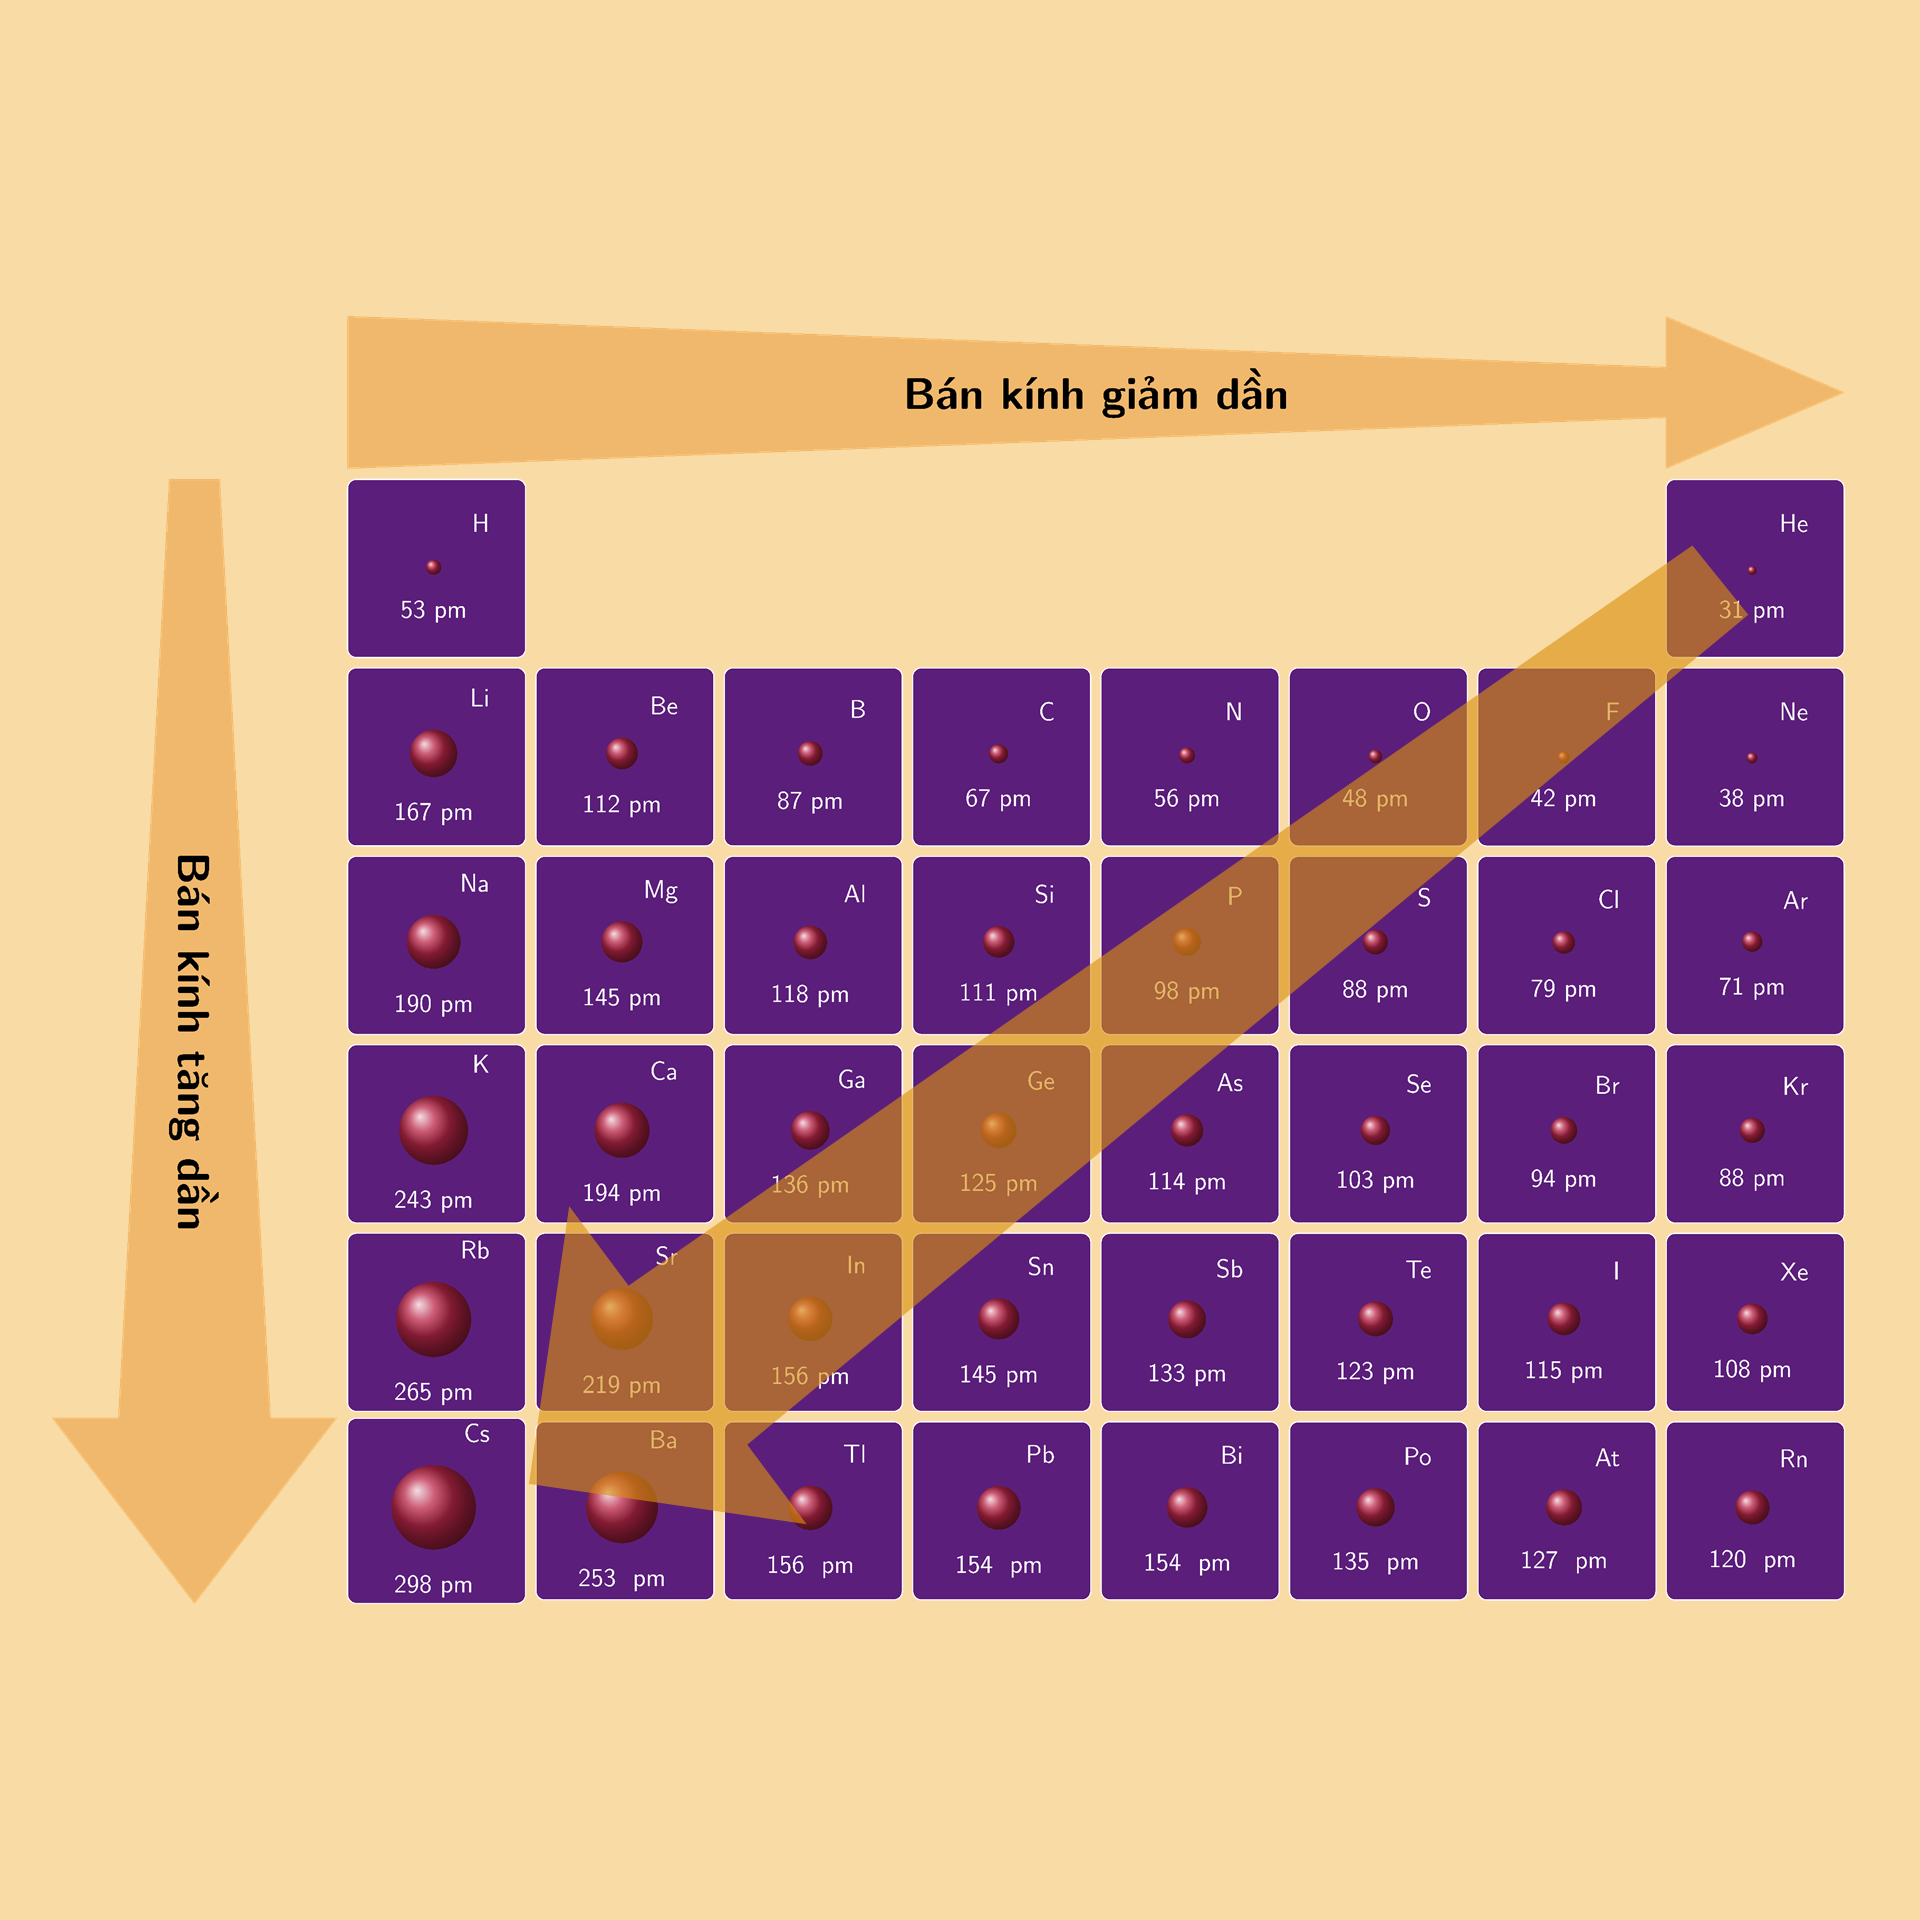
\includegraphics[width 	=8cm]{Images/anhminhoa/xuhuongbk.png}
	\end{center}
	\nhanmanh{Bài toán 2: So sánh bán kính ion}
	\GSND[\bfseries][\faBook][\maunhan]{Quy luât 1:}
%	\taodongke[\maunhan][1.12]{16}
	So với nguyên tử trung hòa
	\begin{enumerate}
		\item Khi một nguyên tử nhường e (cation) thì bán kính sẽ giảm đi
		\item Khi một nguyên tử nhận e (anion) thì bán kính nguyên tử sẽ tăng lên
	\end{enumerate}
	Do vây, đối với cùng nguyên tố thì:
	\begin{center}
		\boxct{Bán kính$_{cation}$ < bán kính $_{\text{nguyên tử}}$ < bán kính $_{anion}$}
	\end{center}
	\GSND[\bfseries][\faBook][\maunhan]{Quy luât 2:}
%	\taodongke[\maunhan][1.12]{18}
	Các ion có cùng số electron
	\begin{enumerate}
		\item Cation có điện tích càng lớn thì bán kính càng nhỏ
		\item Anion có điện tích càng lớn thì bán kính càng lớn
	\end{enumerate}
% \taodongke[\maunhan][1.12]{16}
\end{dangntd}
\newpage
\GSND[\bfseries][\faBookReader][\maudam]{Ví dụ mẫu:}
%%%==============VD_01===================%%%
\begin{vd}
	Hãy sắp xếp các nguyên tố $_{20}Ca$, $_{4}Be$, $_{12}Mg$ theo chiều tăng dần bán kính nguyên tử?
	\loigiai{
	Dựa vào  số hiệu nguyên tử các em viết cấu hình electron của các nguyên tử \Muiten{->} vị trí \Muiten{->} phác thảo lên bảng tuần hoàn  đưa ra quy luật biến đổi tính chất\\
	Ta có:\\
	$_{20}Ca: 1s^{2}2s^{2}2p^{6}3s^{2}3p^{6}4s^{2}$ \Muiten{->} Ca thuộc chu kì 4, nhóm IIA\\
	$_{4}Be: 1s^{2}2s^{2}$ \Muiten{->} Be thuộc chu kì 2, nhóm IIA\\
	$_{12}Mg: 1s^{2}2s^{2}2p^{6}3s^{2}$ \Muiten{->} Mg thuộc chu kì 3, nhóm IIA\\
	Ba nguyên tố Ca, Be, Mg thuộc cùng một nhóm nên chiều bán kính tăng dần là: Be < Mg < Ca
	}
\end{vd}
%%%==============VD_02===================%%%
\begin{vd}
	Hãy sắp xếp các nguyên tố $_{11}Na$, $_{17}Cl$, $_{15}P$, $_{13}Al$ theo chiều tăng dần bán kính nguyên tử?
	\sodongkevd[10]
\end{vd}
%%%==============VD_03===================%%%
\begin{vd}
	Hãy sắp xếp các nguyên tố $_{8}O$, $_{15}P$, $_{13}Al$, $_{20}Ca$, $_{19}K$ theo chiều tăng dần bán kính nguyên tử?
	\sodongkevd[10]
\end{vd}
%%%==============VD_04===================%%%
\begin{vd}
	Cho điện tích hạt nhân $O(Z=8), \mathrm{Na}(Z=11), \mathrm{Mg}(Z=12), \mathrm{Al}(Z=13)$ và các hạt vi mô: $O^{2-}, \mathrm{Al}^{3+}, \mathrm{Al}, \mathrm{Na}, \mathrm{Mg}^{2+}, \mathrm{Mg}$. Dãy nào sau đây được xếp đúng thứ tự bán kính hạt?
	\sodongkevd[15]
\end{vd}
%%%==============VD_05===================%%%
\begin{vd}
	Cho điện tích hạt nhân $O(Z=8), \mathrm{F}(Z=9), \mathrm{Mg}(Z=12), \mathrm{Al}(Z=13),\mathrm{S}(Z=16),\mathrm{Cl}(Z=17),\mathrm{K}(Z=19),\mathrm{Ca}(Z=20)$.Hãy sắp xếp dãy các ion sau: $\mathrm{S}^{2-},\mathrm{Cl}^{-},\mathrm{K}^{+},\mathrm{Ca}^{2+},\mathrm{Al}^{3+},\mathrm{Mg}^{2+},\mathrm{O}^{2-},\mathrm{F}^{-} $ theo chiều tăng dần của bán kính?
	\sodongkevd[15]
\end{vd}
%%%==========Nội dung file thứ 2===============%%%
\chapter{Liên kết hóa học}
\section{Quy tắc Octet}
\begin{mtbh}
	\begin{itemize}
		\item Trình bày được quy tắc octet với các nguyên tố nhóm $A$.
		\item Vận dụng được quy tắc octet trong quá trình hình thành liên kết hoá học ở các nguyên tố nhóm $A$.
	\end{itemize}
\end{mtbh}
\subsection{Kiến thức cần nhớ}
\begin{hoplythuyet}
	\GSND[\bfseries\sffamily][\faStar][\maunhan]{Liên kết hóa học:}
	Liên kết hóa học là sụ kết hợp giữa các nguyên tử tạo thành phân tử hay tinh thể bền vững hơn.
	\GSND[\bfseries\sffamily][\faStar][\maunhan]{Quy tắc octet:}
	Trong quá trình hình thành liên kết hóa học, nguyên tử của các nguyên tố nhóm A có xu hương tạo thành lớp vỏ ngoài cùng có 8 electron tương ứng với khí hiếm gần nhất (hoặc 2 electron với khí hiếm helium).
\end{hoplythuyet}
\begin{notegsnd}
	Không phải mọi trừờng hợp, nguyên tử của các nguyên tố khi tham gia liên kết đều tuân theo quy tắc octet. Người ta nhận thấy một số phân tủ không tuân theo quy tắc octet. Ví dụ: $\mathrm{NO}, \mathrm{BH}_3$, $S F_6, \ldots$
\end{notegsnd}

\columnratio{0.65}
\begin{paracol}{2}
	\begin{hoplythuyet}
		\GSND[\bfseries\sffamily][\faStar][\maunhan]{Liên kết hóa học:}
		Liên kết hóa học là sụ kết hợp giữa các nguyên tử tạo thành phân tử hay tinh thể bền vững hơn.
		\GSND[\bfseries\sffamily][\faStar][\maunhan]{Quy tắc octet:}
		Trong quá trình hình thành liên kết hóa học, nguyên tử của các nguyên tố nhóm A có xu hương tạo thành lớp vỏ ngoài cùng có 8 electron tương ứng với khí hiếm gần nhất (hoặc 2 electron với khí hiếm helium).
	\end{hoplythuyet}
	\switchcolumn 
	\begin{vdnote}
		Hai nguyên tử H liên kết với nhau tạo thành phân tử $H_2$ bền vững hơn nguyên tử H
	\end{vdnote}
	\begin{vdnote}
		Nguyên tử chlorine với cấu hình electron là $[\mathrm{Ne}] 3 \mathrm{~s}^2 3 \mathrm{p}^5$, có 7 electron ở lớp vỏ ngoài cùng.Khi hình thành liên kết hoá học chlorine nhận thêm 1 electron để đạt được lớp vỏ có 8 electron ở lớp ngoài cùng như của khí hiếm $\mathrm{Ar}$ (thay vì $\mathrm{Cl}$ phải nhường đi 7 electron để có lớp vỏ ngoài cùng là $2 \mathrm{~s}^2 2 \mathrm{p}^6$ - khó khăn hơn rất nhiều)
	\end{vdnote}
\end{paracol}

\newcommand{\ngoacvuongtron}[2][]{
	\begin{tikzpicture}[declare function={d=-4pt;},node distance=-d]
		\node (name) {#2};
		\node[anchor = base, above right =of name,shift={(-2pt,-5pt)}](plus) {$#1$};
		\draw[rounded corners=-d-1pt] (name.north west)--([xshift=d]name.north west)|-($(name.south west) +(0,0)$);
		\draw[rounded corners=-d-1pt] (name.north east)--([xshift=-d]name.north east)|-($(name.south east) +(0,0)$);
	\end{tikzpicture}
}
\newpage
\GSND[\bfseries\sffamily][\faStar][\maunhan]{Giải thích sự hình thành liên kết}
\columnratio{0.5}
\begin{paracol}{2}
	%%%================ Giải thích sự hình thành ion Cl ================%%%
	\begin{vdnote}
		Nguyên tử chlorine với cấu hình electron là $[Ne]3s^23p^5$, có 7 electron ở lớp ngoài cùng. Vậy có xu hướng nhận thêm 1 electron để đạt cấu hình bền vững giống khí hiếm Ar (hình \ref{ion_Cl})
	\end{vdnote}
	\begin{center}
		\begin{tikzpicture}[declare function ={k=5cm;},node distance=1.5cm]
			\node at (0:0) (Cl) {
				\begin{tikzpicture}[declare function={r=.5 cm;}]
					\tikzstyle{mystyle} = [draw=red,inner sep = 0pt,anchor=center, baseline]
					\path (0:0) coordinate (O);
					\fill[ball color=red!50](O) circle (r -.25 cm);
					\node[font=\tiny] at (O) {\textbf{+17}};
					\draw[mystyle] (O) circle (r+0.25cm);
					\foreach \g in {0,45,90,135,180,225,270,315}{\fill[ball color =\mauphu!50] (\g:{r+0.25cm}) circle (1pt);}
					\draw[mystyle] (O) circle (r+0.25*2cm);
					\foreach \g in {45,90,135,180,225,270,315}{\fill[ball color =\mauphu!50] (\g:{r+0.25*2cm}) circle (1pt);}
					\draw[mystyle] (O) circle (r);
					\foreach \g in {90,-90}{\fill[ball color =\mauphu!50] (\g:r) circle (1pt);}
				\end{tikzpicture}
			};
			\node[yshift=7pt] at (0:k)(ion-Cl) {
				\ngoacvuongtron[-]{\begin{tikzpicture}[declare function={r=.5 cm;},scale=1.2]
						\tikzstyle{mystyle} = [text centered, draw=red,inner sep = 0pt]
						\path (0:0) coordinate (O);
						\fill[ball color=red!50](O) circle (r -.25 cm);
						\node[font=\tiny] at (O) {\textbf{+17}};
						\draw[mystyle] (O) circle (r+0.25cm);
						\foreach \g in {0,45,90,135,180,225,270,315}{\fill[ball color =\mauphu!50] (\g:{r+0.25cm}) circle (1pt);}
						\draw[mystyle] (O) circle (r+0.25*2cm);
						\foreach \g in {0,45,90,135,180,225,270,315}{\fill[ball color =\mauphu!50] (\g:{r+0.25*2cm}) circle (1pt);}
						\draw[mystyle] (O) circle (r);
						\foreach \g in {90,-90}{\fill[ball color =\mauphu!50] (\g:r) circle (1pt);}
				\end{tikzpicture}}
			};
			\draw[-latex,line width=1pt] (Cl.east)--([yshift=-7pt]ion-Cl.west)node[midway,pos =0.5,above,font=\sf\small,yshift=-2pt]{nhận}node[midway,pos =0.5,below,font=\sf\small,yshift=2pt]{1 electron};
			\node [below of= Cl,font=\bfseries\small] {Cl};
			\node [below of= ion-Cl,font=\bfseries\small,shift={(-6pt,-9pt)}] {\text{Cl$^{-}$}};
		\end{tikzpicture}
		\captionof{figure}{Sơ đồ nguyên tử Cl nhận thêm 1 eclectron vào lớp ngoài cùng \label{ion_Cl}}
	\end{center}
	\switchcolumn
	%%%================Giải thích sự hình thành ion Na================%%%
	\begin{vdnote}
		Nguyên tử Sodium với cấu hình $[Ne]3s^1$, có 1 electron ở lớp ngoài cùng .Vậy xu hướng khi hình thành liên kết là nhường đi 1 electron để đạt được cấu hình electron giống khí hiếm Ne.(hình \ref{ion_Na})
	\end{vdnote}
	\begin{center}
		\begin{tikzpicture}[declare function ={k=5cm;},node distance=1.5cm]
			\node at (0:0) (Na) {
				\begin{tikzpicture}[declare function={r=.5 cm;}]
					\tikzstyle{mystyle} = [draw=red,inner sep = 0pt,anchor=center, baseline]
					\path (0:0) coordinate (O);
					\fill[ball color=red!50](O) circle (r -.25 cm);
					\node[font=\tiny] at (O) {\textbf{+11}};
					\draw[mystyle] (O) circle (r+0.25cm);
					\foreach \g in {0,45,90,135,180,225,270,315}{\fill[ball color =\mauphu!50] (\g:{r+0.25cm}) circle (1pt);}
					\draw[mystyle] (O) circle (r+0.25*2cm);
					\foreach \g in {0}{\fill[ball color =\mauphu!50] (\g:{r+0.25*2cm}) circle (1pt);}
					\draw[mystyle] (O) circle (r);
					\foreach \g in {90,-90}{\fill[ball color =\mauphu!50] (\g:r) circle (1pt);}
				\end{tikzpicture}
			};
			\node[yshift=7pt] at (0:k)(ion-Na) {
				\ngoacvuongtron[+]{\begin{tikzpicture}[declare function={r=.5 cm;},scale=1.2]
						\tikzstyle{mystyle} = [text centered, draw=red,inner sep = 0pt]
						\path (0:0) coordinate (O);
						\fill[ball color=red!50](O) circle (r -.25 cm);
						\node[font=\tiny] at (O) {\textbf{+11}};
						\draw[mystyle] (O) circle (r+0.25cm);
						\foreach \g in {0,45,90,135,180,225,270,315}{\fill[ball color =\mauphu!50] (\g:{r+0.25cm}) circle (1pt);}
						\draw[mystyle] (O) circle (r);
						\foreach \g in {90,-90}{\fill[ball color =\mauphu!50] (\g:r) circle (1pt);}
				\end{tikzpicture}}
			};
			\draw[-latex,line width=1pt] (Na.east)--([yshift=-7pt]ion-Na.west)node[midway,pos =0.5,above,font=\sf\small,yshift=-2pt]{nhường}node[midway,pos =0.5,below,font=\sf\small,yshift=2pt]{1 electron};
			\node [below of= Na,font=\bfseries\small] {Na};
			\node [below of= ion-Na,font=\bfseries\small,shift={(-6pt,-9pt)}] {\text{Na$^{+}$}};
		\end{tikzpicture}
		\captionof{figure}{Sơ đồ nguyên tử Na nhường đi 1 eclectron  \label{ion_Na}}
	\end{center}
\end{paracol}

\columnratio{0.5}
\begin{paracol}{2}
%%%================Giải thích sự hình thành phân tử H2================%%%		
	\begin{vdnote}
		Phân tử $\mathrm {H_2}$ được hình thành từ hai nguyên tử H bởi sự góp chung electron (hình \ref{hthidro})
	\end{vdnote}
	\begin{center}
		\tikzstyle{mystyle} = [draw=\mauphu!90!black,inner sep = 0pt,anchor=center, baseline,fill=\mauphu!90,opacity=.5,line width=.8pt]
		\begin{tikzpicture}[declare function ={k=1.8cm;},node distance=.5pt and .5pt]
			\node at (0:0) (H1) {
				\begin{tikzpicture}[declare function={r=.5 cm;}]
					\path (0:0) coordinate (O);
					\fill[ball color=\mauphu!90](O) circle (r -.25 cm);
					\node[font=\tiny] at (O) {\textbf{+1}};
					\filldraw[mystyle] (O) circle (r+0.25cm);
					\foreach \g in {25}{\fill[ball color =\mauphu!90] (\g:{r+0.25cm}) circle (1.5pt);}
				\end{tikzpicture}
			};
			\node [below=of H1]{\bf H};
			\node at (0:k)(H2) {
					\begin{tikzpicture}[declare function={r=.5 cm;}]
					\path (0:0) coordinate (O);
					\fill[ball color=\mauphu!90](O) circle (r -.25 cm);
					\node[font=\tiny] at (O) {\textbf{+1}};
					\filldraw[mystyle] (O) circle (r+0.25cm);
					\foreach \g in {205}{\fill[ball color =\mauphu!90] (\g:{r+0.25cm}) circle (1.5pt);}
				\end{tikzpicture}
			};
			\node [below=of H2]{\bf H};
			\node at (0:{3*k})(H3){
			\begin{tikzpicture}[declare function={r=.5 cm;}]
				\path (0:0) coordinate (O);
				\fill[ball color=\mauphu!90](O) circle (r -.25 cm);
				\node[font=\tiny] at (O) {\textbf{+1}};
				\filldraw[mystyle] (O) circle (r+0.25cm);
				\foreach \g in {-10}{\fill[ball color =\mauphu!90] (\g:{r+0.12cm}) circle (1.5pt);}
			\end{tikzpicture}
			};
			\node at (0:{3.68*k})(H4){
				\begin{tikzpicture}[declare function={r=.5 cm;}]
					\path (0:0) coordinate (O);
					\fill[ball color=\mauphu!90](O) circle (r -.25 cm);
					\node[font=\tiny] at (O) {\textbf{+1}};
					\filldraw[mystyle] (O) circle (r+0.25cm);
					\foreach \g in {170}{\fill[ball color =\mauphu!90] (\g:{r+0.12cm}) circle (1.5pt);}
				\end{tikzpicture}
			};
			\filldraw[-{Latex[length=5mm]},line width=6pt,draw=\mauphu,] (H2.east)--(H3.west) ;
			\node [below=of H3,xshift={.34*k}]{ $\mathbf {H_2}$};
		\end{tikzpicture}
		\captionof{figure}{Sự góp chung electron trong phân tử hiđro \label{hthidro}}
	\end{center}
		\switchcolumn
	%%%================Giải thích sự hình thành phân tử N2================%%%
	\begin{vdnote}
		Phân tử $\mathrm {N_2}$ được hình thành từ hai nguyên tử N bởi sự góp chung của 3 cặp electron (hình \ref{htnito})
	\end{vdnote}
	\begin{center}
		\tikzstyle{mystyle} = [draw=\mycolor!90!black,inner sep = 0pt,anchor=center, baseline,fill=\mycolor!90,opacity=.3,line width=.8pt]
		\begin{tikzpicture}[declare function ={k=2.5cm;R=1.2cm;},node distance=.5pt and .5pt]
			\node at (0:0) (N1) {
				\begin{tikzpicture}[declare function={r=.5 cm;}]
					\path (0:0) coordinate (O);
					\fill[ball color=\mycolor!90](O) circle (r -.25 cm);
					\node[font=\tiny] at (O) {\textbf{+7}};
					\filldraw[mystyle] (O) circle (r);
					\foreach \g in {90,-90}{\fill[ball color =\mycolor!70] (\g:{r}) circle (1.5pt);}
					\filldraw[mystyle] (O) circle (r+0.25cm);
					\foreach \g in {170,-170,45,-45,0}{\fill[ball color =\mycolor!90] (\g:{r+0.25cm}) circle (1.5pt);}
				\end{tikzpicture}
			};
%	
			\node at (0:.5*k) (plus){\large +};
			\node at (0:k) (N2) {
				\begin{tikzpicture}[declare function={r=.5 cm;}]
					\path (0:0) coordinate (O);
					\fill[ball color=\mycolor!90](O) circle (r -.25 cm);
					\node[font=\tiny] at (O) {\textbf{+7}};
				\begin{scope}[transform canvas={xscale=-1}]
					\filldraw[mystyle] (O) circle (r);
					\foreach \g in {90,-90}{\fill[ball color =\mycolor!70] (\g:{r}) circle (1.5pt);}
					\filldraw[mystyle] (O) circle (r+0.25cm);
					\foreach \g in {170,-170,45,-45,0}{\fill[ball color =\mycolor!90] (\g:{r+0.25cm}) circle (1.5pt);}
				\end{scope}
				\end{tikzpicture}
			};
			
			\node at (0:{2.4*k}) (N3) {
				\begin{tikzpicture}[declare function={r=.5 cm;}]
					\path (0:0) coordinate (O);
					\fill[ball color=\mycolor!90](O) circle (r -.25 cm);
					\node[font=\tiny] at (O) {\textbf{+7}};
					\begin{scope}[transform canvas={xscale=1}]
						\filldraw[mystyle] (O) circle (r);
						\foreach \g in {90,-90}{\fill[ball color =\mycolor!70] (\g:{r}) circle (1.5pt);}
						\filldraw[mystyle] (O) circle (r+0.25cm);
						\foreach \g in {170,-170}{\fill[ball color =\mycolor!90] (\g:{r+0.25cm}) circle (1.5pt);}
					\end{scope}
				\end{tikzpicture}
			};
				\node at (0:{2.90*k}) (N4) {
				\begin{tikzpicture}[declare function={r=.5 cm;}]
					\path (0:0) coordinate (O);
					\fill[ball color=\mycolor!90](O) circle (r -.25 cm);
					\node[font=\tiny] at (O) {\textbf{+7}};
					\begin{scope}[transform canvas={xscale=-1}]
						\filldraw[mystyle] (O) circle (r);
						\foreach \g in {90,-90}{\fill[ball color =\mycolor!70] (\g:{r}) circle (1.5pt);}
						\filldraw[mystyle] (O) circle (r+0.25cm);
						\foreach \g in {170,-170}{\fill[ball color =\mycolor!90] (\g:{r+0.25cm}) circle (1.5pt);}
					\end{scope}
				\end{tikzpicture}
			};
			\node at (0:{2.4*k+.56cm}) {\tikz{\fill[ball color =\mycolor!90]circle (1.45pt);}};
			\node at (0:{2.4*k+.7cm}) {\tikz{\fill[ball color =\mycolor!90]circle (1.45pt);}};
			\node at ([yshift=4pt]0:{2.4*k+.57cm}) {\tikz{\fill[ball color =\mycolor!90]circle (1.45pt);}};
			\node at ([yshift=4pt]0:{2.4*k+.68cm}) {\tikz{\fill[ball color =\mycolor!90]circle (1.45pt);}};
			\node at ([yshift=-4pt]0:{2.4*k+.57cm}) {\tikz{\fill[ball color =\mycolor!90]circle (1.45pt);}};
			\node at ([yshift=-4pt]0:{2.4*k+.68cm}) {\tikz{\fill[ball color =\mycolor!90]circle (1.45pt);}};
			\filldraw[-{Latex[length=5mm]},line width=6pt,draw=\mycolor,] ([xshift=.5cm]N2.east)--([xshift=-.5cm]N3.west) ;
			\node at ([yshift=-4pt]0:{2.4*k+.68cm}) {\tikz{\fill[ball color =\mycolor!90]circle (1.45pt);}};
			\node at ([yshift=-R]0:0) {\large N};
			\node at ([yshift=-R]0:{k}) {\large N};
			\node at ([yshift=-R]0:{2.65*k}) {\large $\mathbf{N_2}$};
		\end{tikzpicture}
		\captionof{figure}{Sự góp chung electron trong phân tử nitơ \label{htnito}}
	\end{center}
\end{paracol}
\subsection{Bài tập}
%%%===============Câu_01=======================%%%		
\begin{ex}[][Quy tắc octet]
	Biết phân tử magnesium được hình thành từ các ion $Mg^{2+}$ và ion $O^{2-}$.Vận dụng quy tắc octet, trình bày sự hình thành các ion trên từ những nguyên tử tương ứng.
	\huongdan{
	\begin{itemize}
		\item Mg (Z=12):$1s^22s^22p^63s^2$ (có 2 electron ở lớp ngoài cùng) $\Rightarrow$ $Mg \longrightarrow$ $Mg^{2+} + 2e$
		\item O (Z=8):$1s^22s^2p^4$ (có 6 electron ở lớp ngoài cùng) $\Rightarrow$ $O + 2e \longrightarrow$ $O^{2-} $
	\end{itemize}
	
	}
\end{ex}
%%%===============Câu_02=======================%%%		
\begin{ex}[][Quy tắc octet]
	Cho các nguyên tử của các nguyên tố sau:Na(Z=11), Cl(Z=17), Ne(Z=10), Ar(Z=18).Những nguyên tử nào trong các nguyên tử trên có lớp electron bền vững.
	\huongdan{
		\begin{multicols}{2}
			\begin{itemize}
			\item Na (Z=11):$1s^22s^22p^63s^1$ 
			\item Cl (Z=17):$ 1s^22s^22p^63s^23p^5$
			\item Ne (Z=10):$ 1s^22s^22p^6$
			\item Ar (Z=18):$ 1s^22s^22p^63s^23p^6$
		\end{itemize}
		\end{multicols}
	}
\end{ex}















%\newpage
%\setchemfig{%
%	atom sep= 2em,
%	bond offset=2pt,
%	compound sep=5em
%}

%\schemestart
%\chemname{\chemfig{
%H-@{N}\charge{0:2pt=\:}{N}(-[6]H)-[2]H
%}}{\scriptsize\quad\quad Ammonia\vphantom{aa}}
%\+
%\chemfig{
%@{H}\charge{45:3pt=$\scriptstyle+$}{H}
%}
%\arrow(.mid east--.mid west)[,.7,-latex]
%\chemname{\ngoacvuongtron{\chemfig{
%			H-N(-[2]H)(-[6]H)-[,,,,-stealth]H
%}}}{\scriptsize Ammonium\quad}
%\schemestop
%
%\chemmove[shorten <=4pt,shorten >=4pt,-latex] {
%\draw ([shift={(-25:3.5pt)}]N.25).. controls +(80:8mm) and +(100:8mm)..([shift={(29:3.5pt)}]H.65)
%;}
%%%%=============Tinh thể NaCl===================%%%
%\begin{tikzpicture}[node distance=0pt]
%	% Định dạng cho cột của bảng
%	\tikzset{%
%		%% Định dạng ô
%		mynode/.style={%
%			circle,
%			ultra thin,
%			minimum height=0.65cm,
%			minimum width=0.65cm,
%			align=center
%		},
%		mymatrix/.style={%
%			matrix of nodes,
%			ampersand replacement=\&,
%			inner sep =5pt,
%			nodes in empty cells,
%			fill =\mycolor!15,
%			row sep=-3-\pgflinewidth,
%			column sep=-3-\pgflinewidth,
%			nodes={mynode}
%		}
%	}
%	\matrix(Bang)[mymatrix]{%
%	\&\&\&\&\&\\
%	\&\&\&\&\&\\
%	\&\&\&\&\&\\
%	\&\&\&\&\&\\
%	\&\&\&\&\&\\
%	};
%\foreach \x in {1,3,5}{
%	\foreach \y in {1,3,5}{
%	\fill [ball color=\maunhan!70 ] (Bang-\x-\y) circle (0.3cm) node[font=\tiny\sffamily\bfseries\color{white}](Na) {Na} ;
%	\node [font=\fontsize{5pt}{3pt}\selectfont\sffamily\bfseries\color{white}] at ([shift={(60:4.8pt)}]Bang-\x-\y) {+};
%	}
%}
%\foreach \x in {2,4}{
%	\foreach \y in {2,4,6}{
%		\fill [ball color=\maunhan!70 ] (Bang-\x-\y) circle (0.3cm);
%	}
%}
%\foreach \x in {1,3,5}{
%	\foreach \y in {2,4,6}{
%		\fill [ball color=\maudam!70 ] (Bang-\x-\y) circle (0.2cm);
%	}
%}
%\foreach \x in {2,4}{
%	\foreach \y in {1,3,5}{
%		\fill [ball color=\maudam!70 ] (Bang-\x-\y) circle (0.2cm);
%	}
%}
%\end{tikzpicture}
%%%==========Nội dung file thứ 3===============%%%
\newenvironment{cacbuoc}{\begin{enumerate}[label= \color{\maunhan}\bfseries\fontfamily{qag}\selectfont{\faAdjust\;Bước \arabic*:},itemsep=0pt,wide=0cm,leftmargin=0.5cm,topsep=0pt]
	}{\end{enumerate}}
\newtcolorbox{body}{%
	enhanced,
	before skip=1cm,
	breakable,
	colback=\mycolor!20,
	enhanced jigsaw,opacityback=0,opacitybacktitle=0,
	opacityback=0,
	colframe=\mycolor
}
\renewcommand{\thesubsubsection}{\Roman{subsubsection}}
\titlespacing*{\subsection}{3pt}{0pt}{-5pt}
\titlespacing*{\subsubsection}{3pt}{5pt}{-5pt}
\titlespacing*{\paragraph}{0cm}{0cm}{-5pt}
\setcounter{chapter}{3}
\chapter{Phản ứng Oxi hóa - khử}
\section{Số Oxi hóa - Cân bằng phản ứng oxi hóa khử}
\subsection{Kiến thức cần nhớ}
\begin{body}
	\subsubsection{Số oxi hóa}
	\begin{dn}
		\indam{Số oxi hóa} của một nguyên tử một nguyên tố trong hơp chất là \indam{điện tích} của nguyên tử nguyên tố đó với giả định đây là hợp chất ion.
	\end{dn}
	\subsubsection{Cách xác định số oxi - hóa}
	\begin{enumerate}
		\item \indam{Quy tắc 1:}
		Trong đơn chất, số oxi hóa của các nguyên tố bằng 0.\\
		VD: $\overset{0}{\mathrm{H}_{2}}$, $\overset{0}{\mathrm{Na}}$, $\overset{0}{\mathrm{O}_{3}}$, $\ldots$
		\item \indam{Quy tắc 2:}
		Trong một phân tử,tổng số oxi hóa  của các nguyên tố nhân với số nguyên tử của từng nguyên tố bằng 0\\
		\item \indam{Quy tắc 3:} 
		\begin{itemize}
			\item Trong các ion \indam{đơn nguyên tử}, số oxi hóa của các nguyên tố bằng điệnu tích của ion đó\\
			\item Trong ion \indam{đa nguyên tử}, tổng số oxi hóa các nguyên tố nhân với số nguyên tử của từng nguyên tố bằng điện tích của ion
		\end{itemize}
		\item \indam{Quy tắc 4:} \\
		\begin{itemize}
			\item Trong đa số các hợp chất, số oxi hóa của hydrogen bằng +1 , trừ hydride kim loại ($NaH$, $CaH_2$)\\
			\item Số oxi hóa của oxygen bằng $-\mathrm{2}$, trừ trường hợp $\overset{+1}{\mathrm{O}_{}}\overset{\vphantom{-1}}{\mathrm{F}_{2}}$ và peoxit $\left(\overset{\vphantom{+1}}{\mathrm{Na}_{2}}\overset{-1}{\mathrm{O}_{2}}\right)$, superoxide $\left(\overset{\vphantom{+1}}{\mathrm{K}_{}}\overset{-\tfrac{1}{2}}{\mathrm{O}_{2}}, \ldots\right)$.\\
			\item Các nguyên tố nhóm IA, IIA luôn có số oxi hóa $+1,+2$, số oxi hóa của $\mathrm{Al}$ là +3 . Số oxi hóa của nguyên tử nguyên tố fluorine trong các hợp chất bằng -1
		\end{itemize}
	\end{enumerate}
	\subsubsection{Phản ứng Oxi hóa - khử}
	\paragraph{Sự oxi hóa-sự khử}
	\begin{mylt}
		\begin{enumerate}[label = \indam{\alph*)}]
			\item \indam{Sự oxi hóa} là sự nhường electron, là sự tăng số oxi hóa.\\
			\indam{Ví dụ:} $\overset{0}{Mg} \rightarrow Mg^{2+} + 2e$
			\item \indam{Sự khử} là sự thu electron, là sự giảm electron.\\
			\indam{Ví dụ:} $Cu^{2+} +2e \rightarrow Cu $
		\end{enumerate}
	\end{mylt}
	\paragraph{Chất oxi hóa - chất khử}
	\begin{mylt}
		\begin{enumerate}[label = \indam{\alph*)}]
			\item \indam{Chất oxi hóa} là chất thu electron.là chất chứa nguyên tố có số oxi hóa giảm sau phản ứng.\\
			\indam{Chất oxihóa} còn gọi là chất \indam{bị khử}.
			\item \indam{Chất khử} là chất nhường electron, là chất có số oxi hóa tăng sau phản ứng\\
			\indam{Chất khử} còn gọi là chất \indam{bị oxi hóa}.
		\end{enumerate}
	\end{mylt}
	\begin{vdnote}
		$ \overset{0}{Mg} + \overset{+2}{Cu}SO_{4} \rightarrow\overset{+2}{Mg}SO_{4}  + \overset{0}{Cu}$.\\
		$Cu^{2+}$ nhận electron, là chất oxi hóa ( số oxi hóa giảm từ +2 về 0).
		$Mg$ nhường electron, là chất khử (số oxi hóa tăng từ 0 lên +2)
	\end{vdnote}
	\begin{vdnote}
		$\overset{+3}{Fe_2}\overset{\vphantom{+3}}{O_3} + 3\overset{+2}{C}O$ $\longrightarrow$ $ 2 \overset{0}{Fe} + 3\overset{+4}{C}O_2$
	\end{vdnote}
	\paragraph{Phản ứng Oxi hóa - khử }
	\begin{mylt}
		\indam{Phản ứng oxi - hóa khử } là phản ứng hóa học trong đó có sự chuyển electron giữa các chất phản ứng.\\
		Nếu dựa vào sự thay đổi số oxi hóa thì phản ứng oxi hóa-khử là phản ứng hóa học trong đó có sự  thay đổi số oxi hóa của một số nguyên tố.\\
		
		\begin{vdnote}
			\[\begin{tikzpicture}
				\tikzstyle{mynode} =[
				font=\normalsize,
				line width =.8pt,
				anchor=center,
				align =center,
				]
				%%%==================%%%
				\tikzstyle{mymatrix} = [
				matrix of nodes,
				nodes in empty cells,
				nodes={mynode},
				column sep=-\pgflinewidth,
				row sep = -\pgflinewidth,
				minimum width = .5cm,
				minimum height = .6cm,
				column 4/.style={
					minimum width = .7cm,
				},
				]
				%%%=======================================================%%%
				\matrix(m) [mymatrix]{
					Mg & + & $CuSO_4$ & [-.7cm]\muiten[][][0.7]{->}& $MgSO_4$ & + & Cu\\
				};
				\node(0)[yshift=4pt,\maunhan] at (m-1-1.north){0};
				\node(2)[xshift =-8pt,yshift=4pt,\maunhan] at (m-1-3.north){+2};
				\node[xshift =-8pt,yshift=4pt,\maunhan] at (m-1-5.north){+2};
				\node[yshift=4pt,\maunhan] at (m-1-7.north){0};
				\draw[->,>=stealth,violet,ultra thick](0.90)--++(90:.5cm)-|(2.90) ;
				\path ($(0.90)+(90:.5cm)$)-- ($(2.90)+(90:.5cm)$) node [pos=.5,above,violet]{- 2 e};
			\end{tikzpicture}\]
			Trong phản ứng trên $Mg$ nhường đi 2 electron cho ion $Cu^{+2}$ trở thành ion $Mg^{+2}$ và ion $Cu^{+2}$ nhận  2 electron từ nguyên tử $Mg$ trở thành nguyên tử Cu.
		\end{vdnote}
		%%%===============Môi Trường Matrix=================%%%
	\end{mylt}
	\subsubsection{Cân bằng phản ứng oxi hóa-khử}
	\begin{mylt}
		\GSND[\bfseries\sffamily][\faStar]{Phương pháp thăng bằng electron:}\\
		Phương pháp này dựa trên nguyên tắc:
		\boxct[\mauphu][3pt][\bfseries\sffamily\color{violet}]{Tổng số electron chất khử nhường  = tổng số electron mà chất oxi hóa nhận}
		\indam{\faBook\ Các bước cân bằng:}\vspace{.5cm}
		\begin{vdnote}
			Lập phương trình phản ứng Oxi hóa - khử sau: 
			\[\puhh[$t^{\circ}$]{$Cu$\+ $HNO_3$}{->}{$Cu({NO_3})_2$ \+ $NO\uparrow$ \+ $H_2O$}\]
		\end{vdnote}
		\indam{\itshape Hướng dẫn giải:}
		\begin{cacbuoc}
			\item Xác định số oxi hóa của nguyên tử cóa sự thay đổi số oxi hóa, xác định chất khử, chất oxi hóa
			\[\begin{tikzpicture}
				\tikzstyle{mynode} =[
				font=\normalsize,
				line width =.8pt,
				anchor=center,
				align =center,
				]
				%%%==================%%%
				\tikzstyle{mymatrix} = [
				matrix of nodes,
				nodes in empty cells,
				nodes={mynode},
				column sep=-\pgflinewidth,
				row sep = -\pgflinewidth,
				minimum width = .5cm,
				minimum height = .6cm,
				column 4/.style={
					minimum width = .7cm,
				},
				]
				%%%=======================================================%%%
				\matrix(m) [mymatrix]{
					$Cu$ & + & $HNO_3$ & [-.7cm]\muiten[][][0.7]{->}& $Cu({NO_3})_{2}$ & + & $NO\uparrow$ & + & $H_2O$ \\
				};
				\node(0)[yshift=4pt,\maunhan] at (m-1-1.north){0};
				\node(chatkhu)[yshift=-4pt,\maunhan,font=\footnotesize] at (m-1-1.south){(Chất khử)};
				\node(2)[xshift =-2pt,yshift=4pt,\maunhan] at (m-1-3.north){+5};
				\node(chatoxh)[yshift=-4pt,\maunhan,font=\footnotesize] at (m-1-3.south){(Chất oxi hóa)};
				\node[xshift =-18pt,yshift=4pt,\maunhan] at (m-1-5.north){+3};
				\node[xshift =-8pt,yshift=4pt,\maunhan] at (m-1-7.north){+2};
			\end{tikzpicture}\]
			\item Viết quá trình oxi hóa và quá trình khử
			\[\begin{tikzpicture}
				\tikzstyle{mynode} =[
				font=\normalsize,
				line width =.8pt,
				anchor=center,
				align =center,
				minimum width = 0.4cm,
				minimum height = 1.0cm,
				]
				%%%==================%%%
				\tikzstyle{mymatrix} = [
				matrix of nodes,
				nodes in empty cells,
				nodes={mynode},
				column sep=-\pgflinewidth,
				row sep = 2pt-\pgflinewidth,
				column 1/.style={
					minimum width = 4cm,
					anchor =east,
					align =center,
				},
				]
				%%%=======================================================%%%
				\matrix(m) [mymatrix]{
					\text{Quá trình oxi hóa :} & Cu & [-.5cm]\muiten[][][0.4]{->}& Cu & + & 2e\\
					\text{Quá trình khử :} & N & + & [-.5cm]3e & [-.5cm]\muiten[][][0.4]{->} & NO\\
				};
				\node(0)[yshift=-2pt,\maunhan] at (m-1-2.north){0};
				\node(3)[yshift=-2pt,\maunhan] at (m-1-4.north){+2};
				\node(5)[yshift=-2pt,\maunhan] at (m-2-2.north){+5};
				\node(2)[xshift=-2pt,yshift=-2pt,\maunhan] at (m-2-6.north){+2};
			\end{tikzpicture}\]
			\item Nhân hệ số thích hợp  vào các quá trình  sao cho tổng  số electron chất khử nhường  bằng tổng số electron chất oxi hóa nhận.
			\[\begin{tikzpicture}
				\tikzstyle{mynode} =[
				font=\normalsize,
				line width =.8pt,
				anchor=center,
				align =center,
				minimum width = 0.4cm,
				minimum height = 1.0cm,
				]
				%%%==================%%%
				\tikzstyle{mymatrix} = [
				matrix of nodes,
				nodes in empty cells,
				nodes={mynode},
				column sep=3pt-\pgflinewidth,
				row sep = 2pt-\pgflinewidth,
				column 1/.style={
					minimum width = 4cm,
					anchor =east,
					align =center,
				},
				]
				%%%=======================================================%%%
				\matrix(m) [mymatrix]{
					3 x & Cu & [-.5cm]\muiten[][][0.4]{->}& Cu & + & 2e\\
					2 x & N & + & [-.5cm]3e & [-.5cm]\muiten[][][0.4]{->} & NO\\
				};
				\node(0)[yshift=-2pt,\maunhan] at (m-1-2.north){0};
				\node(3)[yshift=-2pt,\maunhan] at (m-1-4.north){+2};
				\node(5)[yshift=-2pt,\maunhan] at (m-2-2.north){+5};
				\node(2)[xshift=-2pt,yshift=-2pt,\maunhan] at (m-2-6.north){+2};
				\draw[\maunhan,line width=1pt] (m-1-1.north east)--(m-2-1.south east);
			\end{tikzpicture}\]
			\item Đặt các hệ số vào sơ đồ phản ứng. Can bằng số lượng  nguyên tử của các nguyên tố còn lại.
			\[\puhh[$t^{\circ}$]{$3Cu$ \+ ${8HNO_3}_{\text{loãng}}$}{->}{$3Cu({NO_3})_{2}$ \+ $2NO$ \+ $4H_2O$}\]
		\end{cacbuoc}
	\end{mylt}
\end{body}
\newpage
\subsection{Các dạng bài tập}
\begin{dangNTD}{Câu hỏi lý thuyết về phản ứng oxi hóa khử}
\end{dangNTD}
\begin{vdm}
\end{vdm}

\hienthiloigiaivd
%%%=========vd_1=========%%%
\begin{vd}[1][Nhận biết các quá trình vai trò của các chất]Một nguyên tử nhôm (Al) chuyển thành ion $Al^{3+}$ thực hiện :
	\choice
	{%
		nhận thêm 3 electron (quá trình oxi hóa)
	}{%
		nhường đi 3 electron (quá trình khử)
	}{%
		nhận thêm 3 electron (quá trình khử)
	}{%
		\True nhường đi 3 electron (quá trình oxi hóa)
	}
	\loigiai{Quá trình oxi hóa  một chất là làm cho nguyên tử trong chất đó nhường electron hay làm tăng số oxi hóa của nguyên tử trong chất đó.\\
		Quá trình khử  một chất là làm cho nguyên tử trong chất đó nhận electron hay làm giảm số oxi hóa của nguyên tử trong chất đó.\\
		Ta thấy số oxi hóa của nhôm tăng (quá trình oxi hóa) \\
		$\begin{matrix}
			\overset{0}{Al}& \muiten[][][.4]{->} &\overset{+3}{Al} & + & 3e
		\end{matrix}$
	}
\end{vd}
%%%=========vd_2=========%%%
\begin{vd}[2][Nhận biết các quá trình vai trò của các chất]Trong phản ứng : \puhh{$Cl_2$\+ $2KBr$}{->}{$Br_2$\+ 2KCl}, $Cl_2$ đóng vai trò 
	\choice{%
		\True là chất oxi hóa
	}{%
		là chất khử
	}{%
		không bị oxi hóa, không bị khử
	}{%
		vừa bị oxi hóa, vừa bị khử.
	}
	\loigiai{Chất oxi hóa là chất nhận electron hay là chất có số oxi hóa giảm sau phản ứng.\\
		Chất khử là chất nhường electron hay là chất có số oxi hóa tăng sau phản ứng.\\
		Ta thấy số oxi hóa của Cl giảm :\\
		$\begin{matrix}
			Cl_2 & + & 2e & \muiten[][][.4]{->} & 2Cl^{-}
		\end{matrix}$
	}
\end{vd}

%%%=========vd_3=========%%%
\begin{vd}[2][Nhận biết phản ứng oxi hóa khử]
	Phản ứng nào sau đây \indam[black]{không phải} phản ứng oxi hóa khử
	\choice{
		\puhh{$2NaOH$\+ $Cl_2$}{->}{$NaCl$\+$NaClO$\+ $H_2O$}
	}{
		\True \puhh[$t^{\circ}$]{$CaCO_3$}{->}{$CaO$\+$CO_2$}
	}{
		\puhh[$t^{\circ}$]{$2KClO_3$}{->}{$2KCl$\+$3O_2$}
	}{
		\puhh{$Fe$\+ $2HCl$}{->}{$FeCl_2$\+$H_2$}
	}
	\loigiai{%
		Phản ứng oxi hóa - khử là phản ứng  hóa học trong đó có sự thay đổi số oxi hóa.\\
		Phản ứng không phải là phản ứng oxi hóa - khử là phản ứng không có sự thay đổi số oxi hóa của các nguyên tố\\
		Ta có:\\
		$\begin{matrix}
			2NaOH  & + & \overset{0}{Cl}_{2} & \muiten{->} & \overset{\vphantom{+1}}{Na}\overset{-1}{Cl} & + & \overset{\vphantom{+1}}{Na}\overset{+1}{Cl}O  & + & H_2O\\
		\end{matrix}$\\
		$\begin{matrix}
			\overset{\vphantom{+4}}{Ca}\overset{+4}{C}\overset{\vphantom{-2}}{O_3} & \muiten{->}& \overset{+2}{Ca}O & + & \overset{+4}{C}\overset{\vphantom{+4}}{O_2}\\
		\end{matrix}$\\
		$\begin{matrix}
			\overset{\vphantom{-2}}{2K}\overset{+5}{Cl}\overset{\vphantom{-2}}{O_3} & \muiten{->}& \overset{\vphantom{-2}}{2K}\overset{-1}{Cl} & + & 3\overset{-2}{O_2}\\
		\end{matrix}$\\
		$\begin{matrix}
			\overset{0}{Fe}& + & 2\overset{+1}{H}Cl & \muiten{->}& \overset{+2}{Fe}\overset{\vphantom{-2}}{Cl_2} & + & \overset{0}{H_2} \\
		\end{matrix}$\\
		\indam{Nhận xét: }Phản ứng B không có sự thay đổi số oxi hóa của các nguyên tố. $\longrightarrow$ Phản ứng B không phải là phản ứng oxi hóa - khử
	}
\end{vd}


%%%=========vd_4=========%%%
\begin{vd}[2][Nhận biết phản ứng oxi hóa khử]Cho các phản ứng sau đây:
	\begin{enumerate}[a)]
		\item $C + O_{2} \xrightarrow{t^{\circ}} CO_{2}$
		\item $CaO +  H_{2}O \longrightarrow Ca(OH)_{2}$
		\item $CuO + H_{2} \xrightarrow{t^{\circ}} Cu + O_2$
		\item $2KMnO_4 \xrightarrow{t^{\circ}} K_2MnO_4 + MnO_2 + H_2O$
		\item $Cl_2 + 2KOH \longrightarrow KCl + KClO + H_2O$
		\item $Fe_3O_4 + 8HCl \longrightarrow 2FeCl_3 + FeCl_2 + 4H_2O$
	\end{enumerate}
	Số phản ứng thuộc loại phản ứng oxi hóa - khử là:
	\choice{2}{\True 4}{3}{5}
	\loigiai{%
		Phản ứng oxi hóa khử là phản ứng hóa học trong đó có sự thay đổi số oxi hóa của một số nguyên tố.
		\begin{enumerate}[a)]
			\item $\overset{0}{C} + \overset{0}{O}_{2} \xrightarrow{t^{\circ}} \overset{+4}{C}\overset{-2}{O}_{2}$
			\item $\overset{+2}{Ca}\overset{-2}{O} +  \overset{+1}{H_{2}}\overset{-2}{O} \longrightarrow \overset{+2}{Ca}(\overset{-2}{O}\overset{+1}{H})_{2}$
			\item $\overset{+2}{Cu}\overset{-2}{O} + \overset{-2}{H}_{2} \xrightarrow{t^{\circ}} \overset{0}{Cu} + \overset{+1}{H}_2\overset{-2}{O}$
			\item $2K\overset{+7}{Mn}\overset{-2}{O}_4 \xrightarrow{t^{\circ}} K_2\overset{+6}{Mn}O_4 + \overset{0}{O}_2 + \overset{+6}{Mn}O_{2}$
			\item $\overset{0}{Cl}_2 + 2KOH \longrightarrow K\overset{-1}{Cl} + K\overset{+1}{Cl}O + H_2O$
			\item $\overset{+8/3}{Fe_3}\overset{-2}{O_4} + 8\overset{+1}{H}\overset{-1}{Cl} \longrightarrow 2\overset{+3}{Fe}Cl_3 + \overset{+2}{Fe}\overset{-1}{Cl}_2 + 4\overset{+1}{H}_2O$
		\end{enumerate}
		\indam{Nhận xét:} Phản ứng a), c), d), e) có sự thay đổi số oxi hóa của các nguyên tố. $\Rightarrow$ Phản ứng a), c), d), e) là phản ứng oxi hóa - khử 
	}
\end{vd}
%%%=========vd_5=========%%%
\begin{vd}[2][Cân bằng phản ứng oxi hóa khử]Lập phương trình phản ứng oxi hóa - khử sau đây:
	\puhh{ $MnO_2$ \+ $HCl$}{->}{$MnCl_2$ \+ $ Cl_2$ \+ $H_2O$}
	\loigiai{\begin{cacbuoc}
			\item Xác định số oxi hóa của các nguyên tố :\\
			$\overset{+4}{Mn}O_2 + H\overset{-1}{Cl} \longrightarrow \overset{+2}{Mn}Cl_2 + \overset{0}{Cl_2} + H_2O$ 
			\item Quá trình cho - nhận electron\\
			$\begin{matrix}
				2\overset{-1}{Cl} & \longrightarrow& Cl_2 & + & 2e\\
				\overset{+4}{Mn} &  + & 2e & \longrightarrow & \overset{+2}{Mn}
			\end{matrix}$
			\item Đặt hệ số \\
			$\begin{matrix}
				1x|~2\overset{-1}{Cl} & \longrightarrow& Cl_2 & + & 2e\\
				1x|~\overset{+4}{Mn} &  + & 2e & \longrightarrow & \overset{+2}{Mn}
			\end{matrix}$
			\item Phương trình hóa học
			\boxct{$MnO_2 + 4HCl \longrightarrow MnCl_2 + Cl_2 + 2H_2O$}
	\end{cacbuoc}}
\end{vd}
%%%=========vd_6=========%%%
%%%==========================%%%
%%%==========================%%%
\begin{vd}[3][Cân bằng phản ứng oxi hóa - khử][Nguồn:CĐA 2010] Cho phản ứng:
	$\mathrm{Na}_2 SO_3+\mathrm{KMnO}_4+\mathrm{NaHSO}_4 \to \mathrm{Na}_2 SO_4+\mathrm{MnSO}_4+K_2 SO_4+H_2 O$.Tổng hệ số của các chất (là những số nguyên, tối giản) trong phương trình phản ứng là
	\choice
	{23}
	{27}
	{47}
	{31}
	\loigiai{
		\begin{cacbuoc}
			\item Xác định số oxi hóa của các nguyên tố :\\
			$Na_2\overset{+4}{S}O_3$ + $K\overset{+7}{Mn}O_4$ + $NaHSO_4$ $\to$ $Na_2\overset{+6}{S}O_4$ + $\overset{+2}{Mn}SO_4$ + $K_2SO_4$ + $H_2 O$
			\item Quá trình cho - nhận electron\\
			$\begin{matrix}
				\overset{+7}{Mn} &  + & 5e & \longrightarrow & \overset{+2}{Mn}\\
				\overset{+4}{S} & \longrightarrow& \overset{+6}{Mn} & + & 2e
			\end{matrix}$
			\item Đặt hệ số \\
			$\begin{array}{lllll}
				2x|~\overset{+7}{Mn} &  + & 5e & \longrightarrow & \overset{+2}{Mn}\\
				5x|~\overset{+4}{S} & \longrightarrow& \overset{+6}{Mn} & + & 2e
			\end{array}$\\
			\item Phương trình hóa học\\
			Hệ số 5 điền cho S ($5Na_2SO_3$ và $?Na_2SO_4$). Hệ số 2 điền cho Mn ($2KMnO4$ và $2MnO4$).
			
			\GSND[][\faComment]{Phân tích:}Hệ số của $\mathrm{Na}_2 \mathrm{SO}_3, \mathrm{KMnO}_4, \mathrm{MnSO}_4$ và $\mathrm{K}_2 \mathrm{SO}_4$ đã được xác định.\\
			Do gốc $\mathrm{SO}_4^{2-}$ là sản phẩm oxi hóa của $\mathrm{SO}_3^{2-}$ đồng thời cũng là sản phẩm của chất làm nhiệm vụ môi trường $\mathrm{NaHSO}_4$. Do vậy cần tìm hệ số của $\mathrm{Na}_2 \mathrm{SO}_4, \mathrm{NaHSO}_4$ và $\mathrm{H}_2 \mathrm{O}$ bằng phương pháp bảo toàn nguyên tố.
			
			\noindent Đặt $x$ là hệ số của $\mathrm{Na}_2 \mathrm{SO}_4$ và $ y$ là hệ số của $\mathrm{H_2O}$ .\\
			- Bảo toàn số nguyên tử  $H\Rightarrow$ hệ số của $NaHSO_4$ là $2y$\\
			$5\mathrm{Na}_2 SO_3+2\mathrm{KMnO}_4+2y\mathrm{NaHSO}_4 \to x\mathrm{Na}_2 SO_4+2\mathrm{MnSO}_4+K_2 SO_4+yH_2 O$\\
			- Bảo toàn số nguyên tử $S \Rightarrow(5+2 y)=(x+2+1) \Rightarrow(x-2 y)=2$ (*)\\
			- Bảo toàn số nguyên tử $O$
			$\Rightarrow(15+8+8 y)=(4 x+12+y) \Rightarrow(4 x-7 y)=11$(**)\\
			Từ (*) và (**) $\Rightarrow x=8 ; y=3$
			\boxct[\mauphu]{$5\mathrm{Na}_2 SO_3+2\mathrm{KMnO}_4+6\mathrm{NaHSO}_4 \to 8\mathrm{Na}_2 SO_4+2\mathrm{MnSO}_4+K_2 SO_4+3H_2 O$}
		\end{cacbuoc}
	}
\end{vd}
%%%=========Vd7=============%%%
\begin{vd}[2][Cân bằng phản ứng oxi hóa - khử]
	Cân bằng các phản ứng oxi hóa khử sau bằng phương pháp \indam[black]{thăng bằng electron}:
	\begin{enumerate}
		\item $\mathrm{KMnO}_4+\mathrm{HCl} \to \mathrm{MnCl}_2+\mathrm{Cl}_2+\mathrm{KCl}+H_2O$
		\item $K_2\mathrm{Cr}_2O_7+\mathrm{HCl} \to \mathrm{CrCl}_3+\mathrm{Cl}_2+\mathrm{KCl}+H_2O$
	\end{enumerate}
	\loigiai{\begin{enumerate}[(1)]
			\item $\mathrm{KMnO}_4+\mathrm{HCl} \to \mathrm{MnCl}_2+\mathrm{Cl}_2+\mathrm{KCl}+H_2O$
			\begin{cacbuoc}
				\item Xác định số oxi hóa của các nguyên tố :\\
				$K\overset{+7}{Mn}O_4 + H\overset{-1}{Cl} \longrightarrow \overset{+2}{Mn}Cl_2 + \overset{0}{Cl_2} + H_2O$ 
				\item Quá trình cho - nhận electron\\
				$\begin{matrix}
					2\overset{-1}{Cl} & \longrightarrow& Cl_2 & + & 2e\\
					\overset{+7}{Mn} &  + & 5e & \longrightarrow & \overset{+2}{Mn}
				\end{matrix}$
				\item Đặt hệ số \\
				$\begin{array}{lccccc}
					5x\biggl|&2\overset{-1}{Cl} & \longrightarrow& Cl_2 & + & 2e\\
					2x\biggl|&\overset{+7}{Mn} &  + & 5e & \longrightarrow & \overset{+2}{Mn}
				\end{array}$
				\item Phương trình hóa học\\
				Đặt hệ số 2 cho Mn ($2MnCl_2$ và $2KMnO_4$).Đặt hệ số 5 cho Cl ($5Cl_2$ và $?HCl$)\\
				- Bảo toàn K: $\Rightarrow 2KCl $\\
				$\Rightarrow 2\mathrm{KMnO}_4+?\mathrm{HCl} \to 2\mathrm{MnCl}_2+ 5\mathrm{Cl}_2+2\mathrm{KCl}+H_2O$
				\GSND[][\faComment]{Phân tích:}HCl tham gia vào quá trình oxi hóa (tạo ra $5Cl_2$)  và làm môi trường tạo muối ($2MnCl_2$ và $2KCl$ ).Như vậy bảo toàn Cl $\Rightarrow 16HCl $ và bảo toàn H $\Rightarrow 8H_2O $
				\boxct{$2\mathrm{KMnO}_4+16\mathrm{HCl} \to 2\mathrm{MnCl}_2+5\mathrm{Cl}_2+2\mathrm{KCl}+8H_2O$}
			\end{cacbuoc}
			\item $K_2\mathrm{Cr}_2O_7+\mathrm{HCl} \to \mathrm{CrCl}_3+\mathrm{Cl}_2+\mathrm{KCl}+H_2O$
			\begin{cacbuoc}
				\item Xác định số oxi hóa của các nguyên tố :\\
				$K_2\mathrm{\overset{+6}{Cr}}_2O_7+\mathrm{H\overset{-1}{Cl}} \to \mathrm{\overset{+3}{Cr}Cl}_3+\overset{0}{Cl}_2+\mathrm{KCl}+H_2O$ 
				\item Quá trình cho - nhận electron\\
				$\begin{matrix}
					2\overset{+6}{Cr} &  + & 6e & \longrightarrow & 2\overset{+3}{Cr}\\
					2\overset{-1}{Cl} & \longrightarrow& Cl_2 & + & 2e\\
				\end{matrix}$
				\item Đặt hệ số \\
				$\begin{array}{lccccc}
					1x\biggl|&2\overset{+6}{Cr} &  + & 6e & \longrightarrow & 2\overset{+3}{Cr}\\
					3x\biggl|&2\overset{-1}{Cl} & \longrightarrow& Cl_2 & + & 2e\\
				\end{array}$
				\item Phương trình hóa học\\
				Đặt hệ số  cho Cr ( $K_2Cr_2O_7$ và $2CrCl_3$).Đặt hệ số 3 cho Cl ( $3Cl_2$ và $?HCl$).\\
				- Bảo toàn K: $\Rightarrow 2KCl $\\
				$K_2\mathrm{Cr}_2O_7+?\mathrm{HCl} \to 2\mathrm{CrCl}_3+3\mathrm{Cl}_2+2\mathrm{KCl}+H_2O$
				\GSND[][\faComment]{Phân tích:}HCl tham gia vào quá trình oxi hóa (tạo ra $3Cl_2$)  và làm môi trường tạo muối ($2CrCl_3$ và $2KCl$ ).Như vậy bảo toàn Cl $\Rightarrow 14HCl $ và bảo toàn H $\Rightarrow 7H_2O $
				\boxct{$K_2\mathrm{Cr}_2O_7+14\mathrm{HCl} \to 2\mathrm{CrCl}_3+3\mathrm{Cl}_2+2\mathrm{KCl}+7H_2O$}
			\end{cacbuoc}
		\end{enumerate}
	}
\end{vd}
%%%=========Vd8=============%%%
\begin{vd}[2][Cân bằng phản ứng oxi hóa - khử]
	Cân bằng các phản ứng oxi hóa khử sau bằng phương pháp thăng bằng electron: 
	\begin{enumerate}[(a)]
		\item $\mathrm{FeS}_2+O_2\to \mathrm{Fe}_2O_3+SO_2$
		\item $P+NH_4\mathrm{HClO}_4\to H_3PO_4+\mathrm{Cl}_2+N_2+H_2O$
	\end{enumerate}
	\loigiai{
		\begin{enumerate}[(a)]
			\item $\mathrm{FeS}_2+O_2\to \mathrm{Fe}_2O_3+SO_2$
			\begin{cacbuoc}
				\item Xác định số oxi hóa của các nguyên tố :\\
				$\mathrm{\overset{+2}{Fe}\overset{-1}{S}}_2+\overset{0}{O}_2\to \mathrm{\overset{+3}{Fe}}_2\overset{-2}{O}_3+\overset{+4}{S}\overset{-2}{O}_2$
				\item Quá trình cho - nhận electron\\
				$\begin{array}{ccccccc}			
					\left(\mathrm{FeS}_2\right)^0 & \rightarrow & \mathrm{Fe}^{+3} & + & 2 \mathrm{~S}^{+4}& + &11\mathrm{e} \\
					\mathrm{O}_2 & + & 4\mathrm{e} & \rightarrow & 2\mathrm{O}^{-2}& & \\
				\end{array}$  
				\item Đặt hệ số \\
				$\begin{array}{rccccccc}
					4x\biggl|&\left(\mathrm{FeS}_2\right)^0 & \rightarrow & \mathrm{Fe}^{+3} & + & 2 \mathrm{~S}^{+4}& + &11\mathrm{e} \\
					11x\biggl|& \mathrm{O}_2 & + & 4\mathrm{e} & \rightarrow & 2\mathrm{O}^{-2}& & \\
				\end{array}$
				\item Phương trình hóa học\\
				Đặt hệ số 4 cho Fe ( $4FeS_2$ và $2Fe_2O_3$).Đặt hệ số 11 cho O ($11O_2$).\\
				- Bảo toàn S: $\Rightarrow 8SO_2 $.Kiểm tra O hai vế
				\boxct{$4\mathrm{FeS}_2+11O_2\xrightarrow{\makebox[1.0cm]{$t^{\circ}$}} 2\mathrm{Fe}_2O_3+8SO_2$}
			\end{cacbuoc}
			\item $P+NH_4\mathrm{ClO}_4\to H_3PO_4+\mathrm{Cl}_2+N_2+H_2O$
			\begin{cacbuoc}
				\item Xác định số oxi hóa của các nguyên tố :\\
				$\overset{0}{P}+\overset{-3}{N}H_4\mathrm{\overset{+7}{Cl}O}_4\to H_3\overset{+5}{P}O_4+\mathrm{\overset{0}{Cl}}_2+\overset{0}{N}_2+H_2O$
				\item Quá trình cho - nhận electron\\
				$\begin{array}{ccccccccc}			
					\overset{0}{P}&\rightarrow &\overset{+5}{P}& + & 5e&&&&\\
					2\overset{-3}{N}&+ &2\overset{+7}{Cl}&+ & 8e &\rightarrow &\overset{0}{Cl}_2& + & \overset{0}{N}_2\\
				\end{array}$  
				\item Đặt hệ số \\
				$\begin{array}{rccccccccc}			
					8x\bigg|&\overset{0}{P}&\rightarrow &\overset{+5}{P}& + & 5e&&&&\\
					5x\bigg|&2\overset{-3}{N}&+ &2\overset{+7}{Cl}&+ & 8e &\rightarrow &\overset{0}{Cl}_2& + & \overset{0}{N}_2\\
				\end{array}$  
				\item Phương trình hóa học\\
				Đặt hệ số 8 cho P ( $8P$ và $8H_3PO_4$).Đặt hệ số 5 cho Cl và N ($10NH4ClO_4$, $5Cl_2$ và $5N_2$).\\
				- Bảo toàn H: $\Rightarrow 8H_2O $.Kiểm tra O hai vế
				\boxct{$8P+10NH_4\mathrm{ClO}_4\to 8H_3PO_4+5\mathrm{Cl}_2+5\mathrm{N}_2+8H_2O$}
			\end{cacbuoc}
		\end{enumerate}
	}
\end{vd}
%%%===================Vd9========================%%%
\begin{vd}[4][Cân bằng phản ứng oxi hóa - khử]Cân bằng phản ứng hóa học sau theo phương pháp thăng bằng electron.
	$\mathrm{FeO}+HNO_3 \to \mathrm{Fe}\left(NO_3\right)_3+ NO_2 + NO + H_2 O \quad\left(n_{NO_2}: n_{NO}=a: b\right)$
	\loigiai{
		\begin{cacbuoc}
			\item Xác định số oxi hóa của các nguyên tố :\\
			$\mathrm{\overset{+2}{Fe}O}+H\overset{+5}{N}O_3 \to \mathrm{\overset{+3}{Fe}}\left(NO_3\right)_3+ \overset{+4}{N}O_2 + \overset{+2}{N}O + H_2 O$
			\item Quá trình cho - nhận electron, đặt chéo hệ số\\
			\begin{tabular}{r|cccccccc}
				&$\overset{+5}{N}$&+&1e &$\xrightarrow{\makebox[1cm]{}}$ & $\overset{+4}{N}$&$\big|x\;a$&&\\
				&$\overset{+5}{N}$&+&3e &$\xrightarrow{\makebox[1cm]{}}$ & $\overset{+2}{N}$&$\big|x\; b$&&\\
				\cline{2-8}
				&$(a+b)\overset{+5}{N}$&+&$(a+3b)e$& $\xrightarrow{\makebox[1cm]{}}$&$aNO_2$&+&$bNO$&\\
				&$\overset{+2}{Fe}$&$\xrightarrow{\makebox[1cm]{}}$&$\overset{+3}{Fe}$ & + & 1e& & &\\
				\hline
				\indam{1X}&$(a+b)\overset{+5}{N}$&+&$(a+3b)e$& $\xrightarrow{\makebox[1cm]{}}$&$aNO_2$&+&$bNO$&\\
				\indam{(a+3b)X}&$\overset{+2}{Fe}$ & $\xrightarrow{\makebox[1cm]{}}$ & $\overset{+3}{Fe}$& + & $1\mathrm{e}$&&&\\
			\end{tabular}
			\item Phương trình hóa học\\
			Đặt hệ số 1 cho N( $aNO_2$ và $bNO$). Đặt hệ số (a+3b) cho Fe $\big((a+3b)FeO \;\text{và} \;(a+3b)Fe{(NO_3)}_{3} \big)$\\
			- Bảo toàn N: $\Rightarrow (4a+10b)HNO_3 $. Bảo toàn H $\Rightarrow (2a+5b)H_2O $. Kiểm tra O hai vế
			\boxct{$(a+3b)\mathrm{FeO}+(4a+10b)HNO_3 \xrightarrow{\makebox[.65cm]{}} (a+3b)\mathrm{Fe}\left(NO_3\right)_3+ aNO_2 + bNO +(2a+5b) H_2 O$}
		\end{cacbuoc}
	}
\end{vd}
%%%===================Vd10========================%%%
\begin{vd}[3][Cân bằng phản ứng oxi hóa - khử]
	Cân bằng phản ứng oxi khử sau đây bằng phương pháp thăng bằng electron: \\ 
	$\mathrm{Fe}_x O_y+HNO_3 \to \mathrm{Fe}\left(NO_3\right)_3+NO+H_2O$
	\loigiai{
		\begin{cacbuoc}
			\item Xác định số oxi hóa của các nguyên tố :\\
			$\mathrm{\overset{+2y/x}{Fe_x}} O_y+H\overset{+5}{N}O_3 \to \mathrm{\overset{+3}{Fe}}\left(NO_3\right)_3+\overset{+2}{N}O+H_2O$
			\item Quá trình cho - nhận electron, đặt chéo hệ số\\
			\begin{tabular}{r|ccccc}
				3X&$x\overset{+2y/x}{Fe}$&$\xrightarrow{\makebox[1cm]{}}$&$x\overset{+3}{Fe}$&+ &$(3x-2y)e$\\
				$(3x-2y)X$&$\overset{+5}{N}$&+&$3e$&$\xrightarrow{\makebox[1cm]{}}$&$\overset{+2}{N}$\\
			\end{tabular}
			\item Phương trình hóa học\\
			Đặt hệ số 3 cho Fe ($3xFe{(NO_3)}_3$ và $3Fe_xO_y$). Đặt hệ số (3x-2y) cho N $\big((3x-2y)NO \;\text{và} \;?HNO_3\big)$\\
			- Bảo toàn N: $\Rightarrow (12x-2y)HNO_3 $. Bảo toàn H $\Rightarrow (6x-y)H_2O $. Kiểm tra O hai vế
			\boxct{$3\mathrm{Fe}_x O_y+(12x-2y)HNO_3 \xrightarrow{\makebox[1cm]{}} 3x\mathrm{Fe}\left(NO_3\right)_3+(3x-2y)NO+(6x-y)H_2O$}
		\end{cacbuoc}
	}
\end{vd}
%%%%=====================Bài tập tự luyện Dạng 1==========================%%%
\newpage
\begin{bttl}
\end{bttl}
\Opensolutionfile{ans}[Ans/DATNC4]
\luuloigiaiex
\Opensolutionfile{ansex}[LOIGIAITN/LGTNCHUONG4]
\Writetofile{ansex}{\protect\nhanmanh{Lời giải chi tiết phần trắc nghiệm}}
\nhanmanh{Bài tập Trắc Nghiệm}
%%%============Phần trắc nghiệm============%%%
\begin{ex}[1][Nhận biết phản ứng oxi hóa khử]
	Phản ứng nào sau đây là phản ứng Oxi hóa khử
	\choice{\True $2HgO \xrightarrow{t^{\circ}} 2Hg + O_2$}        
	{$2Fe(OH)_3 \xrightarrow{t^{\circ}} Fe_2O_3 + 3H_2O$}   
	{$CaCO_3 \xrightarrow{t^{\circ}} CaO + CO_2$}   
	{$2NaHCO_3 \xrightarrow{t^{\circ}} Na_2CO_3 + CO_2 + H_2O$}   
	\loigiai{
		\begin{enumerate}[(1)]
			\item $2\overset{+2}{Hg}\overset{-2}{O} \xrightarrow{t^{\circ}} 2\overset{0}{Hg} + \overset{0}{O_2}$
			\item $\overset{+2}{Ca}\overset{+4}{C}\overset{-2}{O}_3 \xrightarrow{t^{\circ}} \overset{+2}{Ca}\overset{-2}{O} + \overset{+4}{C}\overset{-2}{O}_2$
			\item $2\overset{+3}{Fe}(\overset{-2}{O}\overset{+1}{H})_3 \xrightarrow{t^{\circ}} \overset{+3}{Fe}_2\overset{-2}{O}_3 + 3\overset{+1}{H}_2\overset{-2}{O}$
			\item $2\overset{+1}{Na}\overset{+1}{H}\overset{+4}{C}\overset{-2}{O}_3 \xrightarrow{t^{\circ}} \overset{+1}{Na}_2\overset{+4}{C}\overset{-2}{O}_3 + \overset{+4}{C}\overset{-2}{O}_2 + \overset{+1}{H}_2\overset{-2}{O}$
		\end{enumerate}
		\indam{Nhận xét:} Phản ứng (2),(3),(4) không có sự thay đổi số oxi hóa. Phản ứng (1) có sự thay đổi số oxi hóa. 
	}
\end{ex}
%%%=============EX_2=============%%%
\begin{ex}[1][Phân biệt chất oxi hóa, chất khử]
	$SO_2$  đóng vai trò là chất oxi hóa trong phản ứng nào dưới đây.
	\choice{\puhh[$t^{\circ}$]{$2SO_2$ \+ $O_2$}{->}{$2SO_3$}}        
	{\puhh{$SO_2$ \+ $Br_2$ \+ $2H_2O$}{->}{$2HBr$\+ $H_2SO_4$}}   
	{\True \puhh{$4SO_2$ \+ $2H_2S$}{->}{$3S\uparrow$ \+ $2H_2O$}}   
	{\puhh{$5SO_2$ \+ $2KMnO_4$\+$2H_2O$ }{->}{$K_2SO_4$ \+ $2MnSO_4$ \+ $2H_2SO_4$}}   
	\loigiai{
		Chất oxi hóa là chất có số oxi hóa giảm sau phản ứng.Chất khử là chất có số oxi hóa tăng sau phản ứng.
		\begin{enumerate}[(1)]
			\item \puhh[$V_2O_5$][$450^{\circ}C$][1][-4pt]{$2\overset{+4}{S}O_2$ \+ $\overset{0}{O}_2$}{<=>}{$2\overset{+6}{S}\overset{-2}{O_3}$}
			\item \puhh[][][][-4pt]{$\overset{+4}{S}O_2$ \+ $\overset{0}{Br}_2$ \+ $2H_2O$}{->}{$2H\overset{-1}{Br}$\+ $H_2\overset{+6}{S}O_4$}
			\item \puhh[][][][-4pt]{$4\overset{+4}{S}O_2$ \+ $2H_2\overset{-2}{S}$}{->}{$3\overset{0}{S}\uparrow$ \+ $2H_2O$}
			\item \puhh[][][][-4pt]{$5\overset{+4}{S}O_2$ \+ $2K\overset{+7}{Mn}O_4$\+$2H_2O$ }{->}{$K_2\overset{+6}{S}O_4$ \+ $2\overset{+2}{Mn}SO_4$ \+ $2H_2SO_4$}
		\end{enumerate}
		\indam{Nhận xét:} Phản ứng (1),(2),(4) S tăng số oxi hóa nên là chất khử. Phản ứng (3) S giảm số oxi hóa từ +4 xuống 0. 
	}
\end{ex}
%%%============EX_3==============%%%
\begin{ex}
	$NH_3$ không đóng vai trò là chất khử trong phản ứng
	\choice
	{$4NH_3+5O_2\xrightarrow{\mathrm{xt},t^{\circ}} 4NO+6H_2O$}
	{$2NH_3+3\mathrm{CuO} \xrightarrow{t^{\circ}} 3\mathrm{Cu}+N_2+3H_2O$}
	{$2NH_3+\mathrm{Cl}_2\to N_2+6\mathrm{HCl}$}
	{$2NH_3+H_2O_2+\mathrm{MnSO}_4\to \mathrm{MnO}_2+\left(NH_4\right)_2SO_4$}
	\loigiai{}
\end{ex}
%%%============EX_4==============%%%
\begin{ex}
	Cho phản ứng hoá học: $\mathrm{Br}_2+5\mathrm{Cl}_2+6H_2O\to 2\mathrm{HBrO}_3+10\mathrm{HCl}$. Phát biểu nào sau đây đúng?
	\choice
	{$\mathrm{Br}_2$ là chất oxi hoá, $\mathrm{Cl}_2$ là chất khử}
	{$\mathrm{Br}_2$ là chất oxi hoá, $H_2O$ là chất khử}
	{$\mathrm{Br}_2$ là chất khử, $\mathrm{Cl}_2$ là chất oxi hoá}
	{$\mathrm{Cl}_2$ là chất oxi hoá, $H_2O$ là chất khử}
	\loigiai{}
\end{ex}
%%%============EX_5==============%%%
\begin{ex}
	Phản ứng nào sau đây là phản ứng oxi hóa-khử?
	\choice
	{$HNO_3+\mathrm{NaOH} \to \mathrm{NaNO}_3+H_2O$}
	{$N_2 O_5+H_2O \to 2 HNO_3$}
	{$2 HNO_3+3 H_2 \mathrm{~S} \to 3 \mathrm{~S}+2 NO+4 H_2O$}
	{$2 \mathrm{Fe}(OH)_3 \xrightarrow{t^{\circ}} \mathrm{Fe}_2 O_3+3 H_2O$}
	\loigiai{}
\end{ex}
%%%============EX_6==============%%%
\begin{ex}
	Trong phản ứng: $3 NO_2+H_2O \to 2 HNO_3+NO$. $NO_2$ đóng vai trò
	\choice
	{là chất oxi hóa}
	{là chất oxi hóa, nhưng đồng thời là chất khử}
	{là chất khử}
	{không là chất oxi hóa, cũng không là chất khử}
	\loigiai{}
\end{ex}
%%%============EX_7==============%%%
\begin{ex}
	Cho phản ứng: $\mathrm{Zn}+\mathrm{CuCl}_2\to \mathrm{ZnCl}_2+\mathrm{Cu}$. Trong phản ứng này, $1\mathrm{~mol} \mathrm{Cu} \mathrm{Cu}^{2+}$ đã
	\choice
	{nhận 1 mol electron}
	{nhận 2 mol electron}
	{nhường 1 mol electron}
	{nhường 2 mol electron}
	\loigiai{}
\end{ex}
%%%============EX_8==============%%%
\begin{ex}
	Trong phản ứng: $\mathrm{Cl}_2+2\mathrm{KBr} \to \mathrm{Br}_2+2\mathrm{KCl}$. Nguyên tố clo
	\choice
	{chỉ bị oxi hoá}
	{chỉ bị khử}
	{không bị oxi hoá, cũng không bị khử}
	{vừa bị oxi hoá, vừa bị khử}
	\loigiai{}
\end{ex}
%%%============EX_9==============%%%
\begin{ex}
	Trong phản ứng: $2 \mathrm{Fe}(OH)_3 \to \mathrm{Fe}_2 O_3+3 H_2O$. Nguyên tố sắt
	\choice
	{bị oxi hoá}
	{bị khử}
	{không bị oxi hoá, cũng không bị khử}
	{vừa bị oxi hoá, vừa bị khử}
	\loigiai{}
\end{ex}
%%%============EX_10==============%%%
\begin{ex}
	Cho phương trình hóa học sau: $3 \mathrm{Cl}_2+6 KOH \to \mathrm{KClO}_3+5 \mathrm{KCl}+3 H_2O \cdot \mathrm{Cl}_2$ đóng vai trò
	\choice
	{chỉ là chất oxi hoá}
	{không phải chất oxi hoá, không phải chất khử}
	{chỉ là chất khử}
	{vừa là chất oxi hoá, vừa là chất khử}
	\loigiai{}
\end{ex}
%%%============EX_11==============%%%
\begin{ex}
	Cho phản ứng: $3\mathrm{K}_2 \mathrm{MnO}_4+2 H_2O \to 2 \mathrm{KMnO}_4+\mathrm{MnO}_2+4 KOH$. Nguyên tố mangan trong $K_2\mathrm{MnO}_4$ có số oxi hóa
	\choice
	{tăng}
	{giảm}
	{vừa tăng, vừa giảm}
	{không thay đổi}
	\loigiai{}
\end{ex}
%%%============EX_12==============%%%
\begin{ex}
	Trong các phản ứng dưới đây, phản ứng nào là phản ứng oxi hoá-khử?
	\choice
	{$\mathrm{CaCO}_3+H_2O+CO_2 \to \mathrm{Ca}\left(HCO_3\right)_2$}
	{$P_2 O_5+3 H_2O \to 2 H_3 PO_4$}
	{$2SO_2+O_2\to 2SO_3$}
	{$\mathrm{BaO}+H_2O \to \mathrm{Ba}(OH)_2$}
	\loigiai{}
\end{ex}
%%%============EX_13==============%%%
\begin{ex}
	Phản ứng phân hủy nào dưới đây không phải phản ứng oxi hoá-khử?
	\choice
	{$2 \mathrm{KMnO}_4 \to K_2\mathrm{MnO}_4+\mathrm{MnO}_2+O_2$}
	{$2 \mathrm{Fe}(OH)_3 \to \mathrm{Fe}_2 O_3+3 H_2O$}
	{$4\mathrm{KClO}_3\to 3\mathrm{KClO}_4+\mathrm{KCl}$}
	{$2\mathrm{KClO}_3\to 2\mathrm{KCl}+3O_2$}
	\loigiai{}
\end{ex}
%%%============EX_14==============%%%
\begin{ex}
	Cho phản ứng hoá học: $\mathrm{Cr}+O_2\xrightarrow{t^{\circ}} \mathrm{Cr}_2O_3$. Trong phản ứng trên xảy ra
	\choice
	{sự oxi hoá $\mathrm{Cr}$ và sự khử $O_2$}
	{sự khử Cr và sự oxi hoá $O_2$}
	{sự oxi hoá $\mathrm{Cr}$ và sự oxi hoá $O_2$}
	{sự khử $\mathrm{Cr}$ và sự khử $O_2$}
	\loigiai{}
\end{ex}
%%%============EX_15==============%%%
\begin{ex}
	Lưu huỳnh đóng vai trò là chất oxi hoá trong phản ứng
	\choice
	{$S+O_2\xrightarrow{t^{\circ}} SO_2$}
	{$S+2\mathrm{Na} \xrightarrow{t^{\circ}} \mathrm{Na}_2\mathrm{~S}$}
	{$S+2 H_2 SO_{4(\text {đặ})} \xrightarrow{t^{\circ}} 3 SO_2+2 H_2O$}
	{$S+6 HNO_{3(\text {đặc})} \xrightarrow{t^{\circ}} H_2 SO_4+6 NO_2+2 H_2O$}
	\loigiai{}
\end{ex}
%%%============EX_16==============%%%
\begin{ex}
	Cho phương trình phản ứng sau: $\mathrm{Zn}+HNO_3 \to \mathrm{Zn}\left(NO_3\right)_2+NO+H_2O$. Nếu hệ số của $HNO_3$ là 8 thì tổng hệ số của $\mathrm{Zn}$ và $NO$ là
	\choice
	{$4$}
	{$3$}
	{$6$}
	{$5$}
	\loigiai{}
\end{ex}
%%%============EX_17==============%%%
\begin{ex}
	Cho phản ứng: $\mathrm{aFe}+\mathrm{bHNO}_3\to \mathrm{cFe}\left(NO_3\right)_3+\mathrm{dNO}+\mathrm{eH}_2O$. Các hệ số $a, b, c, d$, e là những số nguyên, đơn giản nhât. Tổng $(a+b)$ bằng
	\choice
	{$4$}
	{$3$}
	{$6$}
	{$5$}
	\loigiai{}
\end{ex}
\Closesolutionfile{ansex}
\Closesolutionfile{ans}	
%%%%%%%%%%%%%%Trắc nghiệm đúng sai%%%%%%%%%%%%%%%%%%%%%%%%
\nhanmanh{Bài tập trắc nghiệm Đúng Sai}
\Opensolutionfile{ans}[Ans/DATAM]
\luulgEXTF
%%\LGexTF
%%\tatloigiaiex
\Opensolutionfile{ansex}[Ans/LGTNTFCHUONG4]
\Opensolutionfile{ansbook}[Ans/DATNTFCHUONG4]
\Writetofile{ansex}{\protect\nhanmanh{Lời giải chi tiết phần trắc nghiệm đúng sai}}
\begin{ex}[1]
	Nội dung câu hỏi thứ 1.
	\choiceTF{\True Phương án đúng}
	{Nội dung phương án sai 1}
	{\True Nội dung phương án sai 2}
	{Nội dung phương án sai 3}
	\loigiai{Nội dung lời giải câu hỏi 1}
\end{ex}
\begin{ex}[1]
	Nội dung câu hỏi thứ 2.
	\choiceTF{\True Phương án đúng}
	{Nội dung phương án sai 1}
	{ \True Nội dung phương án sai 2}
	{\True Nội dung phương án sai 3}
	\loigiai{Nội dung lời giải câu hỏi 2}
\end{ex}
\Closesolutionfile{ansex}
\Closesolutionfile{ansbook}
\Closesolutionfile{ans}
%%%%%%%%=======Phần tự luận==================%%%
\Opensolutionfile{ansbt}[LOIGIAITL/LGTLCHUONG4]
\Writetofile{ansbt}{\protect\thongtin{LỜI GIẢI CHI TIẾT PHẦN TỰ LUẬN}}
\nhanmanh{Bài tập tự luận}
\luuloigiaibt
%%    \dongkebt
%%     \dongkeHaicotbt
%%      \Olybt
%%        \tatloigiaibt
%%          \hienthiloigiaibt
%%            \dienkhuyetLGBT
%%%==============BT_1==============%%%
\begin{bt}[][Xác định số oxi hóa]
	Xác định số oxi hóa của mỗi nguyên tử nguyên tố trong các chất hoặc ion sau: $\mathrm{Al}_2O_3; \mathrm{CaF}_2$; $\mathrm{Fe}_2O_3; \mathrm{Na}_2CO_3; \mathrm{KAl}\left(SO_4\right)_2; NO_3^{-}; NH_4^{+}; \mathrm{MnO}_4^{-}$
\end{bt}

%%%==============BT_2==============%%%
\begin{bt}[2][Xác định số oxi hóa]
	Xác định số oxi hóa của mỗi nguyên tử trong các phân tử và ion sau đây:
	\begin{enumerate}
		\item $H_2SO_3$;
		\item $\mathrm{Al}(OH)_4^{-}$;
		\item $\mathrm{NaAlH}_4$;
		\item $NO_2^{-}$.
	\end{enumerate}
\end{bt}

%%%==============BT_3==============%%%
\begin{bt}[2][Xác định số oxi hóa]
	Tính số oxi hóa của nguyên tử đánh dấu * trong các chất và ion dưới đây:
	\begin{enumerate}
		\item $K_2\stackrel{*}{\mathrm{Cr}} O_7; \mathrm{KMnO}_4; \stackrel{*}{\mathrm{~K}} \stackrel{*}{\mathrm{ClO}} K_4; \stackrel{*}{\mathrm{~N}} H_4NO_3$
		\item $\stackrel{*}{\mathrm{~A}} O_2^{-}; \stackrel{*}{PO} O_4^{3-}; \stackrel{*}{C} \mathrm{ClO}_3^{-}; \stackrel{*}{SO_4^{2-}}$
	\end{enumerate}
\end{bt}

%%%==============BT_4==============%%%
\begin{bt}[2][Xác định số oxi hóa]
	Xác định số oxi hóa của nguyên tử $\mathrm{Fe}$ và $S$ trong các chất sau:
	\begin{enumerate}
		\item $\mathrm{Fe}, \mathrm{FeO}, \mathrm{Fe}_2O_3, \mathrm{Fe}(OH)_3, \mathrm{Fe}_3O_4$.
		\item $S, H_2\mathrm{~S}, SO_2, SO_3, H_2SO_4, \mathrm{Na}_2SO_3$.
	\end{enumerate}
\end{bt}

%%%==============BT_5==============%%%
\begin{bt}[2][Xác định số oxi hóa]
	Xác định số oxi hóa của các nguyên tố trong các chất và ion sau:
	\begin{enumerate}
		\item $\mathrm{Fe}, N_2, SO_3, H_2SO_4, \mathrm{CuS}, \mathrm{Cu}_2\mathrm{~S}, \mathrm{Na}_2O_2, H_3\mathrm{AsO}_4$.
		\item $\mathrm{Br}_2, O_3, \mathrm{HClO}_3, \mathrm{KClO}_4, \mathrm{NaClO}, NH_4NO_3, \mathrm{~N}_2O, \mathrm{NaNO}_2$.
	\end{enumerate}
\end{bt}
%%%=============BT_1=============%%%
\begin{bt}[2][Xác định chất oxi hóa, chất khử và quá trình]
	Xác định chất oxi hóa, chất khử, quá trình oxi hóa, quá trình khử trong các phản ứng sau:
	\begin{enumerate}
		\item $\mathrm{Ag}^{+}+\mathrm{Fe}^{2+} \to \mathrm{Ag}+\mathrm{Fe}^{3+}$
		\item $3\mathrm{Hg}^{2+}+2\mathrm{Fe} \to 3\mathrm{Hg}+2\mathrm{Fe}^{3+}$
		\item $2\mathrm{As}+3\mathrm{Cl}_2\to 2\mathrm{AsCl}_3$
		\item $\mathrm{Al}+6H^{+}+3NO_3^{-} \to \mathrm{Al}^{3+}+3NO_2+3H_2O$
	\end{enumerate}
	\loigiai{}
\end{bt}

%%%==============BT_1==============%%%
\begin{bt}[2][Cân bằng phản ứng oxi hóa khử]
	Cân bằng các phản ứng oxi hóa-khử sau (dạng cơ bản)
	\begin{enumerate}[(1)]
		\item $\mathrm{Fe}_2O_3+CO \longrightarrow \mathrm{Fe}+CO_2$
		\item $NH_3+O_2\longrightarrow NO+H_2O$
		\item $\mathrm{NaBr}+\mathrm{Cl}_2\longrightarrow \mathrm{NaCl}+\mathrm{Br}_2$
		\item $\mathrm{Cr}(OH)_3+\mathrm{Br}_2+OH^{-} \longrightarrow \mathrm{CrO}_4^{2-}+\mathrm{Br}^{-}+H_2O$
		\item $H^{+}+\mathrm{MnO}_4^{-}+HCOOH \longrightarrow \mathrm{Mn}^{2+}+H_2O+CO_2$
		\item $\mathrm{Br}_2+KI \longrightarrow I_2+\mathrm{KBr}$
		\item $NO_2+O_2+H_2O\longrightarrow HNO_3$
		\item $C+HNO_3\longrightarrow CO_2+NO+H_2O$
		\item $SO_2+\mathrm{Br}_2+H_2O\longrightarrow H_2SO_4+\mathrm{HBr}$
		\item $H_2\mathrm{~S}+O_2\longrightarrow S+H_2O$
		\item $P+HNO_3\longrightarrow H_3PO_4+NO_2+H_2O$
		\item $H_2\mathrm{~S}+SO_2\longrightarrow S+H_2O$
	\end{enumerate}
\end{bt}
%%%==============BT_1==============%%%
\begin{bt}[3][Cân bằng phản ứng oxi hóa khử có môi trường]
	Cân bằng các phản ứng oxi hóa-khử sau :
	\begin{enumerate}[(1)]
		\item $\mathrm{HCl}+\mathrm{PbO}_2\longrightarrow \mathrm{PbCl}_2+\mathrm{Cl}_2+H_2O$
		\item $\mathrm{KMnO}_4+\mathrm{HCl} \longrightarrow \mathrm{KCl}+\mathrm{MnCl}_2+\mathrm{Cl}_2+H_2O$
		\item $\mathrm{HCl}+\mathrm{MnO}_2\longrightarrow \mathrm{MnCl}_2+\mathrm{Cl}_2+H_2O$
		\item $\mathrm{KMnO}_4+KNO_2+H_2SO_4\longrightarrow \mathrm{MnSO}_4+KNO_3+K_2SO_4+H_2O$
		\item $\mathrm{Fe}_3O_4+HNO_3\longrightarrow \mathrm{Fe}\left(NO_3\right)_3+NO+H_2O$
		\item $H_2C_2O_4+\mathrm{KMnO}_4+H_2SO_4\longrightarrow CO_2+\mathrm{MnSO}_4+K_2SO_4+H_2O$
		\item $\mathrm{Zn}+HNO_3\longrightarrow \mathrm{Zn}\left(NO_3\right)_2+NO+H_2O$
		\item $K_2\mathrm{Cr}_2O_7+\mathrm{HCl} \longrightarrow \mathrm{KCl}+\mathrm{CrCl}_3+\mathrm{Cl}_2+H_2O$
		\item $\mathrm{Cu}+H_2SO_4$ (đặc) $\longrightarrow \mathrm{CuSO}_4+SO_2+H_2O$
		\item $\mathrm{Al}+H_2SO_4$ (đặc) $\xrightarrow{\makebox[1cm]{$t^{\circ}$}} \mathrm{Al}_2\left(SO_4\right)_3+SO_2+H_2O$
		\item $\mathrm{Mg}+HNO_3\longrightarrow \mathrm{Mg}\left(NO_3\right)_2+NH_4NO_3+H_2O$
		\item $\mathrm{Fe}+HNO_3\longrightarrow \mathrm{Fe}\left(NO_3\right)_3+NO_2+H_2O$
		\item $\mathrm{Zn}+HNO_3\longrightarrow \mathrm{Zn}\left(NO_3\right)_2+N_2O+H_2O$
	\end{enumerate}
\end{bt}
%%%=============BT_2=============%%%
\begin{bt}
	Nước oxi già có tính oxi hóa mạnh, do khả năng oxi hóa của hydrogen peroxide $\left(H_2O_2\right)$.
	\begin{enumerate}
		\item Từ công thức cấu tạo $H-O-O-H$, hãy xác định số oxi hóa của mỗi nguyên tử.
		\item Nguyên tử nguyên tố nào gây nên tính oxi hóa của $H_2O_2$. Viết các quá trình oxi hóa, quá trình khử minh họa.
	\end{enumerate}
	\loigiai{}
\end{bt}
%%%=============BT_3=============%%%
\begin{bt}
	Xăng E5 là một loại xăng sinh học, được tạo thành khi trộn 5 thể tích ethanol $\left(C_2H_5OH\right)$ với 95 thể tích xăng truyền thống, giúp thay thế một phần nhiên liệu hóa thạch, phù hợp với xu thế phát triển chung trên thế giới và góp phần đảm bảo an ninh năng lượng quốc gia. Viết phương trình đốt cháy ethanol tạo thành $CO_2$ và $H_2O$. Phản ứng này có phải là phản ứng oxi hóa-khử hay không? Nó thuộc loại phản ứng cung cấp hay tích trữ năng lượng?
	\loigiai{}
\end{bt}
%%%=============BT_4=============%%%
\begin{bt}
	Trong môi trường acid, anion dichromate $\left(\mathrm{Cr}_2O_7^{2-}\right)$ có màu da cam sẽ bị khử thành cation $\mathrm{Cr}^{3+}$ có màu xanh. Phản ứng này được sử dụng để kiểm tra nồng độ ethanol trong hơi thở của tài xế. Trong máy kiểm tra hơi thở, $K_2\mathrm{Cr}_2O_7$ sẽ oxi hóa ethanol $\left(C_2H_5OH\right)$ thành ethanal $\left(CH_3CHO\right)$, nên có sự đổi màu từ da cam sang xanh theo phương trình hóa học:
	\begin{center}
		$CH_3 CH_2 OH+K_2\mathrm{Cr}_2O_7+4 H_2 SO_4 \xrightarrow[]{\makebox[1cm]{}} 3 CH_3 CHO+\mathrm{Cr}_2\left(SO_4\right)_3+K_2 SO_4+7 H_2 O$
	\end{center}
	Xác định chất oxi hóa và chất khử trong phản ứng trên?
	\loigiai{}
\end{bt}
%%%=============BT_5=============%%%
\begin{bt}
	Trong không khí ẩm, $\mathrm{Fe}(OH)_2$ màu trắng xanh chuyển dần thành $\mathrm{Fe}(OH)_3$ màu nâu đỏ:
	\begin{center}
		$\mathrm{Fe}(OH)_2+O_2+H_2 O \to \mathrm{Fe}(OH)_3$
	\end{center}
	\begin{enumerate}
		\item Hãy xác định các nguyên tử có sự thay đổi số oxi hóa.
		\item Viết quá trình oxi hóa, quá trình khử.
		\item Dùng mũi tên biểu diễn sự chuyển electron từ chất khử sang chất oxi hóa.
	\end{enumerate}
	\loigiai{}
\end{bt}
%%%=============BT_6=============%%%
\begin{bt}
	Xét phản ứng sản xuất $\mathrm{Cl}_2$ trong công nghiệp: $\mathrm{NaCl}+H_2O\xrightarrow{\text {đpdd cmn}} \mathrm{NaOH}+\mathrm{Cl}_2+H_2$
	\begin{enumerate}
		\item Xác định các nguyên tử có sự thay đổi số oxi hóa. Chỉ rõ chất oxi hóa, chất khử.
		\item Lập phương trình hóa học của phản ứng theo phương pháp thăng bằng electron.
	\end{enumerate}
	\loigiai{}
\end{bt}
%%%=============BT_7=============%%%
\begin{bt}
	Viết các quá trình nhường hay nhận electron của các biến đổi trong các dãy sau:
	\begin{enumerate}
		\item $S^{-2} \to S^0\to S^{+4} \to S^{+6} \to S^{+4}$
		\item $N^{-3} \to N^0\to N^{+2} \to N^{+4} \to N^{+5} \to N^{+2}$
	\end{enumerate}
	\loigiai{}
\end{bt}
%%%=============BT_8=============%%%
\begin{bt}
	Một số loại xe ô tô được trang bị một thiết bị an toàn là túi chứa một lượng nhất định hợp chất ion sodium azide bị phân hủy rất nhậnh, giải phóng khí $N_2$ và nguyên tố $\mathrm{Na}$, làm túi phồng lên, bảo vệ được người trong xe tránh khỏi thương tích. Viết $PTHH$ của phản ứng xảy ra và xác định đây có phải là phản ứng oxi hóa-khử không? Vì sao? Xác định số oxi hóa của mỗi nguyên tử trong $\mathrm{NaN}_3$.
	\loigiai{}
\end{bt}
%%%=============BT_9=============%%%
\begin{bt}
	Điền vào chỗ trống trong đoạn thông tin sau:
	Phản ứng $\mathrm{Fe}_2O_3+CO \to \mathrm{Fe}+CO_2$ xảy ra trong quá trình luyện gang từ quặng hematite là phản ứng...(1)$\ldots$vì có sự thay đổi$\ldots$(2)$\ldots$của các nguyên tố $C$ và $\mathrm{Fe}$. $CO$ là$\ldots$(3)$\ldots$, trong đó $C^{+2} \ldots$ (4)$\ldots$electron và $\mathrm{Fe}_2O_3$ là$\ldots$(5)$\ldots$, trong đó mỗi $\mathrm{Fe}^{+3} \ldots(6) \ldots$ electron.
	\loigiai{}
\end{bt}
%%%=============BT_10=============%%%
\begin{bt}
	Hãy xác định chất khử, chất oxi hóa trong các phản ứng hóa học dưới đây:
	\begin{enumerate}
		\item $2HNO_3+3H_3\mathrm{AsO}_3\to 2NO+3H_3\mathrm{AsO}_4+H_2O$
		\item $\mathrm{NaI}+3\mathrm{HOCl} \to \mathrm{NaIO}_3+3\mathrm{HCl}$
		\item $2\mathrm{KMnO}_4+5H_2C_2O_4+3H_2SO_4\to 10CO_2+K_2SO_4+2\mathrm{MnSO}_4+8H_2O$
		\item $6H_2SO_4+2\mathrm{Al} \to \mathrm{Al}_2\left(SO_4\right)_3+3SO_2+6H_2O$
	\end{enumerate}
	\loigiai{}
\end{bt}
\Closesolutionfile{ansbt}


%%%============Dạng 2 Bài toán phản ứng oxi hóa khử================%%%
\begin{dangNTD}{Bài toán về phản ứng Oxi hóa khử}
\end{dangNTD}
\begin{vdm}
\end{vdm}
%%%=========vd_1=========%%%
\begin{vd}
	
	\loigiai{}
\end{vd}

%%%=========vd_2=========%%%
\begin{vd}
	
	\loigiai{}
\end{vd}

%%%=========vd_3=========%%%
\begin{vd}
	
	\loigiai{}
\end{vd}

%%%=========vd_4=========%%%
\begin{vd}
	
	\loigiai{}
\end{vd}

%%%=========vd_5=========%%%
\begin{vd}
	
	\loigiai{}
\end{vd}
%%%%=====================Bài tập tự luyện Dạng 2==========================%%%
\newpage
\begin{bttl}
\end{bttl}
%%%==========Phần trắc nghiệm 1 phương án============%%%
\nhanmanh{Bài Tập Trắc Nghiệm}
\Opensolutionfile{ans}[Ans/DATNC4-2]
\luuloigiaiex
\Opensolutionfile{ansex}[LOIGIAITN/LGTNC4-2]
%%%==========EX01===============%%%
\begin{ex}
	Nội dung câu hỏi trắc nghiệm 1
	\choice
	{\True Phương án đúng}
	{ Phương án sai 1}
	{Phương án sai 2}
	{Phương án sai 3}
	\loigiai{Nội dung lời giải câu TN 1}
\end{ex}
%%%==========EX02===============%%%
\begin{ex}
	Nội dung câu hỏi trắc nghiệm 2
	\choice
	{Phương án sai 1}
	{\True Phương án đúng}
	{Phương án sai 2}
	{Phương án sai 3}
	\loigiai{Nội dung lời giải câu TN 2}
\end{ex}
%%%==========EX03===============%%%
\begin{ex}
	Nội dung câu hỏi trắc nghiệm 3
	\choice
	{Phương án sai 1}
	{Phương án sai 2}
	{Phương án sai 3}
	{\True Phương án đúng}
	\loigiai{Nội dung lời giải câu TN 3}
\end{ex}
\Closesolutionfile{ansex}
\Closesolutionfile{ans}	

%%%==========Phần trắc nghiệm đúng sai============%%%
\nhanmanh{Bài Tập Trắc Nghiệm Đúng Sai}
\Opensolutionfile{ans}[Ans/DATAM2]
\Opensolutionfile{ansbook}[Ans/DATNTFC4-2]
\luulgEXTF
\Opensolutionfile{ansex}[LOIGIAITN/LGTNTFC4-2]
%%%==========EX01===============%%%
\begin{ex}
	Nội dung câu hỏi trắc nghiệm đúng sai 1
	\choiceTF
	{\True Phương án đúng 1}
	{ Phương án sai 1}
	{Phương án sai 2}
	{\True Phương án đúng 2}
	\loigiai{Nội dung lời giải câu TN đúng sai 1}
\end{ex}
%%%==========EX02===============%%%
\begin{ex}
	Nội dung câu hỏi trắc nghiệm đúng sai 2
	\choiceTF
	{\True Phương án đúng 1}
	{ Phương án sai 1}
	{ Phương án sai 2}
	{Phương án sai 3}
	\loigiai{Nội dung lời giải câu TN đúng sai 2}
\end{ex}
%%%==========EX03===============%%%
\begin{ex}
	Nội dung câu hỏi trắc nghiệm đúng sai 3
	\choiceTF
	{\True Phương án đúng 1}
	{ Phương án sai 1}
	{\True Phương án đúng 2}
	{\True Phương án đúng 3}
	\loigiai{Nội dung lời giải câu TN đúng sai 3}
\end{ex}
\Closesolutionfile{ansex}
\Closesolutionfile{ansbook}
\Closesolutionfile{ans}	
%%%==============================%%%

%%%==========Phần tự luận============%%%
\nhanmanh{BÀI TẬP TỰ LUẬN}
\Opensolutionfile{ansbt}[LOIGIAITL/LGTLC4-2]
\luuloigiaibt
%%%==========BT01===============%%%
\begin{bt}
	Nội dung bài tập tự luận 1
	\loigiai{Nội dung lời giải bài tập tự luận 1}
\end{bt}
%%%==========BT02===============%%%
\begin{bt}
	Nội dung bài tập tụ luận 2
	\loigiai{Nội dung lời giải bài tập tự luận 2}
\end{bt}
%%%==========BT03===============%%%
\begin{bt}
	Nội dung bài tập tụ luận 3
	\loigiai{Nội dung lời giải bài tập tự luận 3}
\end{bt}
\Closesolutionfile{ansbt}

\newpage
\thongtin{ĐÁP ÁN VÀ LỜI GIẢI CHI TIẾT TRẮC NGHIỆM}
\nhanmanh{Bảng đáp án trắc nghiệm}
\bangdapan{DATNC4}
\input{LOIGIAITN/LGTNCHUONG4.tex}
\thongtin{ĐÁP ÁN VÀ LỜI GIẢI CHI TIẾT TRẮC NGHIỆM ĐÚNG SAI}
\nhanmanh{Bảng đáp án trắc nghiệm đúng sai}\\
\bangdapanExTF{DATNTFCHUONG4}
\input{LOIGIAITN/LGTNTFCHUONG4.tex}
\input{LOIGIAITL/LGTLCHUONG4.tex}
\NewDocumentCommand{\myarrow}{O{}O{}O{}O{}O{>=stealth}m}{
	\ifblank{#1}{\def\tuychonone{}}{\def\tuychonone{#1}}
	\ifblank{#2}{\def\tuychontwo{}}{\def\tuychontwo{#2}}
	\ifblank{#3}{\def\tuychonthree{2.2}}{\def\tuychonthree{#3}}
	\ifblank{#4}{\def\tuychonfour{0.1}}{\def\tuychonfour{#4}}
	\noindent \makebox[\tuychonthree cm]{\begin{tikzpicture}[declare function={d=\tuychonthree-.2;h=\tuychonfour;}]
			\path[->,>=stealth,line width=.75pt](0,0)--(d,0);
			\draw[#6,#5,line width=.75pt](0,h)--(d,h) node [pos=0.5, midway,above]{\tuychonone}node [pos=0.5, midway,below]{\tuychontwo};
\end{tikzpicture}}}
%%%==========Nội dung file thứ 4===============%%%
\newenvironment{cacbuoc}{\begin{enumerate}[label= \color{\maunhan}\bfseries\fontfamily{qag}\selectfont{\faAdjust\;Bước \arabic*:},itemsep=0pt,wide=0cm,leftmargin=0.5cm,topsep=0pt]
	}{\end{enumerate}}
\newtcolorbox{body}{%
	enhanced,
	before skip=1cm,
	breakable,
	colback=\mycolor!20,
	enhanced jigsaw,opacityback=0,opacitybacktitle=0,
	opacityback=0,
	colframe=\mycolor
}
\renewcommand{\thesubsubsection}{\Roman{subsubsection}}
\titlespacing*{\subsection}{3pt}{0pt}{5pt}
\titlespacing*{\subsubsection}{3pt}{5pt}{5pt}
\titlespacing*{\paragraph}{0cm}{0cm}{5pt}
\setcounter{chapter}{3}
\chapter{Phản ứng Oxi hóa - khử}
\section{Số Oxi hóa - Cân bằng phản ứng oxi hóa khử}
%%%====================Bắt đầu khung lý thuyết======================%%%
\subsection{Kiến thức cần nhớ}
\begin{body}
	\subsubsection{Số oxi hóa}
	\begin{dn}
		\indam{Số oxi hóa} của một nguyên tử một nguyên tố trong hơp chất là \indam{điện tích} của nguyên tử nguyên tố đó với giả định đây là hợp chất ion.
	\end{dn}
	\subsubsection{Cách xác định số oxi - hóa}
	\begin{enumerate}
		\item \indam{Quy tắc 1:}
		Trong đơn chất, số oxi hóa của các nguyên tố bằng 0.\\
		VD: $\overset{0}{\mathrm{H}_{2}}$, $\overset{0}{\mathrm{Na}}$, $\overset{0}{\mathrm{O}_{3}}$, $\ldots$
		\item \indam{Quy tắc 2:}
		Trong một phân tử,tổng số oxi hóa  của các nguyên tố nhân với số nguyên tử của từng nguyên tố bằng 0\\
		\item \indam{Quy tắc 3:} 
		\begin{itemize}
			\item Trong các ion \indam{đơn nguyên tử}, số oxi hóa của các nguyên tố bằng điệnu tích của ion đó\\
			\item Trong ion \indam{đa nguyên tử}, tổng số oxi hóa các nguyên tố nhân với số nguyên tử của từng nguyên tố bằng điện tích của ion
		\end{itemize}
		\item \indam{Quy tắc 4:} \\
		\begin{itemize}
			\item Trong đa số các hợp chất, số oxi hóa của hydrogen bằng +1 , trừ hydride kim loại ($NaH$, $CaH_2$)\\
			\item Số oxi hóa của oxygen bằng $-\mathrm{2}$, trừ trường hợp $\overset{+1}{\mathrm{O}_{}}\overset{\vphantom{-1}}{\mathrm{F}_{2}}$ và peoxit $\left(\overset{\vphantom{+1}}{\mathrm{Na}_{2}}\overset{-1}{\mathrm{O}_{2}}\right)$, superoxide $\left(\overset{\vphantom{+1}}{\mathrm{K}_{}}\overset{-\tfrac{1}{2}}{\mathrm{O}_{2}}, \ldots\right)$.\\
			\item Các nguyên tố nhóm IA, IIA luôn có số oxi hóa $+1,+2$, số oxi hóa của $\mathrm{Al}$ là +3 . Số oxi hóa của nguyên tử nguyên tố fluorine trong các hợp chất bằng -1
		\end{itemize}
	\end{enumerate}
	\subsubsection{Phản ứng Oxi hóa - khử}
	\begin{mylt}
		\paragraph{Sự oxi hóa-sự khử}
		\begin{enumerate}[label = \indam{\alph*)}]
			\item \indam{Sự oxi hóa} là sự nhường electron, là sự tăng số oxi hóa.\\
			\indam{Ví dụ:} $\overset{0}{Mg} \rightarrow Mg^{2+} + 2e$
			\item \indam{Sự khử} là sự thu electron, là sự giảm electron.\\
			\indam{Ví dụ:} $Cu^{2+} +2e \rightarrow Cu $
		\end{enumerate}
	\end{mylt}
	\begin{mylt}
		\paragraph{Chất oxi hóa - chất khử}
		\begin{enumerate}[label = \indam{\alph*)}]
			\item \indam{Chất oxi hóa} là chất thu electron.là chất chứa nguyên tố có số oxi hóa giảm sau phản ứng.\\
			\indam{Chất oxihóa} còn gọi là chất \indam{bị khử}.
			\item \indam{Chất khử} là chất nhường electron, là chất có số oxi hóa tăng sau phản ứng\\
			\indam{Chất khử} còn gọi là chất \indam{bị oxi hóa}.
		\end{enumerate}
	\end{mylt}
	\begin{vdnote}
		$ \overset{0}{Mg} + \overset{+2}{Cu}SO_{4} \rightarrow\overset{+2}{Mg}SO_{4}  + \overset{0}{Cu}$.\\
		$Cu^{2+}$ nhận electron, là chất oxi hóa ( số oxi hóa giảm từ +2 về 0).
		$Mg$ nhường electron, là chất khử (số oxi hóa tăng từ 0 lên +2)
	\end{vdnote}
	\begin{vdnote}
		$\overset{+3}{Fe_2}\overset{\vphantom{+3}}{O_3} + 3\overset{+2}{C}O$ $\longrightarrow$ $ 2 \overset{0}{Fe} + 3\overset{+4}{C}O_2$
	\end{vdnote}
	\begin{mylt}
		\paragraph{Phản ứng Oxi hóa - khử }
		\indam{Phản ứng oxi - hóa khử } là phản ứng hóa học trong đó có sự chuyển electron giữa các chất phản ứng.\\
		Nếu dựa vào sự thay đổi số oxi hóa thì phản ứng oxi hóa-khử là phản ứng hóa học trong đó có sự  thay đổi số oxi hóa của một số nguyên tố.\\
		
		\begin{vdnote}
			\[\begin{tikzpicture}
				\tikzstyle{mynode} =[
				font=\normalsize,
				line width =.8pt,
				anchor=center,
				align =center,
				]
				%%%==================%%%
				\tikzstyle{mymatrix} = [
				matrix of nodes,
				nodes in empty cells,
				nodes={mynode},
				column sep=-\pgflinewidth,
				row sep = -\pgflinewidth,
				minimum width = .5cm,
				minimum height = .6cm,
				column 4/.style={
					minimum width = .7cm,
				},
				]
				%%%=======================================================%%%
				\matrix(m) [mymatrix]{
					Mg & + & $CuSO_4$ & [-.7cm]\muiten[][][0.7]{->}& $MgSO_4$ & + & Cu\\
				};
				\node(0)[yshift=4pt,\maunhan] at (m-1-1.north){0};
				\node(2)[xshift =-8pt,yshift=4pt,\maunhan] at (m-1-3.north){+2};
				\node[xshift =-8pt,yshift=4pt,\maunhan] at (m-1-5.north){+2};
				\node[yshift=4pt,\maunhan] at (m-1-7.north){0};
				\draw[->,>=stealth,violet,ultra thick](0.90)--++(90:.5cm)-|(2.90) ;
				\path ($(0.90)+(90:.5cm)$)-- ($(2.90)+(90:.5cm)$) node [pos=.5,above,violet]{- 2 e};
			\end{tikzpicture}\]
			Trong phản ứng trên $Mg$ nhường đi 2 electron cho ion $Cu^{+2}$ trở thành ion $Mg^{+2}$ và ion $Cu^{+2}$ nhận  2 electron từ nguyên tử $Mg$ trở thành nguyên tử Cu.
		\end{vdnote}
		%%%===============Môi Trường Matrix=================%%%
	\end{mylt}
\begin{mylt}
	\paragraph{Ý nghĩa của phản ứng oxi hóa khử }
	Phản ứng oxi hóa - khử là một trong những quá trình quan trọng nhất của thiên nhiên:
	\begin{itemize}
		\item  Sự hô hấp, quá trình thực vật hấp thụ khí cacbonic giải phóng oxi, sự trao đổi chất và hàng loạt quá trình sinh học khác đều có cơ sở là các phản ứng oxi hóa - khử.
		\item  Ngoài ra: Sự đốt cháy nhiên liệu trong các động cơ, các quá trình điện phân, các phản ứng xảy ra trong pin và trong ăcquy đều bao gồm sự oxi hóa và sự khử.
		\item  Hàng loạt quá trình sản xuất như luyện kim, chế tạo hóa chất, chất dẻo, dược phẩm, phân bón hóa học, ... đều không thực hiện được nếu thiếu các phản ứng oxi hóa - khử.
	\end{itemize}
\end{mylt}
	\subsubsection{Cân bằng phản ứng oxi hóa-khử}
	\begin{mylt}
		\GSND[\bfseries\sffamily][\faStar]{Phương pháp thăng bằng electron:}\\
		Phương pháp này dựa trên nguyên tắc:
		\boxct[\mauphu][3pt][\bfseries\sffamily\color{violet}]{Tổng số electron chất khử nhường  = tổng số electron mà chất oxi hóa nhận}
		\indam{\faBook\ Các bước cân bằng:}\vspace{.5cm}
		\begin{vdnote}
			Lập phương trình phản ứng Oxi hóa - khử sau: 
			\[\puhh[$t^{\circ}$]{$Cu$\+ $HNO_3$}{->}{$Cu({NO_3})_2$ \+ $NO\uparrow$ \+ $H_2O$}\]
		\end{vdnote}
		\indam{\itshape Hướng dẫn giải:}
		\begin{cacbuoc}
			\item Xác định số oxi hóa của nguyên tử cóa sự thay đổi số oxi hóa, xác định chất khử, chất oxi hóa
			\[\begin{tikzpicture}
				\tikzstyle{mynode} =[
				font=\normalsize,
				line width =.8pt,
				anchor=center,
				align =center,
				]
				%%%==================%%%
				\tikzstyle{mymatrix} = [
				matrix of nodes,
				nodes in empty cells,
				nodes={mynode},
				column sep=-\pgflinewidth,
				row sep = -\pgflinewidth,
				minimum width = .5cm,
				minimum height = .6cm,
				column 4/.style={
					minimum width = .7cm,
				},
				]
				%%%=======================================================%%%
				\matrix(m) [mymatrix]{
					$Cu$ & + & $HNO_3$ & [-.7cm]\muiten[][][0.7]{->}& $Cu({NO_3})_{2}$ & + & $NO\uparrow$ & + & $H_2O$ \\
				};
				\node(0)[yshift=4pt,\maunhan] at (m-1-1.north){0};
				\node(chatkhu)[yshift=-4pt,\maunhan,font=\footnotesize] at (m-1-1.south){(Chất khử)};
				\node(2)[xshift =-2pt,yshift=4pt,\maunhan] at (m-1-3.north){+5};
				\node(chatoxh)[yshift=-4pt,\maunhan,font=\footnotesize] at (m-1-3.south){(Chất oxi hóa)};
				\node[xshift =-18pt,yshift=4pt,\maunhan] at (m-1-5.north){+3};
				\node[xshift =-8pt,yshift=4pt,\maunhan] at (m-1-7.north){+2};
			\end{tikzpicture}\]
			\item Viết quá trình oxi hóa và quá trình khử
			\[\begin{tikzpicture}
				\tikzstyle{mynode} =[
				font=\normalsize,
				line width =.8pt,
				anchor=center,
				align =center,
				minimum width = 0.4cm,
				minimum height = 1.0cm,
				]
				%%%==================%%%
				\tikzstyle{mymatrix} = [
				matrix of nodes,
				nodes in empty cells,
				nodes={mynode},
				column sep=-\pgflinewidth,
				row sep = 2pt-\pgflinewidth,
				column 1/.style={
					minimum width = 4cm,
					anchor =east,
					align =center,
				},
				]
				%%%=======================================================%%%
				\matrix(m) [mymatrix]{
					\text{Quá trình oxi hóa :} & Cu & [-.5cm]\muiten[][][0.4]{->}& Cu & + & 2e\\
					\text{Quá trình khử :} & N & + & [-.5cm]3e & [-.5cm]\muiten[][][0.4]{->} & NO\\
				};
				\node(0)[yshift=-2pt,\maunhan] at (m-1-2.north){0};
				\node(3)[yshift=-2pt,\maunhan] at (m-1-4.north){+2};
				\node(5)[yshift=-2pt,\maunhan] at (m-2-2.north){+5};
				\node(2)[xshift=-2pt,yshift=-2pt,\maunhan] at (m-2-6.north){+2};
			\end{tikzpicture}\]
			\item Nhân hệ số thích hợp  vào các quá trình  sao cho tổng  số electron chất khử nhường  bằng tổng số electron chất oxi hóa nhận.
			\[\begin{tikzpicture}
				\tikzstyle{mynode} =[
				font=\normalsize,
				line width =.8pt,
				anchor=center,
				align =center,
				minimum width = 0.4cm,
				minimum height = 1.0cm,
				]
				%%%==================%%%
				\tikzstyle{mymatrix} = [
				matrix of nodes,
				nodes in empty cells,
				nodes={mynode},
				column sep=3pt-\pgflinewidth,
				row sep = 2pt-\pgflinewidth,
				column 1/.style={
					minimum width = 4cm,
					anchor =east,
					align =center,
				},
				]
				%%%=======================================================%%%
				\matrix(m) [mymatrix]{
					3 x & Cu & [-.5cm]\muiten[][][0.4]{->}& Cu & + & 2e\\
					2 x & N & + & [-.5cm]3e & [-.5cm]\muiten[][][0.4]{->} & NO\\
				};
				\node(0)[yshift=-2pt,\maunhan] at (m-1-2.north){0};
				\node(3)[yshift=-2pt,\maunhan] at (m-1-4.north){+2};
				\node(5)[yshift=-2pt,\maunhan] at (m-2-2.north){+5};
				\node(2)[xshift=-2pt,yshift=-2pt,\maunhan] at (m-2-6.north){+2};
				\draw[\maunhan,line width=1pt] (m-1-1.north east)--(m-2-1.south east);
			\end{tikzpicture}\]
			\item Đặt các hệ số vào sơ đồ phản ứng. Can bằng số lượng  nguyên tử của các nguyên tố còn lại.
			\[\puhh[$t^{\circ}$]{$3Cu$ \+ ${8HNO_3}_{\text{loãng}}$}{->}{$3Cu({NO_3})_{2}$ \+ $2NO$ \+ $4H_2O$}\]
		\end{cacbuoc}
	\end{mylt}
\end{body}
%%====================Kết thức khung lý thuyết======================%%%
\newpage
\subsection{Các dạng bài tập}
\begin{dangNTD}{Câu hỏi lý thuyết về phản ứng oxi hóa khử}
\end{dangNTD}
\begin{vdm}
\end{vdm}
%\hienthiloigiaivd
\dongkeHaicotvd
%%%=========vd_1=========%%%
\begin{vd}[Nhận biết các quá trình vai trò của các chất][][]Một nguyên tử nhôm (Al) chuyển thành ion $Al^{3+}$ thực hiện :
	\choice
	{%
		nhận thêm 3 electron (quá trình oxi hóa)
	}{%
		nhường đi 3 electron (quá trình khử)
	}{%
		nhận thêm 3 electron (quá trình khử)
	}{%
		\True nhường đi 3 electron (quá trình oxi hóa)
	}
	\loigiai{Quá trình oxi hóa  một chất là làm cho nguyên tử trong chất đó nhường electron hay làm tăng số oxi hóa của nguyên tử trong chất đó.\\
		Quá trình khử  một chất là làm cho nguyên tử trong chất đó nhận electron hay làm giảm số oxi hóa của nguyên tử trong chất đó.\\
		Ta thấy số oxi hóa của nhôm tăng (quá trình oxi hóa) \\
		$\begin{matrix}
			\overset{0}{Al}& \muiten[][][.4]{->} &\overset{+3}{Al} & + & 3e
		\end{matrix}$
	}
\end{vd}
%%%=========vd_2=========%%%
\begin{vd}[Nhận biết các quá trình vai trò của các chất][][]Trong phản ứng : \puhh{$Cl_2$\+ $2KBr$}{->}{$Br_2$\+ 2KCl}, $Cl_2$ đóng vai trò 
	\choice{%
		\True là chất oxi hóa
	}{%
		là chất khử
	}{%
		không bị oxi hóa, không bị khử
	}{%
		vừa bị oxi hóa, vừa bị khử.
	}
	\loigiai{Chất oxi hóa là chất nhận electron hay là chất có số oxi hóa giảm sau phản ứng.\\
		Chất khử là chất nhường electron hay là chất có số oxi hóa tăng sau phản ứng.\\
		Ta thấy số oxi hóa của Cl giảm :\\
		$\begin{matrix}
			Cl_2 & + & 2e & \muiten[][][.4]{->} & 2Cl^{-}
		\end{matrix}$
	}
\end{vd}

%%%=========vd_3=========%%%
\begin{vd}[Nhận biết phản ứng oxi hóa khử][][]
	Phản ứng nào sau đây \indam[black]{không phải} phản ứng oxi hóa khử
	\choice{
		\puhh{$2NaOH$\+ $Cl_2$}{->}{$NaCl$\+$NaClO$\+ $H_2O$}
	}{
		\True \puhh[$t^{\circ}$]{$CaCO_3$}{->}{$CaO$\+$CO_2$}
	}{
		\puhh[$t^{\circ}$]{$2KClO_3$}{->}{$2KCl$\+$3O_2$}
	}{
		\puhh{$Fe$\+ $2HCl$}{->}{$FeCl_2$\+$H_2$}
	}
	\loigiai{%
		Phản ứng oxi hóa - khử là phản ứng  hóa học trong đó có sự thay đổi số oxi hóa.\\
		Phản ứng không phải là phản ứng oxi hóa - khử là phản ứng không có sự thay đổi số oxi hóa của các nguyên tố\\
		Ta có:\\
		$\begin{matrix}
			2NaOH  & + & \overset{0}{Cl}_{2} & \muiten{->} & \overset{\vphantom{+1}}{Na}\overset{-1}{Cl} & + & \overset{\vphantom{+1}}{Na}\overset{+1}{Cl}O  & + & H_2O\\
		\end{matrix}$\\
		$\begin{matrix}
			\overset{\vphantom{+4}}{Ca}\overset{+4}{C}\overset{\vphantom{-2}}{O_3} & \muiten{->}& \overset{+2}{Ca}O & + & \overset{+4}{C}\overset{\vphantom{+4}}{O_2}\\
		\end{matrix}$\\
		$\begin{matrix}
			\overset{\vphantom{-2}}{2K}\overset{+5}{Cl}\overset{\vphantom{-2}}{O_3} & \muiten{->}& \overset{\vphantom{-2}}{2K}\overset{-1}{Cl} & + & 3\overset{-2}{O_2}\\
		\end{matrix}$\\
		$\begin{matrix}
			\overset{0}{Fe}& + & 2\overset{+1}{H}Cl & \muiten{->}& \overset{+2}{Fe}\overset{\vphantom{-2}}{Cl_2} & + & \overset{0}{H_2} \\
		\end{matrix}$\\
		\indam{Nhận xét: }Phản ứng B không có sự thay đổi số oxi hóa của các nguyên tố. $\longrightarrow$ Phản ứng B không phải là phản ứng oxi hóa - khử
	}
\end{vd}


%%%=========vd_4=========%%%
\begin{vd}[Nhận biết phản ứng oxi hóa khử][][]Cho các phản ứng sau đây:
	\begin{enumerate}[a)]
		\item $C + O_{2} \xrightarrow{t^{\circ}} CO_{2}$
		\item $CaO +  H_{2}O \longrightarrow Ca(OH)_{2}$
		\item $CuO + H_{2} \xrightarrow{t^{\circ}} Cu + O_2$
		\item $2KMnO_4 \xrightarrow{t^{\circ}} K_2MnO_4 + MnO_2 + H_2O$
		\item $Cl_2 + 2KOH \longrightarrow KCl + KClO + H_2O$
		\item $Fe_3O_4 + 8HCl \longrightarrow 2FeCl_3 + FeCl_2 + 4H_2O$
	\end{enumerate}
	Số phản ứng thuộc loại phản ứng oxi hóa - khử là:
	\choice{2}{\True 4}{3}{5}
	\loigiai{%
		Phản ứng oxi hóa khử là phản ứng hóa học trong đó có sự thay đổi số oxi hóa của một số nguyên tố.
		\begin{enumerate}[a)]
			\item $\overset{0}{C} + \overset{0}{O}_{2} \xrightarrow{t^{\circ}} \overset{+4}{C}\overset{-2}{O}_{2}$
			\item $\overset{+2}{Ca}\overset{-2}{O} +  \overset{+1}{H_{2}}\overset{-2}{O} \longrightarrow \overset{+2}{Ca}(\overset{-2}{O}\overset{+1}{H})_{2}$
			\item $\overset{+2}{Cu}\overset{-2}{O} + \overset{-2}{H}_{2} \xrightarrow{t^{\circ}} \overset{0}{Cu} + \overset{+1}{H}_2\overset{-2}{O}$
			\item $2K\overset{+7}{Mn}\overset{-2}{O}_4 \xrightarrow{t^{\circ}} K_2\overset{+6}{Mn}O_4 + \overset{0}{O}_2 + \overset{+6}{Mn}O_{2}$
			\item $\overset{0}{Cl}_2 + 2KOH \longrightarrow K\overset{-1}{Cl} + K\overset{+1}{Cl}O + H_2O$
			\item $\overset{+8/3}{Fe_3}\overset{-2}{O_4} + 8\overset{+1}{H}\overset{-1}{Cl} \longrightarrow 2\overset{+3}{Fe}Cl_3 + \overset{+2}{Fe}\overset{-1}{Cl}_2 + 4\overset{+1}{H}_2O$
		\end{enumerate}
		\indam{Nhận xét:} Phản ứng a), c), d), e) có sự thay đổi số oxi hóa của các nguyên tố. $\Rightarrow$ Phản ứng a), c), d), e) là phản ứng oxi hóa - khử 
	}
\end{vd}
%%%=========vd_5=========%%%
\begin{vd}[Cân bằng phản ứng oxi hóa khử][][]Lập phương trình phản ứng oxi hóa - khử sau đây:
	\puhh{ $MnO_2$ \+ $HCl$}{->}{$MnCl_2$ \+ $ Cl_2$ \+ $H_2O$}
	\loigiai{\begin{cacbuoc}
			\item Xác định số oxi hóa của các nguyên tố :\\
			$\overset{+4}{Mn}O_2 + H\overset{-1}{Cl} \longrightarrow \overset{+2}{Mn}Cl_2 + \overset{0}{Cl_2} + H_2O$ 
			\item Quá trình cho - nhận electron\\
			$\begin{matrix}
				2\overset{-1}{Cl} & \longrightarrow& Cl_2 & + & 2e\\
				\overset{+4}{Mn} &  + & 2e & \longrightarrow & \overset{+2}{Mn}
			\end{matrix}$
			\item Đặt hệ số \\
			$\begin{matrix}
				1x|~2\overset{-1}{Cl} & \longrightarrow& Cl_2 & + & 2e\\
				1x|~\overset{+4}{Mn} &  + & 2e & \longrightarrow & \overset{+2}{Mn}
			\end{matrix}$
			\item Phương trình hóa học
			\boxct{$MnO_2 + 4HCl \longrightarrow MnCl_2 + Cl_2 + 2H_2O$}
	\end{cacbuoc}}
\end{vd}
%%%=========vd_6=========%%%
%%%==========================%%%
%%%==========================%%%
\begin{vd}[Cân bằng phản ứng oxi hóa - khử][][Nguồn:CĐA 2010] Cho phản ứng:
	$\mathrm{Na}_2 SO_3+\mathrm{KMnO}_4+\mathrm{NaHSO}_4 \to \mathrm{Na}_2 SO_4+\mathrm{MnSO}_4+K_2 SO_4+H_2 O$.Tổng hệ số của các chất (là những số nguyên, tối giản) trong phương trình phản ứng là
	\choice
	{23}
	{27}
	{47}
	{31}
	\loigiai{
		\begin{cacbuoc}
			\item Xác định số oxi hóa của các nguyên tố :\\
			$Na_2\overset{+4}{S}O_3$ + $K\overset{+7}{Mn}O_4$ + $NaHSO_4$ $\to$ $Na_2\overset{+6}{S}O_4$ + $\overset{+2}{Mn}SO_4$ + $K_2SO_4$ + $H_2 O$
			\item Quá trình cho - nhận electron\\
			$\begin{matrix}
				\overset{+7}{Mn} &  + & 5e & \longrightarrow & \overset{+2}{Mn}\\
				\overset{+4}{S} & \longrightarrow& \overset{+6}{Mn} & + & 2e
			\end{matrix}$
			\item Đặt hệ số \\
			$\begin{array}{lllll}
				2x|~\overset{+7}{Mn} &  + & 5e & \longrightarrow & \overset{+2}{Mn}\\
				5x|~\overset{+4}{S} & \longrightarrow& \overset{+6}{Mn} & + & 2e
			\end{array}$\\
			\item Phương trình hóa học\\
			Hệ số 5 điền cho S ($5Na_2SO_3$ và $?Na_2SO_4$). Hệ số 2 điền cho Mn ($2KMnO4$ và $2MnO4$).
			
			\GSND[][\faComment]{Phân tích:}Hệ số của $\mathrm{Na}_2 \mathrm{SO}_3, \mathrm{KMnO}_4, \mathrm{MnSO}_4$ và $\mathrm{K}_2 \mathrm{SO}_4$ đã được xác định.\\
			Do gốc $\mathrm{SO}_4^{2-}$ là sản phẩm oxi hóa của $\mathrm{SO}_3^{2-}$ đồng thời cũng là sản phẩm của chất làm nhiệm vụ môi trường $\mathrm{NaHSO}_4$. Do vậy cần tìm hệ số của $\mathrm{Na}_2 \mathrm{SO}_4, \mathrm{NaHSO}_4$ và $\mathrm{H}_2 \mathrm{O}$ bằng phương pháp bảo toàn nguyên tố.
			
			\noindent Đặt $x$ là hệ số của $\mathrm{Na}_2 \mathrm{SO}_4$ và $ y$ là hệ số của $\mathrm{H_2O}$ .\\
			- Bảo toàn số nguyên tử  $H\Rightarrow$ hệ số của $NaHSO_4$ là $2y$\\
			$5\mathrm{Na}_2 SO_3+2\mathrm{KMnO}_4+2y\mathrm{NaHSO}_4 \to x\mathrm{Na}_2 SO_4+2\mathrm{MnSO}_4+K_2 SO_4+yH_2 O$\\
			- Bảo toàn số nguyên tử $S \Rightarrow(5+2 y)=(x+2+1) \Rightarrow(x-2 y)=2$ (*)\\
			- Bảo toàn số nguyên tử $O$
			$\Rightarrow(15+8+8 y)=(4 x+12+y) \Rightarrow(4 x-7 y)=11$(**)\\
			Từ (*) và (**) $\Rightarrow x=8 ; y=3$
			\boxct[\mauphu]{$5\mathrm{Na}_2 SO_3+2\mathrm{KMnO}_4+6\mathrm{NaHSO}_4 \to 8\mathrm{Na}_2 SO_4+2\mathrm{MnSO}_4+K_2 SO_4+3H_2 O$}
		\end{cacbuoc}
	}
\end{vd}
%%%=========Vd7=============%%%
\begin{vd}[Cân bằng phản ứng oxi hóa - khử]
	Cân bằng các phản ứng oxi hóa khử sau bằng phương pháp \indam[black]{thăng bằng electron}:
	\begin{enumerate}
		\item $\mathrm{KMnO}_4+\mathrm{HCl} \to \mathrm{MnCl}_2+\mathrm{Cl}_2+\mathrm{KCl}+H_2O$
		\item $K_2\mathrm{Cr}_2O_7+\mathrm{HCl} \to \mathrm{CrCl}_3+\mathrm{Cl}_2+\mathrm{KCl}+H_2O$
	\end{enumerate}
	\loigiai{\begin{enumerate}[(1)]
			\item $\mathrm{KMnO}_4+\mathrm{HCl} \to \mathrm{MnCl}_2+\mathrm{Cl}_2+\mathrm{KCl}+H_2O$
			\begin{cacbuoc}
				\item Xác định số oxi hóa của các nguyên tố :\\
				$K\overset{+7}{Mn}O_4 + H\overset{-1}{Cl} \longrightarrow \overset{+2}{Mn}Cl_2 + \overset{0}{Cl_2} + H_2O$ 
				\item Quá trình cho - nhận electron\\
				$\begin{matrix}
					2\overset{-1}{Cl} & \longrightarrow& Cl_2 & + & 2e\\
					\overset{+7}{Mn} &  + & 5e & \longrightarrow & \overset{+2}{Mn}
				\end{matrix}$
				\item Đặt hệ số \\
				$\begin{array}{lccccc}
					5x\biggl|&2\overset{-1}{Cl} & \longrightarrow& Cl_2 & + & 2e\\
					2x\biggl|&\overset{+7}{Mn} &  + & 5e & \longrightarrow & \overset{+2}{Mn}
				\end{array}$
				\item Phương trình hóa học\\
				Đặt hệ số 2 cho Mn ($2MnCl_2$ và $2KMnO_4$).Đặt hệ số 5 cho Cl ($5Cl_2$ và $?HCl$)\\
				- Bảo toàn K: $\Rightarrow 2KCl $\\
				$\Rightarrow 2\mathrm{KMnO}_4+?\mathrm{HCl} \to 2\mathrm{MnCl}_2+ 5\mathrm{Cl}_2+2\mathrm{KCl}+H_2O$
				\GSND[][\faComment]{Phân tích:}HCl tham gia vào quá trình oxi hóa (tạo ra $5Cl_2$)  và làm môi trường tạo muối ($2MnCl_2$ và $2KCl$ ).Như vậy bảo toàn Cl $\Rightarrow 16HCl $ và bảo toàn H $\Rightarrow 8H_2O $
				\boxct{$2\mathrm{KMnO}_4+16\mathrm{HCl} \to 2\mathrm{MnCl}_2+5\mathrm{Cl}_2+2\mathrm{KCl}+8H_2O$}
			\end{cacbuoc}
			\item $K_2\mathrm{Cr}_2O_7+\mathrm{HCl} \to \mathrm{CrCl}_3+\mathrm{Cl}_2+\mathrm{KCl}+H_2O$
			\begin{cacbuoc}
				\item Xác định số oxi hóa của các nguyên tố :\\
				$K_2\mathrm{\overset{+6}{Cr}}_2O_7+\mathrm{H\overset{-1}{Cl}} \to \mathrm{\overset{+3}{Cr}Cl}_3+\overset{0}{Cl}_2+\mathrm{KCl}+H_2O$ 
				\item Quá trình cho - nhận electron\\
				$\begin{matrix}
					2\overset{+6}{Cr} &  + & 6e & \longrightarrow & 2\overset{+3}{Cr}\\
					2\overset{-1}{Cl} & \longrightarrow& Cl_2 & + & 2e\\
				\end{matrix}$
				\item Đặt hệ số \\
				$\begin{array}{lccccc}
					1x\biggl|&2\overset{+6}{Cr} &  + & 6e & \longrightarrow & 2\overset{+3}{Cr}\\
					3x\biggl|&2\overset{-1}{Cl} & \longrightarrow& Cl_2 & + & 2e\\
				\end{array}$
				\item Phương trình hóa học\\
				Đặt hệ số  cho Cr ( $K_2Cr_2O_7$ và $2CrCl_3$).Đặt hệ số 3 cho Cl ( $3Cl_2$ và $?HCl$).\\
				- Bảo toàn K: $\Rightarrow 2KCl $\\
				$K_2\mathrm{Cr}_2O_7+?\mathrm{HCl} \to 2\mathrm{CrCl}_3+3\mathrm{Cl}_2+2\mathrm{KCl}+H_2O$
				\GSND[][\faComment]{Phân tích:}HCl tham gia vào quá trình oxi hóa (tạo ra $3Cl_2$)  và làm môi trường tạo muối ($2CrCl_3$ và $2KCl$ ).Như vậy bảo toàn Cl $\Rightarrow 14HCl $ và bảo toàn H $\Rightarrow 7H_2O $
				\boxct{$K_2\mathrm{Cr}_2O_7+14\mathrm{HCl} \to 2\mathrm{CrCl}_3+3\mathrm{Cl}_2+2\mathrm{KCl}+7H_2O$}
			\end{cacbuoc}
		\end{enumerate}
	}
\end{vd}
%%%=========Vd8=============%%%
\begin{vd}[Cân bằng phản ứng oxi hóa - khử]
	Cân bằng các phản ứng oxi hóa khử sau bằng phương pháp thăng bằng electron: 
	\begin{enumerate}[(a)]
		\item $\mathrm{FeS}_2+O_2\to \mathrm{Fe}_2O_3+SO_2$
		\item $P+NH_4\mathrm{HClO}_4\to H_3PO_4+\mathrm{Cl}_2+N_2+H_2O$
	\end{enumerate}
	\loigiai{
		\begin{enumerate}[(a)]
			\item $\mathrm{FeS}_2+O_2\to \mathrm{Fe}_2O_3+SO_2$
			\begin{cacbuoc}
				\item Xác định số oxi hóa của các nguyên tố :\\
				$\mathrm{\overset{+2}{Fe}\overset{-1}{S}}_2+\overset{0}{O}_2\to \mathrm{\overset{+3}{Fe}}_2\overset{-2}{O}_3+\overset{+4}{S}\overset{-2}{O}_2$
				\item Quá trình cho - nhận electron\\
				$\begin{array}{ccccccc}			
					\left(\mathrm{FeS}_2\right)^0 & \rightarrow & \mathrm{Fe}^{+3} & + & 2 \mathrm{~S}^{+4}& + &11\mathrm{e} \\
					\mathrm{O}_2 & + & 4\mathrm{e} & \rightarrow & 2\mathrm{O}^{-2}& & \\
				\end{array}$  
				\item Đặt hệ số \\
				$\begin{array}{rccccccc}
					4x\biggl|&\left(\mathrm{FeS}_2\right)^0 & \rightarrow & \mathrm{Fe}^{+3} & + & 2 \mathrm{~S}^{+4}& + &11\mathrm{e} \\
					11x\biggl|& \mathrm{O}_2 & + & 4\mathrm{e} & \rightarrow & 2\mathrm{O}^{-2}& & \\
				\end{array}$
				\item Phương trình hóa học\\
				Đặt hệ số 4 cho Fe ( $4FeS_2$ và $2Fe_2O_3$).Đặt hệ số 11 cho O ($11O_2$).\\
				- Bảo toàn S: $\Rightarrow 8SO_2 $.Kiểm tra O hai vế
				\boxct{$4\mathrm{FeS}_2+11O_2\xrightarrow{\makebox[1.0cm]{$t^{\circ}$}} 2\mathrm{Fe}_2O_3+8SO_2$}
			\end{cacbuoc}
			\item $P+NH_4\mathrm{ClO}_4\to H_3PO_4+\mathrm{Cl}_2+N_2+H_2O$
			\begin{cacbuoc}
				\item Xác định số oxi hóa của các nguyên tố :\\
				$\overset{0}{P}+\overset{-3}{N}H_4\mathrm{\overset{+7}{Cl}O}_4\to H_3\overset{+5}{P}O_4+\mathrm{\overset{0}{Cl}}_2+\overset{0}{N}_2+H_2O$
				\item Quá trình cho - nhận electron\\
				$\begin{array}{ccccccccc}			
					\overset{0}{P}&\rightarrow &\overset{+5}{P}& + & 5e&&&&\\
					2\overset{-3}{N}&+ &2\overset{+7}{Cl}&+ & 8e &\rightarrow &\overset{0}{Cl}_2& + & \overset{0}{N}_2\\
				\end{array}$  
				\item Đặt hệ số \\
				$\begin{array}{rccccccccc}			
					8x\bigg|&\overset{0}{P}&\rightarrow &\overset{+5}{P}& + & 5e&&&&\\
					5x\bigg|&2\overset{-3}{N}&+ &2\overset{+7}{Cl}&+ & 8e &\rightarrow &\overset{0}{Cl}_2& + & \overset{0}{N}_2\\
				\end{array}$  
				\item Phương trình hóa học\\
				Đặt hệ số 8 cho P ( $8P$ và $8H_3PO_4$).Đặt hệ số 5 cho Cl và N ($10NH4ClO_4$, $5Cl_2$ và $5N_2$).\\
				- Bảo toàn H: $\Rightarrow 8H_2O $.Kiểm tra O hai vế
				\boxct{$8P+10NH_4\mathrm{ClO}_4\to 8H_3PO_4+5\mathrm{Cl}_2+5\mathrm{N}_2+8H_2O$}
			\end{cacbuoc}
		\end{enumerate}
	}
\end{vd}
%%%===================Vd9========================%%%
\begin{vd}[Cân bằng phản ứng oxi hóa - khử]Cân bằng phản ứng hóa học sau theo phương pháp thăng bằng electron.
	$\mathrm{FeO}+HNO_3 \to \mathrm{Fe}\left(NO_3\right)_3+ NO_2 + NO + H_2 O \quad\left(n_{NO_2}: n_{NO}=a: b\right)$
	\loigiai{
		\begin{cacbuoc}
			\item Xác định số oxi hóa của các nguyên tố :\\
			$\mathrm{\overset{+2}{Fe}O}+H\overset{+5}{N}O_3 \to \mathrm{\overset{+3}{Fe}}\left(NO_3\right)_3+ \overset{+4}{N}O_2 + \overset{+2}{N}O + H_2 O$
			\item Quá trình cho - nhận electron, đặt chéo hệ số\\
			\begin{tabular}{r|cccccccc}
				&$\overset{+5}{N}$&+&1e &$\xrightarrow{\makebox[1cm]{}}$ & $\overset{+4}{N}$&$\big|x\;a$&&\\
				&$\overset{+5}{N}$&+&3e &$\xrightarrow{\makebox[1cm]{}}$ & $\overset{+2}{N}$&$\big|x\; b$&&\\
				\cline{2-8}
				&$(a+b)\overset{+5}{N}$&+&$(a+3b)e$& $\xrightarrow{\makebox[1cm]{}}$&$aNO_2$&+&$bNO$&\\
				&$\overset{+2}{Fe}$&$\xrightarrow{\makebox[1cm]{}}$&$\overset{+3}{Fe}$ & + & 1e& & &\\
				\hline
				\indam{1X}&$(a+b)\overset{+5}{N}$&+&$(a+3b)e$& $\xrightarrow{\makebox[1cm]{}}$&$aNO_2$&+&$bNO$&\\
				\indam{(a+3b)X}&$\overset{+2}{Fe}$ & $\xrightarrow{\makebox[1cm]{}}$ & $\overset{+3}{Fe}$& + & $1\mathrm{e}$&&&\\
			\end{tabular}
			\item Phương trình hóa học\\
			Đặt hệ số 1 cho N( $aNO_2$ và $bNO$). Đặt hệ số (a+3b) cho Fe $\big((a+3b)FeO \;\text{và} \;(a+3b)Fe{(NO_3)}_{3} \big)$\\
			- Bảo toàn N: $\Rightarrow (4a+10b)HNO_3 $. Bảo toàn H $\Rightarrow (2a+5b)H_2O $. Kiểm tra O hai vế
			\boxct{$(a+3b)\mathrm{FeO}+(4a+10b)HNO_3 \xrightarrow{\makebox[.65cm]{}} (a+3b)\mathrm{Fe}\left(NO_3\right)_3+ aNO_2 + bNO +(2a+5b) H_2 O$}
		\end{cacbuoc}
	}
\end{vd}
%%%===================Vd10========================%%%
\begin{vd}[Cân bằng phản ứng oxi hóa - khử]
	Cân bằng phản ứng oxi khử sau đây bằng phương pháp thăng bằng electron: \\ 
	$\mathrm{Fe}_x O_y+HNO_3 \to \mathrm{Fe}\left(NO_3\right)_3+NO+H_2O$
	\loigiai{
		\begin{cacbuoc}
			\item Xác định số oxi hóa của các nguyên tố :\\
			$\mathrm{\overset{+2y/x}{Fe_x}} O_y+H\overset{+5}{N}O_3 \to \mathrm{\overset{+3}{Fe}}\left(NO_3\right)_3+\overset{+2}{N}O+H_2O$
			\item Quá trình cho - nhận electron, đặt chéo hệ số\\
			\begin{tabular}{r|ccccc}
				3X&$x\overset{+2y/x}{Fe}$&$\xrightarrow{\makebox[1cm]{}}$&$x\overset{+3}{Fe}$&+ &$(3x-2y)e$\\
				$(3x-2y)X$&$\overset{+5}{N}$&+&$3e$&$\xrightarrow{\makebox[1cm]{}}$&$\overset{+2}{N}$\\
			\end{tabular}
			\item Phương trình hóa học\\
			Đặt hệ số 3 cho Fe ($3xFe{(NO_3)}_3$ và $3Fe_xO_y$). Đặt hệ số (3x-2y) cho N $\big((3x-2y)NO \;\text{và} \;?HNO_3\big)$\\
			- Bảo toàn N: $\Rightarrow (12x-2y)HNO_3 $. Bảo toàn H $\Rightarrow (6x-y)H_2O $. Kiểm tra O hai vế
			\boxct{$3\mathrm{Fe}_x O_y+(12x-2y)HNO_3 \xrightarrow{\makebox[1cm]{}} 3x\mathrm{Fe}\left(NO_3\right)_3+(3x-2y)NO+(6x-y)H_2O$}
		\end{cacbuoc}
	}
\end{vd}
%%%%=====================Bài tập tự luyện Dạng 1==========================%%%
\newpage
\begin{bttl}
\end{bttl}
\Opensolutionfile{ans}[Ans/DATNC4]
\luuloigiaiex
\Opensolutionfile{ansex}[LOIGIAITN/LGTNCHUONG4]
\Writetofile{ansex}{\protect\nhanmanh{Lời giải chi tiết phần trắc nghiệm}}
%%%============Phần trắc nghiệm============%%%
%%%%===================EX_1========================%%%
%\begin{ex}[][	][Nhận biết phản ứng oxi hóa khử]
%	Phản ứng nào sau đây là phản ứng Oxi hóa khử
%	\choice{\True $2HgO \xrightarrow{t^{\circ}} 2Hg + O_2$}        
%	{$2Fe(OH)_3 \xrightarrow{t^{\circ}} Fe_2O_3 + 3H_2O$}   
%	{$CaCO_3 \xrightarrow{t^{\circ}} CaO + CO_2$}   
%	{$2NaHCO_3 \xrightarrow{t^{\circ}} Na_2CO_3 + CO_2 + H_2O$}   
%	\loigiai{
%		\begin{enumerate}[(1)]
%			\item $2\overset{+2}{Hg}\overset{-2}{O} \xrightarrow{t^{\circ}} 2\overset{0}{Hg} + \overset{0}{O_2}$
%			\item $\overset{+2}{Ca}\overset{+4}{C}\overset{-2}{O}_3 \xrightarrow{t^{\circ}} \overset{+2}{Ca}\overset{-2}{O} + \overset{+4}{C}\overset{-2}{O}_2$
%			\item $2\overset{+3}{Fe}(\overset{-2}{O}\overset{+1}{H})_3 \xrightarrow{t^{\circ}} \overset{+3}{Fe}_2\overset{-2}{O}_3 + 3\overset{+1}{H}_2\overset{-2}{O}$
%			\item $2\overset{+1}{Na}\overset{+1}{H}\overset{+4}{C}\overset{-2}{O}_3 \xrightarrow{t^{\circ}} \overset{+1}{Na}_2\overset{+4}{C}\overset{-2}{O}_3 + \overset{+4}{C}\overset{-2}{O}_2 + \overset{+1}{H}_2\overset{-2}{O}$
%		\end{enumerate}
%		\indam{Nhận xét:} Phản ứng (2),(3),(4) không có sự thay đổi số oxi hóa. Phản ứng (1) có sự thay đổi số oxi hóa. 
%	}
%\end{ex}
%%%%=============EX_2=============%%%
%\begin{ex}[][][Phân biệt chất oxi hóa, chất khử]
%	$SO_2$  đóng vai trò là chất oxi hóa trong phản ứng nào dưới đây.
%	\choice{\puhh[$t^{\circ}$]{$2SO_2$ \+ $O_2$}{->}{$2SO_3$}}        
%	{\puhh{$SO_2$ \+ $Br_2$ \+ $2H_2O$}{->}{$2HBr$\+ $H_2SO_4$}}   
%	{\True \puhh{$4SO_2$ \+ $2H_2S$}{->}{$3S\uparrow$ \+ $2H_2O$}}   
%	{\puhh{$5SO_2$ \+ $2KMnO_4$\+$2H_2O$ }{->}{$K_2SO_4$ \+ $2MnSO_4$ \+ $2H_2SO_4$}}   
%	\loigiai{
%		Chất oxi hóa là chất có số oxi hóa giảm sau phản ứng.Chất khử là chất có số oxi hóa tăng sau phản ứng.
%		\begin{enumerate}[(1)]
%			\item \puhh[$V_2O_5$][$450^{\circ}C$][1][-4pt]{$2\overset{+4}{S}O_2$ \+ $\overset{0}{O}_2$}{<=>}{$2\overset{+6}{S}\overset{-2}{O_3}$}
%			\item \puhh[][][][-4pt]{$\overset{+4}{S}O_2$ \+ $\overset{0}{Br}_2$ \+ $2H_2O$}{->}{$2H\overset{-1}{Br}$\+ $H_2\overset{+6}{S}O_4$}
%			\item \puhh[][][][-4pt]{$4\overset{+4}{S}O_2$ \+ $2H_2\overset{-2}{S}$}{->}{$3\overset{0}{S}\uparrow$ \+ $2H_2O$}
%			\item \puhh[][][][-4pt]{$5\overset{+4}{S}O_2$ \+ $2K\overset{+7}{Mn}O_4$\+$2H_2O$ }{->}{$K_2\overset{+6}{S}O_4$ \+ $2\overset{+2}{Mn}SO_4$ \+ $2H_2SO_4$}
%		\end{enumerate}
%		\indam{Nhận xét:} Phản ứng (1),(2),(4) S tăng số oxi hóa nên là chất khử. Phản ứng (3) S giảm số oxi hóa từ +4 xuống 0. 
%	}
%\end{ex}
%%%%============EX_3==============%%%
%\begin{ex}
%	$NH_3$ không đóng vai trò là chất khử trong phản ứng
%	\choice
%	{$4NH_3+5O_2\xrightarrow{\mathrm{xt},t^{\circ}} 4NO+6H_2O$}
%	{$2NH_3+3\mathrm{CuO} \xrightarrow{t^{\circ}} 3\mathrm{Cu}+N_2+3H_2O$}
%	{$2NH_3+\mathrm{Cl}_2\to N_2+6\mathrm{HCl}$}
%	{$2NH_3+H_2O_2+\mathrm{MnSO}_4\to \mathrm{MnO}_2+\left(NH_4\right)_2SO_4$}
%	\loigiai{}
%\end{ex}
%%%%============EX_4==============%%%
%\begin{ex}
%	Cho phản ứng hoá học: $\mathrm{Br}_2+5\mathrm{Cl}_2+6H_2O\to 2\mathrm{HBrO}_3+10\mathrm{HCl}$. Phát biểu nào sau đây đúng?
%	\choice
%	{$\mathrm{Br}_2$ là chất oxi hoá, $\mathrm{Cl}_2$ là chất khử}
%	{$\mathrm{Br}_2$ là chất oxi hoá, $H_2O$ là chất khử}
%	{$\mathrm{Br}_2$ là chất khử, $\mathrm{Cl}_2$ là chất oxi hoá}
%	{$\mathrm{Cl}_2$ là chất oxi hoá, $H_2O$ là chất khử}
%	\loigiai{}
%\end{ex}
%%%%============EX_5==============%%%
%\begin{ex}
%	Phản ứng nào sau đây là phản ứng oxi hóa-khử?
%	\choice
%	{$HNO_3+\mathrm{NaOH} \to \mathrm{NaNO}_3+H_2O$}
%	{$N_2 O_5+H_2O \to 2 HNO_3$}
%	{$2 HNO_3+3 H_2 \mathrm{~S} \to 3 \mathrm{~S}+2 NO+4 H_2O$}
%	{$2 \mathrm{Fe}(OH)_3 \xrightarrow{t^{\circ}} \mathrm{Fe}_2 O_3+3 H_2O$}
%	\loigiai{}
%\end{ex}
%%%%============EX_6==============%%%
%\begin{ex}
%	Trong phản ứng: $3 NO_2+H_2O \to 2 HNO_3+NO$. $NO_2$ đóng vai trò
%	\choice
%	{là chất oxi hóa}
%	{là chất oxi hóa, nhưng đồng thời là chất khử}
%	{là chất khử}
%	{không là chất oxi hóa, cũng không là chất khử}
%	\loigiai{}
%\end{ex}
%%%%============EX_7==============%%%
%\begin{ex}
%	Cho phản ứng: $\mathrm{Zn}+\mathrm{CuCl}_2\to \mathrm{ZnCl}_2+\mathrm{Cu}$. Trong phản ứng này, $1\mathrm{~mol} \mathrm{Cu} \mathrm{Cu}^{2+}$ đã
%	\choice
%	{nhận 1 mol electron}
%	{nhận 2 mol electron}
%	{nhường 1 mol electron}
%	{nhường 2 mol electron}
%	\loigiai{}
%\end{ex}
%%%%============EX_8==============%%%
%\begin{ex}
%	Trong phản ứng: $\mathrm{Cl}_2+2\mathrm{KBr} \to \mathrm{Br}_2+2\mathrm{KCl}$. Nguyên tố clo
%	\choice
%	{chỉ bị oxi hoá}
%	{chỉ bị khử}
%	{không bị oxi hoá, cũng không bị khử}
%	{vừa bị oxi hoá, vừa bị khử}
%	\loigiai{}
%\end{ex}
%%%%============EX_9==============%%%
%\begin{ex}
%	Trong phản ứng: $2 \mathrm{Fe}(OH)_3 \to \mathrm{Fe}_2 O_3+3 H_2O$. Nguyên tố sắt
%	\choice
%	{bị oxi hoá}
%	{bị khử}
%	{không bị oxi hoá, cũng không bị khử}
%	{vừa bị oxi hoá, vừa bị khử}
%	\loigiai{}
%\end{ex}
%%%%============EX_10==============%%%
%\begin{ex}
%	Cho phương trình hóa học sau: $3 \mathrm{Cl}_2+6 KOH \to \mathrm{KClO}_3+5 \mathrm{KCl}+3 H_2O \cdot \mathrm{Cl}_2$ đóng vai trò
%	\choice
%	{chỉ là chất oxi hoá}
%	{không phải chất oxi hoá, không phải chất khử}
%	{chỉ là chất khử}
%	{vừa là chất oxi hoá, vừa là chất khử}
%	\loigiai{}
%\end{ex}
%%%%============EX_11==============%%%
%\begin{ex}
%	Cho phản ứng: $3\mathrm{K}_2 \mathrm{MnO}_4+2 H_2O \to 2 \mathrm{KMnO}_4+\mathrm{MnO}_2+4 KOH$. Nguyên tố mangan trong $K_2\mathrm{MnO}_4$ có số oxi hóa
%	\choice
%	{tăng}
%	{giảm}
%	{vừa tăng, vừa giảm}
%	{không thay đổi}
%	\loigiai{}
%\end{ex}
%%%%============EX_12==============%%%
%\begin{ex}
%	Trong các phản ứng dưới đây, phản ứng nào là phản ứng oxi hoá-khử?
%	\choice
%	{$\mathrm{CaCO}_3+H_2O+CO_2 \to \mathrm{Ca}\left(HCO_3\right)_2$}
%	{$P_2 O_5+3 H_2O \to 2 H_3 PO_4$}
%	{$2SO_2+O_2\to 2SO_3$}
%	{$\mathrm{BaO}+H_2O \to \mathrm{Ba}(OH)_2$}
%	\loigiai{}
%\end{ex}
%%%%============EX_13==============%%%
%\begin{ex}
%	Phản ứng phân hủy nào dưới đây không phải phản ứng oxi hoá-khử?
%	\choice
%	{$2 \mathrm{KMnO}_4 \to K_2\mathrm{MnO}_4+\mathrm{MnO}_2+O_2$}
%	{$2 \mathrm{Fe}(OH)_3 \to \mathrm{Fe}_2 O_3+3 H_2O$}
%	{$4\mathrm{KClO}_3\to 3\mathrm{KClO}_4+\mathrm{KCl}$}
%	{$2\mathrm{KClO}_3\to 2\mathrm{KCl}+3O_2$}
%	\loigiai{}
%\end{ex}
%%%%============EX_14==============%%%
%\begin{ex}
%	Cho phản ứng hoá học: $\mathrm{Cr}+O_2\xrightarrow{t^{\circ}} \mathrm{Cr}_2O_3$. Trong phản ứng trên xảy ra
%	\choice
%	{sự oxi hoá $\mathrm{Cr}$ và sự khử $O_2$}
%	{sự khử Cr và sự oxi hoá $O_2$}
%	{sự oxi hoá $\mathrm{Cr}$ và sự oxi hoá $O_2$}
%	{sự khử $\mathrm{Cr}$ và sự khử $O_2$}
%	\loigiai{}
%\end{ex}
%%%%============EX_15==============%%%
%\begin{ex}
%	Lưu huỳnh đóng vai trò là chất oxi hoá trong phản ứng
%	\choice
%	{$S+O_2\xrightarrow{t^{\circ}} SO_2$}
%	{$S+2\mathrm{Na} \xrightarrow{t^{\circ}} \mathrm{Na}_2\mathrm{~S}$}
%	{$S+2 H_2 SO_{4(\text {đặ})} \xrightarrow{t^{\circ}} 3 SO_2+2 H_2O$}
%	{$S+6 HNO_{3(\text {đặc})} \xrightarrow{t^{\circ}} H_2 SO_4+6 NO_2+2 H_2O$}
%	\loigiai{}
%\end{ex}
%%%%============EX_16==============%%%
%\begin{ex}
%	Cho phương trình phản ứng sau: $\mathrm{Zn}+HNO_3 \to \mathrm{Zn}\left(NO_3\right)_2+NO+H_2O$. Nếu hệ số của $HNO_3$ là 8 thì tổng hệ số của $\mathrm{Zn}$ và $NO$ là
%	\choice
%	{$4$}
%	{$3$}
%	{$6$}
%	{$5$}
%	\loigiai{}
%\end{ex}
%%%%============EX_17==============%%%
%\begin{ex}
%	Cho phản ứng: $\mathrm{aFe}+\mathrm{bHNO}_3\to \mathrm{cFe}\left(NO_3\right)_3+\mathrm{dNO}+\mathrm{eH}_2O$. Các hệ số $a, b, c, d$, e là những số nguyên, đơn giản nhât. Tổng $(a+b)$ bằng
%	\choice
%	{$4$}
%	{$3$}
%	{$6$}
%	{$5$}
%	\loigiai{}
%\end{ex}
\nhanmanh{Phần Trắc nghiệm 30 câu}
%%%==============Cau_1==============%%%
\begin{ex}Số oxi hóa là một số đại số đặc trưng cho đại lượng nào sau đây của nguyên tử trong phân tử?
	\choice
	{Hóa trị}
	{\True Điện tích}
	{Khối lượng}
	{Số hiệu nguyên tử}
	\loigiai{}
\end{ex}
%%%==============HetCau_1==============%%%

%%%==============Cau_2==============%%%
\begin{ex}[Đề THPT QG-2018]
	Nguyên tố chromium $(\mathrm{Cr})$ có số oxi hóa+6 trong hợp chất nào sau đây?
	\choice
	{$\mathrm{Cr}(OH)_3$}
	{\True $\mathrm{Na}_2\mathrm{CrO}_4$}
	{$\mathrm{Cr}_2O_3$}
	{$\mathrm{NaCrO}_2$}
	\loigiai{}
\end{ex}
%%%==============HetCau_2==============%%%

%%%==============Cau_3==============%%%
\begin{ex}Chromium(VI) oxide là chất rắn, màu đỏ thẫm, vừa là acidic oxide, vừa là chất oxi hóa mạnh. Số oxi hóa của chromium $(\mathrm{Cr})$ trong oxide trên là
	\choice
	{$0$}
	{\True $+6$}
	{$+2$}
	{$+3$}
	\loigiai{}
\end{ex}
%%%==============HetCau_3==============%%%

%%%==============Cau_4==============%%%
\begin{ex}Cho các hợp chất sau: $NH_3, NH_4\mathrm{Cl}, HNO_3, NO_2$. Số hợp chất chứa nguyên tử nitrogen có số oxi hóa-3 là
	\choice
	{$1$}
	{$3$}
	{\True $2$}
	{$4$}
	\loigiai{}
\end{ex}
%%%==============HetCau_4==============%%%

%%%==============Cau_5==============%%%
\begin{ex}Cho các phân tử sau: $H_2\mathrm{~S}, SO_3, \mathrm{CaSO}_4, \mathrm{Na}_2\mathrm{~S}, H_2SO_4$. Số oxi hóa của nguyên tử $S$ trong các phân tử trên lần lượt là
	\choice
	{$0,+6,+4,+4,+6$}
	{$0,+6,+4,+2,+6$}
	{$+2,+6,+6,-2,+6$}
	{\True $-2,+6,+6,-2,+6$}
	\loigiai{}
\end{ex}
%%%==============HetCau_5==============%%%

%%%==============Cau_6==============%%%
\begin{ex}$\mathrm{Fe}_2O_3$ là thành phần chính của quặng hematite đỏ, dùng để luyện gang. Số oxi hóa của iron ($\left.\mathrm{Fe}\right)$ trong $\mathrm{Fe}_2O_3$ là
	\choice
	{\True $+3$}
	{$+6$}
	{$-3$}
	{$-6$}
	\loigiai{}
\end{ex}
%%%==============HetCau_6==============%%%

%%%==============Cau_7==============%%%
\begin{ex}Ammonia $\left(NH_3\right)$ là nguyên liệu để sản xuất nitric acid và nhiều loại phân bón. Số oxi hóa của nitrogen $(N)$ trong ammonia là
	\choice
	{$+3$}
	{\True $-3$}
	{$+1$}
	{$-1$}
	\loigiai{}
\end{ex}
%%%==============HetCau_7==============%%%

%%%==============Cau_8==============%%%
\begin{ex}Cho các chất sau: $\mathrm{Cl}_2, \mathrm{HCl}, \mathrm{NaCl}, \mathrm{KClO}_3, \mathrm{HClO}_4$. Số oxi hóa của nguyên tử $\mathrm{Cl}$ trong phân tử các chất trên lần lượt là
	\choice
	{$0,+1,+1,+5,+7$}
	{\True $0,-1,-1,+5,+7$}
	{$1,-1,-1,-5,-7$}
	{$0,1,1,5,7$}
	\loigiai{}
\end{ex}
%%%==============HetCau_8==============%%%

%%%==============Cau_9==============%%%
\begin{ex}Iron có số oxi hóa+2 trong hợp chất nào sau đây?
	\choice
	{$\mathrm{Fe}(OH)_3$}
	{$\mathrm{FeCl}_3$}
	{\True $\mathrm{FeSO}_4$}
	{$\mathrm{Fe}_2O_3$}
	\loigiai{}
\end{ex}
%%%==============HetCau_9==============%%%

%%%==============Cau_10==============%%%
\begin{ex}Dấu hiệu để nhận ra phản ứng là phản ứng oxi hóa-khử dựa trên sự thay đổi đại lượng nào sau đây của nguyên tử?
	\choice
	{Số mol}
	{\True Số oxi hóa}
	{Số khối}
	{Số proton}
	\loigiai{}
\end{ex}
%%%==============HetCau_10==============%%%

%%%==============Cau_11==============%%%
\begin{ex}Phản ứng oxi hóa-khử là phản ứng có sự nhường và nhận
	\choice
	{\True electron}
	{neutron}
	{proton}
	{cation}
	\loigiai{}
\end{ex}
%%%==============HetCau_11==============%%%

%%%==============Cau_12==============%%%
\begin{ex}Trong phản ứng oxi hóa-khử, chất oxi hóa là chất
	\choice
	{nhường electron}
	{\True nhận electron}
	{nhận proton}
	{nhường proton}
	\loigiai{}
\end{ex}
%%%==============HetCau_12==============%%%

%%%==============Cau_13==============%%%
\begin{ex}Phản ứng nào dưới đây là phản ứng oxi hoá-khử?
	\choice
	{$HNO_3+\mathrm{NaOH} \to \mathrm{NaNO}_3+H_2O$}
	{$N_2O_5+H_2O\to 2HNO_3$}
	{\True $2HNO_3+3H_2\mathrm{~S} \to 3\mathrm{~S}+2NO+4H_2O$}
	{$2 \mathrm{Fe}(OH)_3 \xrightarrow{t^o} \mathrm{Fe}_2O_3+3 H_2 O$}
	\loigiai{}
\end{ex}
%%%==============HetCau_13==============%%%

%%%==============Cau_14==============%%%
\begin{ex}[Đề THPT QG-2015]
	Phản ứng nào sau đây không phải là phản ứng oxi hóa-khử?
	\choice
	{\True $\mathrm{CaCO}_3\xrightarrow{t^0} \mathrm{CaO}+CO_2$}
	{$2\mathrm{KClO}_3\xrightarrow{t^0} 2\mathrm{KCl}+3O_2$}
	{$2\mathrm{NaOH}+\mathrm{Cl}_2\to \mathrm{NaCl}+\mathrm{NaClO}+H_2O$}
	{$4\mathrm{Fe}(OH)_2+O_2\xrightarrow{t^0} 2\mathrm{Fe}_2O_3+4H_2O$}
	\loigiai{}
\end{ex}
%%%==============HetCau_14==============%%%

%%%==============Cau_15==============%%%
\begin{ex}Trong phản ứng hóa học: $\mathrm{Fe}+H_2SO_4\to \mathrm{FeSO}_4+H_2$; mỗi nguyên tử $\mathrm{Fe}$ đã
	\choice
	{\True nhường 2 electron}
	{nhận 2 electron}
	{nhường 1 electron}
	{nhận 1 electron}
	\loigiai{}
\end{ex}
%%%==============HetCau_15==============%%%

%%%==============Cau_16==============%%%
\begin{ex}Trong các phản ứng hóa học: $2\mathrm{Na}+2H_2O\to 2\mathrm{NaOH}+H_2$, chất oxi hóa là
	\choice
	{\True $H_2O$}
	{$\mathrm{NaOH}$}
	{$\mathrm{Na}$}
	{$H_2$}
	\loigiai{}
\end{ex}
%%%==============HetCau_16==============%%%

%%%==============Cau_17==============%%%
\begin{ex}Cho nước $\mathrm{Cl}_2$ vào dung dịch $\mathrm{NaBr}$ xảy ra phản ứng hóa học: $\mathrm{Cl}_2+2\mathrm{NaBr} \to 2\mathrm{NaCl}+\mathrm{Br}_2$. Trong phản ứng hóa học trên, xảy ra quá trình oxi hóa chất
	\choice
	{$\mathrm{NaCl}$}
	{$\mathrm{Br}_2$}
	{$\mathrm{Cl}_2$}
	{\True $\mathrm{NaBr}$}
	\loigiai{}
\end{ex}
%%%==============HetCau_17==============%%%

%%%==============Cau_18==============%%%
\begin{ex}Phương trình hóa học của phản ứng nào sau đây không thể hiện tính khử của ammonia $\left(NH_3\right)$?
	\choice
	{$4 NH_3+5 O_2 \xrightarrow{\mathrm{xt}, t^0} 4 NO+6 H_2O$}
	{\True $NH_3+\mathrm{HCl} \to NH_4\mathrm{Cl}$}
	{$2NH_3+3\mathrm{Cl}_2\to 6\mathrm{HCl}+N_2$}
	{$4 NH_3+3 O_2 \xrightarrow{t^0} 2 \mathrm{~N}_2+6 H_2O$}
	\loigiai{}
\end{ex}
%%%==============HetCau_18==============%%%

%%%==============Cau_19==============%%%
\begin{ex}Trong phản ứng: $3 \mathrm{Cu}+8 HNO_3 \to 3 \mathrm{Cu}\left(NO_3\right)_2+2 NO+4 H_2O$. Số phân tử nitric acid $\left(HNO_3\right)$ đóng vai trò chất oxi hóa là
	\choice
	{$8$}
	{$6$}
	{4a}
	{\True $2$}
	\loigiai{}
\end{ex}
%%%==============HetCau_19==============%%%

%%%==============Cau_20==============%%%
\begin{ex}[ĐHKA]
	Sục khí $SO_2$ vào dung dịch $\mathrm{KMnO}_4$ (thuốc tím), màu tím nhạt dần rồi mất màu (biết sản phẩm tạo thành là $K_2SO_4, \mathrm{MnSO}_4, H_2SO_4$ và $H_2O$). Nguyên nhân là do
	\choice
	{$SO_2$ đã oxi hóa $\mathrm{KMnO}_4$ thành $\mathrm{MnO}_2$}
	{\True $SO_2$ đã khử $\mathrm{KMnO}_4$ thành $\mathrm{Mn}^{+2}$}
	{$\mathrm{KMnO}_4$ đã khử $SO_2$ thành $S^{+6}$}
	{$H_2O$ đã oxi hóa $\mathrm{KMnO}_4$ thành $\mathrm{Mn}^{+2}$}
	\loigiai{}
\end{ex}
%%%==============HetCau_20==============%%%

%%%==============Cau_21==============%%%
\begin{ex}Sản xuất gang trong công nghiệp bằng các sử dụng khí $CO$ khử $\mathrm{Fe}_2O_3$ ở nhiệt độ cao theo phản ứng sau: $\mathrm{Fe}_2O_3+3 CO \xrightarrow{t^0} 2 \mathrm{Fe}+3 CO_2$. Trong phản ứng trên, chất đóng vai trò chất khử là
	\choice
	{$\mathrm{Fe}_2O_3$}
	{\True $CO$}
	{$\mathrm{Fe}$}
	{$CO_2$}
	\loigiai{}
\end{ex}
%%%==============HetCau_21==============%%%

%%%==============Cau_22==============%%%
\begin{ex}Bromine vừa là chất oxi hóa, vừa là chất khử trong phản ứng nào sau dây?
	\choice
	{\True $3 \mathrm{Br}_2+6 \mathrm{NaOH} \to 5 \mathrm{NaBr}+\mathrm{NaBrO}_3+3 H_2O$}
	{$\mathrm{Br}_2+H_2\to 2\mathrm{HBr}$}
	{$3\mathrm{Br}_2+2\mathrm{Al} \to 2\mathrm{AlBr}_3$}
	{$\mathrm{Br}_2+2KI \to I_2+2\mathrm{KBr}$}
	\loigiai{}
\end{ex}
%%%==============HetCau_22==============%%%

%%%==============Cau_23==============%%%
\begin{ex}[Đề TSCĐ-2014]
	Cho phương trình hóa học:
	$\mathrm{aAl}+\mathrm{bH}_2SO_4\to \mathrm{cAl}_2\left(SO_4\right)_3+\mathrm{dSO}_2+\mathrm{eH}_2O$. Tỉ lệ a: b là
	\choice
	{$1: 1$}
	{$2: 3$}
	{\True $1: 3$}
	{$1: 2$}
	\loigiai{}
\end{ex}
%%%==============HetCau_23==============%%%

%%%==============Cau_24==============%%%
\begin{ex}[Đề TS Đại học A-2009]
	Cho phương trình phản ứng:
	$\mathrm{Fe}_3 O_4+HNO_3 \to \mathrm{Fe}\left(NO_3\right)_3+N_x O_y+H_2O$. Sau khi cân bằng phương trình hoá học trên với hệ số của các chất là những số nguyên, tối giản thì hệ số của $HNO_3$ là
	\choice
	{\True $46x-18y$}
	{$45x-18y$}
	{$13x-9y$}
	{$23x-9y$}
	\loigiai{}
\end{ex}
%%%==============HetCau_24==============%%%

%%%==============Cau_25==============%%%
\begin{ex}[Đề TSĐH A-2010]
	Trong phản ứng: $K_2 \mathrm{Cr}_2 O_7+\mathrm{HCl} \to \mathrm{CrCl}_3+\mathrm{Cl}_2+\mathrm{KCl}+H_2O$. Số phân tử $\mathrm{HCl}$ đóng vai trò chất khử bằng $k$ lần tổng số phân tử $\mathrm{HCl}$ tham gia phản ứng. Giá trị của $k$ là
	\choice
	{$3/ 14$}
	{$4/ 7$}
	{$1/ 7$}
	{\True $3/ 7$}
	\loigiai{}
\end{ex}
%%%==============HetCau_25==============%%%

%%%==============Cau_26==============%%%
\begin{ex}[Đề TSĐH B-2014]
	Cho phản ứng: $SO_2+\mathrm{KMnO}_4+H_2O \to K_2 SO_4+\mathrm{MnSO}_4+H_2 SO_4$. Trong phương trình hóa học của phản ứng trên, khi hệ số của $\mathrm{KMnO}_4$ là 2 thì hệ số của $SO_2$ là
	\choice
	{$4$}
	{\True $5$}
	{$6$}
	{$7$}
	\loigiai{}
\end{ex}
%%%==============HetCau_26==============%%%

%%%==============Cau_27==============%%%
\begin{ex}Cho các phản ứng sau:
	\begin{enumerate}[(a)]
		\item  $SO_3+H_2O\to H_2SO_4$;
		\item  $\mathrm{CaCO}_3+2\mathrm{HCl} \to \mathrm{CaCl}_2+CO_2+H_2O$;
		\item  $C+H_2O\xrightarrow{t^0} CO+H_2$;
		\item  $CO_2+\mathrm{Ca}(OH)_2\to \mathrm{CaCO}_3+H_2O$;
		\item  $\mathrm{Ca}+2H_2O\to \mathrm{Ca}(OH)_2+H_2$;
		\item  $2\mathrm{KMnO}_4\xrightarrow{t^n} K_2\mathrm{MnO}_4+\mathrm{MnO}_2+O_2$.
	\end{enumerate}
	Số phản ứng oxi hóa-khử là
	\choice
	{$2$}
	{\True $3$}
	{$4$}
	{$5$}
	\loigiai{Phản ứng oxi hóa-khử: (c), (e) và (g)}
\end{ex}
%%%==============HetCau_27==============%%%

%%%==============Cau_28==============%%%
\begin{ex}Cho các phản ứng hóa học sau:
	\begin{enumerate}[(a)]
		\item  $\mathrm{CaCO}_3\xrightarrow{t^{\text {"}}} \mathrm{CaO}+CO_2$;
		\item  $CH_4\xrightarrow{t^{\prime \prime}, \mathrm{xt}} C+2H_2$;
		\item  $2\mathrm{Al}(OH)_3\xrightarrow{t^0} \mathrm{Al}_2O_3+3H_2O$;
		\item  $2\mathrm{NaHCO}_3\xrightarrow{t^0} \mathrm{Na}_2CO_3+CO_2+H_2O$.
	\end{enumerate}
	Số phản ứng có kèm theo sự thay đổi số oxi hóa của các nguyên tử là
	\choice
	{\True $1$}
	{$2$}
	{$2$}
	{$4$}
	\loigiai{
		Phản ứng kèm sự thay đổi số oxi hóa: (b)
	}
\end{ex}
%%%==============HetCau_28==============%%%

%%%==============Cau_29==============%%%
\begin{ex}[Đề TSĐH B-2009]
	Cho các phản ứng sau:
	\begin{enumerate}[(a)]
		\item  $4\mathrm{HCl}+\mathrm{PbO}_2\to \mathrm{PbCl}_2+\mathrm{Cl}_2+2H_2O$.
		\item  $2\mathrm{HCl}+2HNO_3\to 2NO_2+\mathrm{Cl}_2+2H_2O$.
		\item  $2\mathrm{HCl}+\mathrm{Zn} \to \mathrm{ZnCl}_2+H_2$.
		\item  $\mathrm{HCl}+NH_4HCO_3\to NH_4\mathrm{Cl}+CO_2+H_2O$.
	\end{enumerate}
	Số phản ứng trong đó $\mathrm{HCl}$ thể hiện tính khử là
	\choice
	{\True $2$}
	{$3$}
	{$1$}
	{$4$}
	\loigiai{
		Phản ứng $\mathrm{HCl}$ thể hiện tính khử: (a) và (b).
	}
\end{ex}
%%%==============HetCau_29==============%%%

%%%==============Cau_30==============%%%
\begin{ex}Calcium chloride dùng trong điện phân để sản xuất calcium kim loại và điều chế các hợp kim của calcium. Với tính chất hút ẩm lớn, calcium chloride được dùng làm tác nhân sấy khí và chất lỏng. Do nhiệt độ đông đặc thấp nên dung dịch calcium(II) chloride được dùng làm chất tải lạnh trong các hệ thống lạnh,... Ngoài ra, calcium chloride còn được làm chất keo tụ trong hóa dược và dược phẩm hay trong công việc khoan dầu khí.
Trong phản ứng tạo thành calcium(II) chloride từ đơn chất: $\mathrm{Ca}+\mathrm{Cl}_2\to \mathrm{CaCl}_2$. Kết luận nào sau đây đúng?
	\choice
	{Mỗi nguyên tử Ca nhận 2e}
	{Mỗi nguyên tử $\mathrm{Cl}$ nhận $2e$}
	{Mỗi phân tử $\mathrm{Cl}_2$ nhường $2e$}
	{\True Mỗi nguyên tử $\mathrm{Ca}$ nhường $2e$.}
\end{ex}
%%==============HetCau_30==============%%%
\begin{ex}Thực hiện các phản ứng sau:
	\begin{enumerate}[a)]
		\item $Ca(OH)_2$\explus$Cl_2$\MuiTen$CaOCl_2$\explus $H_2O$
		\item $3Cl_2$\explus$6KOH$\MuiTen[$t^{\circ}$][][][-1] $5KCl$ \explus $KClO_3$ \explus $3H_2O$
		\item $3Cl_2$ \explus $2FeCl_2$ \MuiTen $2FeCl_3$
		\item $2KClO_3$ \MuiTen[$t^{\circ}$][][][-1] $2KCl$ \explus $3O_2$
	\end{enumerate}
	Trong các phản ứng trên số phản ứng  $Cl_2$ đóng vai trò là chất oxi hóa
	\choice
	{$1$}
	{\True$2$}
	{$3$}
	{$4$}
	\loigiai{ 
		Phản ứng $Cl$ đóng vai trò là chất oxi hóa là (c), (d)
	}
\end{ex}
%%==============HetCau_31==============%%%
\begin{ex}Thực hiện các phản ứng sau:
	\begin{enumerate}[a)]
		\item $Ca(OH)_2$\explus$Cl_2$\MuiTen$CaOCl_2$\explus $H_2O$
		\item $3Cl_2$\explus$6KOH$\MuiTen[$t^{\circ}$][][][-1] $5KCl$ \explus $KClO_3$ \explus $3H_2O$
		\item $3Cl_2$ \explus $2FeCl_2$ \MuiTen $2FeCl_3$
		\item $2KClO_3$ \MuiTen[$t^{\circ}$][][][-1] $2KCl$ \explus $3O_2$
	\end{enumerate}
	Trong các phản ứng trên số phản ứng  $Cl_2$ đóng vai trò là chất oxi hóa
	\choice
	{$1$}
	{\True$2$}
	{$3$}
	{$4$}
	\loigiai{ 
		Phản ứng $Cl$ đóng vai trò là chất oxi hóa là (c), (d)
	}
\end{ex}

%%%=================Tổng ôn lý thuyết 40 câu=========================%%%
\nhanmanh{Phần trắc nghiệm tổng ônlý thuyết 40 câu}
%%%==============Cau_1==============%%%
\begin{ex}[Đề THPT QG-2018]
	Số oxi hóa của chromium $(\mathrm{Cr})$ trong hợp chất $K_2\mathrm{Cr}_2O_7$ là
	\choice
	{$+2$}
	{$+3$}
	{\True $+6$}
	{$+4$}
	\loigiai{}
\end{ex}
%%%==============HetCau_1==============%%%

%%%==============Cau_2==============%%%
\begin{ex}Số oxi hóa của nguyên tử $S$ trong hợp chất $SO_2$ là
	\choice
	{$+2$}
	{\True $+4$}
	{$+6$}
	{$-1$}
	\loigiai{}
\end{ex}
%%%==============HetCau_2==============%%%

%%%==============Cau_3==============%%%
\begin{ex}Cho các chất sau: $C_2H_6, CH_4O$ và $C_2H_4$. Số oxi hóa trung bình của nguyên tử $C$ trong các phân tử trên lần lượt là
	\choice
	{\True $-3,-2,-2$}
	{$-3,-3,-2$}
	{$-2,-2,-2$}
	{$-3,-2,-3$}
	\loigiai{}
\end{ex}
%%%==============HetCau_3==============%%%

%%%==============Cau_4==============%%%
\begin{ex}Hợp chất nào sau đây chứa hai loại nguyên tử iron $(\mathrm{Fe})$ với số oxi hóa+2 và+3?
	\choice
	{$\mathrm{FeO}$}
	{\True $\mathrm{Fe}_3O_4$}
	{$\mathrm{Fe}(OH)_3$}
	{$\mathrm{Fe}_2O_3$}
	\loigiai{}
\end{ex}
%%%==============HetCau_4==============%%%

%%%==============Cau_5==============%%%
\begin{ex}Chromium $(\mathrm{Cr})$ có số oxi hóa+2 trong hợp chất nào sau đây?
	\choice
	{$\mathrm{Cr}(OH)_3$}
	{$\mathrm{Na}_2\mathrm{CrO}_4$}
	{\True $\mathrm{CrCl}_2$}
	{$\mathrm{Cr}_2O_3$}
	\loigiai{}
\end{ex}
%%%==============HetCau_5==============%%%

%%%==============Cau_6==============%%%
\begin{ex}Thuốc tím chứa ion permanganate $\left(\mathrm{MnO}_4^{-}\right)$ có tính oxi hóa mạnh, được sử dụng để sát trùng, diệt khuẩn trong y học, đời sống và nuôi trồng thủy sản. Số oxi hóa của manganse trong ion permanganate là
	\choice
	{$+2$}
	{$+3$}
	{\True $+7$}
	{$+6$}
	\loigiai{}
\end{ex}
%%%==============HetCau_6==============%%%

%%%==============Cau_7==============%%%
\begin{ex}Cho các phân tử sau: $N_2, NH_3, HNO_3$. Số oxi hóa của nguyên tử $N$ trong các phân tử trên lần lượt là
	\choice
	{$0,-3,-4$}
	{$0,+3,+5$}
	{$-3,-3,+4$}
	{\True $0,-3,+5$}
	\loigiai{}
\end{ex}
%%%==============HetCau_7==============%%%

%%%==============Cau_8==============%%%
\begin{ex}Trong hợp chất $SO_3$, số oxi hóa của sulfur (S) là
	\choice
	{$+2$}
	{$+3$}
	{$+5$}
	{\True $+6$}
	\loigiai{}
\end{ex}
%%%==============HetCau_8==============%%%

%%%==============Cau_9==============%%%
\begin{ex}Trong phản ứng oxi hóa-khử, chất nhường electron được gọi là
	\choice
	{\True chất khử}
	{chất oxi hóa}
	{acid}
	{base}
	\loigiai{}
\end{ex}
%%%==============HetCau_9==============%%%

%%%==============Cau_10==============%%%
\begin{ex}Phản ứng kèm theo sự cho và nhận electron được gọi là phản ứng
	\choice
	{đốt cháy}
	{phân hủy}
	{trao đổi}
	{\True oxi hóa-khử}
	\loigiai{}
\end{ex}
%%%==============HetCau_10==============%%%

%%%==============Cau_11==============%%%
\begin{ex}Dấu hiệu để nhận biết một phản ứng oxi hoá-khử là
	\choice
	{tạo ra chất kết tủa}
	{tạo ra chất khí}
	{có sự thay đổi màu sắc của các chất}
	{\True có sự thay đổi số oxi hoá của một số nguyên tố}
	\loigiai{}
\end{ex}
%%%==============HetCau_11==============%%%

%%%==============Cau_12==============%%%
\begin{ex}Phản ứng nào dưới đây không phải là phản ứng oxi hoá-khử?
	\choice
	{\True $\mathrm{Al}_4C_3+12H_2O\to 4\mathrm{Al}(OH)_3+3CH_4$}
	{$2\mathrm{Na}+2H_2O\to 2\mathrm{NaOH}+H_2$}
	{$\mathrm{NaH}+H_2O\to \mathrm{NaOH}+H_2$}
	{$2\mathrm{~F}_2+2H_2O\to 4HF+O_2$}
	\loigiai{}
\end{ex}
%%%==============HetCau_12==============%%%

%%%==============Cau_13==============%%%
\begin{ex}Nguyên tử sulfur chỉ thể hiện tính khử (trong điều kiện phản ứng phủ hợp) trong hợp c sau đây?
	\choice
	{\True $SO_2$}
	{$H_2SO_4$}
	{$H_2\mathrm{~S}$}
	{$\mathrm{Na}_2SO_3$}
	\loigiai{}
\end{ex}
%%%==============HetCau_13==============%%%

%%%==============Cau_14==============%%%
\begin{ex}Xét phản ứng điều chế $H_2$ trong phòng thí nghiệm: $\mathrm{Zn}+2\mathrm{HCl} \to \mathrm{ZnCl}_2+H_2$. Chất đ trò chất khử trong phản ứng là
	\choice
	{$H_2$}
	{$\mathrm{ZnCl}_2$}
	{\True $\mathrm{HCl}$}
	{$\mathrm{Zn}$}
	\loigiai{}
\end{ex}
%%%==============HetCau_14==============%%%

%%%==============Cau_15==============%%%
\begin{ex}Nguyên tử sulfur $(S)$ thể hiện tính khử và tính oxi hóa trong chất nào sau đây?
	\choice
	{$SO_3$}
	{$SO_2$}
	{$H_2SO_4$}
	{\True $H_2\mathrm{~S}$}
	\loigiai{}
\end{ex}
%%%==============HetCau_15==============%%%

%%%==============Cau_16==============%%%
\begin{ex}Nguyên tử carbon $(C)$ có khả năng thể hiện tính oxi hóa, vừa có khả năng thể hiện tính khử trong chất nào sau đây?
	\choice
	{C}
	{\True $CO_2$}
	{$\mathrm{CaCO}_3$}
	{$CH_4$}
	\loigiai{}
\end{ex}
%%%==============HetCau_16==============%%%

%%%==============Cau_17==============%%%
\begin{ex}Dẫn khí $H_2$ đi qua ống sứ đựng bột $\mathrm{CuO}$ nung nóng để thực hiện phản ứng hóa học sau: $\mathrm{CuO}+H_2\xrightarrow{t^0} \mathrm{Cu}+H_2O$. Trong phản ứng trên, chất đóng vai trò chất khử là
	\choice
	{\True $\mathrm{CuO}$}
	{$\mathrm{Cu}$}
	{$H_2$}
	{$H_2O$}
	\loigiai{}
\end{ex}
%%%==============HetCau_17==============%%%

%%%==============Cau_18==============%%%
\begin{ex}Carbon đóng vai trò chất oxi hóa ở phản ứng nào sau đây?
	\choice
	{$C+O_2\xrightarrow{t^0} CO_2$}
	{$C+CO_2\xrightarrow{t^0} 2CO$}
	{\True $C+H_2O \xrightarrow{t^0} CO+H_2$}
	{$C+2H_2\xrightarrow{t^0} CH_4$}
	\loigiai{}
\end{ex}
%%%==============HetCau_18==============%%%

%%%==============Cau_19==============%%%
\begin{ex}Khi tham gia các phản ứng đốt cháy nhiên liệu, oxygen đóng vai trò là
	\choice
	{\True chất khử}
	{acid}
	{base}
	{chất oxi hóa}
	\loigiai{}
\end{ex}
%%%==============HetCau_19==============%%%

%%%==============Cau_20==============%%%
\begin{ex}Chlorine vừa đóng vai trò chất oxi hóa, vừa đóng vai trò chất khử trong phản ứng nào sau đây?
	\choice
	{$2\mathrm{Na}+\mathrm{Cl}_2\xrightarrow{t^0} 2\mathrm{NaCl}$}
	{$H_2+\mathrm{Cl}_2\xrightarrow{\text {as}} 2\mathrm{HCl}$}
	{$2\mathrm{FeCl}_2+\mathrm{Cl}_2\xrightarrow{t^0} 2\mathrm{FeCl}_3$}
	{\True $2 \mathrm{NaOH}+\mathrm{Cl}_2 \to \mathrm{NaCl}+\mathrm{NaClO}+H_2O$}
	\loigiai{}
\end{ex}
%%%==============HetCau_20==============%%%

%%%==============Cau_21==============%%%
\begin{ex}Thực hiện các phản ứng sau:
	(a) $C+O_2\xrightarrow{t^0} CO_2$
	(b) $4\mathrm{Al}+3C\xrightarrow{t^0} \mathrm{Al}_4C_3$
	(c) $C+CO_2\xrightarrow{t^0} 2CO$
	(d) $\mathrm{CaO}+3C\xrightarrow{t^0} \mathrm{CaC}_2+CO$
	Phản ứng trong đó carbon vừa đóng vai trò chất oxi hóa, vừa đóng vai trò chất khử là
	\choice
	{(a)}
	{(b)}
	{(c)}
	{\True (d)}
	\loigiai{}
\end{ex}
%%%==============HetCau_21==============%%%

%%%==============Cau_22==============%%%
\begin{ex}Phản ứng nào dưới đây $NH_3$ không đóng vai trò là chất khử?
	\choice
	{$4 NH_3+5 O_2 \xrightarrow{t^0, \mathrm{xt}} 4 NO+6 H_2O$}
	{$2NH_3+3\mathrm{Cl}_2\to N_2+6\mathrm{HCl}$}
	{$2 NH_3+3 \mathrm{CuO} \xrightarrow{t^0} 3 \mathrm{Cu}+N_2+3 H_2O$}
	{\True $2 NH_3+H_2O_2+\mathrm{MnSO}_4 \to \mathrm{MnO}_2+\left(NH_4\right)_2 SO_4$}
	\loigiai{}
\end{ex}
%%%==============HetCau_22==============%%%

%%%==============Cau_23==============%%%
\begin{ex}Trong phản ứng: $3 NO_2+H_2O \to 2 HNO_3+NO. NO_2$ đóng vai trò
	\choice
	{là chất oxi hoá}
	{là chất oxi hoá, nhưng đồng thời cũng là chất khử}
	{là chất khử}
	{\True không là chất oxi hoá và cũng không là chất khử}
	\loigiai{}
\end{ex}
%%%==============HetCau_23==============%%%

%%%==============Cau_24==============%%%
\begin{ex}Cho phản ứng: $2\mathrm{Na}+\mathrm{Cl}_2\to 2\mathrm{NaCl}$. Trong phản ứng này, nguyên tử sodium $(\mathrm{Na})$
	\choice
	{bị oxi hoá}
	{vừa bị oxi hoá, vừa bị khử}
	{bị khử}
	{\True không bị oxi hoá, không bị khử}
	\loigiai{}
\end{ex}
%%%==============HetCau_24==============%%%

%%%==============Cau_25==============%%%
\begin{ex}Cho phản ứng: $\mathrm{Zn}+\mathrm{CuCl}_2\to \mathrm{ZnCl}_2+\mathrm{Cu}$. Trong phản ứng này, $1\mathrm{~mol} \mathrm{Cu}^{+2}$
	\choice
	{đã nhận 1 mol electron}
	{\True đã nhận 2 mol electron}
	{đã nhường 1 mol electron}
	{đã nhường 2 mol electron}
	\loigiai{}
\end{ex}
%%%==============HetCau_25==============%%%

%%%==============Cau_26==============%%%
\begin{ex}Trong phản ứng dưới đây vai trò của $NO_2$ là gì?
	$2NO_2$ \explus $2NaOH$ \MuiTen $NaNO_3$ \explus $NaNO_2$ \explus $H_2O$
	\choice
	{\True chỉ bị oxi hóa}
	{chỉ bị khử}
	{không bị oxi hóa, không bị khử}
	{vừa bị oxi hóa, vừa bị khử}
	\loigiai{}
\end{ex}
%%%==============HetCau_26==============%%%

%%%==============Cau_27==============%%%
\begin{ex}[Đề TSCĐ-2008]
	Cho phản ứng hóa học: $\mathrm{Fe}+\mathrm{CuSO}_4\to \mathrm{FeSO}_4+\mathrm{Cu}$. Trong phản ứng trên xảy ra
	\choice
	{sự oxi hóa Fe và sự oxi hóa $\mathrm{Cu}$}
	{\True sự khử $\mathrm{Fe}^{2+}$ và sự oxi hóa $\mathrm{Cu}$}
	{sự oxi hóa $\mathrm{Fe}$ và sự khử $\mathrm{Cu}^{2+}$}
	{sự khử $\mathrm{Fe}^{2+}$ và sự khử $\mathrm{Cu}^{2+}$}
	\loigiai{}
\end{ex}
%%%==============HetCau_27==============%%%

%%%==============Cau_28==============%%%
\begin{ex}[Đề TSĐH B-2013]
	Cho phương trình hóa học của phản ứng:
	$2\mathrm{Cr}+3\mathrm{Sn}^{2+} \to 2\mathrm{Cr}^{3+}+3\mathrm{Sn}$. Nhận xét nào sau đây về phản ứng trên là đúng?
	\choice
	{$\mathrm{Sn}^{2+}$ là chất khử, $\mathrm{Cr}^{3+}$ là chất oxi hóa}
	{Cr là chất oxi hóa, $\mathrm{Sn}^{2+}$ là chất khử}
	{Cr là chất khứ, $\mathrm{Sn}^{2+}$ là chất oxi hóa}
	{\True $\mathrm{Cr}^{3+}$ là chất khư, $\mathrm{Sn}^{2+}$ là chất oxi hóa}
	\loigiai{}
\end{ex}
%%%==============HetCau_28==============%%%

%%%==============Cau_29==============%%%
\begin{ex}[Đề TSCĐ-2010]
	Nguyên tử $S$ đóng vai trò vừa là chất khử, vừa là chất oxi hoá trong phản ứng nào sau đây?
	\choice
	{$S+2\mathrm{Na} \xrightarrow{t^0} \mathrm{Na}_2\mathrm{~S}$}
	{$S+6 HNO_3 \xrightarrow{t^{\circ}} H_2SO_4+6 NO_2+2 H_2O$}
	{\True $S+3\mathrm{~F}_2\xrightarrow{t^0} SF_6$}
	{$4 \mathrm{~S}+6 \mathrm{NaOH}_{(\mathrm{dac})} \xrightarrow{t^{\circ}} 2 \mathrm{Na}_2 \mathrm{~S}+\mathrm{Na}_2 \mathrm{~S}_2 O_3+3 H_2O$}
	\loigiai{}
\end{ex}
%%%==============HetCau_29==============%%%

%%%==============Cau_30==============%%%
\begin{ex}[Đề TSĐH A-2013]
	Cho phương trình hóa học:
	$\mathrm{aAl}+\mathrm{bHNO}_3\to \mathrm{cAl}\left(NO_3\right)_3+\mathrm{dNO}+\mathrm{eH}_2O$. Ti lệ $a: b$ là
	\choice
	{$1: 3$}
	{$2: 3$}
	{\True 2: 5}
	{$1: 4$}
	\loigiai{}
\end{ex}
%%%==============HetCau_30==============%%%

%%%==============Cau_31==============%%%
\begin{ex}[Đề TSĐH B-2013]
	Cho phản ứng: $\mathrm{FeO}+HNO_3 \to \mathrm{Fe}\left(NO_3\right)_3+NO+H_2O$. Trong phương trình của phản ứng trên, khi hệ số của $\mathrm{FeO}$ là 3 thì hệ số của $HNO_3$ là
	\choice
	{$6$}
	{$8$}
	{$4$}
	{\True $10$}
	\loigiai{}
\end{ex}
%%%==============HetCau_31==============%%%

%%%==============Cau_32==============%%%
\begin{ex}[Đề TSĐH A-2013]
	Cho phương trình phản ứng:
	$\mathrm{aFeSO}_4+\mathrm{bK}_2\mathrm{Cr}_2O_7+\mathrm{cH}_2SO_4\to \mathrm{dFe}_2\left(SO_4\right)_3+\mathrm{eK}_2SO_4+\mathrm{fCr}_2\left(SO_4\right)_3+\mathrm{gH}_2O$. Tí lệ a: b là
	\choice
	{$6: 1$}
	{$2: 3$}
	{3:2}
	{\True $1: 6$}
	\loigiai{}
\end{ex}
%%%==============HetCau_32==============%%%

%%%==============Cau_33==============%%%
\begin{ex}[Đề TSCD-2012]
	Cho phản ứng hóa học: $\mathrm{Cl}_2+KOH \xrightarrow{t^{\circ}} \mathrm{KCl}+\mathrm{KClO}_3+H_2O$. Tì lệ giựa số nguyên tử chlorine $(\mathrm{Cl})$ đóng vai trò chất oxi hóa và số nguyên tử chlorine đóng vai trò chất khử trong phương trình hóa học của phản ứng đã cho tương úng là
	\choice
	{$1: 5$}
	{$5: 1$}
	{3: 1}
	{\True 1:3}
	\loigiai{}
\end{ex}
%%%==============HetCau_33==============%%%

%%%==============Cau_34==============%%%
\begin{ex}Thực hiện các phản ửng hóa học sau:
	(a) $S+O_2\xrightarrow{\circ} SO_2$;
	(b) $\mathrm{Hg}+S\to \mathrm{HgS}$;
	(c) $H_2+S \xrightarrow{e^{\circ}} H_2\mathrm{~S}$;
	(d) $S+3\mathrm{~F}_2\xrightarrow{t^0} SF_6$.
	Số phản ứng sulfur (S) đóng vai trò chất oxi hóa là
	\choice
	{\True $1$}
	{$2$}
	{$3$}
	{$4$}
	\loigiai{
		Phản ứmg $S$ đóng vai trò chất oxi hóa: (b) và (c).
	}
\end{ex}
%%%==============HetCau_34==============%%%

%%%==============Cau_35==============%%%
\begin{ex}Cho cảc phản ứng sau:
	(a) $\mathrm{Ca}(OH)_2+\mathrm{Cl}_2 \to \mathrm{CaOCl}_2+H_2O$;
	(b) $2 NO_2+2 \mathrm{NaOH} \to \mathrm{NaNO}_3+\mathrm{NaNO}_2+H_2O$;
	(c) $O_3+2\mathrm{Ag} \to \mathrm{Ag}_2O+O_2$;
	(d) $H_2\mathrm{~S}+SO_2 \to 3 \mathrm{~S}+2 H_2O$;
	(e) $4\mathrm{KClO}_3\to \mathrm{KCl}+\mathrm{KClO}_4$.
	
	Số phằn ứng oxi hóa-khứ là
	\choice
	{$2$}
	{\True $3$}
	{$4$}
	{$5$}
	\loigiai{
		Số phản ứng oxi hóa-khư: (a), (b), (c), (d) và (e).
	}
\end{ex}
%%%==============HetCau_35==============%%%

%%%==============Cau_36==============%%%
\begin{ex}Thực hiện các phản ứng sau:
	(a) $\mathrm{Ca}(OH)_2+\mathrm{Cl}_2 \to \mathrm{CaOCl}_2+H_2O$
	(b) $3 \mathrm{Cl}_2+6 KOH \xrightarrow{t} 5 \mathrm{KCl}+\mathrm{KClO}_3+3 H_2O$
	(c) $\mathrm{Cl}_2+2\mathrm{FeCl}_2\to \mathrm{FeCl}_3$
	(d) $\mathrm{KClO}_3\xrightarrow{l^{\circ}} 2\mathrm{KCl}+3O_2$
	Số phản ứng chlorine đóng vai trò chát oxi hóa là
	\choice
	{$1$}
	{\True $2$}
	{$3$}
	{$4$}
	\loigiai{
		Phản ứng $\mathrm{Cl}$ đóng vai trỏ chất oxi hóa: (c) và (d).
	}
\end{ex}
%%%==============HetCau_36==============%%%

%%%==============Cau_37==============%%%
\begin{ex}[Đề TSĐH A-2008]
	Cho các phản ứng sau:
	(a) $4 \mathrm{HCl}+\mathrm{MnO}_2 \to \mathrm{MnCl}_2+\mathrm{Cl}_2+2 H_2O$.
	(b) $2\mathrm{HCl}+\mathrm{Fe} \to \mathrm{FeCl}_2+H_2$.
	(c) $14 \mathrm{HCl}+K_2\mathrm{Cr}_2O_7 \to 2 \mathrm{KCl}+2 \mathrm{CrCl}_3+3 \mathrm{Cl}_2+7 H_2O$.
	(d) $6\mathrm{HCl}+2\mathrm{Al} \to 2\mathrm{AlCl}_3+3H_2$.
	(e) $16 \mathrm{HCl}+2 \mathrm{KMnO}_4 \to 2 \mathrm{KCl}+2 \mathrm{MnCl}_2+5 \mathrm{Cl}_2+8 H_2O$.
	Số phản ứng trong đó $\mathrm{HCl}$ thể hiện tính oxi hóa là
	\choice
	{$2$}
	{$1$}
	{$4$}
	{\True 3}
	\loigiai{Phản ứng $\mathrm{HCl}$ thể hiện tính oxi hóa: (b) và (d)}
\end{ex}
%%%==============HetCau_37==============%%%

%%%==============Cau_38==============%%%
\begin{ex}Trong thiên nhiên manganese (Mn) là nguyên tố tương đối phổ biến, đứng thứ ba trong các kim loại chuyển tiếp, chỉ sau $\mathrm{Fe}$ và Ti. Các khoáng vật chính của manganese là hausmanite $\left(\mathrm{Mn}_3O_4\right)$, pyrolusite $\left(\mathrm{MnO}_2\right)$, braunite $\left(\mathrm{Mn}_2O_3\right)$ và manganite $(\mathrm{MnOOH})$. Manganese tồn tại ở rất nhiều trạng thái số oxi hóa khác nhau từ+2 tới+7.
	1. Cho các chất sau: $\mathrm{Mn}, \mathrm{MnO}_2, \mathrm{MnCl}_2, \mathrm{KMnO}_4$. Số oxi hóa của nguyên tố $\mathrm{Mn}$ trong các chất lần lượt là
	\choice
	{$+2,-2,-4,+8$}
	{\True $0,+4,+2,+7$}
	{$0,+4,-2,+7$}
	{$0,+2,-4,-7$}
	\loigiai{}
\end{ex}
%%%==============HetCau_38==============%%%

%%%==============Cau_39==============%%%
\begin{ex}Trong thiên nhiên manganese (Mn) là nguyên tố tương đối phổ biến, đứng thứ ba trong các kim loại chuyển tiếp, chỉ sau $\mathrm{Fe}$ và Ti. Các khoáng vật chính của manganese là hausmanite $\left(\mathrm{Mn}_3O_4\right)$, pyrolusite $\left(\mathrm{MnO}_2\right)$, braunite $\left(\mathrm{Mn}_2O_3\right)$ và manganite $(\mathrm{MnOOH})$. Manganese tồn tại ở rất nhiều trạng thái số oxi hóa khác nhau từ+2 tới+7.
	Phản ứng nào sau đây không có sự thay đổi số oxi hóa của nguyên tố $\mathrm{Mn}$?
	\choice
	{\True $\mathrm{MnO}_2+4 \mathrm{HCl} \xrightarrow{t^{\circ}} \mathrm{MnCl}_2+\mathrm{Cl}_2+2 H_2O$}
	{$\mathrm{Mn}+O_2\to \mathrm{MnO}_2$}
	{$2 \mathrm{HCl}+\mathrm{MnO} \to \mathrm{MnCl}_2+H_2O$}
	{$6 KI+2 \mathrm{KMnO}_4+4 H_2O \to 3 I_2+2 \mathrm{MnO}_2+8 KOH$}
	\loigiai{}
\end{ex}
%%%==============HetCau_39==============%%%
%%%============Cau_40.1==============%%%
\begin{ex}
	Trong thiên nhiên manganese (Mn) là nguyên tố tương đối phổ biến, đứng thứ ba trong các kim loại chuyển tiếp, chỉ sau $\mathrm{Fe}$ và Ti. Các khoáng vật chính của manganese là hausmanite $\left(\mathrm{Mn}_3O_4\right)$, pyrolusite $\left(\mathrm{MnO}_2\right)$, braunite $\left(\mathrm{Mn}_2O_3\right)$ và manganite $(\mathrm{MnOOH})$. Manganese tồn tại ở rất nhiều trạng thái số oxi hóa khác nhau từ+2 tới+7.
	1. Cho các chất sau: $\mathrm{Mn}, \mathrm{MnO}_2, \mathrm{MnCl}_2, \mathrm{KMnO}_4$. Số oxi hóa của nguyên tố $\mathrm{Mn}$ trong các chất lần lượt là
	\choice
	{$+2,-2,-4,+8$}
	{\True $0,+4,+2,+7$}
	{$0,+4,-2,+7$}
	{$0,+2,-4,-7$}
	\loigiai{}
\end{ex}
%%%============HetCau_40.1==============%%%
%%%============Cau_40.2==============%%%
\begin{ex}
	Trong thiên nhiên manganese (Mn) là nguyên tố tương đối phổ biến, đứng thứ ba trong các kim loại chuyển tiếp, chỉ sau $\mathrm{Fe}$ và Ti. Các khoáng vật chính của manganese là hausmanite $\left(\mathrm{Mn}_3O_4\right)$, pyrolusite $\left(\mathrm{MnO}_2\right)$, braunite $\left(\mathrm{Mn}_2O_3\right)$ và manganite $(\mathrm{MnOOH})$. Manganese tồn tại ở rất nhiều trạng thái số oxi hóa khác nhau từ+2 tới+7.
	Phản ứng nào sau đây không có sự thay đổi số oxi hóa của nguyên tố $\mathrm{Mn}$?
	\choice
	{$\mathrm{MnO}_2+4 \mathrm{HCl} \xrightarrow{t^{\circ}} \mathrm{MnCl}_2+\mathrm{Cl}_2+2 H_2O$}
	{$\mathrm{Mn}+O_2\to \mathrm{MnO}_2$}
	{\True $2 \mathrm{HCl}+\mathrm{MnO} \to \mathrm{MnCl}_2+H_2O$}
	{$6 KI+2 \mathrm{KMnO}_4+4 H_2O \to 3 I_2+2 \mathrm{MnO}_2+8 KOH$}
	\loigiai{}
\end{ex}
%%%============HetCau_40.2==============%%%

\Closesolutionfile{ansex}
\Closesolutionfile{ans}	
%%%%%%%%%%%%%%Trắc nghiệm đúng sai%%%%%%%%%%%%%%%%%%%%%%%%
\nhanmanh{Bài tập trắc nghiệm Đúng Sai}
\Opensolutionfile{ans}[Ans/DATAM]
\luulgEXTF
%%\LGexTF
%%\tatloigiaiex
\Opensolutionfile{ansex}[LOIGIAITN/LGTNTFCHUONG4]
\Opensolutionfile{ansbook}[Ans/DATNTFCHUONG4]
\Writetofile{ansex}{\protect\nhanmanh{Lời giải chi tiết phần trắc nghiệm đúng sai}}
%%%=============EX_1=============%%%
\begin{ex}
	\choiceTF
	{\True Chất khử là chất nhường electron, chất oxi hóa là chất nhận electron}
	{Chất khử là chất có số oxi hóa giảm sau phản ứng, chất oxi hóa là chất có số oxi hóa tăng sau phản ứng}
	{Chất khử tham gia vào quá trình khử, chất oxi hóa tham gia vào quá trình oxi hóa}
	{\True Chất khử và chất oxi hóa có thể là cùng một chất}
	\loigiai{}
\end{ex}
%%%=============EX_2=============%%%
\begin{ex}
	\choiceTF
	{Quá trình khử là quá trình nhường e của chất khử}
	{\True Quá trình  oxi hóa là quá trình làm tăng số oxi hóa của một nguyên tố}
	{Quá trình oxi hóa là quá trình nhận e của chất oxi hóa}
	{\True Quá trình khử xảy ra đối với chất oxi hóa và quá trình oxi hóa xảy ra đối với chất khử}
	\loigiai{}
\end{ex}
%%%=============EX_3=============%%%
\begin{ex}Xét vai trò của Clo trong phản ứng $Cl_2$ \explus $KOH$ \MuiTen $KCl$ \explus $KClO$ \explus $H_2O$
	\choiceTF
	{ $Cl_2 $ là chất oxi hóa $KOH$ là chất khử}
	{\True $Cl_2$ vừa là chất oxi hóa, vừa là chất khử}
	{$Cl_2 $tham gia vào quá trình khử và $KOH$ tham gia vào quá trình oxi hóa}
	{\True $ Cl_2 + 2e$ \MuiTen[][][0.65]$2Cl^{-}$}
	\loigiai{}
\end{ex}
%%%=============EX_4=============%%%
\begin{ex}
	Cho các phát biểu sau:
	\choiceTF
	{Trong tất cả các hợp chất số oxi hóa của H là +1}
	{\True Trong đơn chất, số oxi hoá của nguyên tử bằng 0}
	{\True Số oxi hóa là điện tích hình thức nếu giả định liên kết giứa các nguyên tử là liên kết ion}
	{\True Số oxi hóa của Alumium trong hợp chất $AlCl_3$ là +3}
	\loigiai{}
\end{ex}
%%%=============EX_5=============%%%
\begin{ex}
	Cho các phát biểu sau:
	\choiceTF
	{Phản ứng oxi hóa là phản ứng có sự nhường và nhận proton}
	{\True Cho quá trình $Cu$ \MuiTen $Cu^{+2} +2e$, quá trình này gọi là quá trình oxi hóa}
	{\True Trong phản ứng oxi hóa - khử tổng số electron cho phải bằng tổng số electron nhận}
	{Phản ứng $CaCO_3$ \MuiTen[$t^{\circ}$]$CaO + CO_2$}
	\loigiai{}
\end{ex}
%%%=============EX_6=============%%%
\begin{ex}
	Cho các phát biểu sau:
	\choiceTF
	{Chất oxi hoá là chất cho điện tử, chứa nguyên tố có số oxi hóa tăng sau phản ứng}
	{Chất khử là chất nhận điện tử, chứa nguyên tố có số oxi hóa tăng sau phản ứng}
	{Trong phân tử $NH_4NO_3$ thì số oxi hóa của 2 nguyên tử nitơ là: –3 và+5}
	{\True Cho quá trình: $Fe^{2+} → Fe^{3+}+1e$. Đây là quá trình oxi hóa}
	\loigiai{}
\end{ex}
%%%=============EX_7=============%%%
\begin{ex}[]
	\choiceTF
	{Phản ứng $CaCO_3$ \MuiTen [$t^\circ$][xt][1.2][][][\arrowL] $CaO$  \explus  $CO_2$\MuiTenU là phản ứng oxi hóa - khử}
	{Chất oxi hóa tham gia vào quá trình oxi hóa}
	{Số oxi hóa của Al luôn là $+3$ trong tất cả các hợp chất}
	{\True Tỉ lệ số phân tử $HNO_3$ bị khử và tham gia gia môi trường tạo muối trong phản ứng:
		$Cu + HNO_3 $ \MuiTen $ Cu{(NO_3)}_2 + NO + H_2O$ là 3:1}
	\loigiai{}
\end{ex}
%%%=============EX_8=============%%%
\begin{ex}
	Trong các phát biểu sau phát biểu nào đúng, phát biểu nào sai?
	\choiceTF
	{\True Phản ứng oxi hoá-khử là phản ứng luôn xảy ra đồng thời sự oxi hoá và sự khử}
	{Phản ứng oxi hoá-khử là phản ứng trong đó có sự thay đổi số oxi hoá của tất cả các nguyên tố hóa học}
	{\True Phản ứng oxi hoá-khử là phản ứng trong đó xảy ra sự trao đổi electron giữa các chất}
	{Phản ứng oxi hóa khử là phản ứng phải có ít nhất 2 chất tham gia trong đó có một chất là chất oxi hóa, một chất là chất khử}
	\loigiai{}
\end{ex}
\Closesolutionfile{ansex}
\Closesolutionfile{ansbook}
\Closesolutionfile{ans}
%%%%%%%%=======Phần tự luận==================%%%
\Opensolutionfile{ansbt}[LOIGIAITL/LGTLCHUONG4]
\Writetofile{ansbt}{\protect\thongtin{LỜI GIẢI CHI TIẾT PHẦN TỰ LUẬN}}
\nhanmanh{Bài tập tự luận}
\luuloigiaibt
%%    \dongkebt
%%     \dongkeHaicotbt
%%      \Olybt
%%        \tatloigiaibt
%%          \hienthiloigiaibt
%%            \dienkhuyetLGBT
%%%==============BT_1==============%%%
\begin{bt}[Xác định số oxi hóa]
	Xác định số oxi hóa của mỗi nguyên tử nguyên tố trong các chất hoặc ion sau: $\mathrm{Al}_2O_3; \mathrm{CaF}_2$; $\mathrm{Fe}_2O_3; \mathrm{Na}_2CO_3; \mathrm{KAl}\left(SO_4\right)_2; NO_3^{-}; NH_4^{+}; \mathrm{MnO}_4^{-}$
\end{bt}

%%%==============BT_2==============%%%
\begin{bt}[Xác định số oxi hóa]
	Xác định số oxi hóa của mỗi nguyên tử trong các phân tử và ion sau đây:
	\begin{enumerate}
		\item $H_2SO_3$;
		\item $\mathrm{Al}(OH)_4^{-}$;
		\item $\mathrm{NaAlH}_4$;
		\item $NO_2^{-}$.
	\end{enumerate}
\end{bt}

%%%==============BT_3==============%%%
\begin{bt}[Xác định số oxi hóa]
	Tính số oxi hóa của nguyên tử đánh dấu * trong các chất và ion dưới đây:
	\begin{enumerate}
		\item $K_2\stackrel{*}{\mathrm{Cr}} O_7; \mathrm{KMnO}_4; \stackrel{*}{\mathrm{~K}} \stackrel{*}{\mathrm{ClO}} K_4; \stackrel{*}{\mathrm{~N}} H_4NO_3$
		\item $\stackrel{*}{\mathrm{~A}} O_2^{-}; \stackrel{*}{PO} O_4^{3-}; \stackrel{*}{C} \mathrm{ClO}_3^{-}; \stackrel{*}{SO_4^{2-}}$
	\end{enumerate}
\end{bt}

%%%==============BT_4==============%%%
\begin{bt}[Xác định số oxi hóa]
	Xác định số oxi hóa của nguyên tử $\mathrm{Fe}$ và $S$ trong các chất sau:
	\begin{enumerate}
		\item $\mathrm{Fe}, \mathrm{FeO}, \mathrm{Fe}_2O_3, \mathrm{Fe}(OH)_3, \mathrm{Fe}_3O_4$.
		\item $S, H_2\mathrm{~S}, SO_2, SO_3, H_2SO_4, \mathrm{Na}_2SO_3$.
	\end{enumerate}
\end{bt}

%%%==============BT_5==============%%%
\begin{bt}[Xác định số oxi hóa]
	Xác định số oxi hóa của các nguyên tố trong các chất và ion sau:
	\begin{enumerate}
		\item $\mathrm{Fe}, N_2, SO_3, H_2SO_4, \mathrm{CuS}, \mathrm{Cu}_2\mathrm{~S}, \mathrm{Na}_2O_2, H_3\mathrm{AsO}_4$.
		\item $\mathrm{Br}_2, O_3, \mathrm{HClO}_3, \mathrm{KClO}_4, \mathrm{NaClO}, NH_4NO_3, \mathrm{~N}_2O, \mathrm{NaNO}_2$.
	\end{enumerate}
\end{bt}
%%%=============BT_1=============%%%
\begin{bt}[Xác định chất oxi hóa, chất khử và quá trình]
	Xác định chất oxi hóa, chất khử, quá trình oxi hóa, quá trình khử trong các phản ứng sau:
	\begin{enumerate}
		\item $\mathrm{Ag}^{+}+\mathrm{Fe}^{2+} \to \mathrm{Ag}+\mathrm{Fe}^{3+}$
		\item $3\mathrm{Hg}^{2+}+2\mathrm{Fe} \to 3\mathrm{Hg}+2\mathrm{Fe}^{3+}$
		\item $2\mathrm{As}+3\mathrm{Cl}_2\to 2\mathrm{AsCl}_3$
		\item $\mathrm{Al}+6H^{+}+3NO_3^{-} \to \mathrm{Al}^{3+}+3NO_2+3H_2O$
	\end{enumerate}
	\loigiai{}
\end{bt}

%%%==============BT_1==============%%%
\begin{bt}[Cân bằng phản ứng oxi hóa khử]
	Cân bằng các phản ứng oxi hóa-khử sau (dạng cơ bản)
	\begin{enumerate}[(1)]
		\item $\mathrm{Fe}_2O_3+CO \longrightarrow \mathrm{Fe}+CO_2$
		\item $NH_3+O_2\longrightarrow NO+H_2O$
		\item $\mathrm{NaBr}+\mathrm{Cl}_2\longrightarrow \mathrm{NaCl}+\mathrm{Br}_2$
		\item $\mathrm{Cr}(OH)_3+\mathrm{Br}_2+OH^{-} \longrightarrow \mathrm{CrO}_4^{2-}+\mathrm{Br}^{-}+H_2O$
		\item $H^{+}+\mathrm{MnO}_4^{-}+HCOOH \longrightarrow \mathrm{Mn}^{2+}+H_2O+CO_2$
		\item $\mathrm{Br}_2+KI \longrightarrow I_2+\mathrm{KBr}$
		\item $NO_2+O_2+H_2O\longrightarrow HNO_3$
		\item $C+HNO_3\longrightarrow CO_2+NO+H_2O$
		\item $SO_2+\mathrm{Br}_2+H_2O\longrightarrow H_2SO_4+\mathrm{HBr}$
		\item $H_2\mathrm{~S}+O_2\longrightarrow S+H_2O$
		\item $P+HNO_3\longrightarrow H_3PO_4+NO_2+H_2O$
		\item $H_2\mathrm{~S}+SO_2\longrightarrow S+H_2O$
	\end{enumerate}
\end{bt}
%%%==============BT_1==============%%%
\begin{bt}[Cân bằng phản ứng oxi hóa khử có môi trường]
	Cân bằng các phản ứng oxi hóa-khử sau :
	\begin{enumerate}[(1)]
		\item $\mathrm{HCl}+\mathrm{PbO}_2\longrightarrow \mathrm{PbCl}_2+\mathrm{Cl}_2+H_2O$
		\item $\mathrm{KMnO}_4+\mathrm{HCl} \longrightarrow \mathrm{KCl}+\mathrm{MnCl}_2+\mathrm{Cl}_2+H_2O$
		\item $\mathrm{HCl}+\mathrm{MnO}_2\longrightarrow \mathrm{MnCl}_2+\mathrm{Cl}_2+H_2O$
		\item $\mathrm{KMnO}_4+KNO_2+H_2SO_4\longrightarrow \mathrm{MnSO}_4+KNO_3+K_2SO_4+H_2O$
		\item $\mathrm{Fe}_3O_4+HNO_3\longrightarrow \mathrm{Fe}\left(NO_3\right)_3+NO+H_2O$
		\item $H_2C_2O_4+\mathrm{KMnO}_4+H_2SO_4\longrightarrow CO_2+\mathrm{MnSO}_4+K_2SO_4+H_2O$
		\item $\mathrm{Zn}+HNO_3\longrightarrow \mathrm{Zn}\left(NO_3\right)_2+NO+H_2O$
		\item $K_2\mathrm{Cr}_2O_7+\mathrm{HCl} \longrightarrow \mathrm{KCl}+\mathrm{CrCl}_3+\mathrm{Cl}_2+H_2O$
		\item $\mathrm{Cu}+H_2SO_4$ (đặc) $\longrightarrow \mathrm{CuSO}_4+SO_2+H_2O$
		\item $\mathrm{Al}+H_2SO_4$ (đặc) $\xrightarrow{\makebox[1cm]{$t^{\circ}$}} \mathrm{Al}_2\left(SO_4\right)_3+SO_2+H_2O$
		\item $\mathrm{Mg}+HNO_3\longrightarrow \mathrm{Mg}\left(NO_3\right)_2+NH_4NO_3+H_2O$
		\item $\mathrm{Fe}+HNO_3\longrightarrow \mathrm{Fe}\left(NO_3\right)_3+NO_2+H_2O$
		\item $\mathrm{Zn}+HNO_3\longrightarrow \mathrm{Zn}\left(NO_3\right)_2+N_2O+H_2O$
	\end{enumerate}
\end{bt}
%%%=============BT_2=============%%%
\begin{bt}
	Nước oxi già có tính oxi hóa mạnh, do khả năng oxi hóa của hydrogen peroxide $\left(H_2O_2\right)$.
	\begin{enumerate}
		\item Từ công thức cấu tạo $H-O-O-H$, hãy xác định số oxi hóa của mỗi nguyên tử.
		\item Nguyên tử nguyên tố nào gây nên tính oxi hóa của $H_2O_2$. Viết các quá trình oxi hóa, quá trình khử minh họa.
	\end{enumerate}
	\loigiai{}
\end{bt}
%%%=============BT_3=============%%%
\begin{bt}
	Xăng E5 là một loại xăng sinh học, được tạo thành khi trộn 5 thể tích ethanol $\left(C_2H_5OH\right)$ với 95 thể tích xăng truyền thống, giúp thay thế một phần nhiên liệu hóa thạch, phù hợp với xu thế phát triển chung trên thế giới và góp phần đảm bảo an ninh năng lượng quốc gia. Viết phương trình đốt cháy ethanol tạo thành $CO_2$ và $H_2O$. Phản ứng này có phải là phản ứng oxi hóa-khử hay không? Nó thuộc loại phản ứng cung cấp hay tích trữ năng lượng?
	\loigiai{}
\end{bt}
%%%=============BT_4=============%%%
\begin{bt}
	Trong môi trường acid, anion dichromate $\left(\mathrm{Cr}_2O_7^{2-}\right)$ có màu da cam sẽ bị khử thành cation $\mathrm{Cr}^{3+}$ có màu xanh. Phản ứng này được sử dụng để kiểm tra nồng độ ethanol trong hơi thở của tài xế. Trong máy kiểm tra hơi thở, $K_2\mathrm{Cr}_2O_7$ sẽ oxi hóa ethanol $\left(C_2H_5OH\right)$ thành ethanal $\left(CH_3CHO\right)$, nên có sự đổi màu từ da cam sang xanh theo phương trình hóa học:
	\begin{center}
		$CH_3 CH_2 OH+K_2\mathrm{Cr}_2O_7+4 H_2 SO_4 \xrightarrow[]{\makebox[1cm]{}} 3 CH_3 CHO+\mathrm{Cr}_2\left(SO_4\right)_3+K_2 SO_4+7 H_2 O$
	\end{center}
	Xác định chất oxi hóa và chất khử trong phản ứng trên?
	\loigiai{}
\end{bt}
%%%=============BT_5=============%%%
\begin{bt}
	Trong không khí ẩm, $\mathrm{Fe}(OH)_2$ màu trắng xanh chuyển dần thành $\mathrm{Fe}(OH)_3$ màu nâu đỏ:
	\begin{center}
		$\mathrm{Fe}(OH)_2+O_2+H_2 O \to \mathrm{Fe}(OH)_3$
	\end{center}
	\begin{enumerate}
		\item Hãy xác định các nguyên tử có sự thay đổi số oxi hóa.
		\item Viết quá trình oxi hóa, quá trình khử.
		\item Dùng mũi tên biểu diễn sự chuyển electron từ chất khử sang chất oxi hóa.
	\end{enumerate}
	\loigiai{}
\end{bt}
%%%=============BT_6=============%%%
\begin{bt}
	Xét phản ứng sản xuất $\mathrm{Cl}_2$ trong công nghiệp: $\mathrm{NaCl}+H_2O\xrightarrow{\text {đpdd cmn}} \mathrm{NaOH}+\mathrm{Cl}_2+H_2$
	\begin{enumerate}
		\item Xác định các nguyên tử có sự thay đổi số oxi hóa. Chỉ rõ chất oxi hóa, chất khử.
		\item Lập phương trình hóa học của phản ứng theo phương pháp thăng bằng electron.
	\end{enumerate}
	\loigiai{}
\end{bt}
%%%=============BT_7=============%%%
\begin{bt}
	Viết các quá trình nhường hay nhận electron của các biến đổi trong các dãy sau:
	\begin{enumerate}
		\item $S^{-2} \to S^0\to S^{+4} \to S^{+6} \to S^{+4}$
		\item $N^{-3} \to N^0\to N^{+2} \to N^{+4} \to N^{+5} \to N^{+2}$
	\end{enumerate}
	\loigiai{}
\end{bt}
%%%=============BT_8=============%%%
\begin{bt}
	Một số loại xe ô tô được trang bị một thiết bị an toàn là túi chứa một lượng nhất định hợp chất ion sodium azide bị phân hủy rất nhậnh, giải phóng khí $N_2$ và nguyên tố $\mathrm{Na}$, làm túi phồng lên, bảo vệ được người trong xe tránh khỏi thương tích. Viết $PTHH$ của phản ứng xảy ra và xác định đây có phải là phản ứng oxi hóa-khử không? Vì sao? Xác định số oxi hóa của mỗi nguyên tử trong $\mathrm{NaN}_3$.
	\loigiai{}
\end{bt}
%%%=============BT_9=============%%%
\begin{bt}
	Điền vào chỗ trống trong đoạn thông tin sau:
	Phản ứng $\mathrm{Fe}_2O_3+CO \to \mathrm{Fe}+CO_2$ xảy ra trong quá trình luyện gang từ quặng hematite là phản ứng...(1)$\ldots$vì có sự thay đổi$\ldots$(2)$\ldots$của các nguyên tố $C$ và $\mathrm{Fe}$. $CO$ là$\ldots$(3)$\ldots$, trong đó $C^{+2} \ldots$ (4)$\ldots$electron và $\mathrm{Fe}_2O_3$ là$\ldots$(5)$\ldots$, trong đó mỗi $\mathrm{Fe}^{+3} \ldots(6) \ldots$ electron.
	\loigiai{}
\end{bt}
%%%=============BT_10=============%%%
\begin{bt}[][][]
	Hãy xác định chất khử, chất oxi hóa trong các phản ứng hóa học dưới đây:
	\begin{enumerate}
		\item $2HNO_3+3H_3\mathrm{AsO}_3\to 2NO+3H_3\mathrm{AsO}_4+H_2O$
		\item $\mathrm{NaI}+3\mathrm{HOCl} \to \mathrm{NaIO}_3+3\mathrm{HCl}$
		\item $2\mathrm{KMnO}_4+5H_2C_2O_4+3H_2SO_4\to 10CO_2+K_2SO_4+2\mathrm{MnSO}_4+8H_2O$
		\item $6H_2SO_4+2\mathrm{Al} \to \mathrm{Al}_2\left(SO_4\right)_3+3SO_2+6H_2O$
	\end{enumerate}
	\loigiai{}
\end{bt}
\Closesolutionfile{ansbt}


%%%%============Dạng 2 Bài toán phản ứng oxi hóa khử================%%%
%\begin{dangNTD}{Bài toán về phản ứng Oxi hóa khử}
%\end{dangNTD}
%\begin{vdm}
%\end{vdm}
%%%%=========vd_1=========%%%
%\begin{vd}
%	
%	\loigiai{}
%\end{vd}
%
%%%%=========vd_2=========%%%
%\begin{vd}
%	
%	\loigiai{}
%\end{vd}
%
%%%%=========vd_3=========%%%
%\begin{vd}
%	
%	\loigiai{}
%\end{vd}
%
%%%%=========vd_4=========%%%
%\begin{vd}
%	
%	\loigiai{}
%\end{vd}
%
%%%%=========vd_5=========%%%
%\begin{vd}
%	
%	\loigiai{}
%\end{vd}
%%%%%=====================Bài tập tự luyện Dạng 2==========================%%%
%\newpage
%\begin{bttl}
%\end{bttl}
%%%%==========Phần trắc nghiệm 1 phương án============%%%
%\nhanmanh{Bài Tập Trắc Nghiệm}
%\Opensolutionfile{ans}[Ans/DATNC4-2]
%\luuloigiaiex
%\Opensolutionfile{ansex}[LOIGIAITN/LGTNC4-2]
%%%%==========EX01===============%%%
%\begin{ex}
%	Nội dung câu hỏi trắc nghiệm 1
%	\choice
%	{\True Phương án đúng}
%	{ Phương án sai 1}
%	{Phương án sai 2}
%	{Phương án sai 3}
%	\loigiai{Nội dung lời giải câu TN 1}
%\end{ex}
%%%%==========EX02===============%%%
%\begin{ex}
%	Nội dung câu hỏi trắc nghiệm 2
%	\choice
%	{Phương án sai 1}
%	{\True Phương án đúng}
%	{Phương án sai 2}
%	{Phương án sai 3}
%	\loigiai{Nội dung lời giải câu TN 2}
%\end{ex}
%%%%==========EX03===============%%%
%\begin{ex}
%	Nội dung câu hỏi trắc nghiệm 3
%	\choice
%	{Phương án sai 1}
%	{Phương án sai 2}
%	{Phương án sai 3}
%	{\True Phương án đúng}
%	\loigiai{Nội dung lời giải câu TN 3}
%\end{ex}
%\Closesolutionfile{ansex}
%\Closesolutionfile{ans}	
%
%%%%==========Phần trắc nghiệm đúng sai============%%%
%\nhanmanh{Bài Tập Trắc Nghiệm Đúng Sai}
%\Opensolutionfile{ans}[Ans/DATAM2]
%\Opensolutionfile{ansbook}[Ans/DATNTFC4-2]
%\luulgEXTF
%\Opensolutionfile{ansex}[LOIGIAITN/LGTNTFC4-2]
%%%%==========EX01===============%%%
%\begin{ex}
%	Nội dung câu hỏi trắc nghiệm đúng sai 1
%	\choiceTF
%	{\True Phương án đúng 1}
%	{ Phương án sai 1}
%	{Phương án sai 2}
%	{\True Phương án đúng 2}
%	\loigiai{Nội dung lời giải câu TN đúng sai 1}
%\end{ex}
%%%%==========EX02===============%%%
%\begin{ex}
%	Nội dung câu hỏi trắc nghiệm đúng sai 2
%	\choiceTF
%	{\True Phương án đúng 1}
%	{ Phương án sai 1}
%	{ Phương án sai 2}
%	{Phương án sai 3}
%	\loigiai{Nội dung lời giải câu TN đúng sai 2}
%\end{ex}
%%%%==========EX03===============%%%
%\begin{ex}
%	Nội dung câu hỏi trắc nghiệm đúng sai 3
%	\choiceTF
%	{\True Phương án đúng 1}
%	{ Phương án sai 1}
%	{\True Phương án đúng 2}
%	{\True Phương án đúng 3}
%	\loigiai{Nội dung lời giải câu TN đúng sai 3}
%\end{ex}
%\Closesolutionfile{ansex}
%\Closesolutionfile{ansbook}
%\Closesolutionfile{ans}	
%%%%==============================%%%
%
%%%%==========Phần tự luận============%%%
%\nhanmanh{BÀI TẬP TỰ LUẬN}
%\Opensolutionfile{ansbt}[LOIGIAITL/LGTLC4-2]
%\luuloigiaibt
%%%%==========BT01===============%%%
%\begin{bt}
%	Nội dung bài tập tự luận 1
%	\loigiai{Nội dung lời giải bài tập tự luận 1}
%\end{bt}
%%%%==========BT02===============%%%
%\begin{bt}
%	Nội dung bài tập tụ luận 2
%	\loigiai{Nội dung lời giải bài tập tự luận 2}
%\end{bt}
%%%%==========BT03===============%%%
%\begin{bt}
%	Nội dung bài tập tụ luận 3
%	\loigiai{Nội dung lời giải bài tập tự luận 3}
%\end{bt}
%\Closesolutionfile{ansbt}
%
%\newpage
%\thongtin{ĐÁP ÁN VÀ LỜI GIẢI CHI TIẾT TRẮC NGHIỆM}
%\nhanmanh{Bảng đáp án trắc nghiệm}
%\bangdapan{DATNC4}
%\input{LOIGIAITN/LGTNCHUONG4.tex}
%\thongtin{ĐÁP ÁN VÀ LỜI GIẢI CHI TIẾT TRẮC NGHIỆM ĐÚNG SAI}
%\nhanmanh{Bảng đáp án trắc nghiệm đúng sai}\\
%\bangdapanExTF{DATNTFCHUONG4}
%\input{LOIGIAITN/LGTNTFCHUONG4.tex}
%\input{LOIGIAITL/LGTLCHUONG4.tex}
%%%==========Nội dung file thứ 5===============%%%
\chapter{CẤU TẠO NGUYÊN TỬ}
\section{Thành phần nguyên tử}
\subsection{NỘI DUNG BÀI HỌC}
\subsubsection{SỰ PHÁT TRIỂN MÔ HÌNH NGUYÊN TỬ}
\begin{hoplythuyet}
\begin{minipage}[htp!]{0.5\textwidth}
Từ thời cổ Hy Lạp,nhà triết học Democritous (Đê-mô-crít) (Hình \ref{fig:Democritus})
Mọi thứ trên thế giới đều được tạo ra từ các hạt nhỏ không thể chia nhỏ được nữa được gọi là \textbf{“nguyên tử”}, có nghĩa là \textbf{“không thể thay đổi được”}
\end{minipage}
\begin{minipage}[htp!]{0.5\textwidth}
\begin{center}
		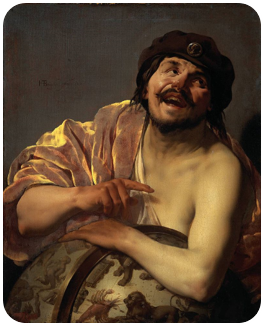
\includegraphics[width=3cm]{DEMOCRITUS}
		\captionof{figure}{Democritus (460 - 370,Hy Lạp)\label{fig:Democritus} }
\end{center}
\end{minipage}

\begin{center}
	\includegraphics[width=12cm]{Historyatom}
	\captionof{figure}{Lịch sử phát triển mô hình nguyên tử \label{fig:Historyatom} }
\end{center}
\end{hoplythuyet}
\subsubsection{Thành phần và cấu trúc của nguyên tử}
\paragraph{Thành phần}
\begin{hoplythuyet}
	Nguyên tử gồm hạt nhân chứa proton, neutron và vỏ nguyên tử chứa electron.
	\begin{center}
		\includegraphics[width=9cm]{mohinhnguyentu}
		\captionof{figure}{Mô hình nguyên tử}
	\end{center}
\end{hoplythuyet}
\paragraph{Sự tìm ra electron}
\ntd{Thí nghiệm khám phá tia âm cực của Thomson}\\
Năm 1897, J. J. Thomson (Tôm-xơn, người Anh) thực hiện thí nghiệm phóng điện qua không khí loãng đã phát hiện ra chùm tia phát ra từ cực âm.(xem hình \ref{fig:hinh3} ) và link video bằng mã QR ở bên dưới.\\ 
\hinhphai{\begin{center}
		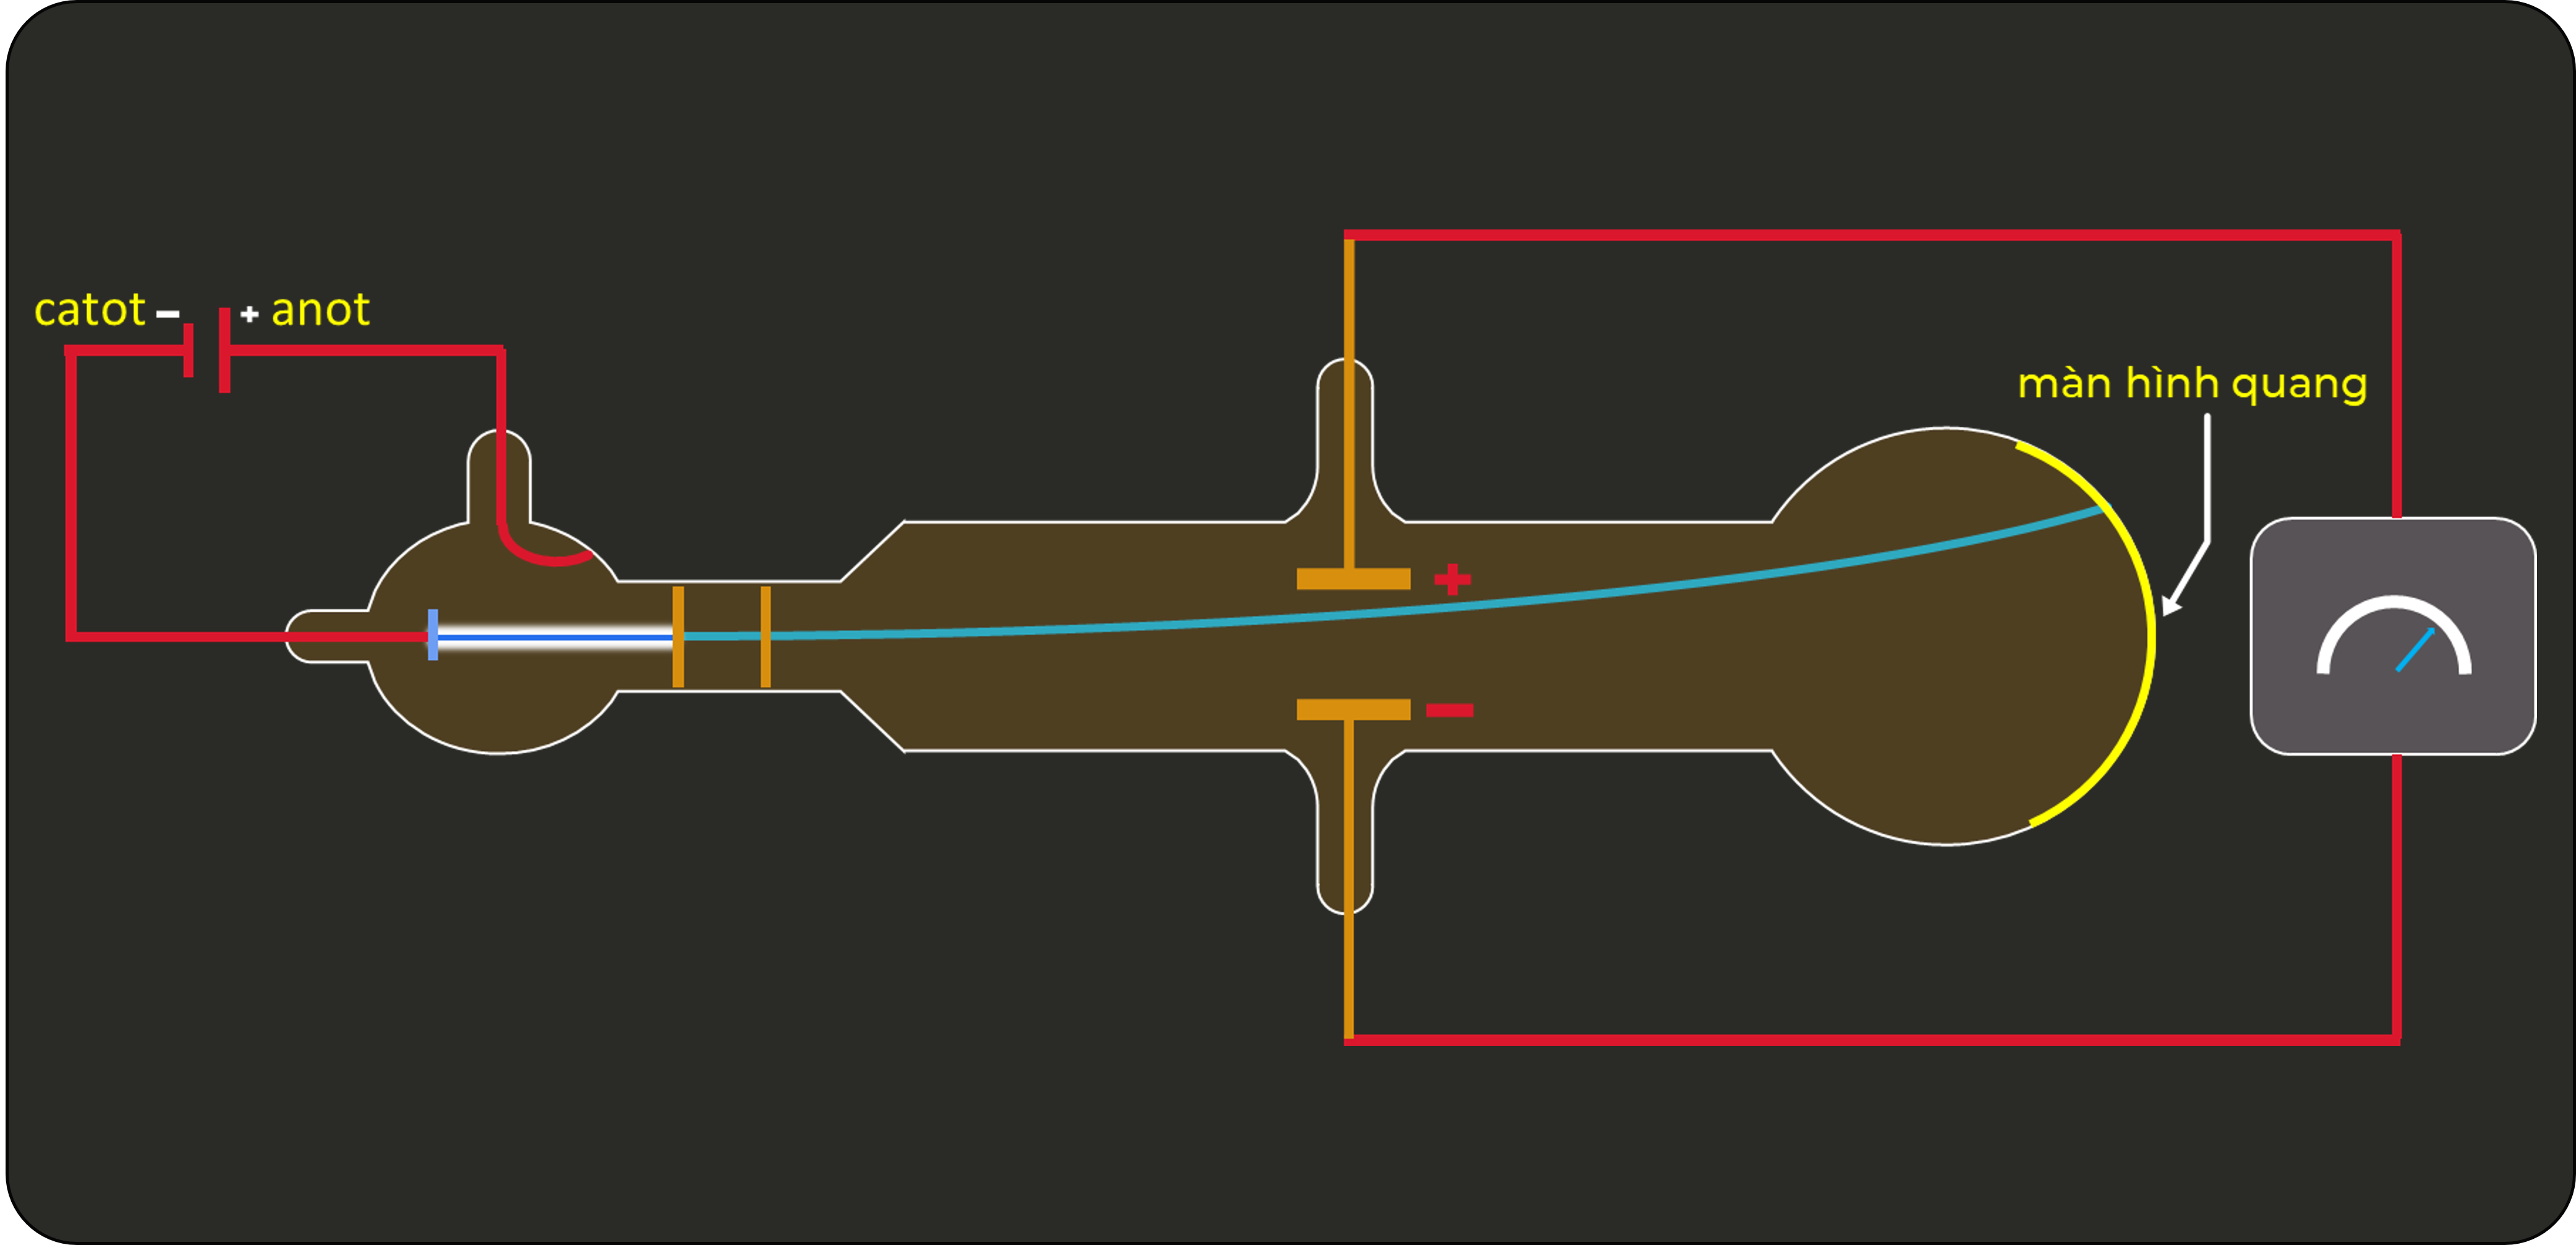
\includegraphics[width=9cm]{TNTHOMSON}\\
		\captionof{figure}{Thí nghiệm của Thomson}
		\label{fig:hinh3}
\end{center}}{\begin{tikzpicture}
\path (0,0)  node (QRCODE) {\qrcode[height=2.0cm]{https://youtu.be/y2uswXtC5O8}}
(QRCODE.south) node[anchor=north]{(\fmmfamily Các bạn  dùng ~\rotatebox{-15}{\faMobile}~quét mã QR để xem video TN nhé!)}
;
\end{tikzpicture}}
	





\begin{hoivadap}
	Vai trò của lớp bột huỳnh quang trong thí nghiệm ở hình \ref{fig:hinh3}
	\huongdan{\taodongke{10}}
\end{hoivadap}

\begin{hoivadap}
Quan sát Hình \ref{fig:hinh3} và video , giải thích vì sao tia âm cực bị hút về cực dương của trường điện.
	\huongdan{\taodongke{10}}
\end{hoivadap}

\begin{hoivadap}
	Nếu đặt một chong chóng nhẹ trên đường đi của tia âm cực thì chong chóng sẽ quay. Từ hiện tượng đó, hãy nêu kết luận về tính chất của tia âm cực.
	\huongdan{\taodongke{5}}
\end{hoivadap}
\newpage
\vspace*{6pt}
\begin{emcobiet}
	 Mô hình Thomson còn gọi là mô hình \lq\lq bánh pudding mận".Theo Thomson:
	\begin{enumerate}
		\item Nguyên tử là quả cầu mang điện tích dương, bên trong chứa các êlectron.
	    \item Nguyên tử trung hòa về điện.
	\end{enumerate}

\end{emcobiet}


\paragraph{Sự khám phá hạt nhân nguyên tử}
\ntd{Tìm hiểu thí nghiệm của Rutherford}\\
Năm 1911, E. Rutherford (Ro-dơ-pho, người Niu Di-lân) thực hiện thí nghiệm bắn phá lá vàng rất mỏng bằng chùm hạt $ \alpha $ \footnote{Hạt $\alpha$ : hạt nhân helium, mang điện tích dương.} (xem hình \ref{fig:hinh4})
\begin{center}
		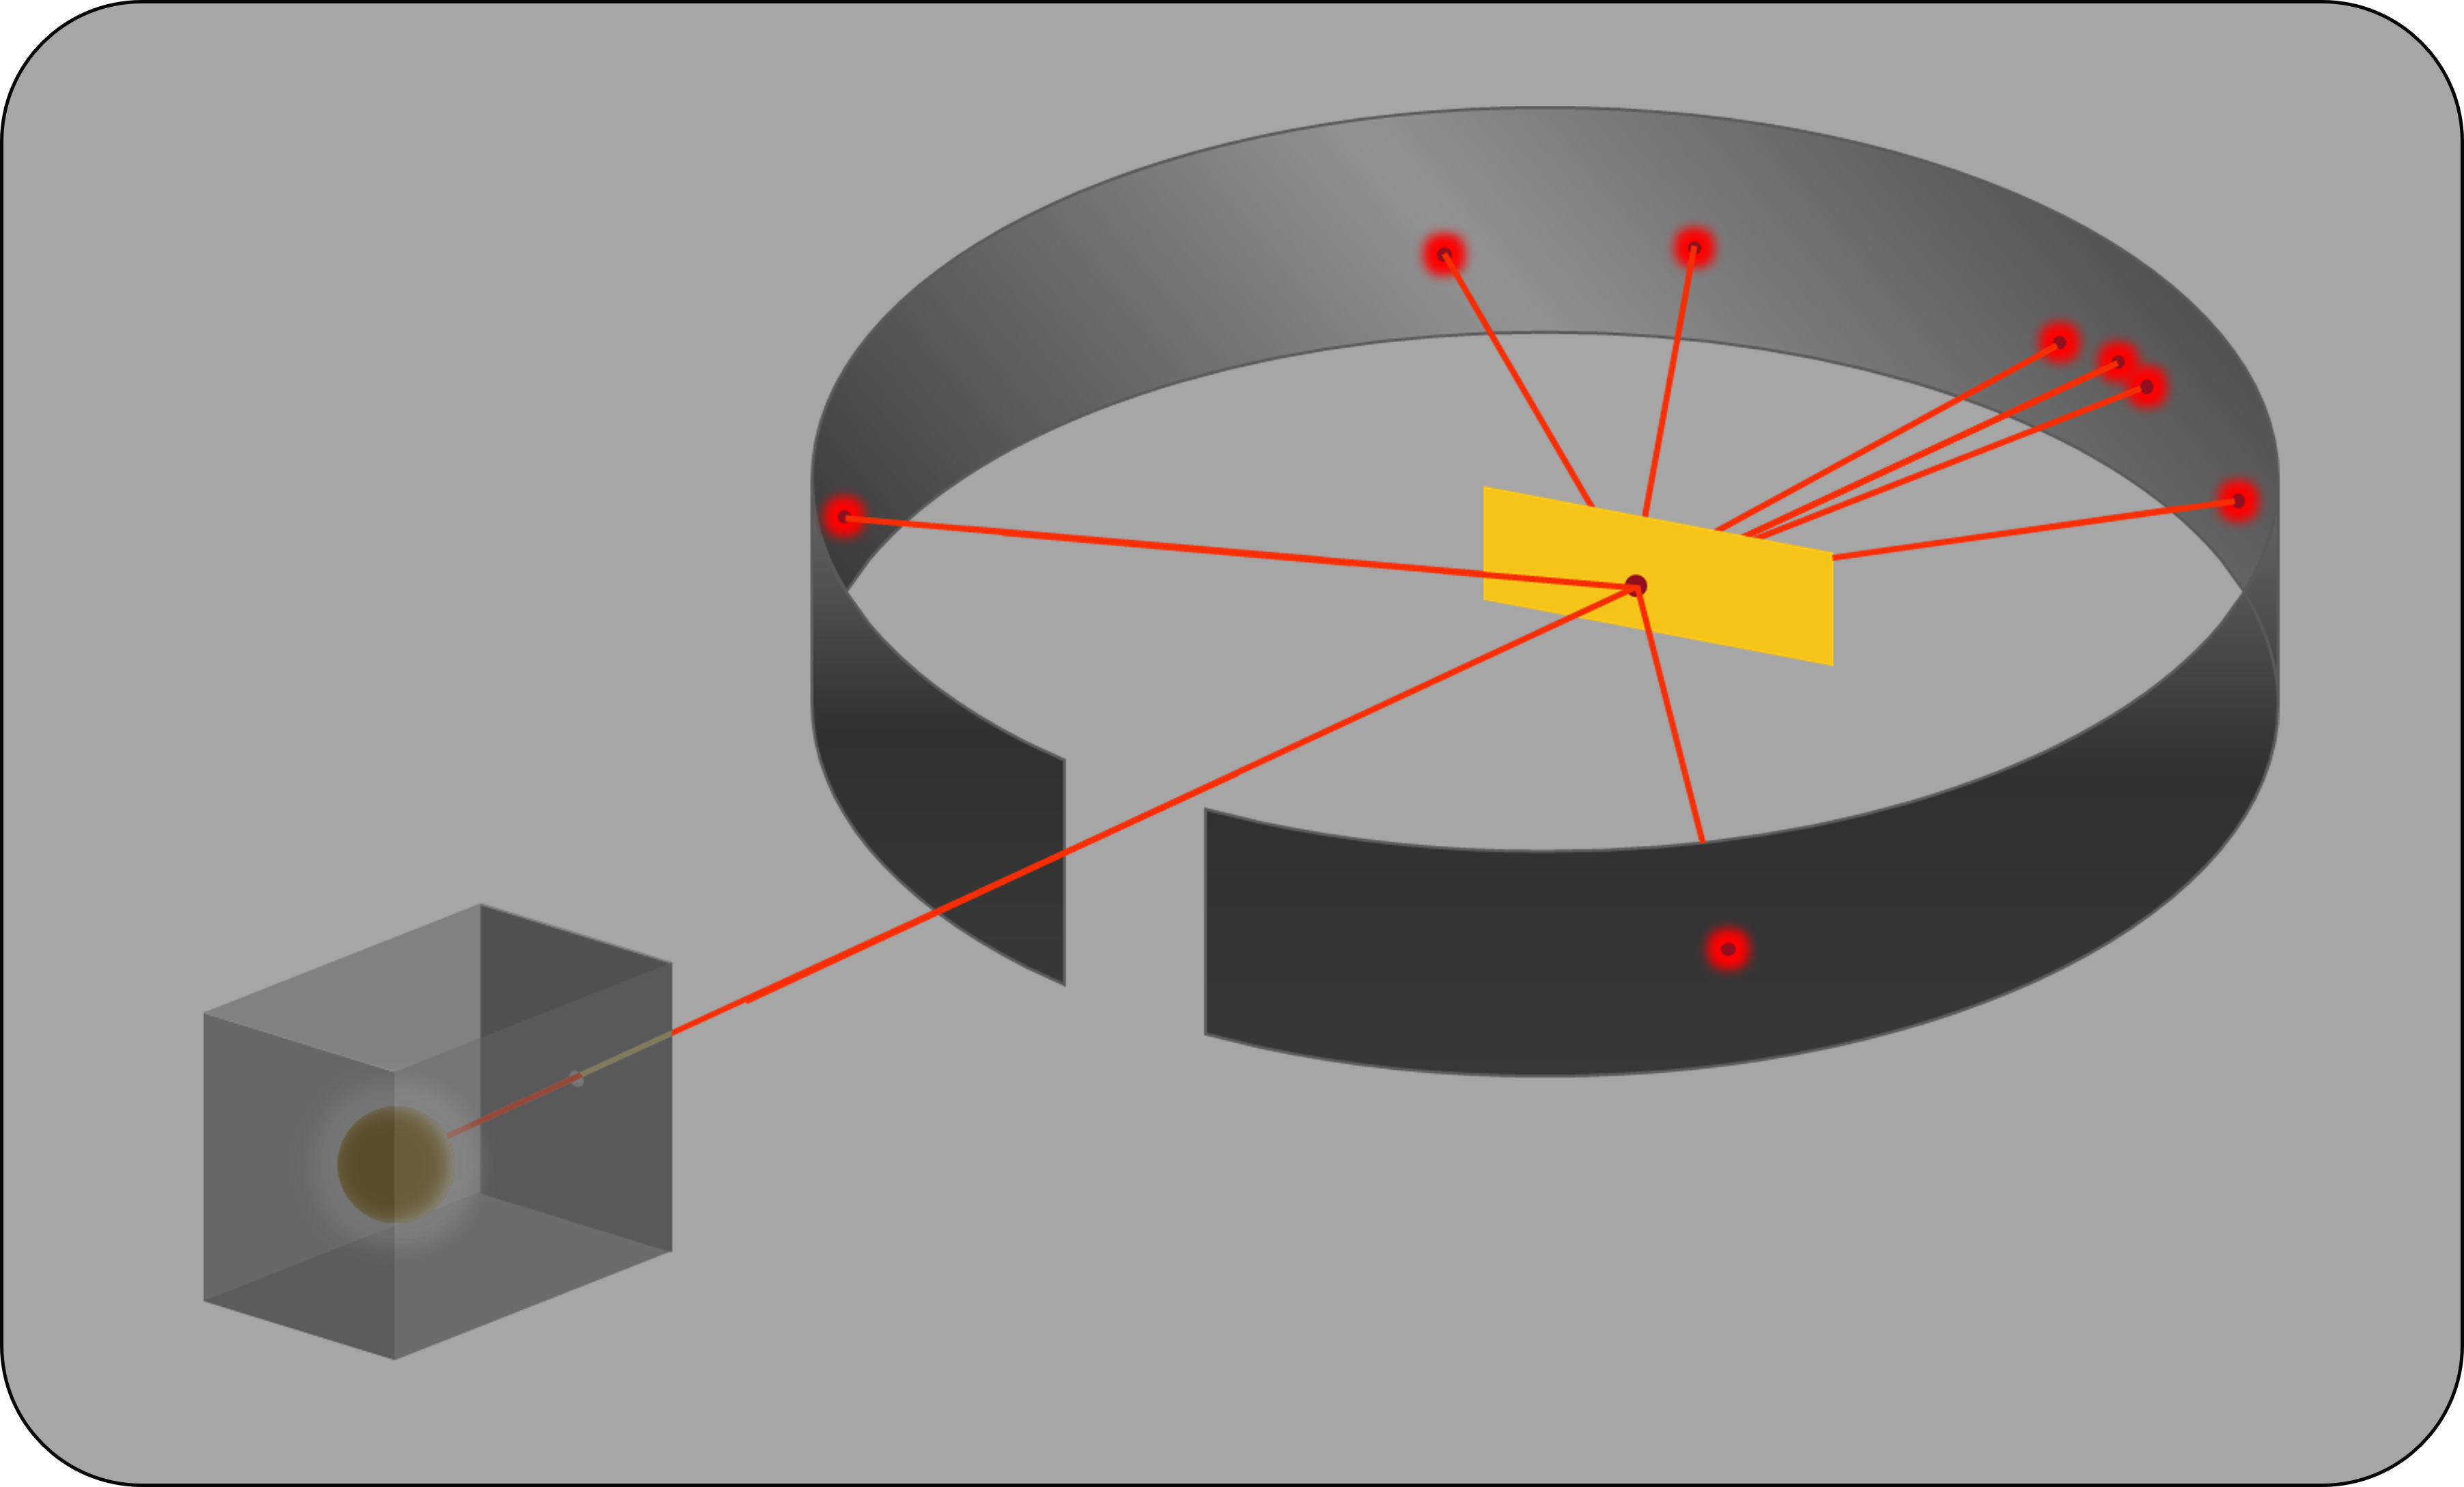
\includegraphics[width=9cm]{TNRUTHERFORT}\\
		\captionof{figure}{Thí nghiệm của Rutherford}
		\label{fig:hinh4}
\end{center}

\begin{center}
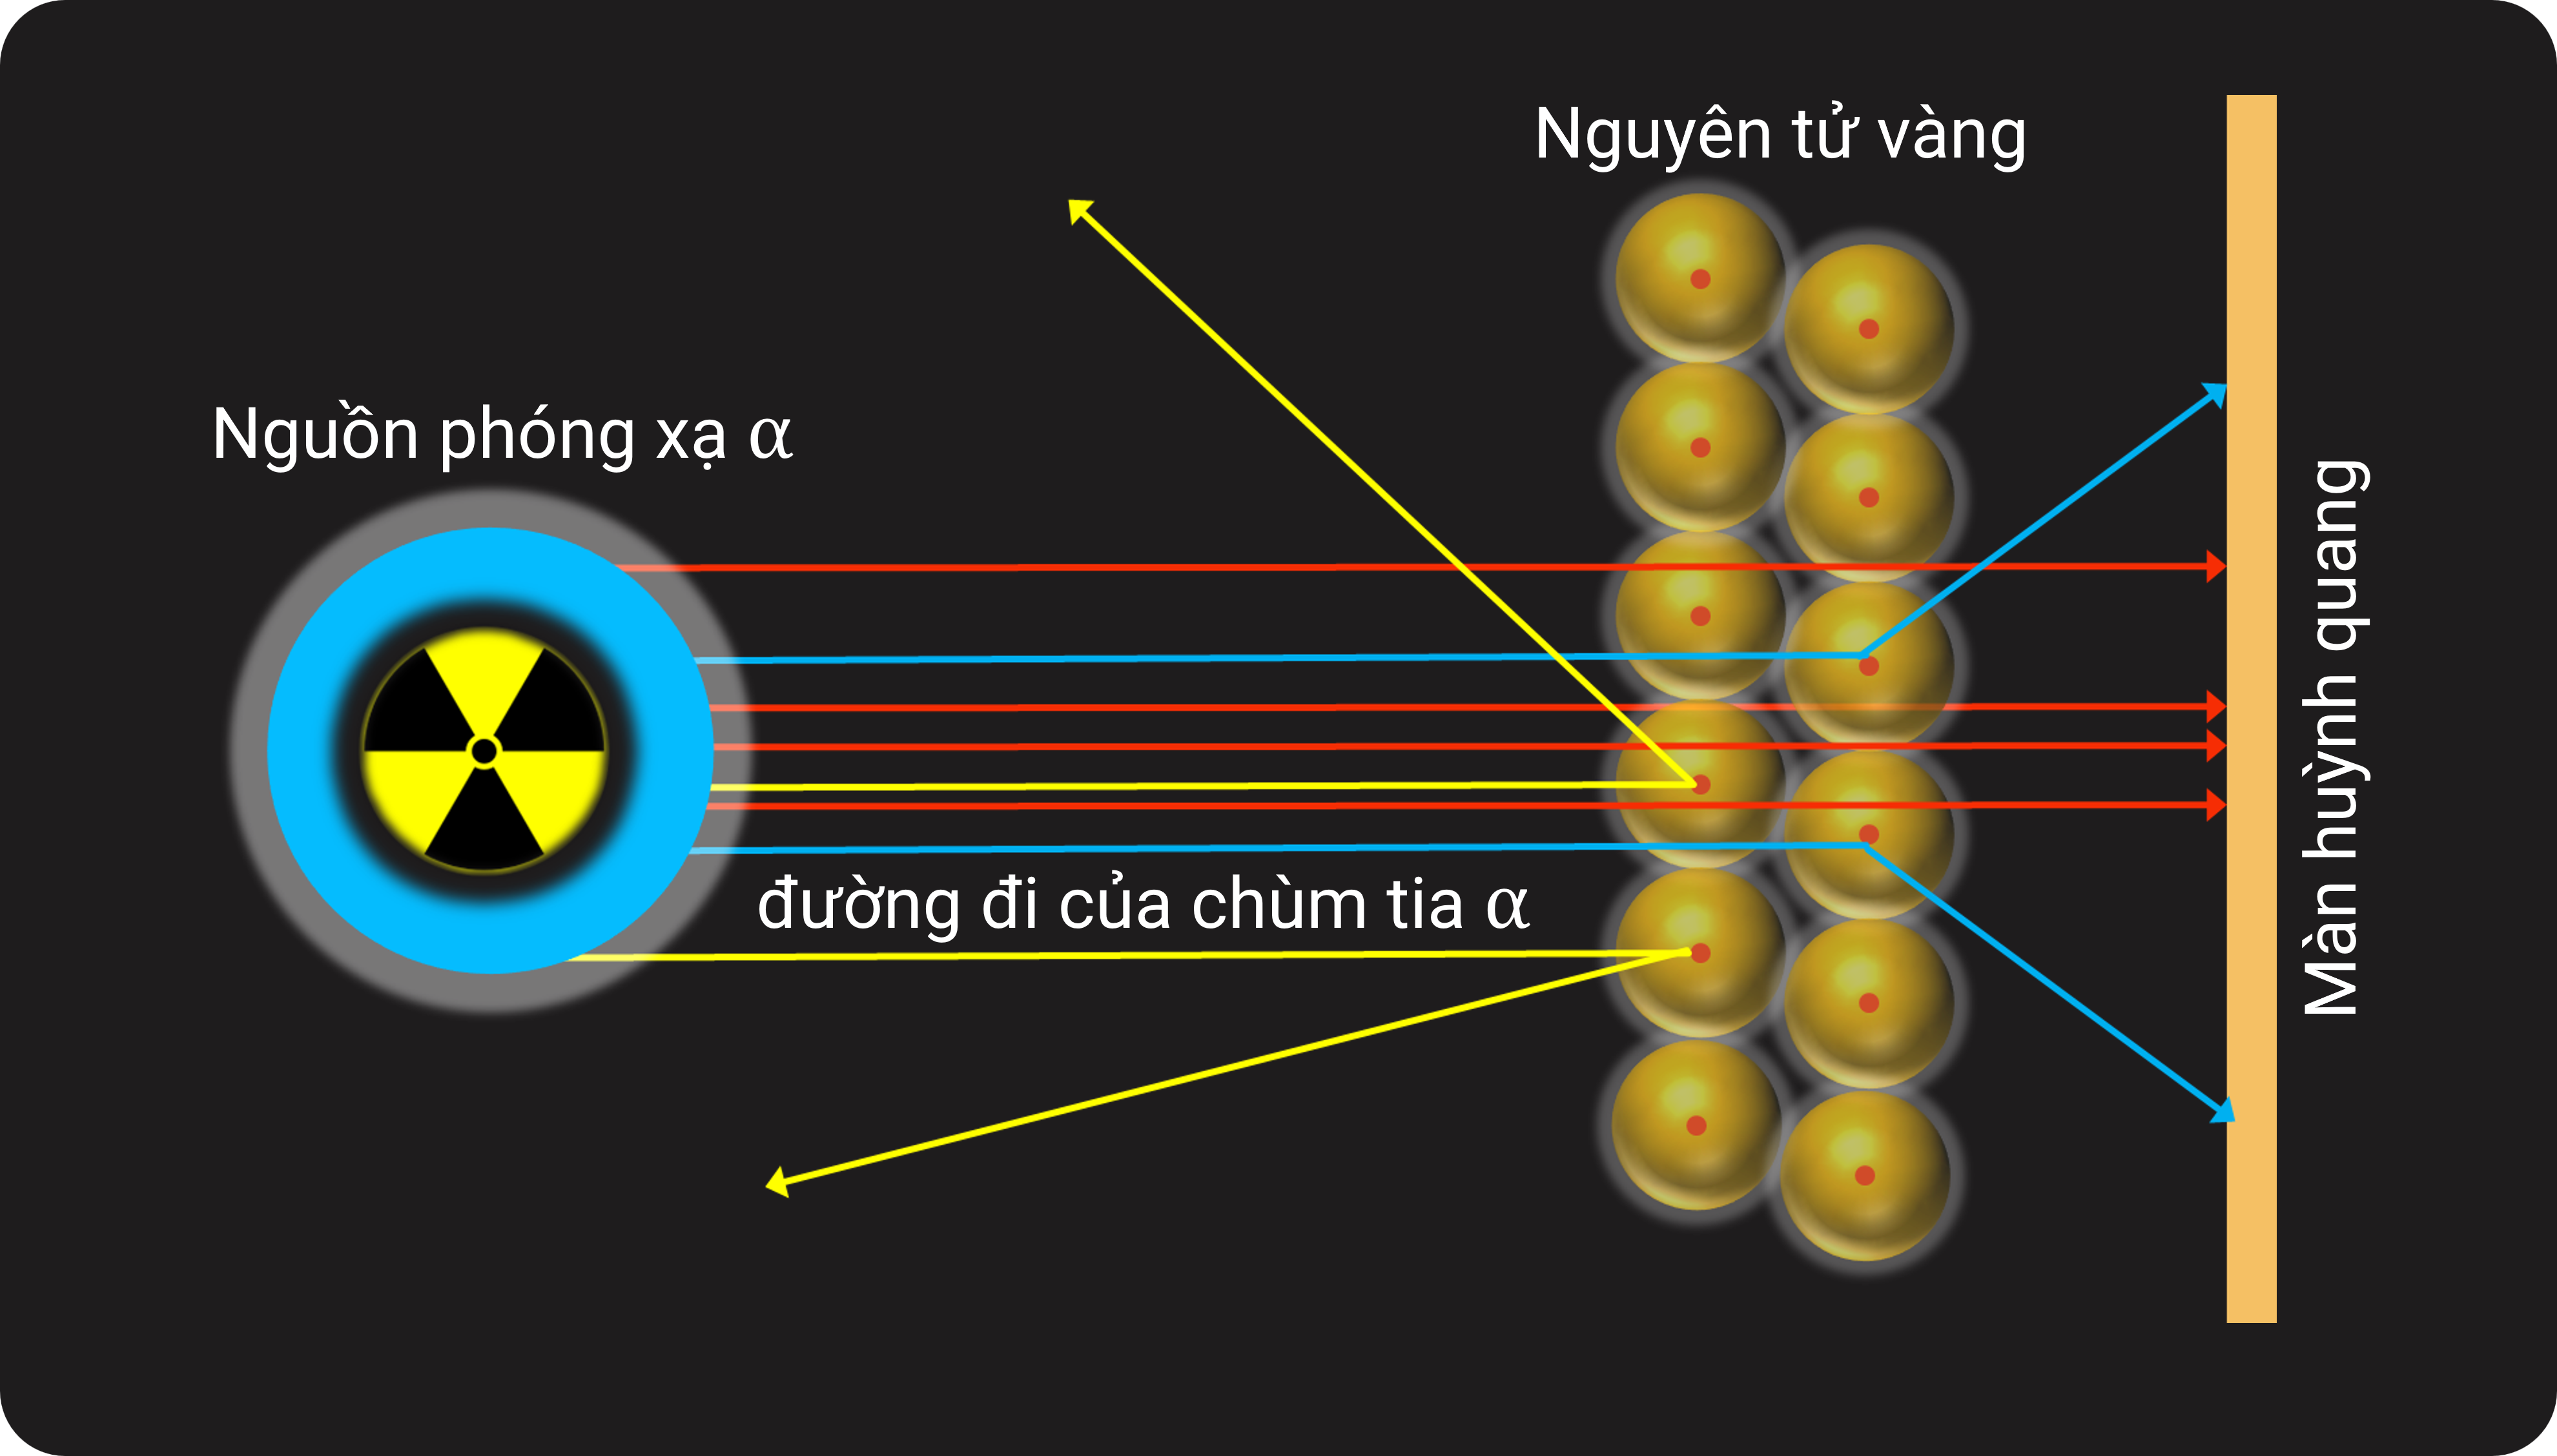
\includegraphics[width=9cm]{KQTN}\\
\captionof{figure}{Kết quả thí nghiệm của Rutherford}
\label{fig:hinh5}
\end{center}

\begin{hoivadap}
	Quan sát hình \ref{fig:hinh4}, cho biết các hạt $\alpha$ có đường đi như thế nào. Dựa vào Hình \ref{fig:hinh5} , giải thich kết quả thí nghiệm thu được.
	\huongdan{\taodongke{5}}
\end{hoivadap}
\vspace*{6pt}
\begin{hoplythuyet}
	{\bfseries{Kết luận}}
	\begin{itemize}
	\item Nguyên tử có cấu tạo rỗng, gồm hạt nhân ở trung tâm và lớp vỏ là các electron chuyển động xung quanh hạt nhân.
	\item Nguyên tử trung hoà về điện: số đơn vị điện tích dương của hạt nhân bằng số đơn vị điện tích âm của các electron trong nguyên tử.
	\end{itemize}
\end{hoplythuyet}
\paragraph{Cấu tạo hạt nhân nguyên tử}
\begin{center}
	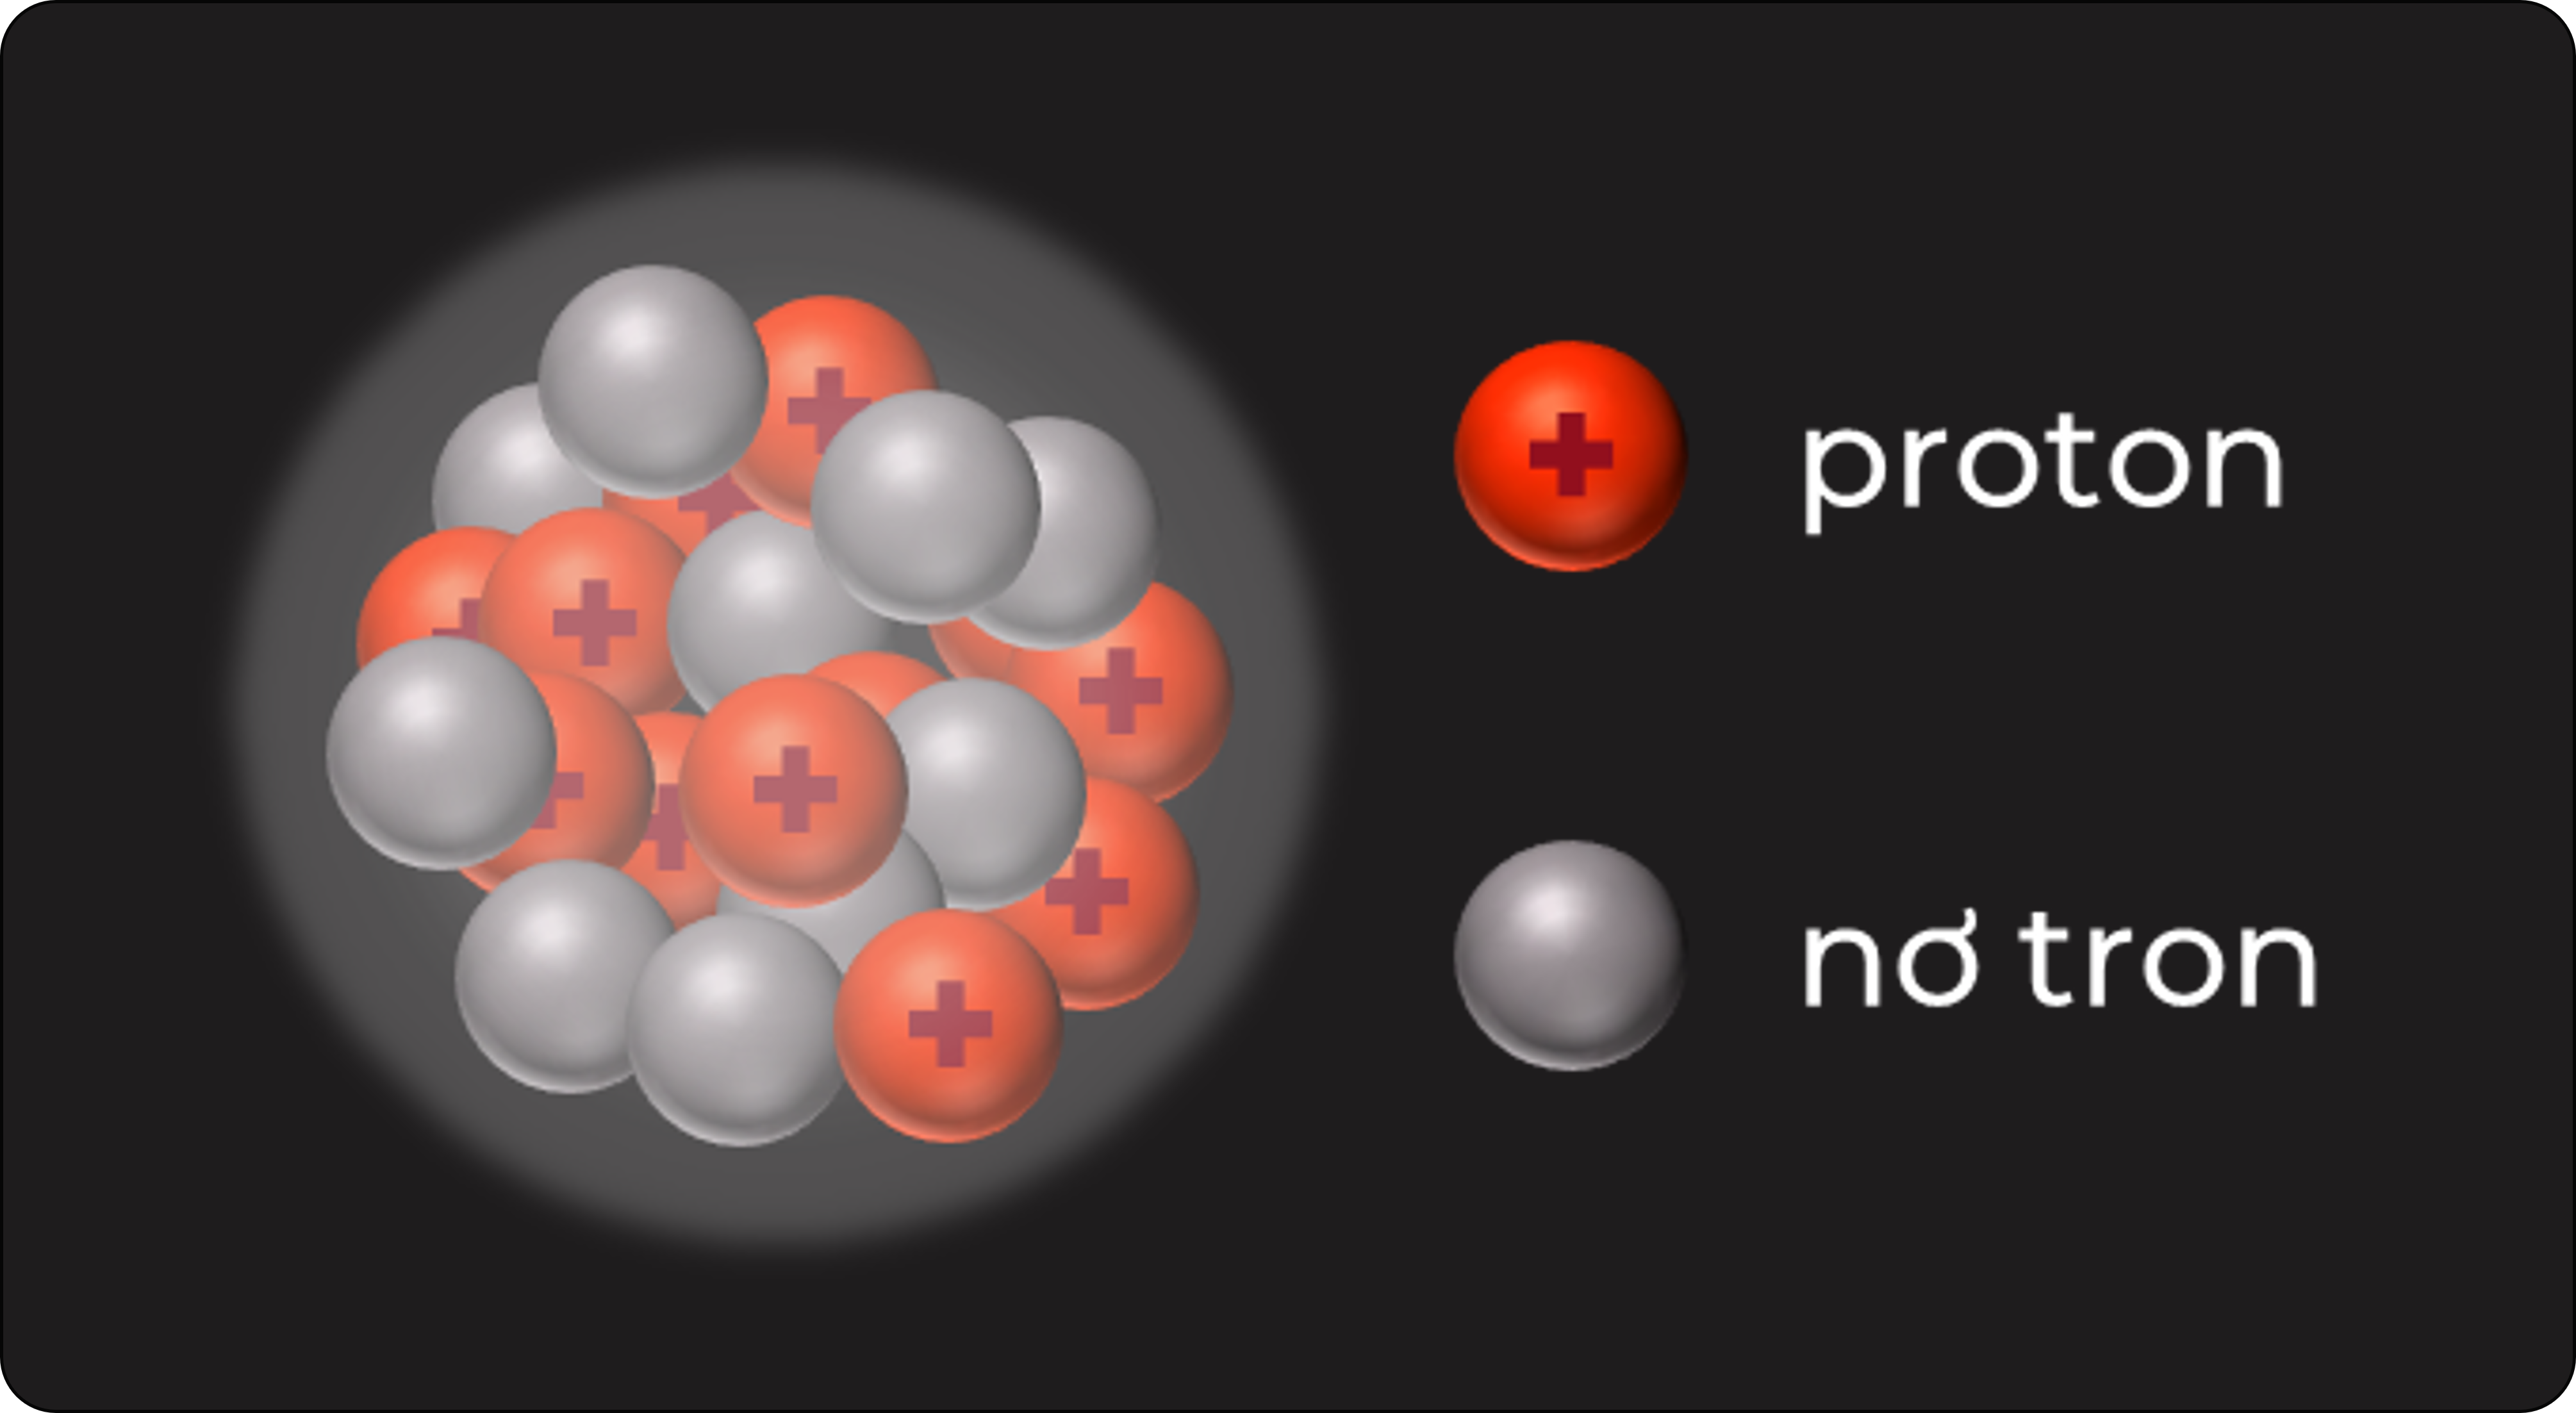
\includegraphics[width=9cm]{CAUTAOHATNHAN}\\
	\captionof{figure}{Thành phần của hạt nhân}
	\label{fig:hinh6}
\end{center}
\begin{hoivadap}
	Quan sát hình \ref{fig:hinh6} và kết hợp SGK , các bạn hãy nêu thành phần của hạt nhân
\end{hoivadap}
\begin{hoplythuyet}
	Proton, neutron và electron là các hạt cấu tạo nên nguyên tử.
\end{hoplythuyet}
\begin{tongket}
	Thành phần cấu tạo của nguyên tử gồm:
\begin{itemize}
	\item  Hạt nhân (nucleus): ở tâm của nguyên tử, chứa các proton mang điện tích dương và các neutron không mang điện.
	\item Vỏ nguyên tử: chứa các electron mang điện tích âm, chuyển động rất nhanh xung quanh hạt nhân.
	\item Trong nguyên tử, số proton bằng số electron nên nguyên tử trung hoà điện.
	\item Khối lượng của electron rất nhỏ, không đáng kể so với khối lượng của proton hay neutron nên khối lượng của nguyên tử tập trung hầu hết ở hạt nhân.
\end{itemize}
\end{tongket}


\begin{longtable}{|c|c|c|c|c|c|}
		\caption{\indam[dndo]{Khối lượng, điện tích của các loại hạt cấu tạo nên nguyên tử}}
		\label{tab:table1}\\
\hline
\rowcolor{dnxanh!25} \indam[dnxanh]{Hạt} & \indam[dnxanh]{Kí hiệu} & $\begin{array}{c}\text {\indam[dnxanh]{Khối lượng} } \\
		\text {\indam[dnxanh]{(kg)}  }\end{array}$ & \indam[dnxanh]{Khối lượng (amu)} & $\begin{array}{c}\text { \indam[dnxanh]{Điện tích} } \\
		\text { \indam[dnxanh]{(C)} }\end{array}$ & $\begin{array}{l}\text { \indam[dnxanh]{Điện tích} } \\
		\text { \indam[dnxanh]{tương đối} }\end{array}$ \\
\hline\endhead
\rowcolor{dnvang!15} Proton & $p$ & $1,672 \cdot 10^{-27}$ & $\approx 1$ & $1,602 \cdot 10^{-19}$ & +1 \\
\hline
\rowcolor{dnvang!15} Neutron & $\mathrm{n}$ & $1,675 \cdot 10^{-27}$ & $\approx 1$ & 0 & 0 \\
\hline\rowcolor{dnvang!15} Electron & e & $9,109 \cdot 10^{-31}$ & $\begin{array}{c}
		~ \\
		\dfrac{1}{1837} \approx 0,00055\\
		~ \\
	\end{array}$ & $-1,602 \cdot 10^{-19}$ & -1 \\
	\hline
	\end{longtable}
\paragraph{KíCH THƯỚC VÀ KHỐI LƯợNG NGUYÊN TỬ}
\begin{center}
	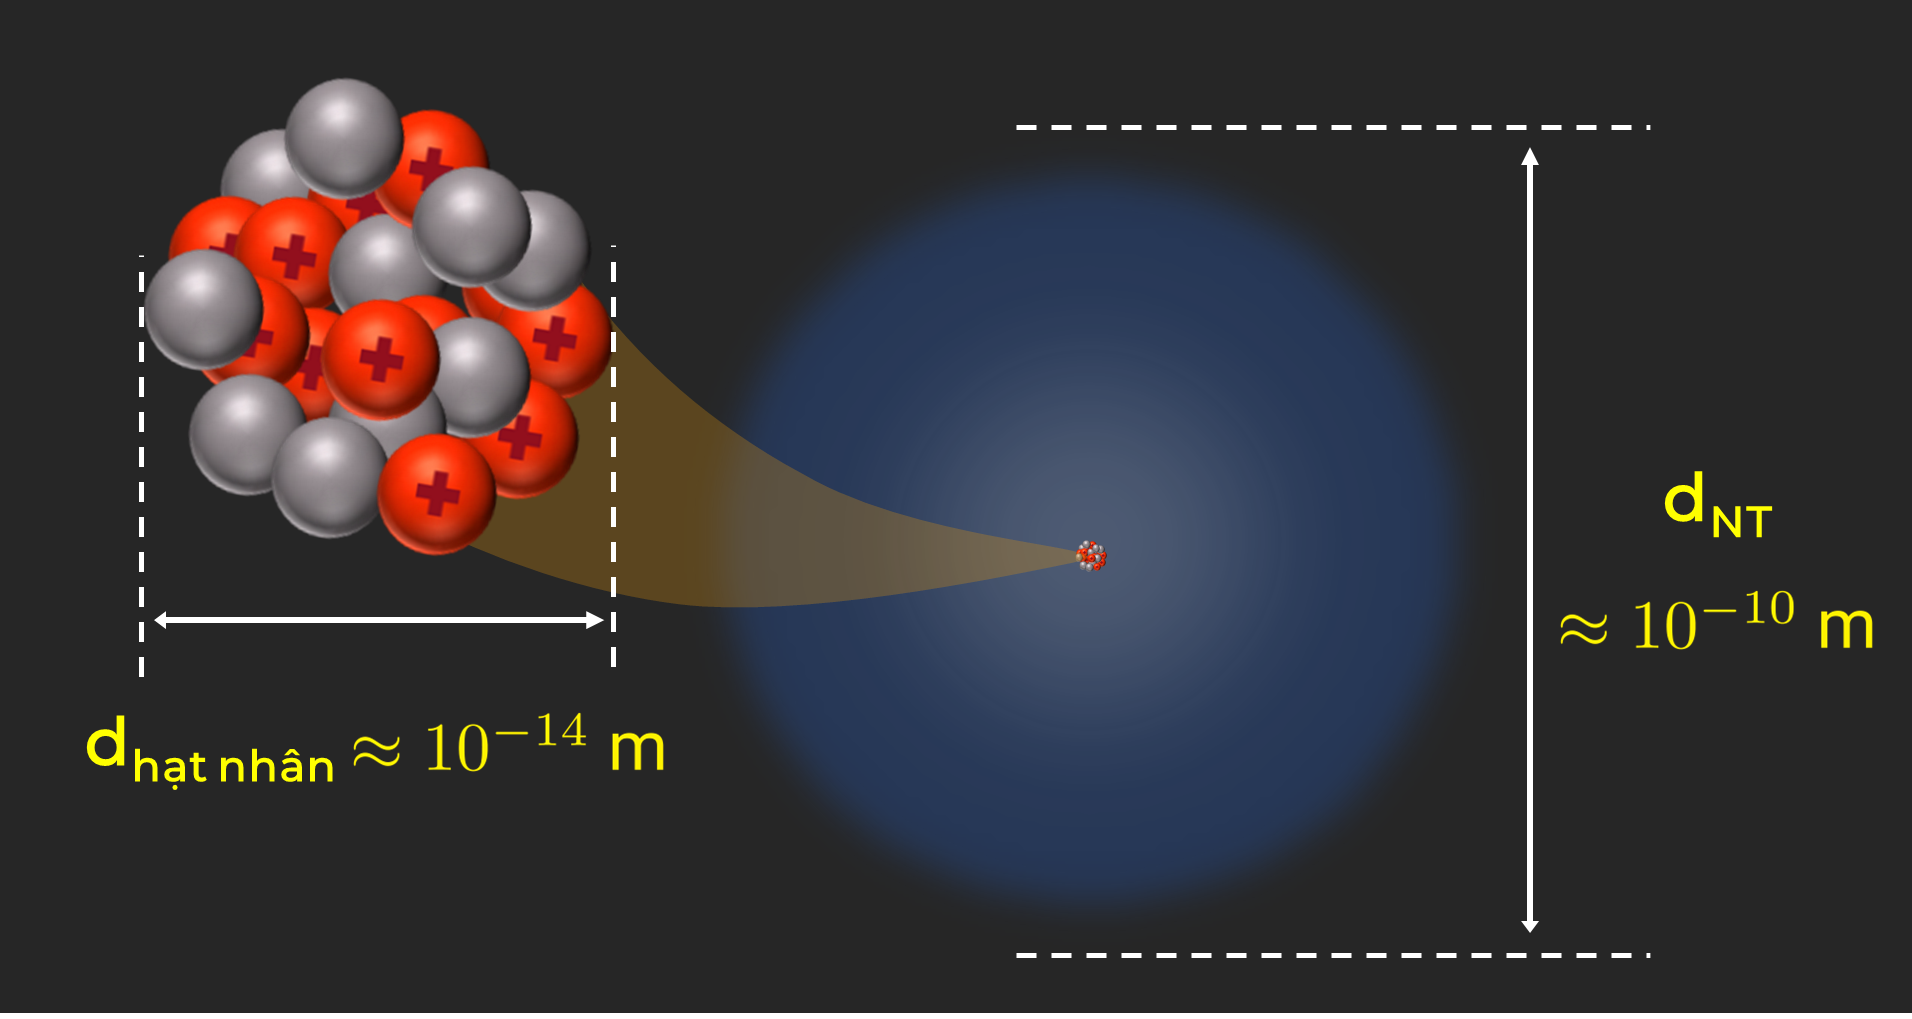
\includegraphics[width=9cm]{ktnt}\\
	\captionof{figure}{So sánh kích thước hạt nhân , nguyên tử}
	\label{fig:hinh7}
\end{center}
\begin{notegsnd}
		\begin{itemize}
\item Đơn vị kích thước thường dùng của nguyên tử là Angstron ($ A^0 $) hoặc nano mét (nm)			
	$$1 \mathrm{~nm}=10^{-9}~\mathrm{m} ; 1 A^0=10^{-10}~\mathrm{~m} ; 1 \mathrm{~nm}=10 A^0; 1 A^0=10^{2}~\mathrm{pm}$$
	\begin{center}
	\tcbox[width=5cm,colframe=dndo]{$ \dfrac{d_{\text{NT}}}{d_{\text{hạt nhân}}}\approx \dfrac{10^{-10}}{10^{-14}} \approx 10^4~\mathrm{\text{lần}} $}
	\end{center}
		\item Đơn vị của khối lương nguyên tử là amu (atomic mass unit),
		$$
		1 \mathrm{amu}=1,6605 \times 10^{-27} \mathrm{~kg} \text {. }
		$$
		\item Đơn vi của điện tích các hạt cơ bản là $\mathrm{e}_0$ (điện tích nguyên tố),
		$$
		1 \mathrm{e}_0=1,602 \times 10^{-19} \mathrm{C} \text {. }
		$$
	\end{itemize}
\end{notegsnd}
\newpage
\vspace*{3pt}

\ntd{BÀI TẬP TRẮC NGHIỆM}:
\begin{dangntd}{LÝ THUYẾT VỀ CẤU TẠO NGUYÊN TỬ}
\giaibaitap{Phương pháp giải}
\begin{itemize}
	\item Nắm vững về cấu tạo nguyên tử
	\item Nắm vững kết quả thí nghiệm của Thomson,Rutherford
\end{itemize}
\end{dangntd}
\Opensolutionfile{ansbook}[DAPAN/BTTLH10CO102tachLG]
\Opensolutionfile{ans}[DAPAN/BTTLH10CO102]
\begin{ex}[1]
	Các hạt cơ bản của hầu hết các nguyên tử là?
	\choice
{%
electron
}
{%
	electron và proton
}
{%
 proton và notron
}
{%
\True electron, proton và notron
}
%\sodongkeex[5]
\huongdan{

}
\end{ex}


\begin{ex}[1]
	Hạt nhân của hầu hết các nguyên tử gồm có?
	\choice
	{%
		electron
	}
	{%
		electron và proton
	}
	{%
	\True proton và notron
	}
	{%
		 electron, proton và notron
	}
%\sodongkeex[5]
\huongdan{
	
}
\end{ex}

\begin{ex}[2]
Trong thí nghiệm của Thomson, phát biểu nào sau đây sai với kết quả thí nghiệm ta quan sát được?
	\choice
{%
 Tia âm cực là các chùm hạt electron di chuyển từ cực âm sang cực dương
}
{%
	Tia âm cực là chùm hạt mang điện tích âm
}
{%
\True	Tia âm cực bị lệch về phía bản cực âm của nguồn điện
}
{%
	Tia âm cực bị lệch hướng khi ta đặt nó trong từ trường
}
%\sodongkeex[5]
\huongdan{
	
}
\end{ex}

\begin{ex}[2]
Theo mô hình bánh pudding mận của Thomson, phát biểu nào sau đây là đúng?
\choice
{%
Nguyên tử có cấu tạo rỗng gồm hạt nhân mang điện tích dương và vỏ là các electron chuyển động xung quanh hạt nhân.
}
{%
Nguyên tử có cấu tạo rỗng gồm hạt nhân mang điện tích dương và vỏ là các electron chuyển dộng xung quanh hạt nhân theo những quỹ đạo có kích thước và năng lượng cố định
}
{%
\True	nguyên tử bao gồm các electron nằm rải rác trong một đám mây hình cầu mang điện tích dương.
}
{%
	các electron  quay quanh hạt nhân không theo một quỹ đạo xác định, mà chúng tạo thành các đám mây điện tích mà tại đó xác suất tìm thấy electron là lớn nhất
}
%\sodongkeex[5]
\huongdan{
	
}
\end{ex}
\begin{ex}[2]
Cho các phát biểu sau:
\begin{enumerate}[(1)]
\item Tất cả các hạt nhân nguyên tử đều được cấu tạo từ các hạt proton và neutron.
\item Khối lượng nguyên tử tập trung phần lớn ở lớp vỏ.
\item Trong nguyên tử, số electron bằng số proton.
\item Trong hạt nhân nguyên tử, hạt mang điện là proton và electron.
\item Trong nguyên tử, hạt electron có khối lượng không đáng kể so với các hạt còn lại.
\end{enumerate}
Số phát biểu đúng là
\choice
{%
	1
}
{%
\True 2
}
{%
3
}
{%
4
}
\huongdan{%
Phát biểu đúng là:
Trong hạt nhân nguyên tử, hạt mang điện là proton và electron.\\
Trong nguyên tử, hạt electron có khối lượng không đáng kể so với các hạt còn lại
}

\end{ex}

\begin{ex}[2]
Điều nào sau đây đúng theo mô hình nguyên tử của Thomson?
\choice
{%
Nguyên tử không trung hòa về điện
}
{%
\True Nguyên tử là quả cầu mang điện tích dương có chứa các êlectron bên trong
}
{%
Điện tích âm và điện tích dương trong nguyên tử có độ lớn bằng nhau
}
 {%
 Không có điều nào ở trên
 }
%\sodongkeex[5]
\huongdan{
	
}
\end{ex}


\begin{ex}[3]
	Trong hiện tượng xả điện qua khí ở áp suất thấp, sự tỏa sáng màu trong ống xuất hiện là kết quả của:
	\choice
	{% 
\True va chạm giữa các hạt mang điện được phát ra từ cực âm và nguyên tử của khí
	}
{% 
	va chạm giữa các electron khác nhau của các nguyên tử trong khí
}
{% 
	kích thích các electron trong các nguyên tử
}	
{% 
va chạm giữa các nguyên tử của khí
}	
%\sodongkeex[5]
\huongdan{
	
}	
\end{ex}

\begin{ex}[2]
Mô hình đầu tiên về nguyên tử được đưa ra bởi:
\choice
{%
N. Bohr
}
{% 
	E. Goldstein
}
{% 
	Rutherford
}
{% 	
\True J.J. Thomson
}
%\sodongkeex[5]
\huongdan{
	
}
\end{ex}

\begin{ex}[2]
Nếu đường kính của nguyên tử khoảng $10^2 \mathrm{pm}$ thì đường kính của hạt nhân khoảng
\choice
{%
$10^2 \mathrm{pm}$
}
{%
$10^{-4} \mathrm{pm}$
}
{%
\True	$10^{-2} \mathrm{pm}$
}
{
$10^4 \mathrm{pm}$
}
%\sodongkeex[5]
\huongdan{
	
}
\end{ex}
\Closesolutionfile{ans}
\Closesolutionfile{ansbook}


\newpage
\giaibaitap{BÀI TẬP TỰ LUẬN}
\Opensolutionfile{ansbt}[DAPAN/BT_H10C0102]
\begin{btex}[2]
	Trong thí nghiệm của Rutherford, khi sử dụng các hạt alpha (ion $\mathrm{He}^{2+}$, kí hiệu là $\mathrm{a}$ ) bắn vào lá vàng thì:
	\begin{itemize}
	\item Hầu hết các hạt a xuyên thẳng qua lá vàng.
	\item Một số ít hạt a bị lệch quỹ đạo so với ban đầu.
	\item Một số rất ít hạt a bị bật ngược trở lại.
	\end{itemize}
	Từ kết quả này, em có nhận xét gì về cấu tạo nguyên tử?
	\loigiai{
	Trong thí nghiệm của Rutherford, khi sử dụng các hạt alpha (ion $\mathrm{He}^{2+}$, kí hiệu là a) bắn vào lá vàng thì:
	\begin{itemize}
	\item Hầu hết các hạt a xuyên thẳng qua lá vàng chứng tỏ nguyên tử có cấu tạo rỗng.
	\item Một số ít hạt a bị lệch quỹ đạo so với ban đầu chứng tỏ hạt nhân nguyên tử cùng điện tích dương như hạt hạt alpha (ion $\mathrm{He}^{2+}$, kí hiệu là $ \alpha $).
	\item Một số rất ít hạt a bị bật ngược trở lại chứng tỏ kích thước hạt nhân nhỏ hơn rất nhiều so với kích thước của nguyên tử và khối lượng nguyên tử tập trung chủ yếu ở hạt nhân.
	\end{itemize}

}
\end{btex}

\begin{btex}[2]
Viết lại bảng sau vào vở và điền thông tin còn thiếu vào các ô trống:\\
\begin{tabular}{|c|c|c|c|c|c|c|}
\rowcolor{dnxanh!25} 
\hline \indam[dnxanhdam]{Nguyên tố} & \indam[dnxanhdam]{Kí hiệu} & \color{dnxanhdam} {$\mathbf{Z}$} & \indam[dnxanhdam]{Số e} & \indam[dnxanhdam]{Số p} & \indam[dnxanhdam]{Số n} & \indam[dnxanhdam]{Số khối} \\
\rowcolor{dnvang!25} 
\hline \indam[dnxanhdam]{Carbon} & $\mathrm{C}$ & 6 & 6 & $?$ & 6 & $?$ \\
\rowcolor{dnvang!25} 
\hline \indam[dnxanhdam]{Nitrogen} & $\mathrm{N}$ & 7 & $?$ & 7 & $?$ & 14 \\
\rowcolor{dnvang!25} 
\hline \indam[dnxanhdam]{Oxygen} & $\mathrm{O}$ & 8 & 8 & $?$ & 8 & $?$ \\
\rowcolor{dnvang!25} 
\hline \indam[dnxanhdam]{Sodium (natri)} & $\mathrm{Na}$ & 11 & $?$ & 11 & $?$ & 23 \\
\rowcolor{dnvang!25}
\hline \indam[dnxanhdam]{Aluminium (nhôm)} & $\mathrm{Al}$ & $?$ & 13 & $?$ & $?$ & 27 \\
\hline
\end{tabular}
\huongdan{
\taodongke{5}
}
\end{btex}

\Closesolutionfile{ansbt}










\newpage
\begin{dangntd}{Bài tập về khối lượng, kích thước nguyên tử}	
	\giaibaitap{Phương pháp giải}\\
	\tieumuc{Các công thức liên quan khối lượng}
	\begin{itemize}
		\item $ m _{\text{nguyên tử}=m_{p}+m_{n} + m_{e} } $ (tính chính xác); $ m _{\text{nguyên tử}} \approx  m_{p} + m_{n} \approx m_{\text{hạt nhân}} $ (tính gần đúng)
		\item Khối lượng tính ra kg của 1 nguyên tử carbon-12 là $ 19,926 . 10^{27}~\mathrm{kg}$.
		\item 1 amu được định nghĩa bằng $\dfrac{1}{12}$ khối lượng 1 nguyên tử carbon-12:
		\item$1 \mathrm{amu}=\dfrac{19,926 \cdot 10^{-27} \mathrm{~kg}}{12}=1,661 \cdot 10^{-27} \mathrm{~kg}$
		\item$1 \mathrm{mol}$ chứa $ 6,02.10^{23} $ nguyên tử, phân tử, ion.
	\end{itemize}
	\tieumuc{Các công thức liên quan kích thước}
	\begin{itemize}
		\item Thể tích của hình cầu:
		$ V=\dfrac{4}{3}\pi r^3 $
		\item Phần trăm thể tích các nguyên tử trong tinh thể $ = \dfrac{V_{\text{các nguyên tử}}}{V_{\text{tinh thể}}}\cdot 100\% $
		\item Một số đơn vị đo: 
		$\left\{\begin{array}{l}
			1~\mathrm{nm} = 10^{-9}~\mathrm{m}\\
			1~\mathrm{A^{0}} = 10^{-10}~\mathrm{m}\\
			1~\mathrm{pm} = 10^{-12}~\mathrm{m}	
		\end{array}\right.$
	\end{itemize}
\end{dangntd}
\begin{vdm}{Ví dụ mẫu}
\end{vdm}

%Câu 1: Khối lượng của nguyên tử magnesium là $39,8271 \cdot 10^{-27} \mathrm{~kg}$. Khối lượng của magnesium theo amu là
%A. 23,978
%B. $66,133 \cdot 10^{-51}$.
%C. 24,000 .
%D. $23,985 \cdot 10^{-3}$.

\begin{vdex}[2]	
	Khối lượng của nguyên tử magnesium là $39,8271 \cdot 10^{-27} \mathrm{~kg}$. Khối lượng của magnesium theo amu là
	\choice
	{%
		\True $ 23,978 $
	}
	{%
		$66,133 \cdot 10^{-51}$
	}
	{%
		$23,985 \cdot 10^{-3}$
	}
	{%
		$ 24,000 $
	}
	\huongdan{
		
	}	
\end{vdex}

\begin{vdex}[2]
	Khối lượng tuyệt đối của một nguyên tử oxygen bằng $26,5595.10^{-27} \mathrm{~kg}$. Hãy tính khối lượng nguyên tử (theo amu) và khối lượng mol nguyên tử (theo g) của nguyên tử này.
	\loigiai
	{%
		$
		1 \mathrm{amu}=1,661 \cdot 10^{-27} \mathrm{~kg}
		$\\
		
		
		Khối lượng của nguyên tử oxygen theo amu là:
		$
		\dfrac{26,5595 \cdot 10^{-27}}{1,661 \cdot 10^{-27}} \approx 15,99~ \mathrm{amu}
		$\\
		
		$1 \mathrm{mol}$ chứa $ 6,02.10^{23} $ nguyên tử\\
		$\Rightarrow$ Khối lượng mol của oxygen là  $=26,5595.10^{-24}.6,02.10^{23}= 15,99~ \mathrm{gam} $
		
	}
\end{vdex}

%Câu 3: Nguyên tử helium có 2 proton, 2 neutron và 2 electron. Khối lượng của các electron chiếm baoo nhiêu $\%$ khối lượng nguyên tử helium?
%A. $2,72 \%$.
%B. $0,272 \%$.
%C. $0,0272 \%$.
%D. $0,0227 \%$.

\begin{vdex}[2]
	Nguyên tử helium có 2 proton, 2 neutron và 2 electron. Khối lượng của các electron chiếm bao nhiêu $\%$ khối lượng nguyên tử helium?
	\choice
{%
	$2,72 \%$
}
{%
	$0,272 \%$
}
{%
\True	$0,0272 \%$
}
{%
	$0,0227 \%$
}
	\huongdan
	{%
		Khối lượng nguyên tử helium là:\\ $ m_{NT} = 2m_{p} + 2m_{n} + 2m_{e} = 2.1,672.10^{-27} + 2.1,675.10^{-27} + 2 .9,109.10^{-31} = 6.696.10^{-27}~\mathrm (kg) $\\
		Phần trăm khối lượng của electron trong nguyên tử helium là:\\
		$ \%m_{e}=\dfrac{2 .9,109.10^{-31}}{5.51941.10^{-27}}.100\%=0,0272 \%$
		
	}
\end{vdex}



\begin{vdex}[2]
	Khối lượng riêng của canxi kim loại  là $ 1,55 g/cm^3 $. Giả thiết rằng , trong tinh thể canxi các nguyên tử là những hình cầu chiếm $ 74\% $ thể tích tinh thể, phần còn lại là khe rỗng.Bán kính nguyên tử tính theo lý thuyết là
	\choice
	{%
		$0,185~\mathrm{nm}$
	}
	{%
	\True	$0,196~\mathrm{nm}$
	}
	{%
		$0,155~\mathrm{nm}$
	}
	{%
		$0,168~\mathrm{nm}$
	}
	\huongdan
	{%
		Lấy 1 mol Ca\\
		Ta có: $ D_{Ca}=\dfrac{m_{Ca}}{V_{\scriptsize\text{tinh thể Ca}}}=\dfrac{M_{Ca}.1}{V_{\scriptsize\text{tinh thể Ca}}}\Rightarrow V_{\scriptsize\text{tinh thể Ca}} = \dfrac{M_{Ca}}{D_{Ca}} ~\mathrm{cm^{3}} $\\
		Thể tích 1 mol ca là: $ V_{\scriptsize\text{ 1 mol Ca} } = \dfrac{74}{100} \cdot V_{\scriptsize\text{tinh thể Ca}} = \dfrac{74}{100} \cdot \dfrac{M_{Ca}}{D_{Ca}} $\\
		Thể tích một nguyên tử Canxi là:
		$V_{\scriptsize\text{1 NT Ca}} = \dfrac{V_{\scriptsize\text{ 1 mol Ca}}}{6,02.10^{23}}=\dfrac{74.M_{Ca}}{6,02.10^{23}.100.D_{Ca}} $\\
		$ \Rightarrow \dfrac{4}{3}\pi r^{3} = \dfrac{74.M_{Ca}}{6,02.10^{23}.100.D_{Ca}} \Rightarrow \dfrac{4}{3}\pi r^{3} = \dfrac{74.40}{6,02.10^{23}.100.1,55} \Rightarrow r= 1,96.10^{-8}~\mathrm{cm}=0,196 ~\mathrm{nm} $ 
	}
\end{vdex}

\begin{bttl}{Bài tập tự luyện}
\end{bttl}
\ntd{Bài tập trắc nghiệm}
\Opensolutionfile{ans}[DAPAN/BTTLH10C010202]
\setcounter{tcb@cnt@exbox}{0}
\begin{ex}[2]
	Bán kính nguyên tử và khối lượng mol của nguyên tử $ Fe $ lần lượt là $ 1,28 A^{0} $ và $ 56  $ gam/mol . Biết rằng trong tinh thể $ Fe $ chỉ chiếm $ 74\% $ về thể tích, còn lại là rỗng. Khối lượng riêng của sắt là
	\choice
{%
\True	$ 7,84 ~\mathrm{gam /cm^{3}}$
}
{%
   $ 8,74 ~\mathrm{gam /cm^{3}}$
}
{%
	$ 4,78 ~\mathrm{gam /cm^{3}}$
}
{%
	$ 7,48 ~\mathrm{gam /cm^{3}}$
}
\end{ex}


\begin{ex}[3]
	Bán kính nguyên tử và khối lượng mol của nguyên tử $ Fe $ lần lượt là $ 1,28 A^{0} $ và $ 56  $ gam/mol . Biết rằng trong tinh thể $ Fe $ chỉ chiếm $ 74\% $ về thể tích, còn lại là rỗng. Khối lượng riêng của sắt là
	\choice
	{%
		\True	$ 7,84 ~\mathrm{gam /cm^{3}}$
	}
	{%
		$ 8,74 ~\mathrm{gam /cm^{3}}$
	}
	{%
		$ 4,78 ~\mathrm{gam /cm^{3}}$
	}
	{%
		$ 7,48 ~\mathrm{gam /cm^{3}}$
	}
\end{ex}

\Closesolutionfile{ans}

\ntd{Bài tập tự luận}
\Opensolutionfile{ansbt}[DAPAN/BTTL_H10C010202_TL]

\begin{btex}[2]
	Nguyên tử aluminium (nhôm) gồm 13 proton và 14 neutron. Tính khối lượng proton, neutron, electron có trong $27 \mathrm{~g}$ nhôm.
	\loigiai{
Ta có : $ n_{Al}=\dfrac{m_{Al}}{M_{Al}}= \dfrac{27}{27}=1~\mathrm{mol}\\ $	
$ \Rightarrow $ Khối lượng proton là: $ 13.1,672.10^{-24}.6,02.10^{23} =13,0972 ~\mathrm{gam} $\\
Khối lượng neutron là: $14 \cdot 1,675 \cdot 10^{-24} \cdot 6,022 \cdot 10^{23}=14,1216(\mathrm{~g})$.\\
Khối lượng electron là: $13 \cdot 9,109 \cdot 10^{-28} \cdot 6,022 \cdot 10^{23}=7,131 \cdot 10^{-3}(\mathrm{~g})$.\
}
\end{btex}

\begin{btex}[3]
	Nguyên tử $\mathrm{Fe}$ ở $20^{\circ} \mathrm{C}$ có khối lượng riêng là $7,87 \mathrm{~g} / \mathrm{cm}^3$. Với giả thiết này, tinh thể nguyên tử Fe là những hình cầu chiếm $75 \%$ thể tích tinh thể, phần còn lại là những khe rỗng giữa các quả cầu. Cho biết khối lượng nguyên tử của Fe là 55,847 . Tính bán kính nguyên tử gần đúng của $\mathrm{Fe}$.
\loigiai
{%
	\noindent Lấy 1 mol Fe
	Ta có: $ D_{Fe}=\dfrac{m_{Fe}}{V_{\scriptsize\text{tinh thể Fe}}}=\dfrac{M_{Fe}.1}{V_{\scriptsize\text{tinh thể Fe}}}\Rightarrow V_{\scriptsize\text{tinh thể Fe}} = \dfrac{M_{Fe}}{D_{Fe}} ~\mathrm{cm^{3}} $\\
	Thể tích 1 mol Fe là: $ V_{\scriptsize\text{ 1 mol Fe} } = \dfrac{75}{100} \cdot V_{\scriptsize\text{tinh thể Fe}} = \dfrac{75}{100} \cdot \dfrac{M_{Fe}}{D_{Fe}} $\\
	Thể tích một nguyên tử Fe là:
	$V_{\scriptsize\text{1 NT Ca}} = \dfrac{V_{\scriptsize\text{ 1 mol Fe}}}{6,02.10^{23}}=\dfrac{75.M_{Fe}}{6,02.10^{23}.100.D_{Fe}} $\\
	$ \Rightarrow \dfrac{4}{3}\pi r^{3} = \dfrac{75.M_{Fe}}{6,02.10^{23}.100.D_{Fe}} \Rightarrow \dfrac{4}{3}\pi r^{3} = \dfrac{75.55,847}{6,02.10^{23}.100.7,87} \Rightarrow r= 1,28.10^{-8}~\mathrm{cm}=0,128 ~\mathrm{nm} $ 
}
\end{btex}

\begin{btex}[3]
	Nguyên tử kẽm $(\mathrm{Zn})$ có nguyên tử khối bằng 65 . Thực tế hầu như toàn bộ khối lượng nguyên tử tập trung ở hạt nhân, với bán kinh $r=2 \times 10^{-15} \mathrm{~m}$. Khối lượng riêng của hạt nhân nguyên tử kẽm là bao nhiêu tấn trên một centimet khối (tấn/cm³)?
	\loigiai{
		\noindent Đổi $\mathrm{r}=2 \times 10^{-15} \mathrm{~m}=2 \times 10^{-13} \mathrm{~cm}$.\\
		Thể tích hạt nhân nguyên tử Zn:$ =\dfrac{4}{3}\pi r^{3} =\dfrac{4}{3}\pi (2x10^{-13})^{3}=3,349.10^{-38}~\mathrm{cm^{3}} $\\
		Ta có $1 \mathrm{u}=1,66.10^{-27} \mathrm{~kg}=1,66.10^{-30}$ tấn.\\
		Khối lượng riêng của hạt nhân nguyên tử Zn là:
		$
		d=\dfrac{65.1,66 \cdot 10^{-30}}{3,349 \cdot 10^{-38}}=3,22.10^9\left(\text { tấn } / \mathrm{cm}^3\right. \text { ) }
		$
	}
\end{btex}


\Closesolutionfile{ansbt}

\newpage
\begin{dangntd}{Bài tập về các loại hạt}
	\giaibaitap{Phương pháp giải}\\
	\tieumuc{Các loại hạt của nguyên tử}\\
	\begin{itemize}
		\item	Xét nguyyên tử X. Gọi Z là số proton của Z
		$ \Rightarrow $ Số electron của X là Z.
		Gọi N  là số nơtron của X.
		\begin{itemize}
			\item Số hạt mang điện của nguyên tử X là \indam[dndo]{$ \mathbf= $ số p $\mathbf + $ số e $\mathbf = 2Z +N $}
			\item Số hạt mang điện dương của nguyên tử X là \indam[dndo]{$\mathbf = $ số p $ \mathbf = Z  $}
			\item Số hạt mang điện âm của nguyên tử X là \indam[dndo]{ {$ \mathbf = $} số e $\mathbf = $ số p $\mathbf  = Z  $}
		\end{itemize}
		\item Đối với các nguyên tố có số proton từ 2 đến 82 $ (2<Z<82) $.Ta luôn có : \indam[dndo]{$\mathbf{1<\dfrac{N}{Z} <1,5} $}
		\item Xét hợp chất $ M $ có công thức là $ X_{n}Y_{m} $
		\begin{itemize}
			\item Số proton của $ M $ là $ n.Z_{X} + m.Z_{Y} $
			\item Số electron của $ M $ là $ n.Z_{X} + m.Z_{Y} $
			\item Số nơtron của $ M $ là $ n.N_{X} + m.N_{Y} $
		\end{itemize}
	\end{itemize}
	\tieumuc{Các loại hạt của ion}\\
	\begin{itemize}
		\item Nguyên tử trung hòa về điện khi  mất bớt electron trở thành ion dương (cation)
		\begin{center}
			\tcbox[colback=dndo!15,frame hidden,colframe=dndo]{$X  \longrightarrow X^{n+} + ne $}
		\end{center}
		\begin{itemize}
			\item Số proton của $ X^{n+} = Z $.
			\item Số electron của $ X^{n+} = Z-n $.
			\item Số nơtron của $ X^{n+} = N $.
		\end{itemize}
		
		\item Nguyên tử trung hòa về điện khi nhận thêm electron trở thành ion âm (anion)
		\begin{center}
			\tcbox[colback=dndo!15,frame hidden,colframe=dndo]{$ X + me \longrightarrow X^{m+} $}
		\end{center}
		\begin{itemize}
			\item Số proton của $ X^{m-} = Z $.
			\item Số electron của $ X^{m-} = Z+m $.
			\item Số nơtron của $ X^{m-} = N $.
		\end{itemize}
	\end{itemize}
\end{dangntd}
\begin{vdm}{Ví dụ mẫu}
\end{vdm}

\begin{vdex}[2]
	Nguyên tử nguyên tố X có tổng số hạt cơ bản là 40. Trong đó số hạt mang điện nhiều hơn số hạt không mang điện là 12. Nguyên tố X là:
	\choice
	{%
\True	Al
}
	{%
	Na
}
	{%
	Ca
}
	{%
	F
}
\huongdan{
Gọi Z là số proton và N là số nơtron có trong nguyên tử X.\\
Theo đề bài nguyên tử X có tổng số hạt cơ bản là $ 40 $ nên ta có:
$ P + E + N = 40  $\\
Vì P=E nên:
\begin{equation}
\Rightarrow 2Z + N = 40 \label{eq:1}
\end{equation} 

 Mặt khác số hạt mang điện  nhiều hơn số hạt không mang điện là 12, nên ta có: 
  \begin{equation}
  2Z-N=12 \label{eq:2}
  \end{equation}

 Từ \eqref{eq:1} và \eqref{eq:2} ta có hệ phương trình:
 $ \begin{cases}
 	2Z+N=40\\
 	2Z-N =12
 \end{cases} $
$ \Rightarrow  
\begin{cases}
	Z=13\\
	N =14
\end{cases} $ 
Vậy X là nguyên tố Al (nhôm)
}

\end{vdex}

\begin{vdex}[2]
	Tổng số hạt proton,nơtron, electron trong nguyên tử của nguyên tố X là 46. Biết rằng công thức oxit của X có dạng $ X_{2}O_{5} $.X là nguyên tố
	\choice
{%
	N
}
{%
\True	P
}
{%
	O
}
{%
	S
}
\huongdan{
}
\end{vdex}


\begin{vdex}[2]
	Tổng số hạt proton,nơtron, electron trong nguyên tử của nguyên tố X là 46. Biết rằng công thức oxit của X có dạng $ X_{2}O_{5} $.X là nguyên tố
	\choice
	{%
		N
	}
	{%
		\True	P
	}
	{%
		O
	}
	{%
		S
	}
	\huongdan{
	}
\end{vdex}

\begin{bttl}{Bài tập tự luyện}
\end{bttl}
\Opensolutionfile{ans}[DAPAN/BTTL_H10C010203]
\setcounter{tcb@cnt@exbox}{0}
\begin{ex}[2]
	Nguyên tử của một nguyên tố X có tổng số hạt cơ  bản là 82.Biết Số hạt mang điện nhiều hơn số hạt không mang điện là 22. Tổng số proton và nơtron của X là :
	\choice
	{%
	58
}
	{%
	57
}
	{%
\True	56
}
	{%
	55
}

\end{ex}


\begin{ex}[2]
	Tổng số hạt trong cation $ R^{2+} $ là 58. Trong nguyên tử R số hạt mang điện nhiều hơn số hạt không mang điện là 20 hạt. Số electron của cation $ R^{2+} $ là
	\choice
	{%
	\True	18
	}
	{%
		22
	}
	{%
		20
	}
	{%
		16
	}
\end{ex}

\begin{ex}[2]
	Nguyên tử của nguyên tố Y có tổng số hạt là 16. Số electron của nguyên tử Y là
	\choice
	{%
		7
	}
	{%
		6
	}
	{%
	\True	5
	}
	{%
		8
	}
\end{ex}

\begin{ex}[3]
	Tổng số electron trong ion $ AB_{3}^{-} $ là $ 32 $ hạt. Số hạt mang điện trong nguyên tử A nhiều hơn số hạt trong hạt nhân nguyên tử B là 6 hạt. Số proton của A và B lần lượt là:
	\choice
	{%
		6 và 7
	}
	{%
	\True	7 và 8
	}
	{%
		8 và 9
	}
	{%
		5 và 6
	}
\end{ex}
\Closesolutionfile{ans}
\Opensolutionfile{ansbt}[DAPAN/BTTL_H10C010203_TL]
\begin{btex}[2][Bài tập 1.11 SBT hóa 10 KNTT]
	Hợp kim chứa nguyên tố $\mathrm{X}$ nhẹ và bền, dùng chế tạo vỏ máy bay, tên lửa. Nguyên tố $\mathrm{X}$ còn được sử dụng trong xây dựng, ngành điện và đồ gia dụng. Nguyên tử của nguyên tố $\mathrm{X}$ có tổng số hạt (proton, electron, neutron) là 40 . Tổng số hạt mang điện nhiều hơn tổng số hạt không mang điện là 12 .
\begin{enumerate}[a)]
\item Tính số mỗi loại hạt (proton, electron, neutron) trong nguyên tử $\mathrm{X}$.
\item Tính số khối của nguyên tử $\mathrm{X}$.
\end{enumerate}
\loigiai{
	\begin{enumerate}
	\item Gọi Z, P lần lượt là số proton và nơtron của nguyên tử X.\\
	Nguyên tử trung hòa về điện nên $p=$ e.
	Theo bài ra ta có: $p+e+n=40$ hay 
	\begin{equation}
		2 Z+N=40 \label{eq:pt3}
	\end{equation}
	và 
	\begin{equation}
		2 Z-N=12  \label{eq:pt4}
	\end{equation}
	Từ \eqref{eq:pt3} và \eqref{eq:pt4} ta có hệ phương trình:
	$ \left\{
	\begin{array}{l}
		2 Z+N=40\\
		2 Z-N=12
	\end{array}
	\right.$ 
	$\Leftrightarrow  $
	$ \left\{
	\begin{array}{l}
		Z=13\\
		N=14
	\end{array}
	\right. $
	
  $\Rightarrow  p=e=13 $ và $ n=14 $
\item Số khối của X là:$ A_{X} =Z + N=13+14 =27$
	\end{enumerate}
}
\end{btex}
\Closesolutionfile{ansbt}

\newpage
\subsection{ĐÁP ÁN BÀI TẬP TỰ LUYỆN}
\thongtin{ĐÁP ÁN BÀI TẬP TRẮC NGHIỆM DẠNG 1}
\bangdapan{BTTLH10CO102}
\thongtin{Lời giải chi tiết bài tập tự luận dạng 1}
\input{DAPAN/BT_H10C0102}
\thongtin{ĐÁP ÁN BÀI TẬP TRẮC NGHIỆM DẠNG 2}
\bangdapan{BTTLH10C010202}
\thongtin{Lời giải chi tiết bài tập tự luận dạng 2}
\input{DAPAN/BTTL_H10C010202_TL}
\thongtin{ĐÁP ÁN BÀI TẬP TRẮC NGHIỆM DẠNG 3}
\bangdapan{BTTL_H10C010203}
\thongtin{Lời giải chi tiết bài tập tự luận dạng 3}
\input{DAPAN/BTTL_H10C010203_TL}
%%%==========Nội dung file thứ 6===============%%%
\newpage
\section{Cấu trúc lớp vỏ electron của nguyên tử}
\begin{mtbh}
	\begin{itemize}
		\item Trình bày và so sánh được mô hình của Rutherford - Bohr với mô hình hiện đại mô tả sự chuyển động của electron trong nguyên tử
		\item Nêu được khái niệm vể orbital nguyên tử (A0), mô tả được hình dạng của AO (s, p), số lượng electron trong $1 \mathrm{~A} 0$.
		\item Trình bày được khái niệm lớp, phân lớp electron và mối quan hệ vể số lượng phân lớp trong một lớp. Liên hệ được vể số lượng A0 trong một phân lớp, trong một lớp.
		\item Viết được cấu hình electron nguyên tử theo lớp, phân lớp electron và theo ô orbital khi biết số hiệu nguyên tử $Z$ của 20 nguyên tố đẩu tiên trong bảng tuẩn hoàn.
		\item Dựa vào đặc điểm cấu hình electron lớp ngoài cùng của nguyên tử dự đoán được tính chất hoá học cơ bản (kim loại hay phi kim) của nguyên tố tương ứng. 
	\end{itemize}
\end{mtbh}

\begin{kd}
	Trong một lớp học để tiện cho việc quản lý và tổ chức học tập, các em học sinh được xếp theo dãy , mỗi dãy gồm nhiều tổ, mỗi tổ gồm nhiều bàn và mỗi bàn gồm 3-4 em học sinh. Vậy thì khi các electron chuyển động xung quanh hạt nhân chứng sắp xếp như thế nào? Để tìm hiểu rõ chúng ta đi vào bài học hôm nay.
\end{kd}
\newpage
\subsection{Sự chuyển động của electron trong nguyên tử}
\subsubsection{Sự chuyển động của electron trong nguyên tử}
\begin{hoivadap}
	Quan sát hình \ref{fig:mhntbo} và \ref{fig:mhnthd} , so sánh điểm giống và khác nhau giữa mô hình Rutherford - Bohr với mô hình hiện đại mô tả sự chuyến động của electron trong nguyên tử.\\
		\begin{center}
		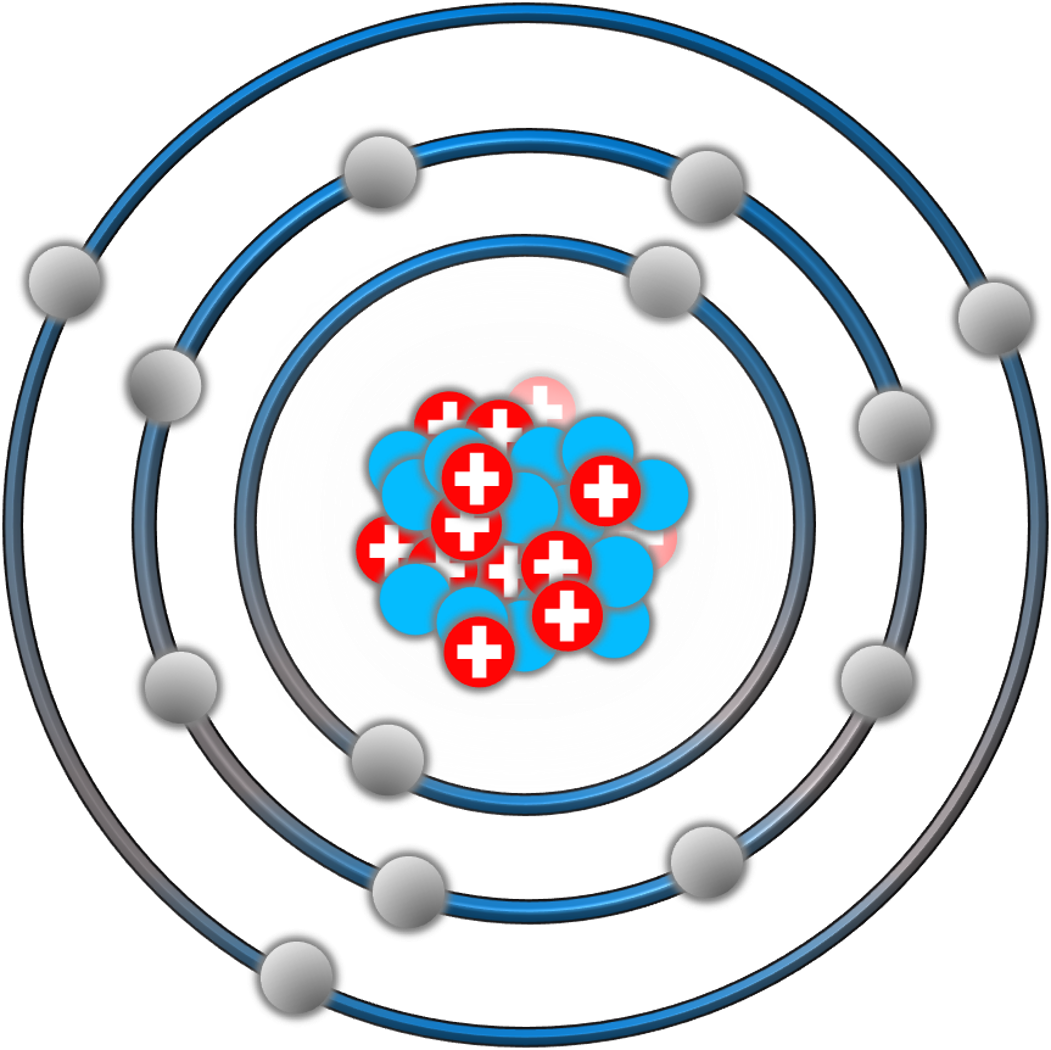
\includegraphics[width=3cm]{Images/anhminhoa/mohinhntbor.png}
		\captionof{figure}{Mô hình nguyên tử Rutherford - Bohr}
		\label{fig:mhntbo}
		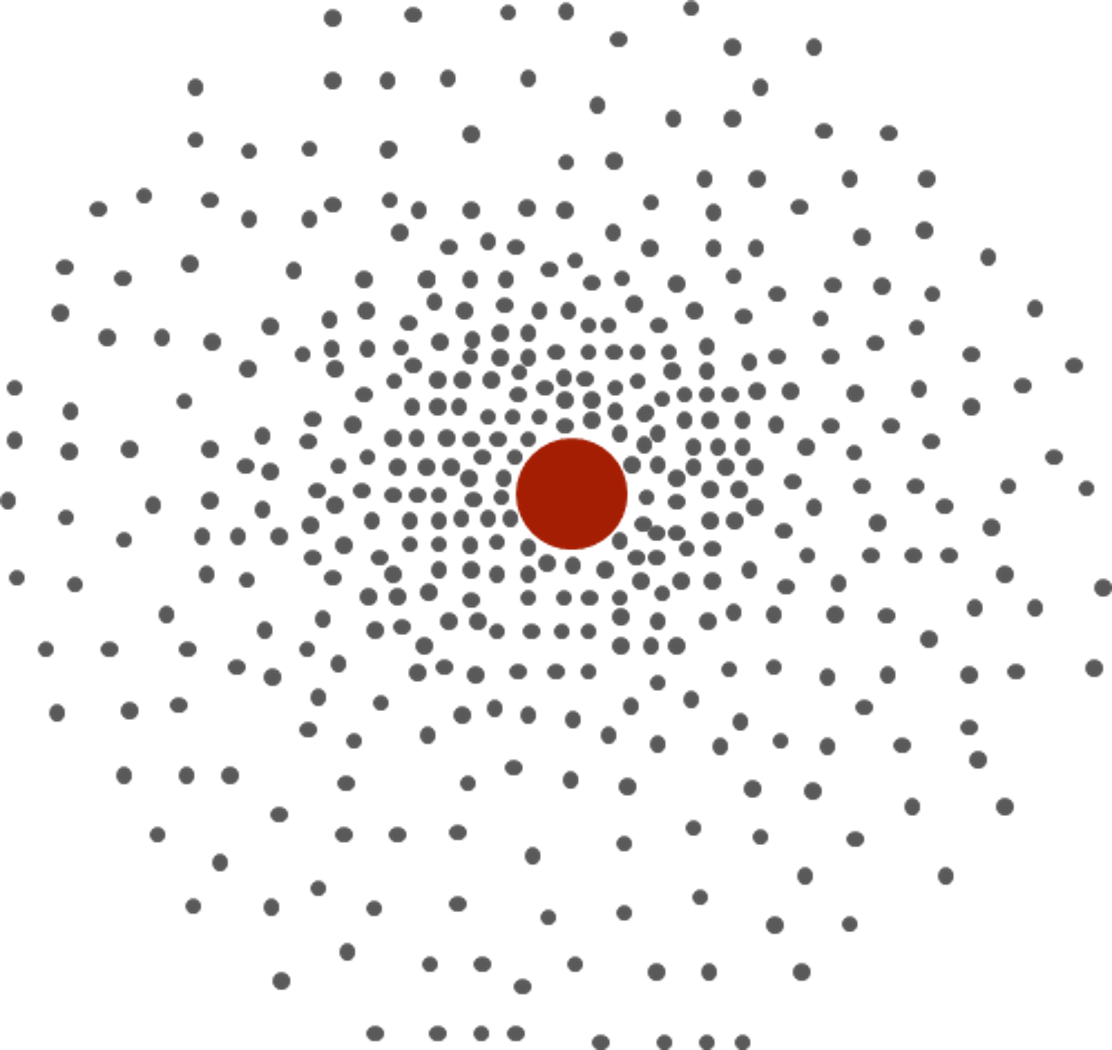
\includegraphics[width=3cm]{Images/anhminhoa/Mohinhnguyentuhiendai.png}
		\captionof{figure}{Mô hình nguyên tử hiện đại}
		\label{fig:mhnthd}
		\end{center}
\huongdan{
\begin{tabular}{|C{.25\textwidth}|L{0.65\textwidth}|}
\hline
\rowcolor{\mycolor!50!white} \multicolumn{1}{|c|}{ \sffamily\textbf{Mô hình} } & \multicolumn{1}{c|}{ \sffamily\textbf{Nội dung} } \\
\hline 
	Rutherford-Bohr &\makecell[l]{- Chưa có hạt neutron \\- Các electron quay xung quanh hạt nhân theo từng quỹ đạo\\ tròn ổn định, trong đó mỗi quỹ đạo có một mức năng lượng\\ xác định.}\\
\hline	
\makecell[c]{Hiện đại\\(Đám mây electron)} & \makecell[l]{- Đã tìm ra hạt neutron \\- Các electron chuyển độngh rất nhanh xung quanh hạt nhân\\ không theo một quỹ đạo xác định và tạo thành một đám mây\\ mang điện tích âm.}\\
\hline
\end{tabular}
}
\end{hoivadap}

\begin{emcobiet}
	Mô hình của Rutherford được gọi là mô hình mẫu hành tinh nguyên tử.
\end{emcobiet}
\subsubsection{Tìm hiểu về orbital nguyên tử}

\begin{dngsnd}
	\begin{itemize}
		\item \indam{Orbital nguyên tử} (Atomic Orbital, viết tắt $\mathrm{AO}$ ) là khu vực không gian xung quanh hạt nhân nguyên tử mà tại đó xác suất tìm thấy electron là lớn nhất (khoảng $90 \%$ ).
		\item Dựa trên sự khác nhau  về hình dạng và sự định hướng trong không gian của các orbital, người ta phân thành orbital s, orbital p, orbital d,orbital f
	\end{itemize}
\end{dngsnd}
Dưới đây là hình ảnh một số AO-s và AO-d (xem hình \ref{fig:hinhdangAO})\\
\begin{tikzpicture}
	% Định dạng cho cột của bảng
	\tikzset{%
		mynode/.style={%
		    ultra thick,
			minimum height=0.65cm,
			align=center,
			font=\sffamily
		},
		mymatrix/.style={%
			matrix of nodes,
			nodes={mynode},
			row 1/.style={%
				nodes={%
					fill=\mycolor!40!white,
					text centered,
					font=\bfseries\sffamily
				}
			},
			column 1/.style={%
				nodes={minimum width=0.25\textwidth}
			},
			column 2/.style={%
				nodes={minimum width=0.25\textwidth}
			},
			column 3/.style={%
				nodes={minimum width=0.25\textwidth}
			},
			column 4/.style={%
				nodes={minimum width=0.25\textwidth}
			}
		}
	}
	\matrix(Bang)[mymatrix]{%
	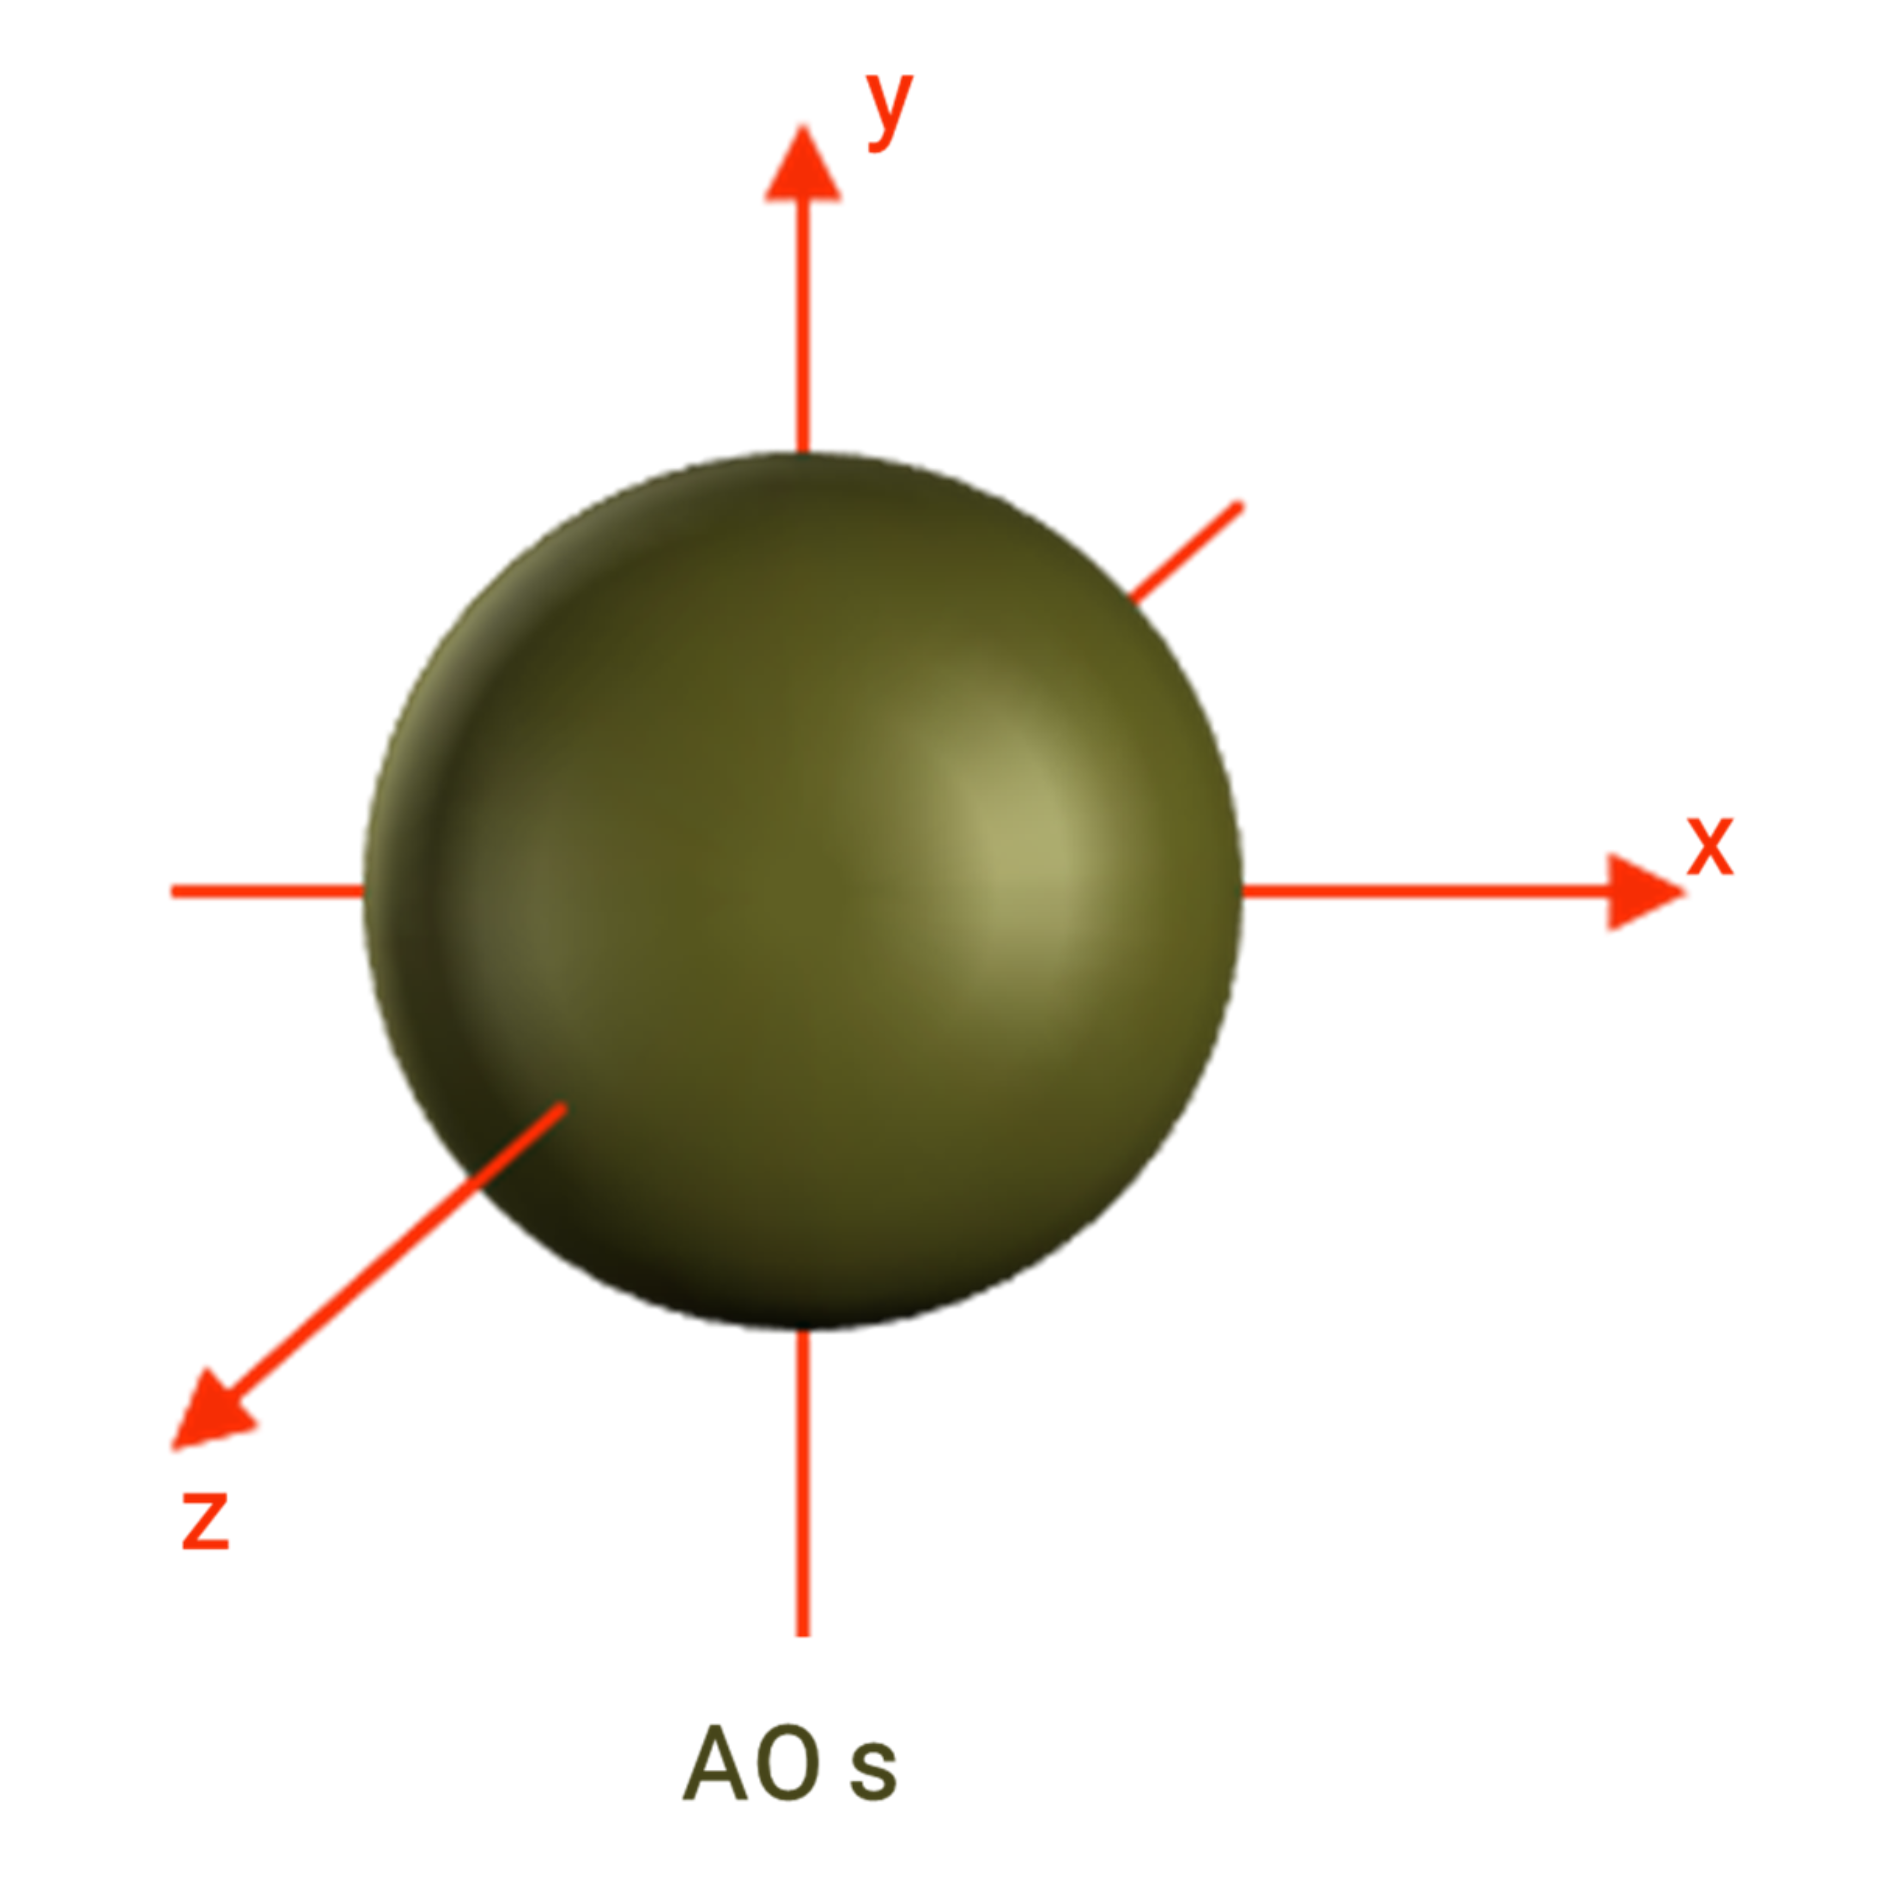
\includegraphics[width=3cm]{Images/anhminhoa/S.png}  & 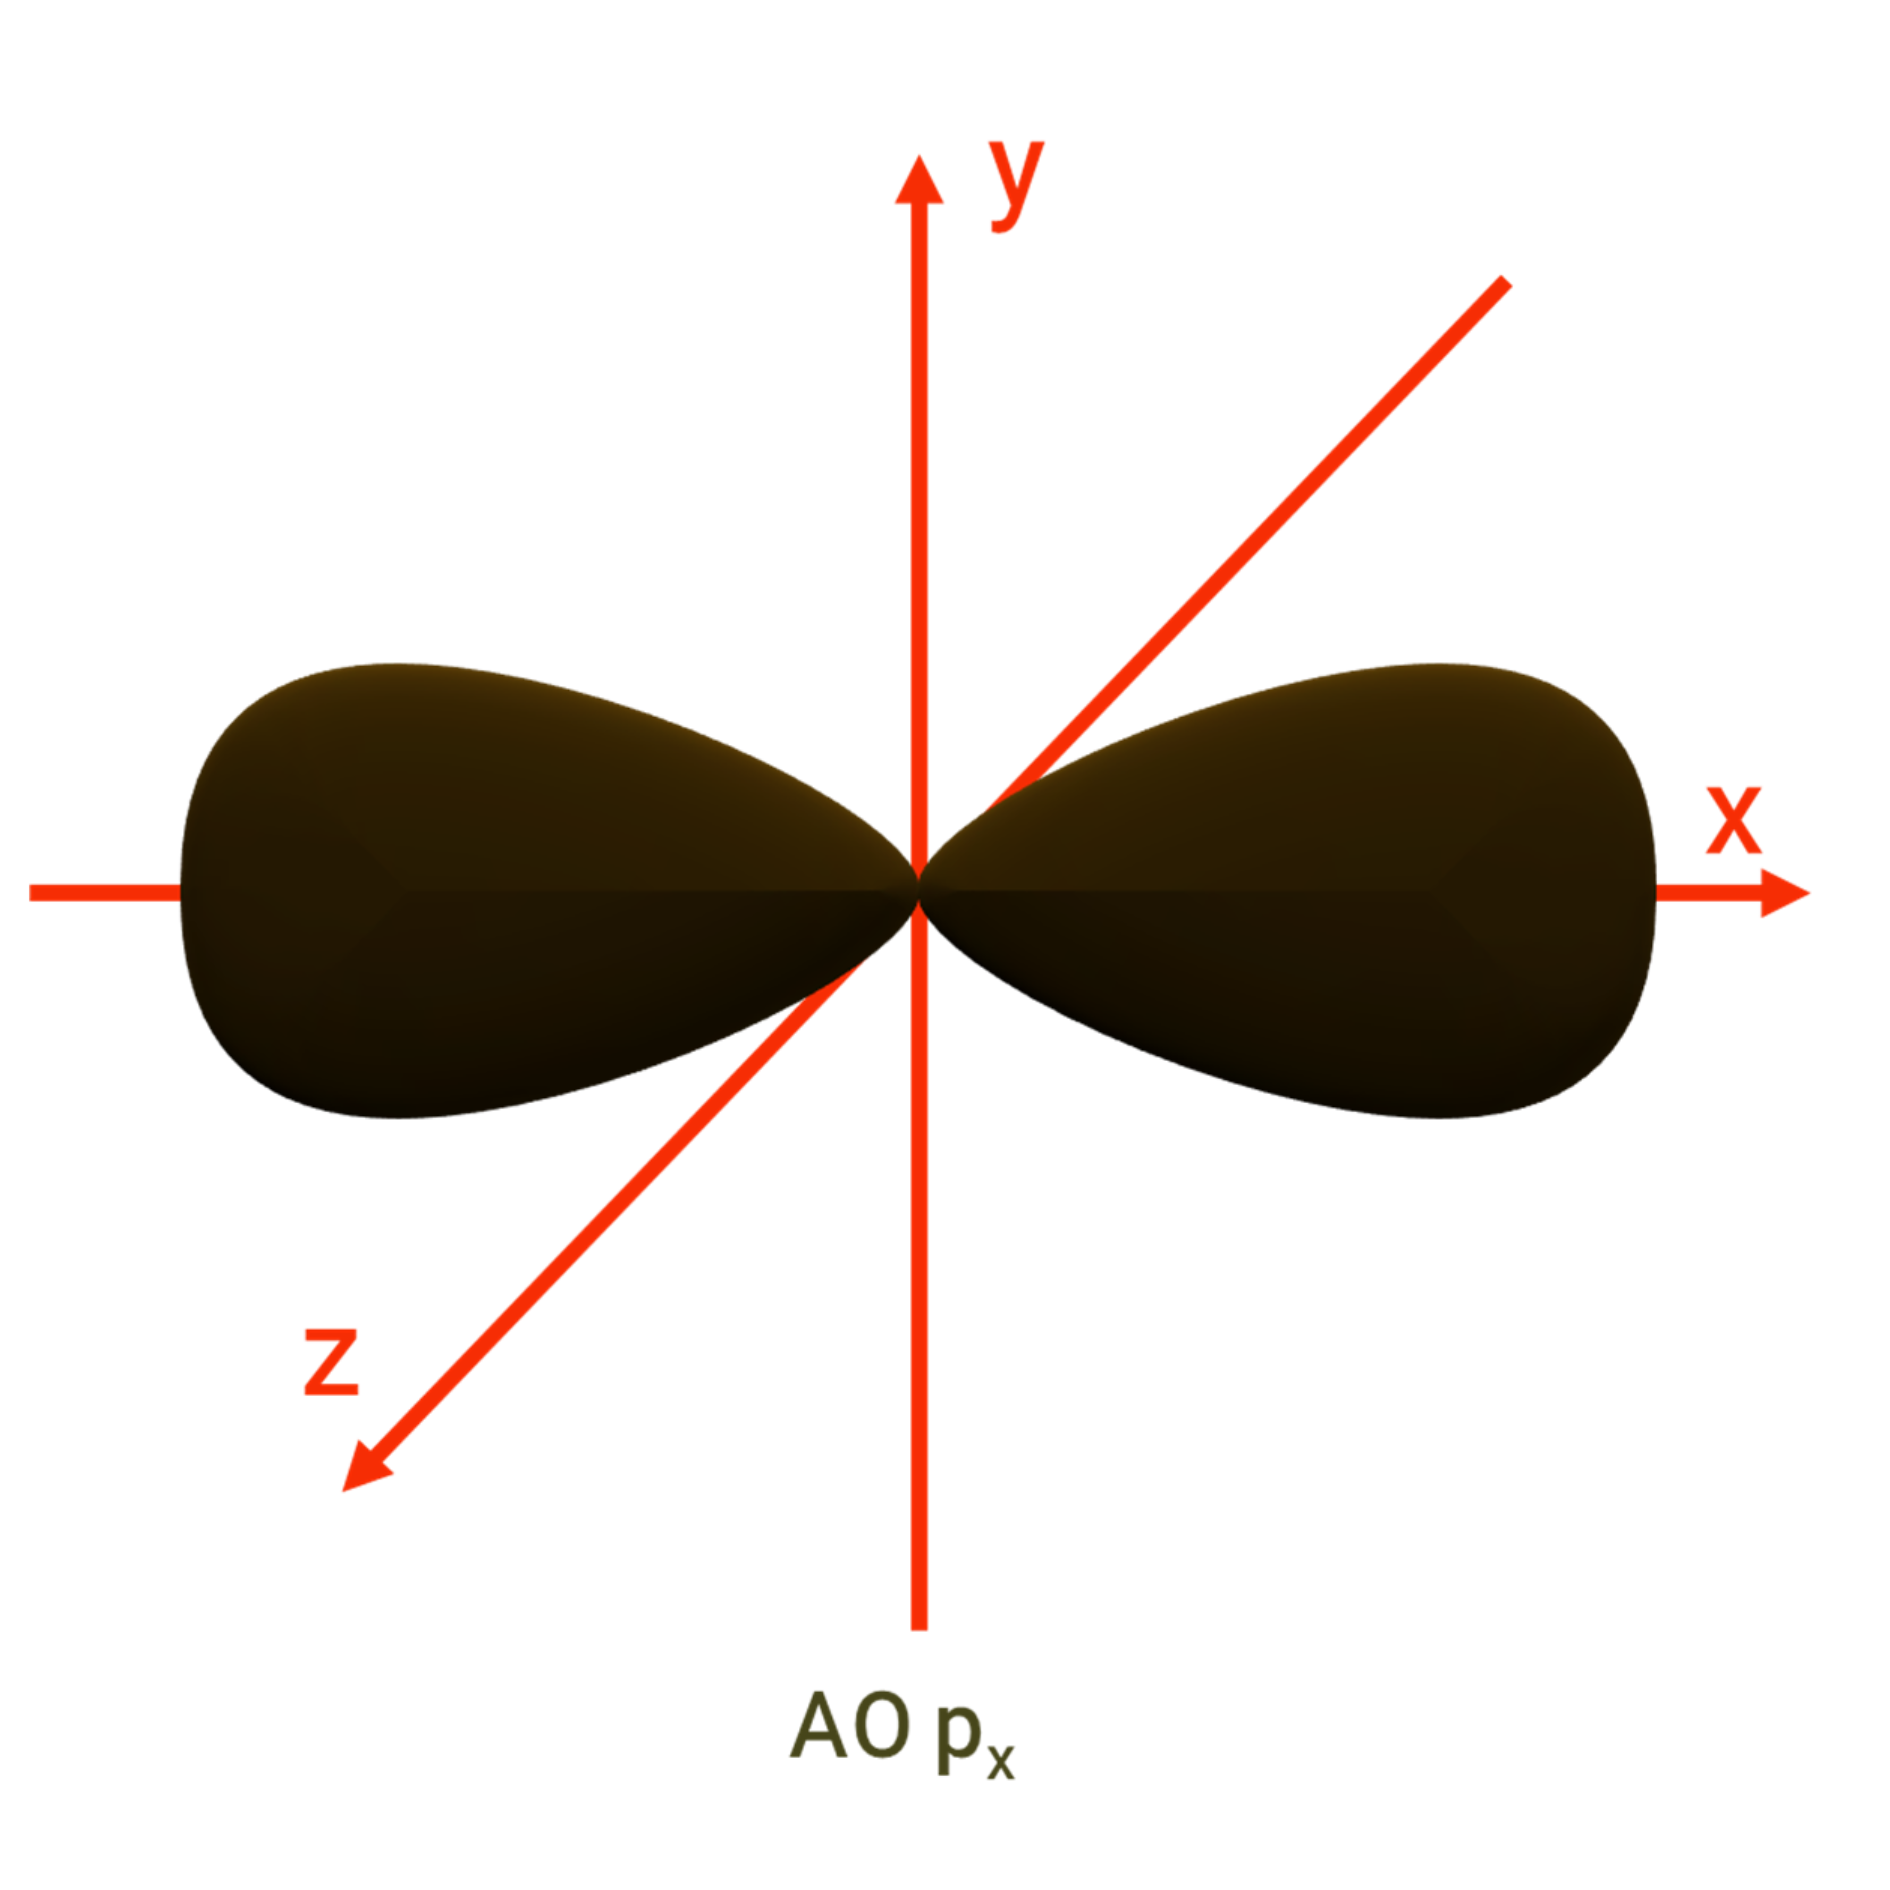
\includegraphics[width=3cm]{Images/anhminhoa/Px.png} & 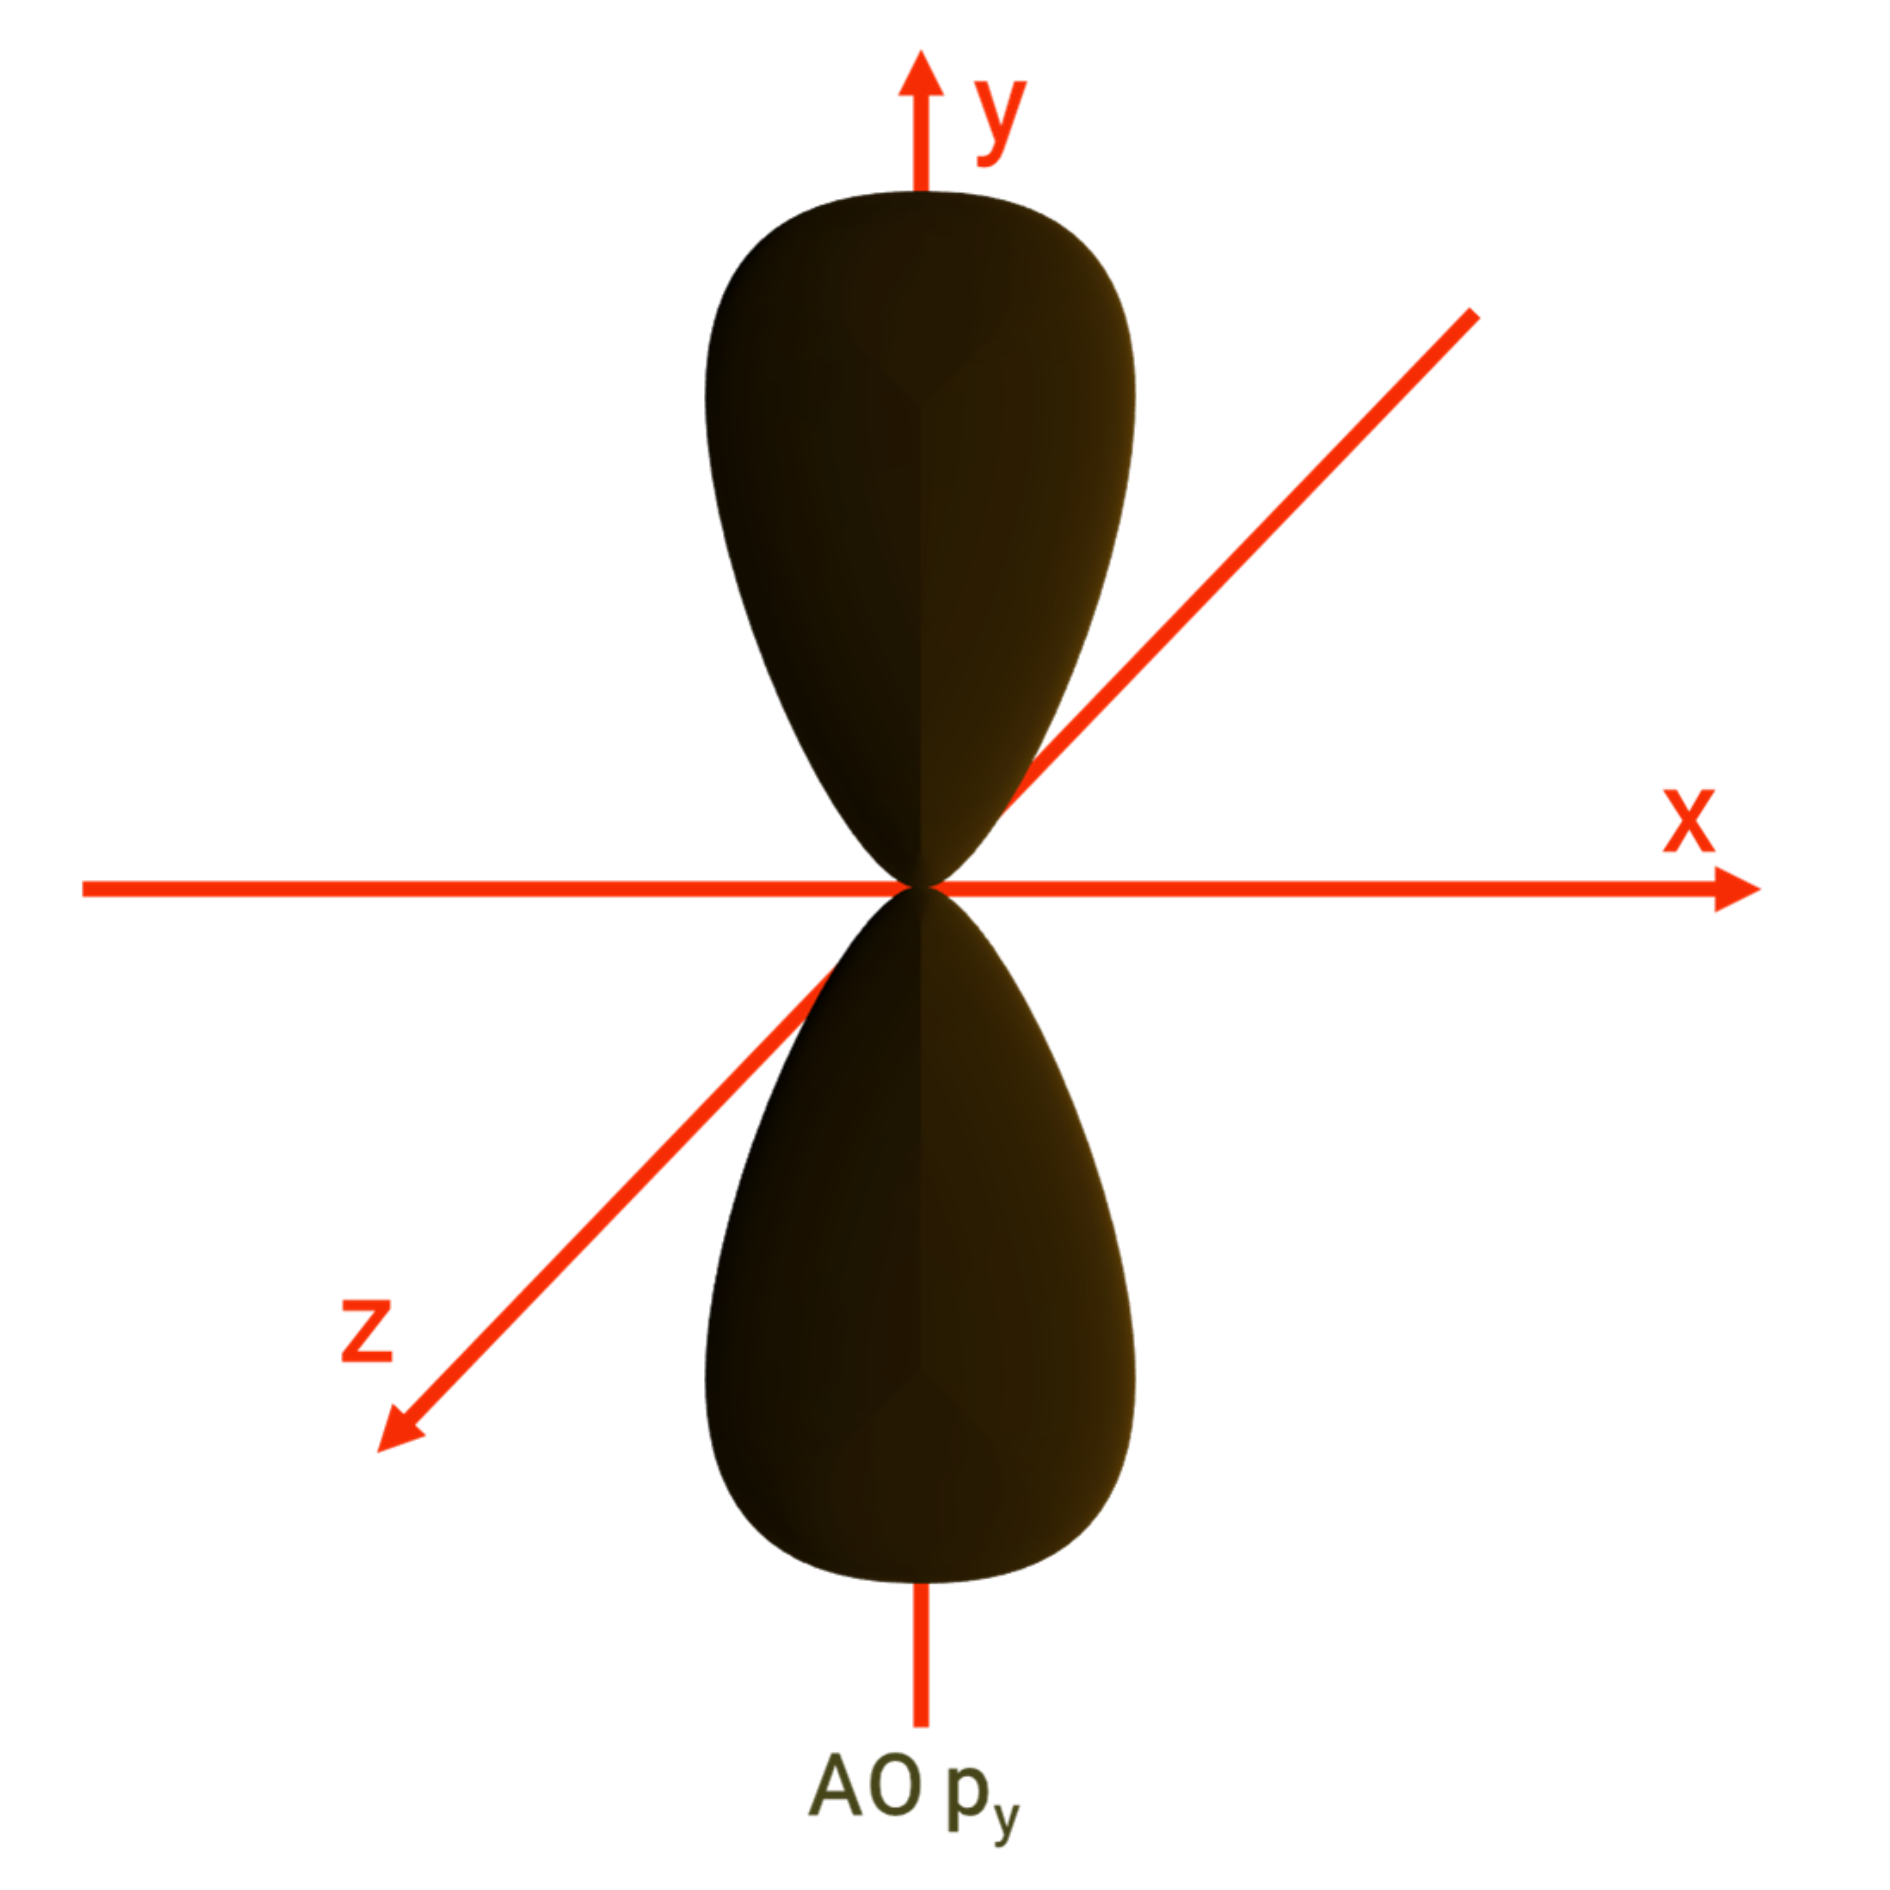
\includegraphics[width=3cm]{Images/anhminhoa/Py.png} &
	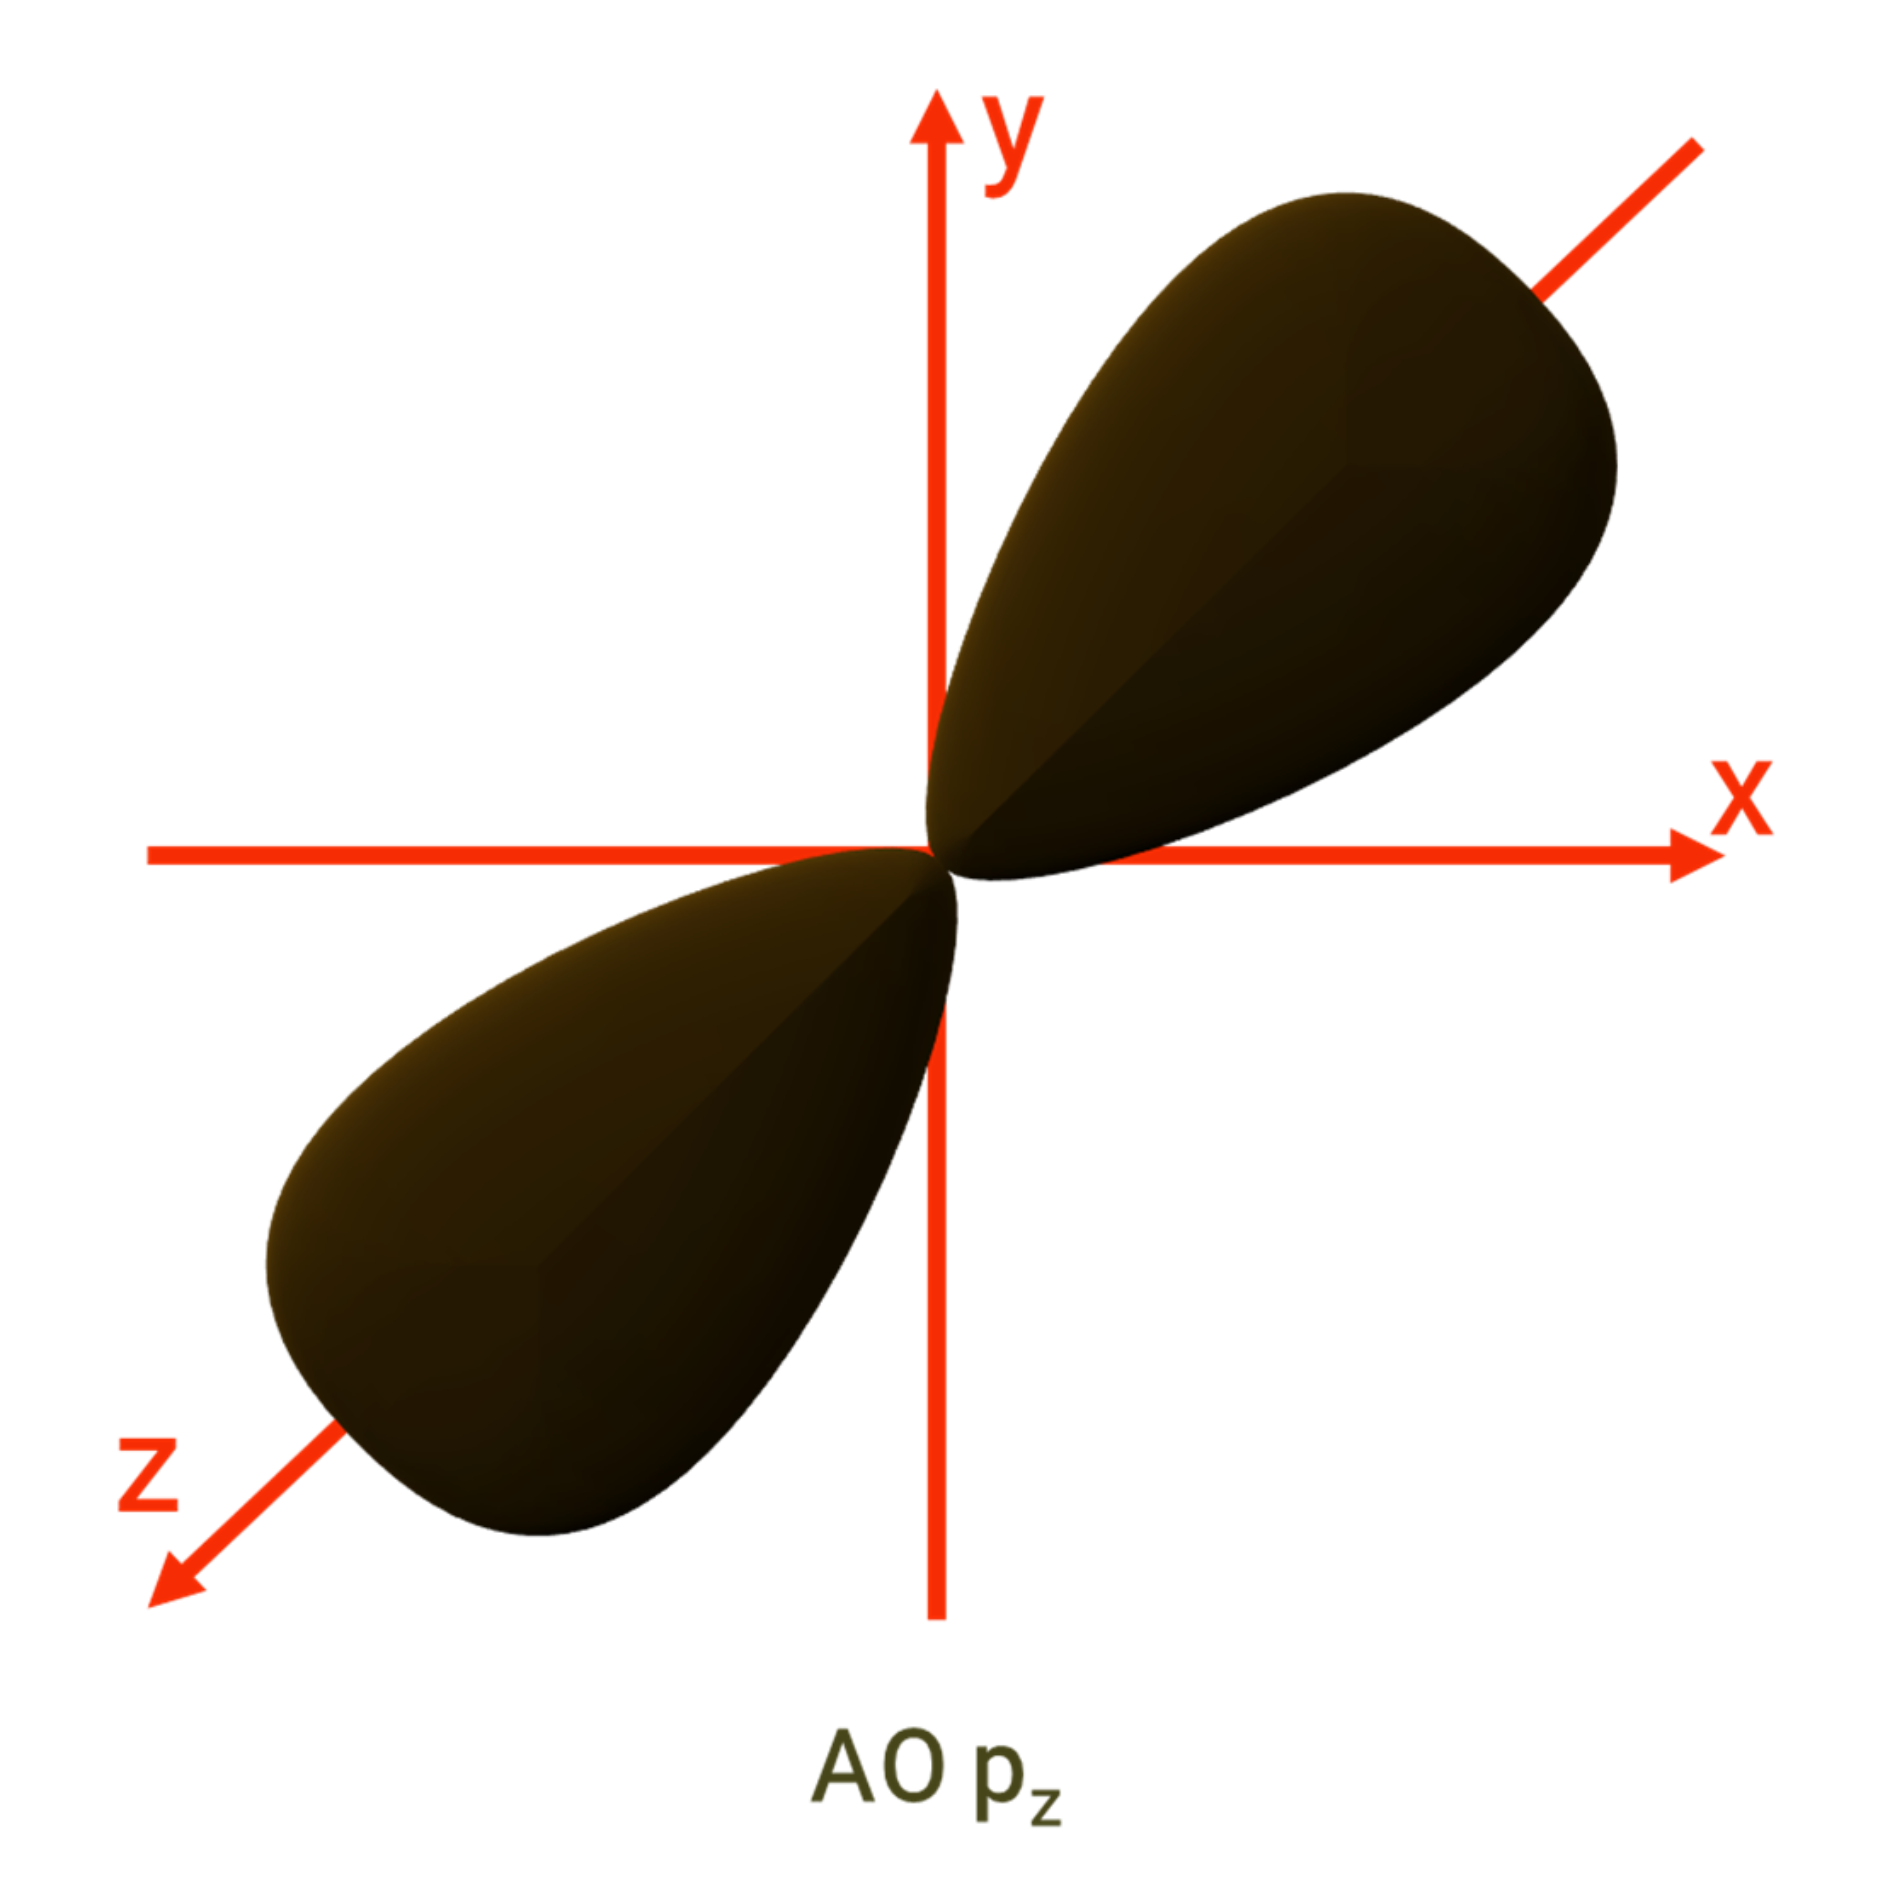
\includegraphics[width=3cm]{Images/anhminhoa/Pz.png}\\ 
	};
\end{tikzpicture}
\captionof{figure}{Hình dạng của các AO-s và AO-d}
\label{fig:hinhdangAO}
\subsection{Lớp và phân lớp electon}
\subsubsection{Lớp electron}

\begin{hoplythuyet}
	\begin{itemize}
	\item Trong nguyên tử, các electron được sắp xếp thành từng lớp ( kí hiệu lần lượt là:K,L,M,N,O,P,Q,...) và phân lớp theo mức năng lượng từ thấp đến cao.
	\item Các electron trên cùng  một lớp có mức năng lượng gần bằng nhau.
	\item Lớp electron gần hạt nhân nhất có năng lượng thấp nhất. càng xa hạt nhân năng lượng càng cao.
\end{itemize}
\end{hoplythuyet}
\begin{center}
	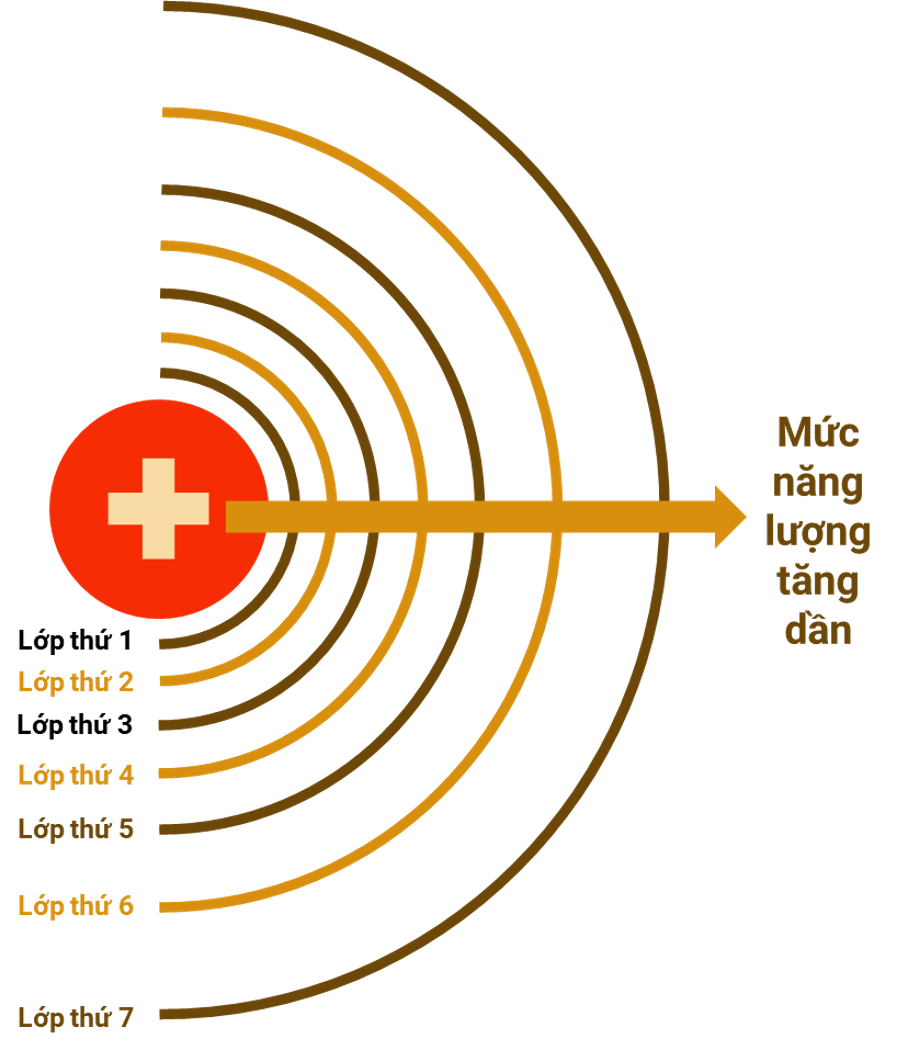
\includegraphics[height=6cm]{Images/anhminhoa/Lopelectron.png}
\end{center}
\subsubsection{Phân lớp electron}
\begin{hoplythuyet}
	\begin{itemize}
		\item Mỗi lớp electron chia thành các phân lớp ( Kí hiệu là: s, p, d, f)
		\item Các electron ở phân lớp s, p, d, f gọi là electron s, p, d, f.
		\item Các electron trên cùng một phân lớp thì có mức năng lượng bằng nhau
		\item Số phân lớp trong mỗi lớp bằng số thứ tự  của lớp đó.
	\end{itemize}
\end{hoplythuyet}

\begin{center}
%%=========Hình 4=========%%
\begin{tikzpicture}[declare function={r=3.0;}]
	\path [fill=cyan](0,0)-- (90:{r+5.6}) arc (90:0:{r+5.6}) -- cycle;
	\path [fill=violet](0,0)-- (90:{r+5.3}) arc (90:0:{r+5.3}) -- cycle;
	\path [fill=\mycolor](0,0)-- (90:{r+5}) arc (90:0:{r+5}) -- cycle;
	\path [fill=\mauphu](0,0) -- (90:{r+4.7}) arc (90:0:{r+4.7}) -- cycle;
	\path [fill=white](0,0)-- (90:{r+4.4}) arc (90:0:{r+4.4}) -- cycle;
	\path [fill=violet](0,0)-- (90:{r+3.6}) arc (90:0:{r+3.6}) -- cycle;
	\path [fill=\mycolor](0,0)-- (90:{r+3.3}) arc (90:0:{r+3.3}) -- cycle;
	\path [fill=\mauphu](0,0) -- (90:{r+3}) arc (90:0:{r+3}) -- cycle;
	\path [fill=white](0,0)-- (90:{r+2.7}) arc (90:0:{r+2.7}) -- cycle;
	\path [fill=\mycolor](0,0)-- (90:{r+2}) arc (90:0:{r+2}) -- cycle;
	\path [fill=\mauphu](0,0)-- (90:{r+1.7}) arc (90:0:{r+1.7}) -- cycle;
	\path [fill=white](0,0) -- (90:{r+1.4}) arc (90:0:{r+1.4}) -- cycle;
	\path [fill=\mauphu](0,0) -- (90:{r+.8}) arc (90:0:{r+.8}) -- cycle;
	\path [fill= white](0,0) -- (90:{r+.5}) arc (90:0:{r+.5}) -- cycle;
	\path [fill=\maunhan](0,0) -- (90:r) arc (90:0:r) -- cycle;
	\path ($(0,0)+(1.5,1.3)$) node[font=\color{white}\bfseries\sffamily,text width =2.5cm] {Hạt nhân nguyên tử};
%	\draw[%
%	decoration={%
%		text along path,
%        text={{\bfseries\sffamily H}{\bfseries\sffamily ử}{\bfseries\sffamily t} {\bfseries\sffamily n}{\bfseries\sffamily h}{\bfseries\sffamily â}{\bfseries\sffamily n} {\bfseries\sffamily n}{\bfseries\sffamily g}{\bfseries\sffamily u}{\bfseries\sffamily y}{\bfseries\sffamily ê}{\bfseries\sffamily n} {\bfseries\sffamily t}{\bfseries\sffamily ử}},
%		text align={center},
%		text color = white
%		},
%		decorate,
%		]
%		(90:{r-.4}) arc(90:0:{r-.4});
	\path 
	(0:{r+0.65}) node[font=\tiny\sffamily,below]{1s}
	(90:{r+0.65}) node[font=\tiny\sffamily,left,anchor=east]{Lớp thứ 1}
	(0:{r+1.55}) node[font=\tiny\sffamily,below]{2s}
	(90:{r+1.7}) node[font=\tiny\sffamily,left,anchor=east]{Lớp thứ 2}
	(0:{r+1.85}) node[font=\tiny\sffamily,below]{2p}
	(0:{r+2.85}) node[font=\tiny\sffamily,below]{3s}
	(0:{r+3.15}) node[font=\tiny\sffamily,below]{3p}
	(90:{r+3.15}) node[font=\tiny\sffamily,left,anchor=east]{Lớp thứ 3}
	(0:{r+3.45}) node[font=\tiny\sffamily,below]{3d}
	(0:{r+3.45}) node[font=\tiny\sffamily,below]{3d}
	(0:{r+4.55}) node[font=\tiny\sffamily,below]{4s}
	(0:{r+4.85}) node[font=\tiny\sffamily,below]{4p}
	(90:{r+5.0}) node[font=\tiny\sffamily,left,anchor=east]{Lớp thứ 4}
	(0:{r+5.15}) node[font=\tiny\sffamily,below]{4d}
	(0:{r+5.45}) node[font=\tiny\sffamily,below]{4f}
	;
\end{tikzpicture}
%%========= Hết hình4=========%
\captionof{figure}{Kí hiệu một số lớp và phân lớp trong nguyên tử}
\end{center}

\begin{center}
\begin{tikzpicture}[font=\normalsize]
	
\tikzset{%
%%Lưu tùy chọn vẽ đường tròn với tên ntdcircle	
ntdcircle/.style={%
	circle,
	fill=\maudam, % Màu và kiểu viền cho hình tròn
	inner sep=0pt,
	minimum size=.3cm % Kích thước hình tròn
},
mycircle/.pic={%
	\node[ntdcircle] at (0,0) {};
},
	%%% Đinh dạng trong 1 ô
	ntdnode/.style={%
		thick,
		anchor=center,
		align=center,
		minimum height = .4cm,
		minimum width = 2cm,
		font=\sffamily,
	},
	%%% Định dạng toàn cục
	ntdmatrix/.style={%
		matrix of nodes,
		inner sep =5pt,
		nodes in empty cells,
		fill =\mycolor!15,
		row sep=-\pgflinewidth,
		column sep=-\pgflinewidth,
		nodes={ntdnode},
		row 1/.style={%
			nodes={%
				fill=\mauphu!40!white,
				text centered,
				font=\bfseries\sffamily,
				draw=white,
%				ultra thick,
				inner sep =12pt
			}
		},
		row 2/.style={%
			nodes={%
				align=center,
				font=\bfseries\sffamily,
				inner sep =5pt,
				fill=\mauphu!20!white
			}
		},
		row 3/.style={%
			nodes={%
				align=center,
				font=\bfseries\sffamily,
				inner sep =5pt,
				fill=\mauphu!20!white
			}
		},
		row 4/.style={%
			nodes={%
				align=center,
				font=\bfseries\sffamily,
				inner sep =5pt,
				fill=\mauphu!40!white
			}
		},
		row 5/.style={%
			nodes={%
				align=center,
				font=\bfseries\sffamily,
				inner sep =5pt,
				fill=\mauphu!40!white
			}
		},
		row 6/.style={%
			nodes={%
				align=center,
				font=\bfseries\sffamily,
				inner sep =5pt,
				fill=\mauphu!20!white
			}
		},
		row 7/.style={%
			nodes={%
				align=center,
				font=\bfseries\sffamily,
				inner sep =5pt,
				fill=\mauphu!20!white
			}
		},
		row 8/.style={%
			nodes={%
				align=center,
				font=\bfseries\sffamily,
				inner sep =5pt,
				fill=\mauphu!40!white
			}
		},
		row 9/.style={%
			nodes={%
				align=center,
				font=\bfseries\sffamily,
				inner sep =5pt,
				fill=\mauphu!40!white
			}
		},
		column 1/.style={%
			nodes={%
				align=center,
				font=\bfseries\sffamily,
				inner sep =5pt
			}
		},
		column 5/.style={%
			nodes={%
				minimum width = 3.5cm,
			}
		},
	}
}

\matrix (ple) [ntdmatrix]{%
	 &  &  &  & \\
	 &  &  &  & \\
	 &  &  &  & \\
	 &  &  &  & \\
	 &  &  &  & \\
	 &  &  &  & \\
	 &  &  &  & \\
	 &  &  &  & \\
	 &  &  &  & \\
};
\fill[%
draw=white,
fill=\mauphu!60!white,
inner sep =5pt
]
(ple-1-1.north west)rectangle (ple-1-1.south east)node[anchor=center,midway,font=\bfseries\sffamily]{Lớp};
\fill[%
draw=white,
fill=\mauphu!60!white,
inner sep =5pt
]
(ple-1-1.north east)rectangle (ple-1-5.south east)node[anchor=center,midway,font=\bfseries\sffamily]{Phân lớp và số Orbital trên phân lớp};

\foreach \j/\n in {3/1s,5/2s,7/3s,9/4s}{%
	\path ([yshift=10pt]ple-\j-2.center) node[font=\sffamily] {\n};
	\foreach \i in {0}{%
		\draw 
		($(ple-\j-2.center)+(\i,0)$) pic{mycircle}
		;
	}

}

\foreach \j/\n in {5/2p,7/3p,9/4p}{%
	\path ([yshift=10pt]ple-\j-3.center) node[font=\sffamily] {\n};
	\foreach \i in {-0.35,0,.35}{%
		\draw 
		($(ple-\j-3.center)+(\i,0)$) pic{mycircle}
		;
	}
	
}

\foreach \j/\n in {7/3d,9/4d}{%
	\path ([yshift=10pt]ple-\j-4.center) node[font=\sffamily] {\n};
	\foreach \i in {-0.7,-0.35,0,.35,0.7}{%
		\draw 
		($(ple-\j-4.center)+(\i,0)$) pic{mycircle}
		;
	}
	
} 

\foreach \j in {9}{%
	\path ([yshift=10pt]ple-\j-5.center) node[font=\sffamily] {4f};
	\foreach \i in {-1.05,-0.7,-0.35,0,.35,0.7,1.05}{%
		\draw 
		($(ple-\j-5.center)+(\i,0)$) pic{mycircle}
		;
	}
} 

\foreach \x/\y/\z/\t in {20/2/3/1,40/4/5/2,20/6/7/3,40/8/9/4}{%
\fill[draw=white,fill=\mauphu!\x!white] (ple-\y-1.north west) rectangle (ple-\z-1.south east) node [anchor=center,midway,font=\bfseries\sffamily]{n=\t};
}

\end{tikzpicture}
\end{center}
\subsubsection{Cấu hình electron}
\paragraph{Nguyên lý vững bền}
\begin{hoplythuyet}
\GSND[\bfseries][\faTrello][\maunhan]{Nguyên lý vững bền}\\
\lq\lq Ở trạng thái cơ bản,các electron trong nguyên tử chiếm lần lượt những Orbital có mức năng lượng từ thấp đến cao.\rq\rq
\end{hoplythuyet}
%%%%%%%%%==============Nguyên lý vững bền==================%%%%%%%%%%
%\begin{center}
%		\begin{tikzpicture}[font=\Large,declare function={d=1.5cm; r={sqrt(2)/8 *d};}]
%			\tikzset{%a
%			ntdnode/.style={%
%				minimum height=0.65cm,
%				align=center,
%				font=\sffamily\bfseries,
%				minimum width =d,
%				minimum height =d,
%%				draw=cyan,
%			},
%			ntdmatrix/.style={%
%				matrix of nodes,
%				inner sep=5pt,
%				nodes in empty cells,
%%				fill=\mycolor!75,
%				row sep=-\pgflinewidth,
%				column sep=-\pgflinewidth,
%				nodes={ntdnode},
%				rounded corners=4pt,
%			},
%			line/.style={%
%			\maunhan!50!red,
%			arrows = {-Stealth},
%			line width=3pt,
%			}
%		}
%
%		\matrix (NLVB) [ntdmatrix] {%
%			 &  &  &  \\
%			 &  &  &  \\
%			 &  &  &  \\
%			 &  &  &  \\
%			 &  &  &  \\
%			 &  &  &  \\
%			 &  &  &  \\
%			 &  &  &  \\
%	};
%	
%	\draw (NLVB-1-1.south west) arc(135:315:r)
%	--(NLVB-1-1.east) arc(135:-45:r)--(NLVB-2-1.north east)
%	--(NLVB-2-1.south west) arc(135:315:r)--(NLVB-1-2.east) arc(135:-45:r)--(NLVB-2-2.north east)
%	--(NLVB-3-1.south west) arc(135:315:r)--(NLVB-2-2.east) arc(135:-45:r)--(NLVB-3-2.north east)
%	--(NLVB-4-1.south west) arc(135:315:r)--(NLVB-2-3.east) arc(135:-45:r)--(NLVB-3-3.north east)
%	--(NLVB-5-1.south west) arc(135:315:r)--(NLVB-3-3.east) arc(135:-45:r)--(NLVB-4-3.north east) 
%	--(NLVB-6-1.south west) arc(135:315:r)--(NLVB-3-4.east) arc(135:-45:r)--(NLVB-4-4.north east)
%	--(NLVB-7-1.south west) arc(135:315:r)--(NLVB-4-4.east) arc(135:-45:r)--(NLVB-5-4.north east)
%	;
%	
%	\foreach \h/\t/\n in {1/1/1,2/1/2,2/2/3,3/2/4,3/3/5,4/3/6,4/4/7,5/4/8}{%
%	\draw[line] (NLVB-\h-\t.north east)--(NLVB-\n-1.south west);	
%	}
%
%	
%	\foreach \i in {1,2,...,8}{%
%		\foreach \j in {1}{%
%			\path(NLVB-\i-\j.center) node[font=\bfseries\Large\sffamily,anchor=center]{\ntdshape{\i \color{\mycolor}{s}}}	;
%		}
%	}
%	\foreach \i in {2,3,...,7}{%
%		\foreach \j in {2}{%
%			\path(NLVB-\i-\j.center) node[font=\bfseries\Large\sffamily,anchor=center]{\ntdshape{\i \color{\maudam}{p}}}	;
%		}
%	}
%	\foreach \i in {3,4,...,6}{%
%		\foreach \j in {3}{%
%			\path(NLVB-\i-\j.center) node[font=\bfseries\Large\sffamily,anchor=center]{\ntdshape{\i \color{\maunhan}{d}}}	;
%		}
%	}
%	\foreach \i in {4,5}{%
%		\foreach \j in {4}{%
%			\path(NLVB-\i-\j.center) node[font=\bfseries\Large\sffamily,anchor=center]{\ntdshape{\i \color{\mauphu}{f}}}	;
%		}
%	}
%		\end{tikzpicture}
%	\captionof{figure}{Quy tắc Klechkowski }
%	\label{fig:Klechkowski}
%\end{center}

\begin{emcobiet}
		Các electron sắp sếp theo thứ tự mức năng lượng từ thấp đến cao được mô phỏng theo \indam{Quy tắc Klechkowski} (Xem hình \ref{fig:Klechkowski})\\
		Theo quy tắc này ta có trật tự mức năng lượng electron như sau:\\
		\begin{center}
		\boxct[\maunhan][3pt][\bfseries\sffamily][arc is angular]{1s,2s,2p,3p,4s,3d,4p,5s,4d,5p,6s,$\ldots$}
		\end{center}
		\begin{center}
			\begin{tikzpicture}[font=\Large,declare function={d=1.5cm; r={sqrt(2)/8 *d};}]
				\tikzset{%a
					ntdnode/.style={%
						minimum height=0.65cm,
						align=center,
						font=\sffamily\bfseries,
						minimum width =d,
						minimum height =d,
						%				draw=cyan,
					},
					ntdmatrix/.style={%
						matrix of nodes,
						inner sep=5pt,
						nodes in empty cells,
%						fill=\mycolor,
						row sep=-\pgflinewidth,
						column sep=-\pgflinewidth,
						nodes={ntdnode},
						rounded corners=4pt,
					},
					line/.style={%
						\maunhan!50!red,
						arrows = {-Stealth},
						line width=3pt,
					}
				}
				
				\matrix (NLVB) [ntdmatrix] {%
					&  &  &  \\
					&  &  &  \\
					&  &  &  \\
					&  &  &  \\
					&  &  &  \\
					&  &  &  \\
					&  &  &  \\
					&  &  &  \\
				};
				
				\draw (NLVB-1-1.south west) arc(135:315:r)
				--(NLVB-1-1.east) arc(135:-45:r)--(NLVB-2-1.north east)
				--(NLVB-2-1.south west) arc(135:315:r)--(NLVB-1-2.east) arc(135:-45:r)--(NLVB-2-2.north east)
				--(NLVB-3-1.south west) arc(135:315:r)--(NLVB-2-2.east) arc(135:-45:r)--(NLVB-3-2.north east)
				--(NLVB-4-1.south west) arc(135:315:r)--(NLVB-2-3.east) arc(135:-45:r)--(NLVB-3-3.north east)
				--(NLVB-5-1.south west) arc(135:315:r)--(NLVB-3-3.east) arc(135:-45:r)--(NLVB-4-3.north east) 
				--(NLVB-6-1.south west) arc(135:315:r)--(NLVB-3-4.east) arc(135:-45:r)--(NLVB-4-4.north east)
				--(NLVB-7-1.south west) arc(135:315:r)--(NLVB-4-4.east) arc(135:-45:r)--(NLVB-5-4.north east)
				;
				
				\foreach \h/\t/\n in {1/1/1,2/1/2,2/2/3,3/2/4,3/3/5,4/3/6,4/4/7,5/4/8}{%
					\draw[line] (NLVB-\h-\t.north east)--(NLVB-\n-1.south west);	
				}
				
				
				\foreach \i in {1,2,...,8}{%
					\foreach \j in {1}{%
						\path(NLVB-\i-\j.center) node[font=\bfseries\Large\sffamily,anchor=center]{\ntdshape{\i \color{\mycolor}{s}}}	;
					}
				}
				\foreach \i in {2,3,...,7}{%
					\foreach \j in {2}{%
						\path(NLVB-\i-\j.center) node[font=\bfseries\Large\sffamily,anchor=center]{\ntdshape{\i \color{\maudam}{p}}}	;
					}
				}
				\foreach \i in {3,4,...,6}{%
					\foreach \j in {3}{%
						\path(NLVB-\i-\j.center) node[font=\bfseries\Large\sffamily,anchor=center]{\ntdshape{\i \color{\maunhan}{d}}}	;
					}
				}
				\foreach \i in {4,5}{%
					\foreach \j in {4}{%
						\path(NLVB-\i-\j.center) node[font=\bfseries\Large\sffamily,anchor=center]{\ntdshape{\i \color{\mauphu}{f}}}	;
					}
				}
			\end{tikzpicture}
			\captionof{figure}{Quy tắc Klechkowski }
			\label{fig:Klechkowski}
		\end{center}
\end{emcobiet}

\paragraph{Nguyên lý pauli}

\begin{hoplythuyet}
	\indam{Nguyên lí Pauli:} Mỗi orbital chỉ chứa tối đa 2 electron và có chiều tự quay ngược nhau.
\end{hoplythuyet}

\begin{tikzpicture}
	\path (0,0) node[anchor=center](eghepdoi) {\Eghepdoi}
	      (eghepdoi.east) node [xshift=-5pt,anchor=west]{:\ \indam{Electron ghép đôi}}
	;
	
	\path (0,-1) node[anchor=center](edocthan) {\Edocthan}
	(edocthan.east) node [xshift=-5pt,anchor=west]{:\ \indam{Electron độc thân}}
	;
\end{tikzpicture}
\paragraph{Xác định số AO và số electron tối đa trong một phân lớp và trong mỗi lớp}

\begin{tikzpicture}[font=\normalsize,declare function={d=2.6cm;r=.9cm;}]
	\tikzset{%a
		ntdnode/.style={%
			align=center,
			font=\sffamily\bfseries,
			minimum width =d,
			minimum height =r,
			draw=white,
			anchor =center,
			fill=\mycolor!75,
		},
		ntdmatrix/.style={%
			matrix of nodes,
			inner sep=5pt,
			nodes in empty cells,
%			fill=\mycolor!15,
			row sep=-\pgflinewidth,
			column sep=-\pgflinewidth,
			nodes={ntdnode},
%			rounded corners=4pt,
		column 1/.style={%
			nodes={%
				align=center,
				font=\bfseries\sffamily,
				inner sep =5pt,
				minimum width =1.2cm
			}
		},
		row 1/.style={%
			nodes={%
				align=center,
				font=\color{white}\bfseries\sffamily,
				inner sep =5pt,
				minimum height =2cm,
				fill=\maudam!85
			}
		},		
		column 4/.style={%
			nodes={%
				minimum width =3.4cm
			}
		},
		column 5/.style={%
			nodes={%
				minimum width =3.8cm
			}
		},
		column 6/.style={%
			nodes={%
				minimum width =3.6cm
			}
		},	
	},
		line/.style={%
			\maunhan!50!red,
			arrows = {-Stealth},
			line width=3pt,
		}
	}
	\matrix (soelectron) [ntdmatrix] {%
	n	& Tên lớp & \makecell{Tên \\phân lớp} & \makecell{Số AO\\ trong mỗi\\ phân lớp} & \makecell{Số e \\tối đa trong\\ mỗi phân lớp} & \makecell[c]{Số e \\tối đa trong\\ một lớp} \\
		&  & s & 1 & 2 &  \\
		&  & s & 1 & 2 &  \\
		&  & p & 3 & 6 &  \\
		&  & s & 1 & 2 &  \\
		&  & p & 3 & 6 &  \\
		&  & d &  5& 10& \\
		&  & s & 1 & 2 &  \\
		&  & p & 3 & 6 &  \\
		&  & d & 5 & 10&  \\
		&  & f & 7 & 14&  \\
	n	&  & $n^2$ &   & &  \\
	};
\foreach \i/\j/\k in {2/2/1,3/4/2,5/7/3,8/11/4,12/12/n}{%
\path[draw=white,fill=\mycolor!75](soelectron-\i-1.north west) rectangle (soelectron-\j-1.south east)node[midway,anchor=center]{\indam{\k}};
}	

\foreach \i/\j/\k in {2/2/K,3/4/L,5/7/M,8/11/N}{%
	\path[draw=white,fill=\mycolor!75](soelectron-\i-2.north west) rectangle (soelectron-\j-2.south east)node[midway,anchor=center]{\indam[black]{\k}};
}

\foreach \i/\j/\k in {2/2/$2=2\cdot1^2$,3/4/$8=2\cdot2^2$,5/7/$18=2\cdot3^2$,8/11/$32=2\cdot4^2$,12/12/$2n^2$}{%
	\path[draw=white,fill=\mycolor!75](soelectron-\i-6.north west) rectangle (soelectron-\j-6.south east)node[midway,anchor=center]{\indam[black]{\k}};
}
\path[draw=white,fill=\mycolor!75](soelectron-12-2.north west) rectangle (soelectron-12-5.south east)node[midway,anchor=center]{\indam[black]{$n^2$}};	
\end{tikzpicture}
\paragraph{Quy tắc hund}
\begin{hoplythuyet}
	\lq \lq Trong cùng một phân lớp chưa bão hòa, các electron sẽ phân bố vào các AO sao cho số e độc thân là tối đa\rq \rq
\end{hoplythuyet}


\begin{hoivadap}
	Trong các trường hợp dưới đây trường hợp nào các electron điền e vào các orbital theo các nguyên lý và quy tắc đã học
\begin{myenum}
	\item
	\begin{adjustbox}{valign=m}
		\begin{tikzpicture}[declare function={x=.896cm;l=1.2;}]   
			\path(0:{0*x}) node [anchor=center](dxy) {\Eghepdoi}
			(0:{1*x}) node [anchor=center](dyz) {\Eghepdoi}
			(0:{2*x}) node [anchor=center](dzz) {\Eghepdoi}
			(0:{3*x}) node [anchor=center](pxxyy) {\Eghepdoi}
			(0:{4*x}) node [anchor=center](pxz) {\Edocthan};
			\path (0:{5*x}) node [anchor=center,transform canvas={shift={(10pt,-3pt)}}](ssss) {\Edocthan[\maunhan]};
			\path([xshift=15pt]ssss.south)node[anchor=north]{$4s^1$};
			\path([xshift=3.2pt]dzz.south)node[anchor=north]{$3d^{9}$};
		\end{tikzpicture}
	\end{adjustbox}
	\item
	\begin{adjustbox}{valign=m}
		\begin{tikzpicture}[declare function={x=.896cm;l=1.2;}]  
			\path(0:{0*x}) node [anchor=center](dxy) {\Eghepdoi}
			(0:{1*x}) node [anchor=center](dyz) {\Eghepdoi}
			(0:{2*x}) node [anchor=center](dzz) {\Edocthan}
			(0:{3*x}) node [anchor=center](pxxyy) {\Edocthan}
			(0:{4*x}) node [anchor=center](pxz) {\Edocthan};
			\path (0:{5*x}) node [anchor=center,transform canvas={shift={(10pt,-3pt)}}](ssss) {\Eghepdoi[\maunhan]};
			\path([xshift=15pt]ssss.south)node[anchor=north]{$4s^2$};
			\path([xshift=3.2pt]dzz.south)node[anchor=north]{$3d^{9}$};
		\end{tikzpicture}
	\end{adjustbox}
	\item
	\begin{adjustbox}{valign=m}
		\begin{tikzpicture}[declare function={x=.896cm;l=1.2;}]  
			\path(0:{0*x}) node [anchor=center](SSS) {\Eghepdoi}
			(0:{1*x}) node [anchor=center,transform canvas={shift={(10pt,3pt)}}](p) {\Eghepdoi}
			(0:{2*x}) node [anchor=center,transform canvas={shift={(10pt,3pt)}}](pp) {\Eghepdoi}
			(0:{3*x}) node [anchor=center,transform canvas={shift={(10pt,3pt)}}](ppp) {\AOtrong};
			\path([xshift=5pt]SSS.south)node[anchor=north]{$3s^2$};
			\path([xshift=14pt]pp.south)node[anchor=north]{$3p^{4}$};
		\end{tikzpicture}
	\end{adjustbox}
\end{myenum}
\end{hoivadap}

\begin{notegsnd}
%%%%=================== Phan lop d========================%%%%%%%%%%%%%
\begin{tikzpicture}[declare function={d=.6cm;r={d/2.4};}]
		\tikzset{
			eghepdoi/.pic={
				\draw[arrows={-Stealth}, line width=1pt, \maudam]
				(0,0)--(0,d);
				\draw[arrows={-Stealth}, line width=1pt, \maudam]
				(r,d)--(r,0);
			},
			edocthan/.pic={
				\draw[arrows={-Stealth}, line width=1pt, \maudam]
				(0,0)--(0,d);
			},
			echuaghepdoi/.pic={
				\draw[arrows={-Stealth}, line width=1pt, \maudam]
				(0,0)--(0,d);
				\path[arrows={-Stealth}, line width=1pt, \maudam]
				(r,d)--(r,0);
			}
		}
%%%%%%%%%%%%%%%%%%%%%%%Cấu hình 3d bão hòa%%%%%%%%%%%%%%%%%%%%%%%%%%%%%%
	\matrix (pld)[%
	matrix of nodes,
	nodes={%
		draw= \maudam,
		thick,
		minimum height =.8cm,
		minimum width = .8cm,
		anchor = center,
		align =center,
		inner sep =3pt,
	},
	nodes in empty cells,
	row sep=-\pgflinewidth,
	column sep=-\pgflinewidth,
	]{%
		& & & &\\
	};
%%%%%%%%%%%%%%%%%%%%%%%%%%%%%%%%%%%%%%%%%%%%%%%%%%%%%%%%%%%%%%%%%%%%%%%%%%%%%%%%	
	\begin{scope}[transform canvas={xshift=-3.7pt,yshift=-8.7pt}]
	\foreach \x in {1,2,3,4,5}{
		\draw(pld-1-\x.center) pic {eghepdoi};
	}
\end{scope}	

\path (pld.south) node[anchor=north,font=\small] {Cấu hình bão hòa (bền)};
	\end{tikzpicture}
%%%%%%%%%%%%%%%%%%%%%%%%Cấu hình 3d Bán bão hòa=======================%%%%%%%%%%%%%%%%%%%%%%%%	
	\begin{tikzpicture}[declare function={d=.60cm;r={d/2.4};}]
	\tikzset{
		eghepdoi/.pic={
			\draw[arrows={-Stealth}, line width=1pt, \maudam]
			(0,0)--(0,d);
			\draw[arrows={-Stealth}, line width=1pt, \maudam]
			(r,d)--(r,0);
		},
		edocthan/.pic={
			\draw[arrows={-Stealth}, line width=1pt, \maudam]
			(0,0)--(0,d);
		},
		echuaghepdoi/.pic={
			\draw[arrows={-Stealth}, line width=1pt, \maudam]
			(0,0)--(0,d);
			\path[arrows={-Stealth}, line width=1pt, \maudam]
			(r,d)--(r,0);
		}
	}
	%%%%%%%%%%%%%%%%%%%%%%%%%%%%%%%%%%%%%%%%%%%%%%%%%%%%%%%%%%%%%%%%%%%%%%%%%%%%%%%%
	\matrix (pld)[%
	matrix of nodes,
	nodes={%
		draw= \maudam,
		thick,
		minimum height =.8cm,
		minimum width = .8cm,
		anchor = center,
		align =center,
		inner sep =3pt,
	},
	nodes in empty cells,
	row sep=-\pgflinewidth,
	column sep=-\pgflinewidth,
	]{%
		& & & &\\
	};
	%%%%%%%%%%%%%%%%%%%%%%%%%%%%%%%%%%%%%%%%%%%%%%%%%%%%%%%%%%%%%%%%%%%%%%%%%%%%%%%%	
	\begin{scope}[transform canvas={xshift=-0.5pt,yshift=-8.7pt}]
		\foreach \x in {1,2,3,4,5}{
			\draw(pld-1-\x.center) pic {edocthan};
		}
	\end{scope}	
\path (pld.south) node[anchor=north,font=\small] {Cấu hình bán bão hòa (bền)};	
\end{tikzpicture}	
%%%%%%%%%%%%%%%%%%%%%%%%Cấu hình 3d chưa bão hòa=======================%%%%%%%%%%%%%%%%%%%%%%%%	
\begin{tikzpicture}[declare function={d=.60cm;r={d/2.4};}]
	\tikzset{
		eghepdoi/.pic={
			\draw[arrows={-Stealth}, line width=1pt, \maudam]
			(0,0)--(0,d);
			\draw[arrows={-Stealth}, line width=1pt, \maudam]
			(r,d)--(r,0);
		},
		edocthan/.pic={
			\draw[arrows={-Stealth}, line width=1pt, \maudam]
			(0,0)--(0,d);
		},
		echuaghepdoi/.pic={
			\draw[arrows={-Stealth}, line width=1pt, \maudam]
			(0,0)--(0,d);
			\path[arrows={-Stealth}, line width=1pt, \maudam]
			(r,d)--(r,0);
		}
	}
	%%%%%%%%%%%%%%%%%%%%%%%%%%%%%%%%%%%%%%%%%%%%%%%%%%%%%%%%%%%%%%%%%%%%%%%%%%%%%%%%
	\matrix (pld)[%
	matrix of nodes,
	nodes={%
		draw= \maudam,
		thick,
		minimum height =.8cm,
		minimum width = .8cm,
		anchor = center,
		align =center,
		inner sep =3pt,
	},
	nodes in empty cells,
	row sep=-\pgflinewidth,
	column sep=-\pgflinewidth,
	]{%
		& & & &\\
	};
	%%%%%%%%%%%%%%%%%%%%%%%%%%%%%%%%%%%%%%%%%%%%%%%%%%%%%%%%%%%%%%%%%%%%%%%%%%%%%%%%	
	\begin{scope}[transform canvas={xshift=-3pt,yshift=-8.7pt}]
		\foreach \x in {1,2,3}{
			\draw(pld-1-\x.center) pic {eghepdoi};
		}
	\end{scope}	
	\begin{scope}[transform canvas={xshift=-0.5pt,yshift=-8.7pt}]
			\foreach \x in {4,5}{
			\draw(pld-1-\x.center) pic {edocthan};
		}
	\end{scope}
	\path (pld.south) node[anchor=north,font=\small] {Cấu hình chưa bão hòa (kém bền)};	
\end{tikzpicture}
\GSND[][\faBell][\maunhan]{Một số cấu hình đặc biệt: ${}_{29}Cu$	và ${}_{24}Cr$}
\begin{itemize}
\item Cấu hình của ${}_{29}Cu$ theo quy luật sẽ là $[Ar]3d^94s^2$ [\footnote{Cách viết cấu hình thu gọn}].Tuy nhiên một electron từ phân lớp 4s tham gia ghép đôi với 1 e độc thân ở 3d để đạt trạng thái bão hào ở phân lớp 3d $[Ar]3d^{10}4s^1$ bền vững hơn.\\
\begin{tikzpicture}	[declare function={x=.896cm;l=1.2;}]	
	\path(0:{0*x}) node [anchor=center](dxy) {\Eghepdoi}
	(0:{1*x}) node [anchor=center](dyz) {\Eghepdoi}
	(0:{2*x}) node [anchor=center](dzz) {\Eghepdoi}
	(0:{3*x}) node [anchor=center](pxxyy) {\Eghepdoi}
	(0:{4*x}) node [anchor=center](pxz) {\Ecbghepdoi[\maunhan]}
	;
	\path([xshift=3.2pt]dzz.south)node[anchor=north]{$3d^9$};
	\begin{scope}[transform canvas={shift={(10pt,-3pt)}}]
		\path (0:{5*x}) node [anchor=center](ssss) {\Eghepdoi[\maunhan]};
		\path([xshift=3.2pt]ssss.south)node[anchor=north]{$4s^2$};
	\end{scope}
	\path(0:{9*x}) node [anchor=center](dxy1) {\Eghepdoi}
	(0:{10*x}) node [anchor=center](dyz1) {\Eghepdoi}
	(0:{11*x}) node [anchor=center](dzz1) {\Eghepdoi}
	(0:{12*x}) node [anchor=center](pxxyy1) {\Eghepdoi}
	(0:{13*x}) node [anchor=center](pxz1) {\Eghepdoi[\maunhan]}
	;
	\path([xshift=3.2pt]dzz1.south)node[anchor=north]{$3d^{10}$};
	\begin{scope}[transform canvas={shift={(10pt,-3pt)}}]
		\path (0:{14*x}) node [anchor=center](ssss1) {\Ecbghepdoi[\maunhan]};
		\path([xshift=3.2pt]ssss1.south)node[anchor=north]{$4s^1$};
	\end{scope}
%	\draw[->,arrows={-Stealth}, line width=1pt]([xshift=16pt]ssss.east)--(dxy1.west);
	\draw[->,arrows={-Stealth}, line width=1pt]([xshift=16pt]ssss.east)--(dxy1.west);
	\draw[\maunhan,->,arrows={-Stealth}, line width=1pt]([xshift=.6cm,yshift=-2pt]ssss.north) .. controls+(90:l) and +(90:l) .. ([xshift=10pt]pxz.north);
\end{tikzpicture}\\
\item Cấu hình của ${}_{24}Cr$:Tương tự như vậy cấu hình đúng của Cr là $[Ar]3d^{5}4s^{1}$ (cấu hình bán bão hòa) thay vì $ [Ar]3d^{4}4s^{2}$\\
\begin{tikzpicture}	[declare function={x=.896cm;l=1.2;}]	
	\path(0:{0*x}) node [anchor=center](dxy) {\Edocthan}
	(0:{1*x}) node [anchor=center](dyz) {\Edocthan}
	(0:{2*x}) node [anchor=center](dzz) {\Edocthan}
	(0:{3*x}) node [anchor=center](pxxyy) {\Edocthan}
	(0:{4*x}) node [anchor=center](pxz) {\AOtrong[\maunhan][.633cm]}
	;
	\path([xshift=3.2pt]dzz.south)node[anchor=north]{$3d^4$};
	\begin{scope}[transform canvas={shift={(10pt,-3pt)}}]
		\path (0:{5*x}) node [anchor=center](ssss) {\Eghepdoi[\maunhan]};
		\path([xshift=3.2pt]ssss.south)node[anchor=north]{$4s^2$};
	\end{scope}
	\path(0:{9*x}) node [anchor=center](dxy1) {\Edocthan}
	(0:{10*x}) node [anchor=center](dyz1) {\Edocthan}
	(0:{11*x}) node [anchor=center](dzz1) {\Edocthan}
	(0:{12*x}) node [anchor=center](pxxyy1) {\Edocthan}
	(0:{13*x}) node [anchor=center](pxz1) {\Edocthan[\maunhan]}
	;
	\path([xshift=3.2pt]dzz1.south)node[anchor=north]{$3d^{5}$};
	\begin{scope}[transform canvas={shift={(10pt,-3pt)}}]
		\path (0:{14*x}) node [anchor=center](ssss1) {\Ecbghepdoi[\maunhan]};
		\path([xshift=3.2pt]ssss1.south)node[anchor=north]{$4s^1$};
	\end{scope}
	%	\draw[->,arrows={-Stealth}, line width=1pt]([xshift=16pt]ssss.east)--(dxy1.west);
	\draw[->,arrows={-Stealth}, line width=1pt]([xshift=16pt]ssss.east)--(dxy1.west);
	\draw[\maunhan,->,arrows={-Stealth}, line width=1pt]([xshift=.6cm,yshift=-2pt]ssss.north) .. controls+(90:l) and +(90:l) .. ([xshift=5pt]pxz.north);
\end{tikzpicture}
\end{itemize}
\end{notegsnd}
\paragraph{Cách viết cấu hình electron nguyên tử}
\begin{dngsnd}
	Cấu hình electron nguyên tử biểu diễn sự phân bố electron trong vỏ nguyên tử trên các phân lớp thuộc các lớp khác nhau.
	
	%%=========Hình 1=========%%
	\begin{center}
		\begin{tikzpicture}[declare function={b=4cm;r=5cm;l=5cm;}]
			\tikzstyle{mynote} = [%
			anchor=center,
			rectangle,
			inner sep =3pt,
			draw =\mycolor, 
			ultra thick,
			rounded corners =4pt,
			text width =3cm,
			align=center,
			font=\large\color{\mycolor!50!black}\bfseries\sffamily
			]
			\tikzstyle{line} = [%
			->,
			arrows={-Stealth},
			line width = 3pt,
			\maudam
			]
			%%%%%%%%%%%%%%%%%%%%%%%%%%%%%%%%%%%%%%%%%%%%%%%%%%%%%%%%%%%%%%%%%
			\path (0,0) coordinate (A) 			node[anchor=center,font=\fontsize{45pt}{6pt}\fontfamily{qag}\selectfont](cauhinh){\indam{1s$^{2}$}}
			  (cauhinh)--++(0:r) coordinate (B)
			  ([yshift=-3pt]cauhinh)--++(180:l) coordinate (C)
			  ([xshift=3pt]cauhinh)--++(-90:b) coordinate (D);
				\path (B) node [mynote,text width =3cm](soe) {Số e trên phân lớp};
				\draw[line] (soe) -- (cauhinh);
			\path (C) node [mynote,text width =2.5cm](Stt) {Số thứ tự lớp};
			\draw[line](Stt)--([yshift=-8pt]cauhinh) ;
				\path (D) node [mynote,text width =2.5cm](KH) {Kí hiệu phân lớp};			
			\draw[line](KH.north)--([xshift=3pt]cauhinh.south);
		\end{tikzpicture}
	\end{center}
	%%========= Hết hình1=========%
\end{dngsnd}
	
\GSND[\bfseries\sffamily][\faArchive][\maunhan]{Quy ước:}
\begin{itemize}
	\item Số thứ tự electron dduocj ghi bằng chữ số (1,2,3,\ldots)
	\item Phân lớp được ghi  bằng các chữ cái thường (s, p, d, f)
	\item Số electron trong một phân lớp được ghi bằng số ở phía trên bên phải của phân lớp ($s^2$,$p^6$,\ldots)
\end{itemize}

\begin{hoplythuyet}
\GSND[\bfseries\sffamily][\faBook][\maunhan]{Cách viết cấu hình electron}	
	\begin{enumerate}[label=\protect{\bfseries\sffamily Bước \arabic*:},wide=0.65cm,leftmargin=0.65cm]
		\item Xác định số electron của nguyên tử
		\item Các electron được phân bố theo thứ tự các AO có mức năng lượng tăng dần, theo các nguyên lý và quy tắc phân bố electron trong nguyên tử
		\item Viết cấu hình electron theo thứ tự các phân lớp trong một lớp và theo thứ tự của các lớp electron.
	\end{enumerate}
\end{hoplythuyet}

\paragraph{Đặc điểm cấu hình electron lớp ngoài cùng của các nguyên tố nhóm A}

\begin{hoplythuyet}
	\begin{itemize}
		\item Các nguyên tử có \indam{1,2,3 electron} ở lớp ngoài cùng thường là các \indam{kim loại} có khuynh hướng nhường đi 1,2,3 electron đó.
		\item Các nguyên tử có \indam{5,6,7 electron} ở lớp ngoài cùng thường là các \indam{phi kim}, có khuynh hướng nhận thêm 3,2,1 electron đó.
		\item Các nguyên tử có \indam{4 electron}  ở lớp ngoài cùng thường là các kim, loạicó thể là \indam{kim loại hoặc phi kim}.
		\item các nguyên tử có \indam{8 electron} ở lớp ngoài cùng là nguyên tử của nguyên tố \indam{khí hiếm} (trừ He có 2 electron ở lớp ngoài cùng) 
	\end{itemize}
\end{hoplythuyet}
%%%==========Nội dung file thứ 7===============%%%
\chapter{Cấu tạo nguyên tử}
\section{Thành phần nguyên tử}
\subsection{NỘI DUNG BÀI HỌC}
\subsubsection{SỰ PHÁT TRIỂN MÔ HÌNH NGUYÊN TỬ}
\begin{hoplythuyet}
\begin{minipage}[htp!]{0.5\textwidth}
Từ thời cổ Hy Lạp,nhà triết học Democritous (Đê-mô-crít) (Hình \ref{fig:Democritus})
Mọi thứ trên thế giới đều được tạo ra từ các hạt nhỏ không thể chia nhỏ được nữa được gọi là \textbf{“nguyên tử”}, có nghĩa là \textbf{“không thể thay đổi được”}
\end{minipage}
\begin{minipage}[htp!]{0.5\textwidth}
\begin{center}
		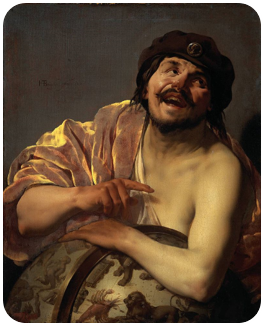
\includegraphics[width=3cm]{DEMOCRITUS}
		\captionof{figure}{Democritus (460 - 370,Hy Lạp)\label{fig:Democritus} }
\end{center}
\end{minipage}

\begin{center}
	\includegraphics[width=12cm]{Historyatom}
	\captionof{figure}{Lịch sử phát triển mô hình nguyên tử \label{fig:Historyatom} }
\end{center}
\end{hoplythuyet}
\subsubsection{Thành phần và cấu trúc của nguyên tử}
\paragraph{Thành phần}
\begin{hoplythuyet}
	Nguyên tử gồm hạt nhân chứa proton, neutron và vỏ nguyên tử chứa electron.
	\begin{center}
		\includegraphics[width=9cm]{mohinhnguyentu}
		\captionof{figure}{Mô hình nguyên tử}
	\end{center}
\end{hoplythuyet}
\paragraph{Sự tìm ra electron}
\ntd{Thí nghiệm khám phá tia âm cực của Thomson}\\
Năm 1897, J.J.Thomson (Tôm-xơn, người Anh) thực hiện thí nghiệm phóng điện qua không khí loãng đã phát hiện ra chùm tia phát ra từ cực âm.(xem hình \ref{fig:tiaamcuc} ) và link video bằng mã QR ở bên dưới.\\ 
\begin{minipage}{0.6\textwidth}
\begin{center}
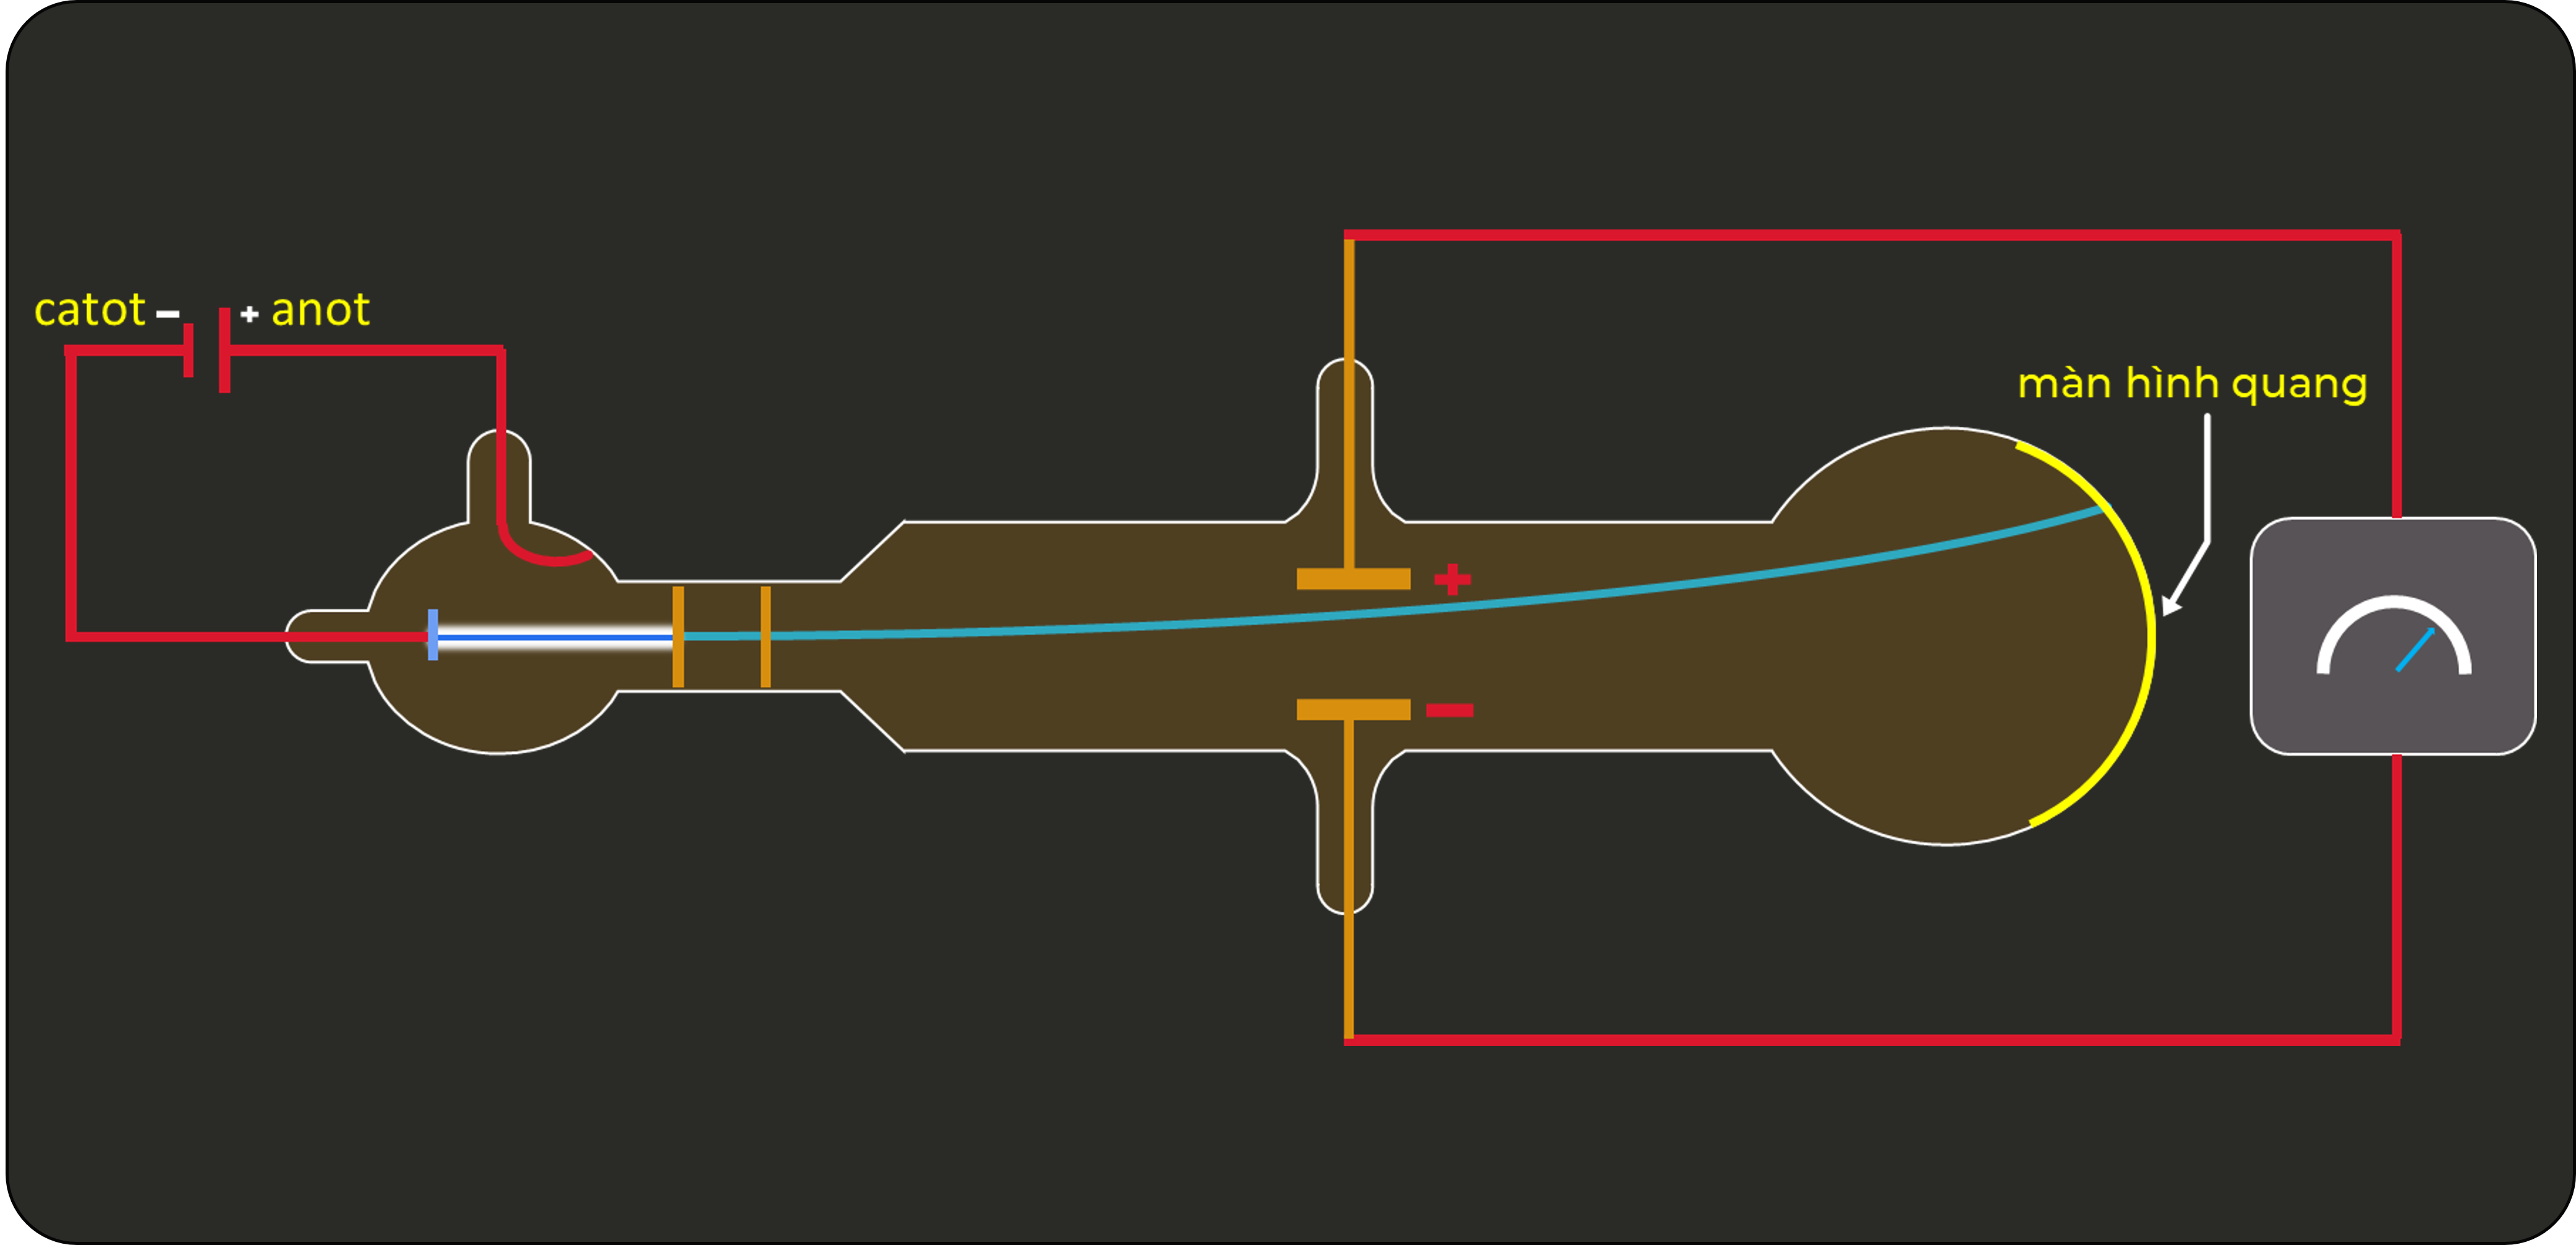
\includegraphics[width=9cm]{TNTHOMSON}\\
\captionof{figure}{Thí nghiệm của Thomson}
\label{fig:tiaamcuc}
\end{center}
\end{minipage}
\hfill
\begin{minipage}{0.3\textwidth}
\begin{tikzpicture}
\path (0,0)  node (QRCODE) {\qrcode[height=2.0cm]{https://youtu.be/y2uswXtC5O8}}
(QRCODE.south) node[anchor=north]{(\fmmfamily Các bạn  dùng ~\rotatebox{-15}{\faMobile}~quét mã QR để xem video TN nhé!)}
;
\end{tikzpicture}
\end{minipage}
\begin{hoivadap}
	Vai trò của lớp bột huỳnh quang trong thí nghiệm ở hình \ref{fig:tiaamcuc}
	\huongdan{\taodongke{10}}
\end{hoivadap}
%
\begin{hoivadap}
Quan sát Hình \ref{fig:tiaamcuc} và video , giải thích vì sao tia âm cực bị hút về cực dương của trường điện.
	\huongdan{\taodongke{10}}
\end{hoivadap}
%
\begin{hoivadap}
	Nếu đặt một chong chóng nhẹ trên đường đi của tia âm cực thì chong chóng sẽ quay. Từ hiện tượng đó, hãy nêu kết luận về tính chất của tia âm cực.
	\huongdan{\taodongke{5}}
\end{hoivadap}
\newpage
\vspace*{6pt}
\begin{emcobiet}
	 Mô hình Thomson còn gọi là mô hình \lq\lq bánh pudding mận".Theo Thomson:
	\begin{enumerate}
		\item Nguyên tử là quả cầu mang điện tích dương, bên trong chứa các êlectron.
	    \item Nguyên tử trung hòa về điện.
	\end{enumerate}
\end{emcobiet}
%
%
\paragraph{Sự khám phá hạt nhân nguyên tử}
\ntd{Tìm hiểu thí nghiệm của Rutherford}\\
Năm 1911, E. Rutherford (Ro-dơ-pho, người Niu Di-lân) thực hiện thí nghiệm bắn phá lá vàng rất mỏng bằng chùm hạt $ \alpha $ \footnote{Hạt $\alpha$ : hạt nhân helium, mang điện tích dương.} (xem hình \ref{fig:hinh4})
\begin{center}
		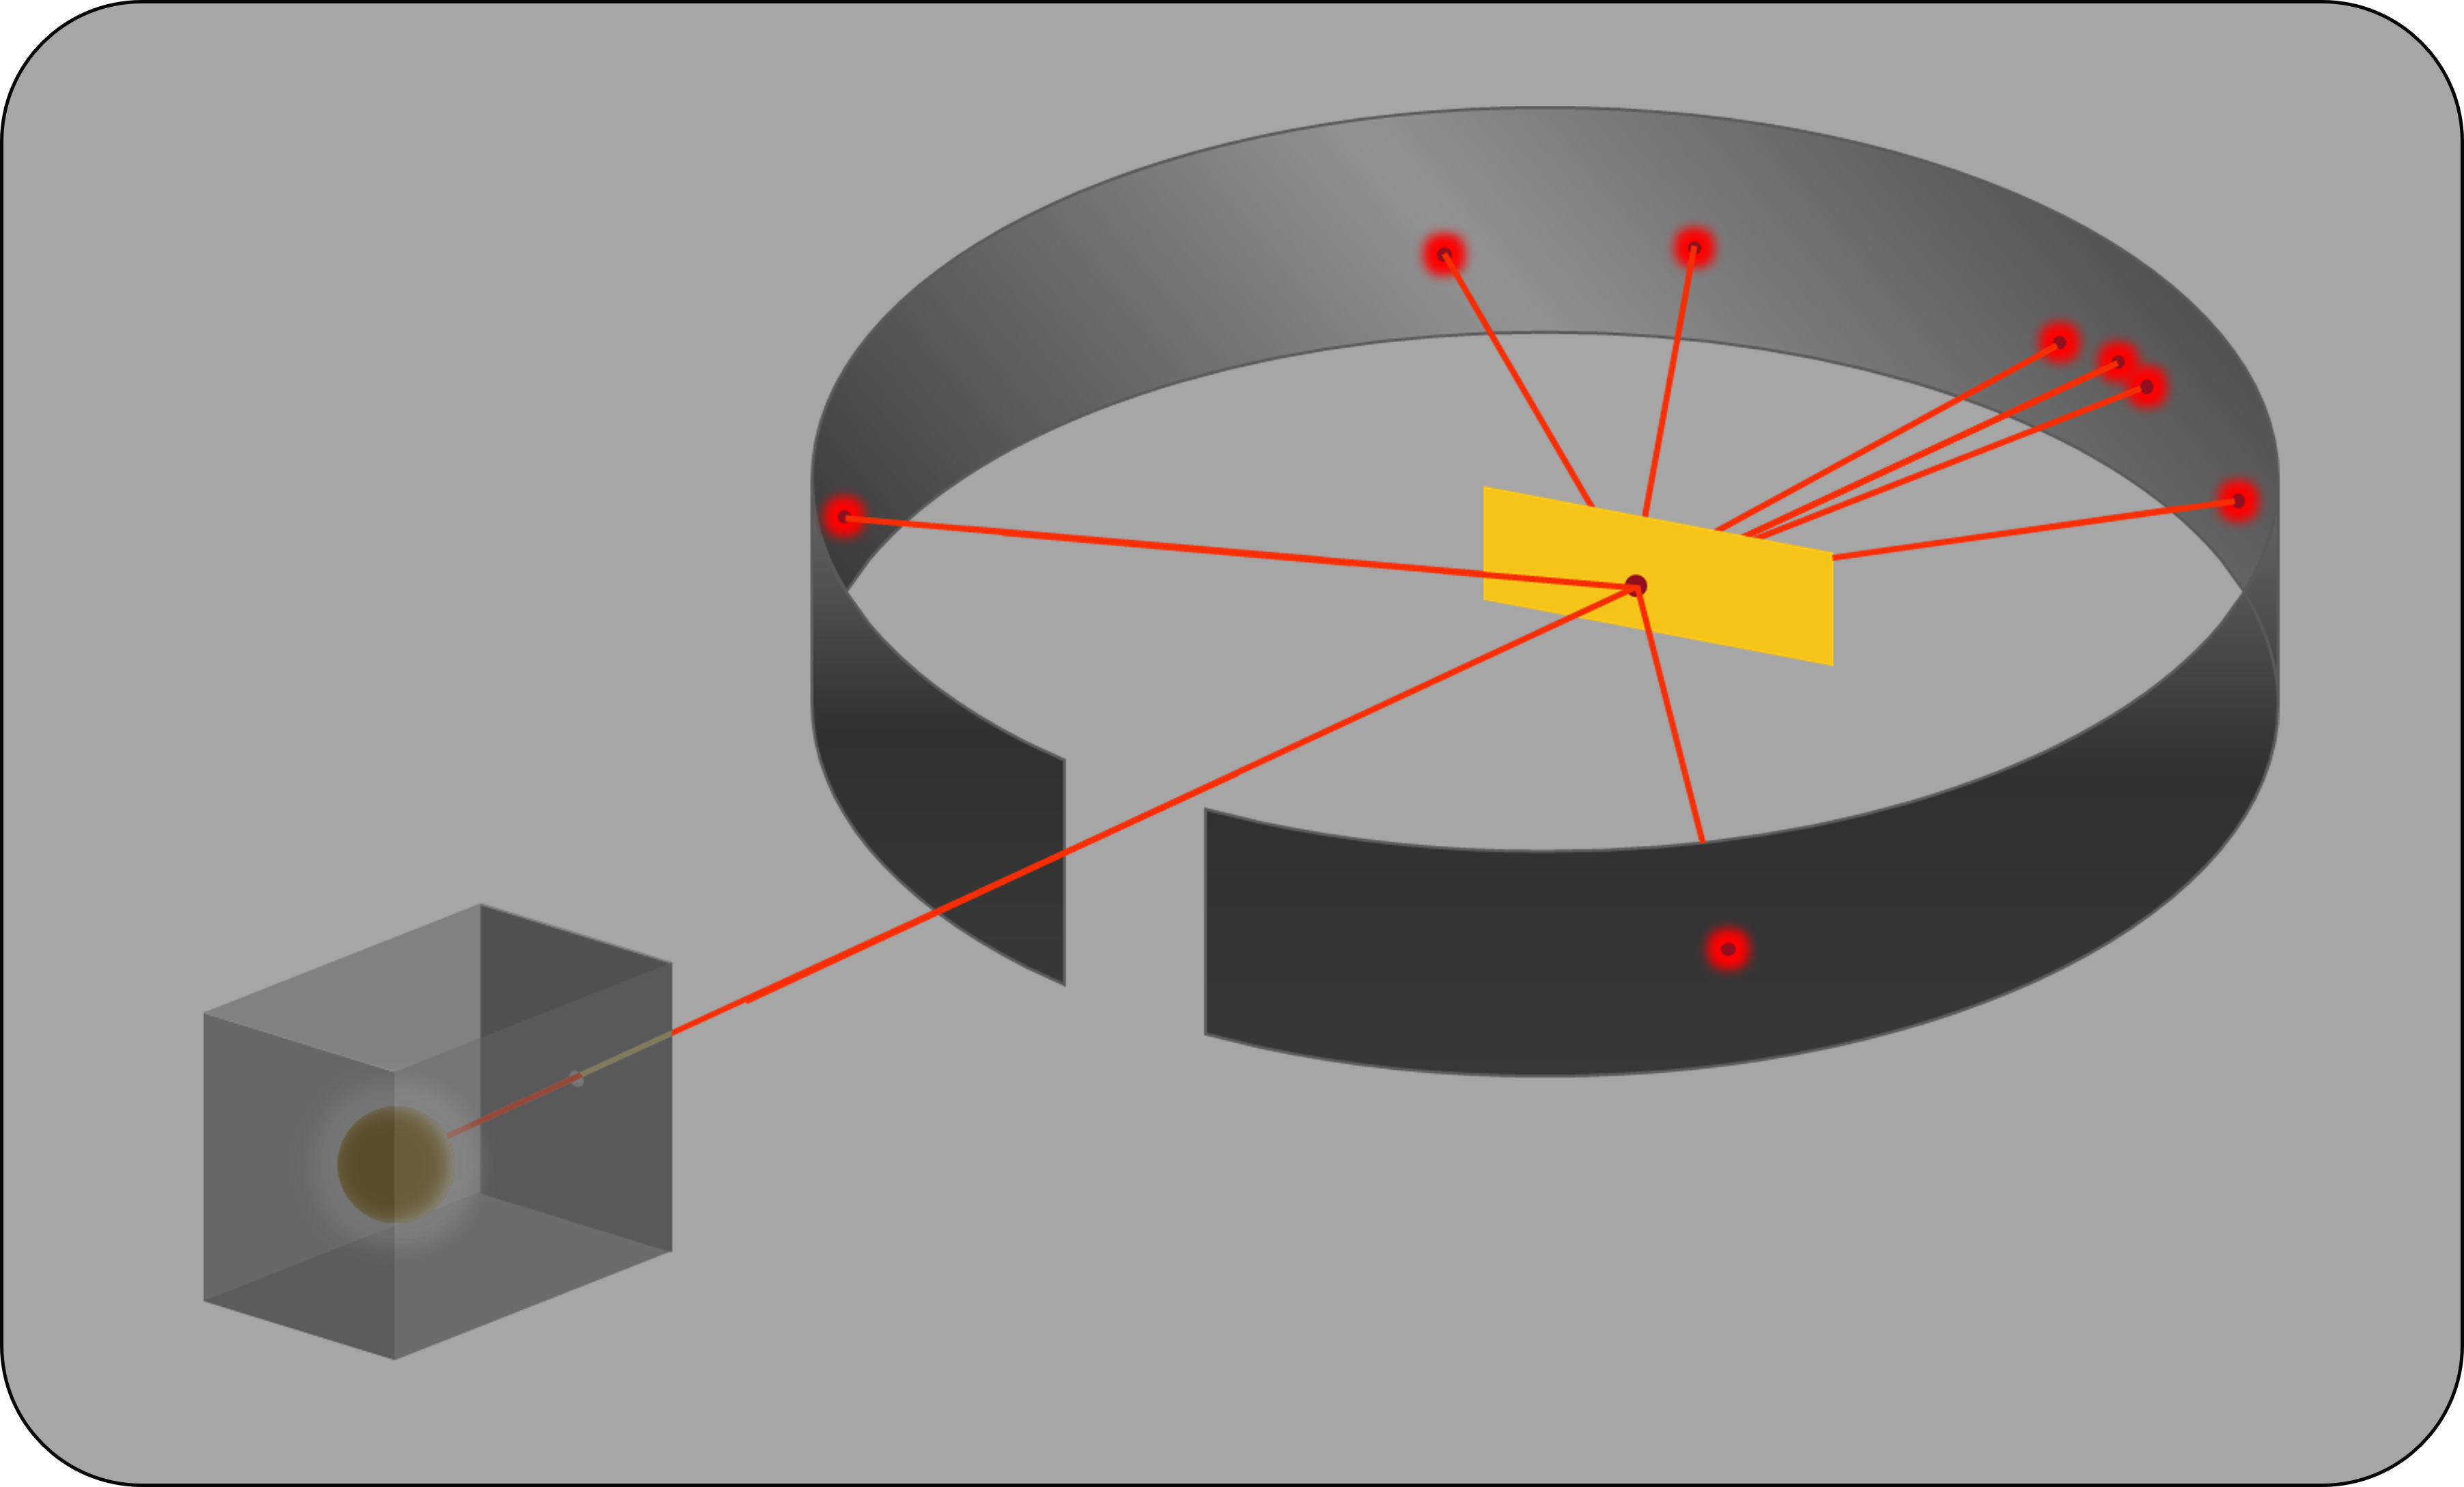
\includegraphics[width=9cm]{TNRUTHERFORT}\\
		\captionof{figure}{Thí nghiệm của Rutherford}
		\label{fig:hinh4}
\end{center}
%
\begin{center}
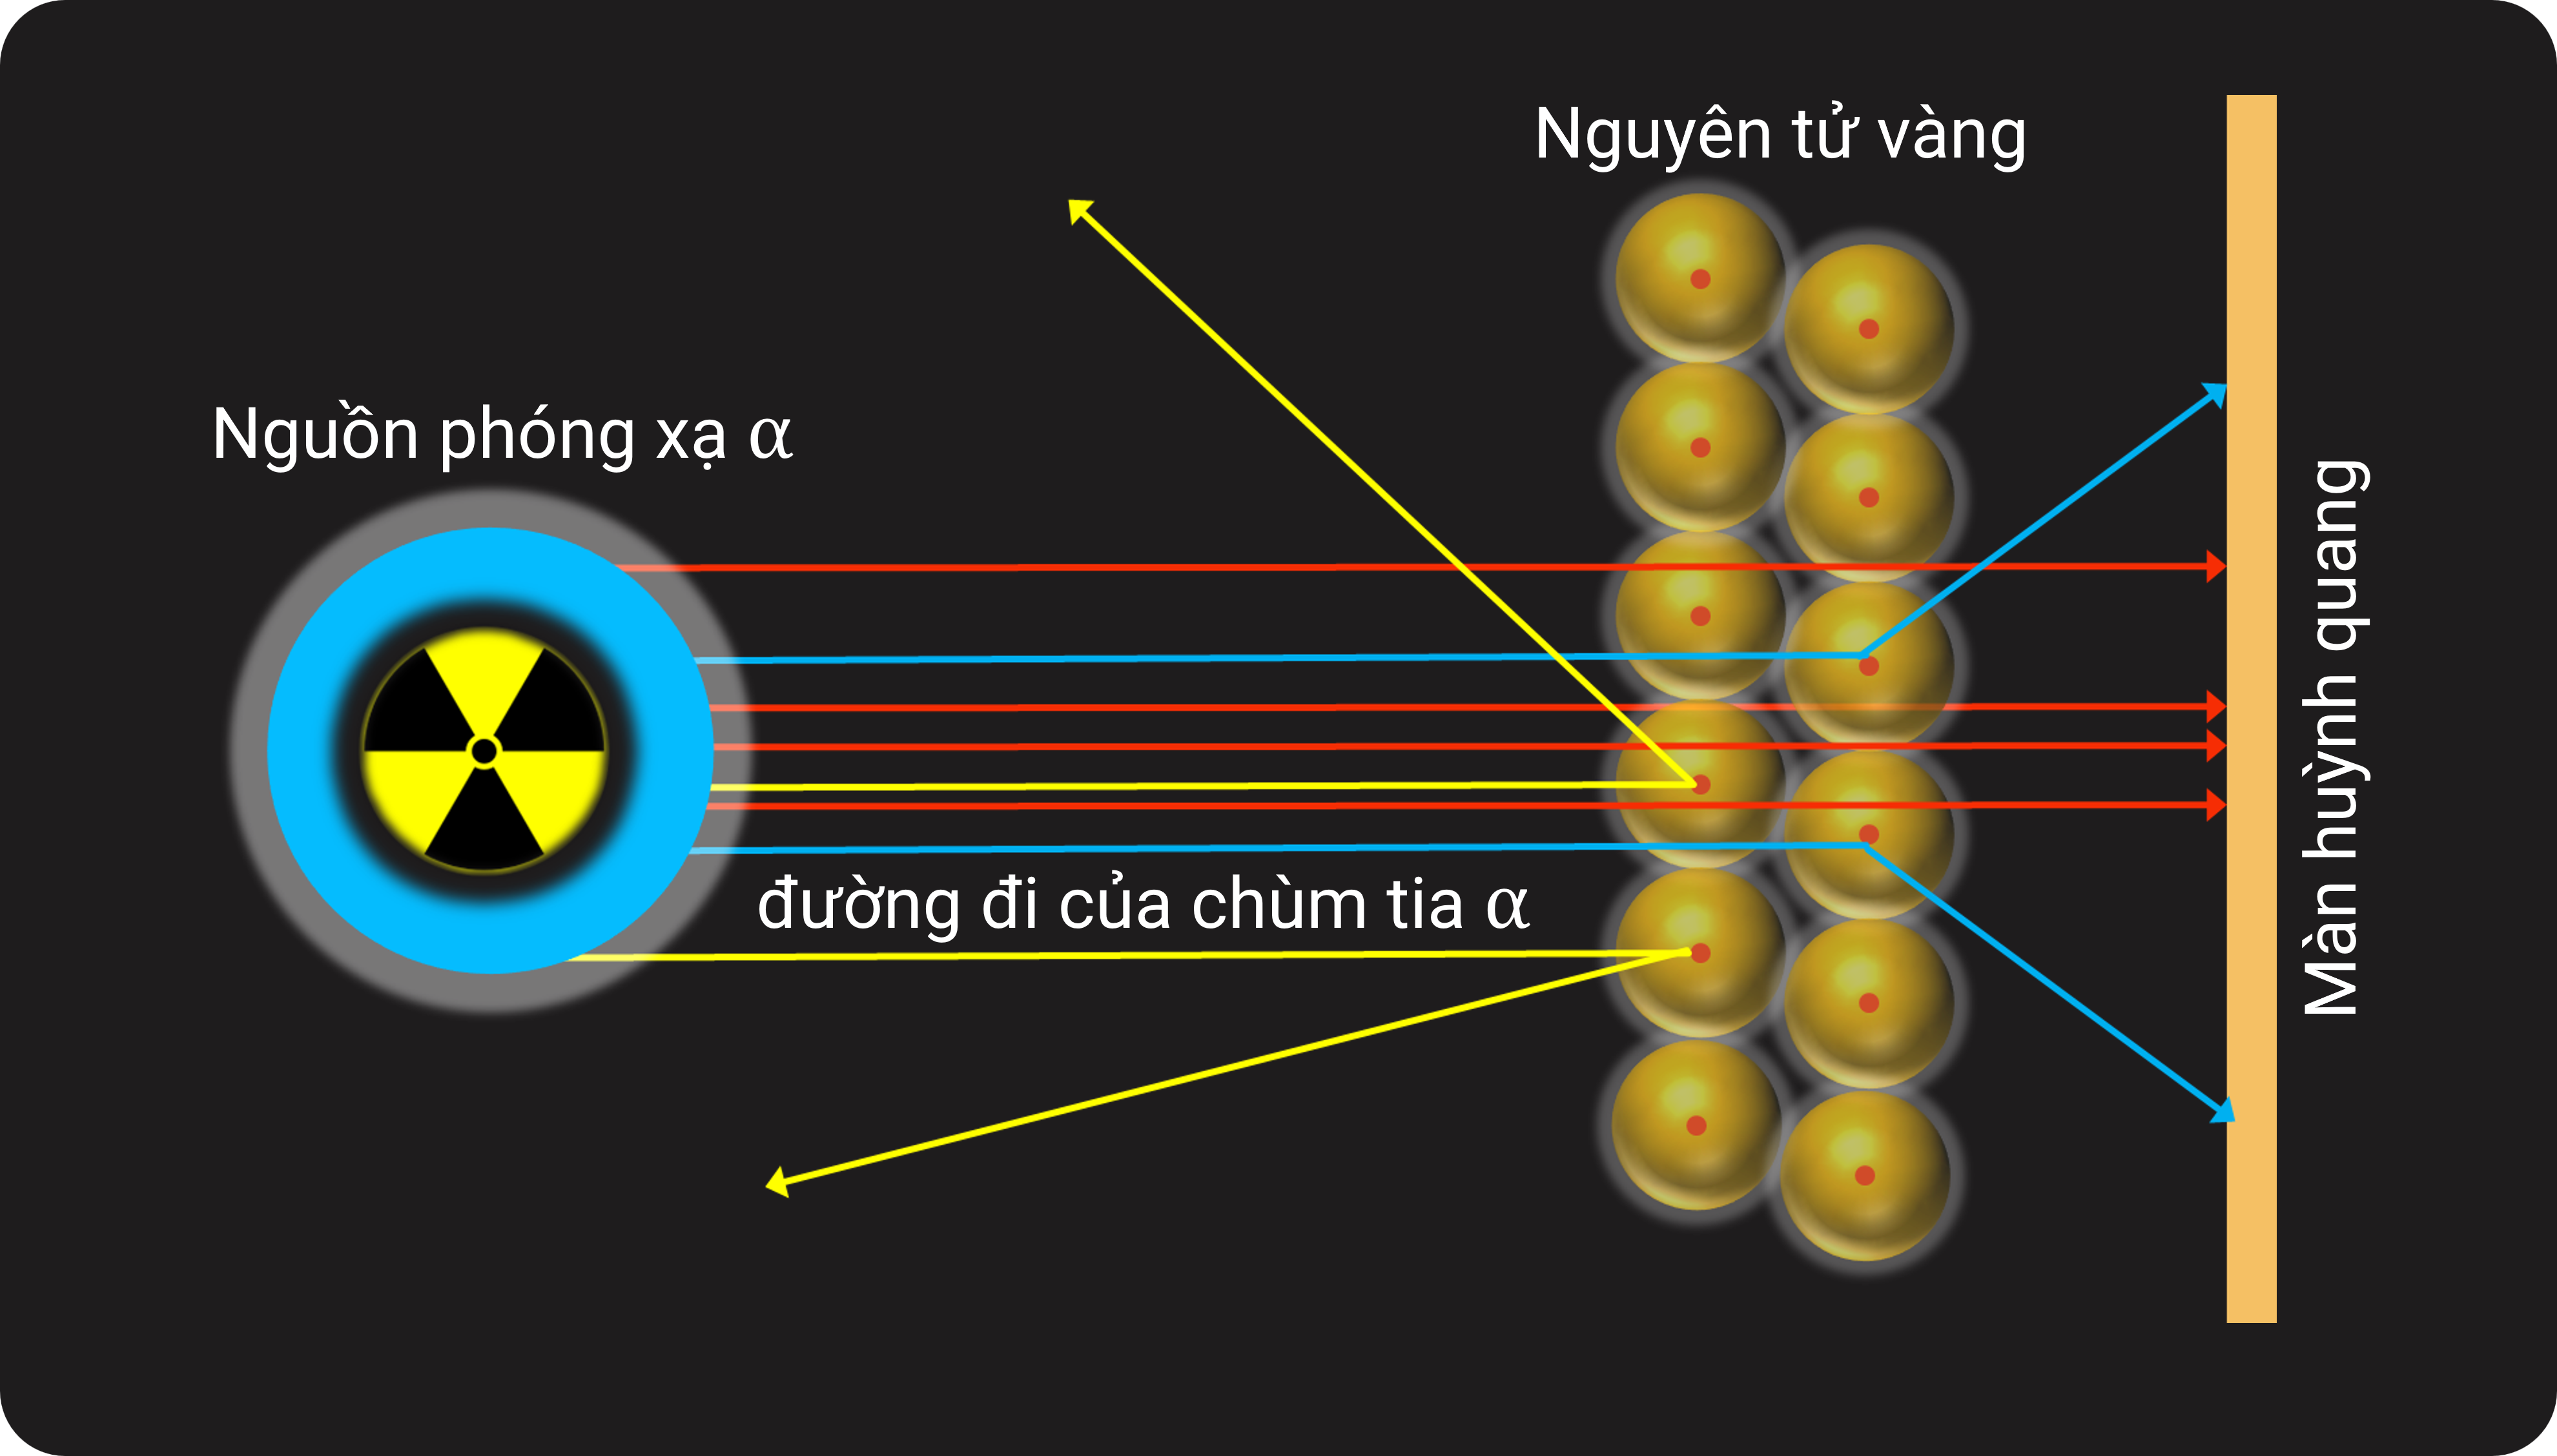
\includegraphics[width=9cm]{KQTN}\\
\captionof{figure}{Kết quả thí nghiệm của Rutherford}
\label{fig:hinh5}
\end{center}
%
\begin{hoivadap}
	Quan sát hình \ref{fig:hinh4}, cho biết các hạt $\alpha$ có đường đi như thế nào. Dựa vào Hình \ref{fig:hinh5} , giải thich kết quả thí nghiệm thu được.
	\huongdan{\taodongke{5}}
\end{hoivadap}
\vspace*{6pt}
\begin{hoplythuyet}
	{\bfseries{Kết luận}}
	\begin{itemize}
	\item Nguyên tử có cấu tạo rỗng, gồm hạt nhân ở trung tâm và lớp vỏ là các electron chuyển động xung quanh hạt nhân.
	\item Nguyên tử trung hoà về điện: số đơn vị điện tích dương của hạt nhân bằng số đơn vị điện tích âm của các electron trong nguyên tử.
	\end{itemize}
\end{hoplythuyet}
\paragraph{Cấu tạo hạt nhân nguyên tử}
\begin{center}
	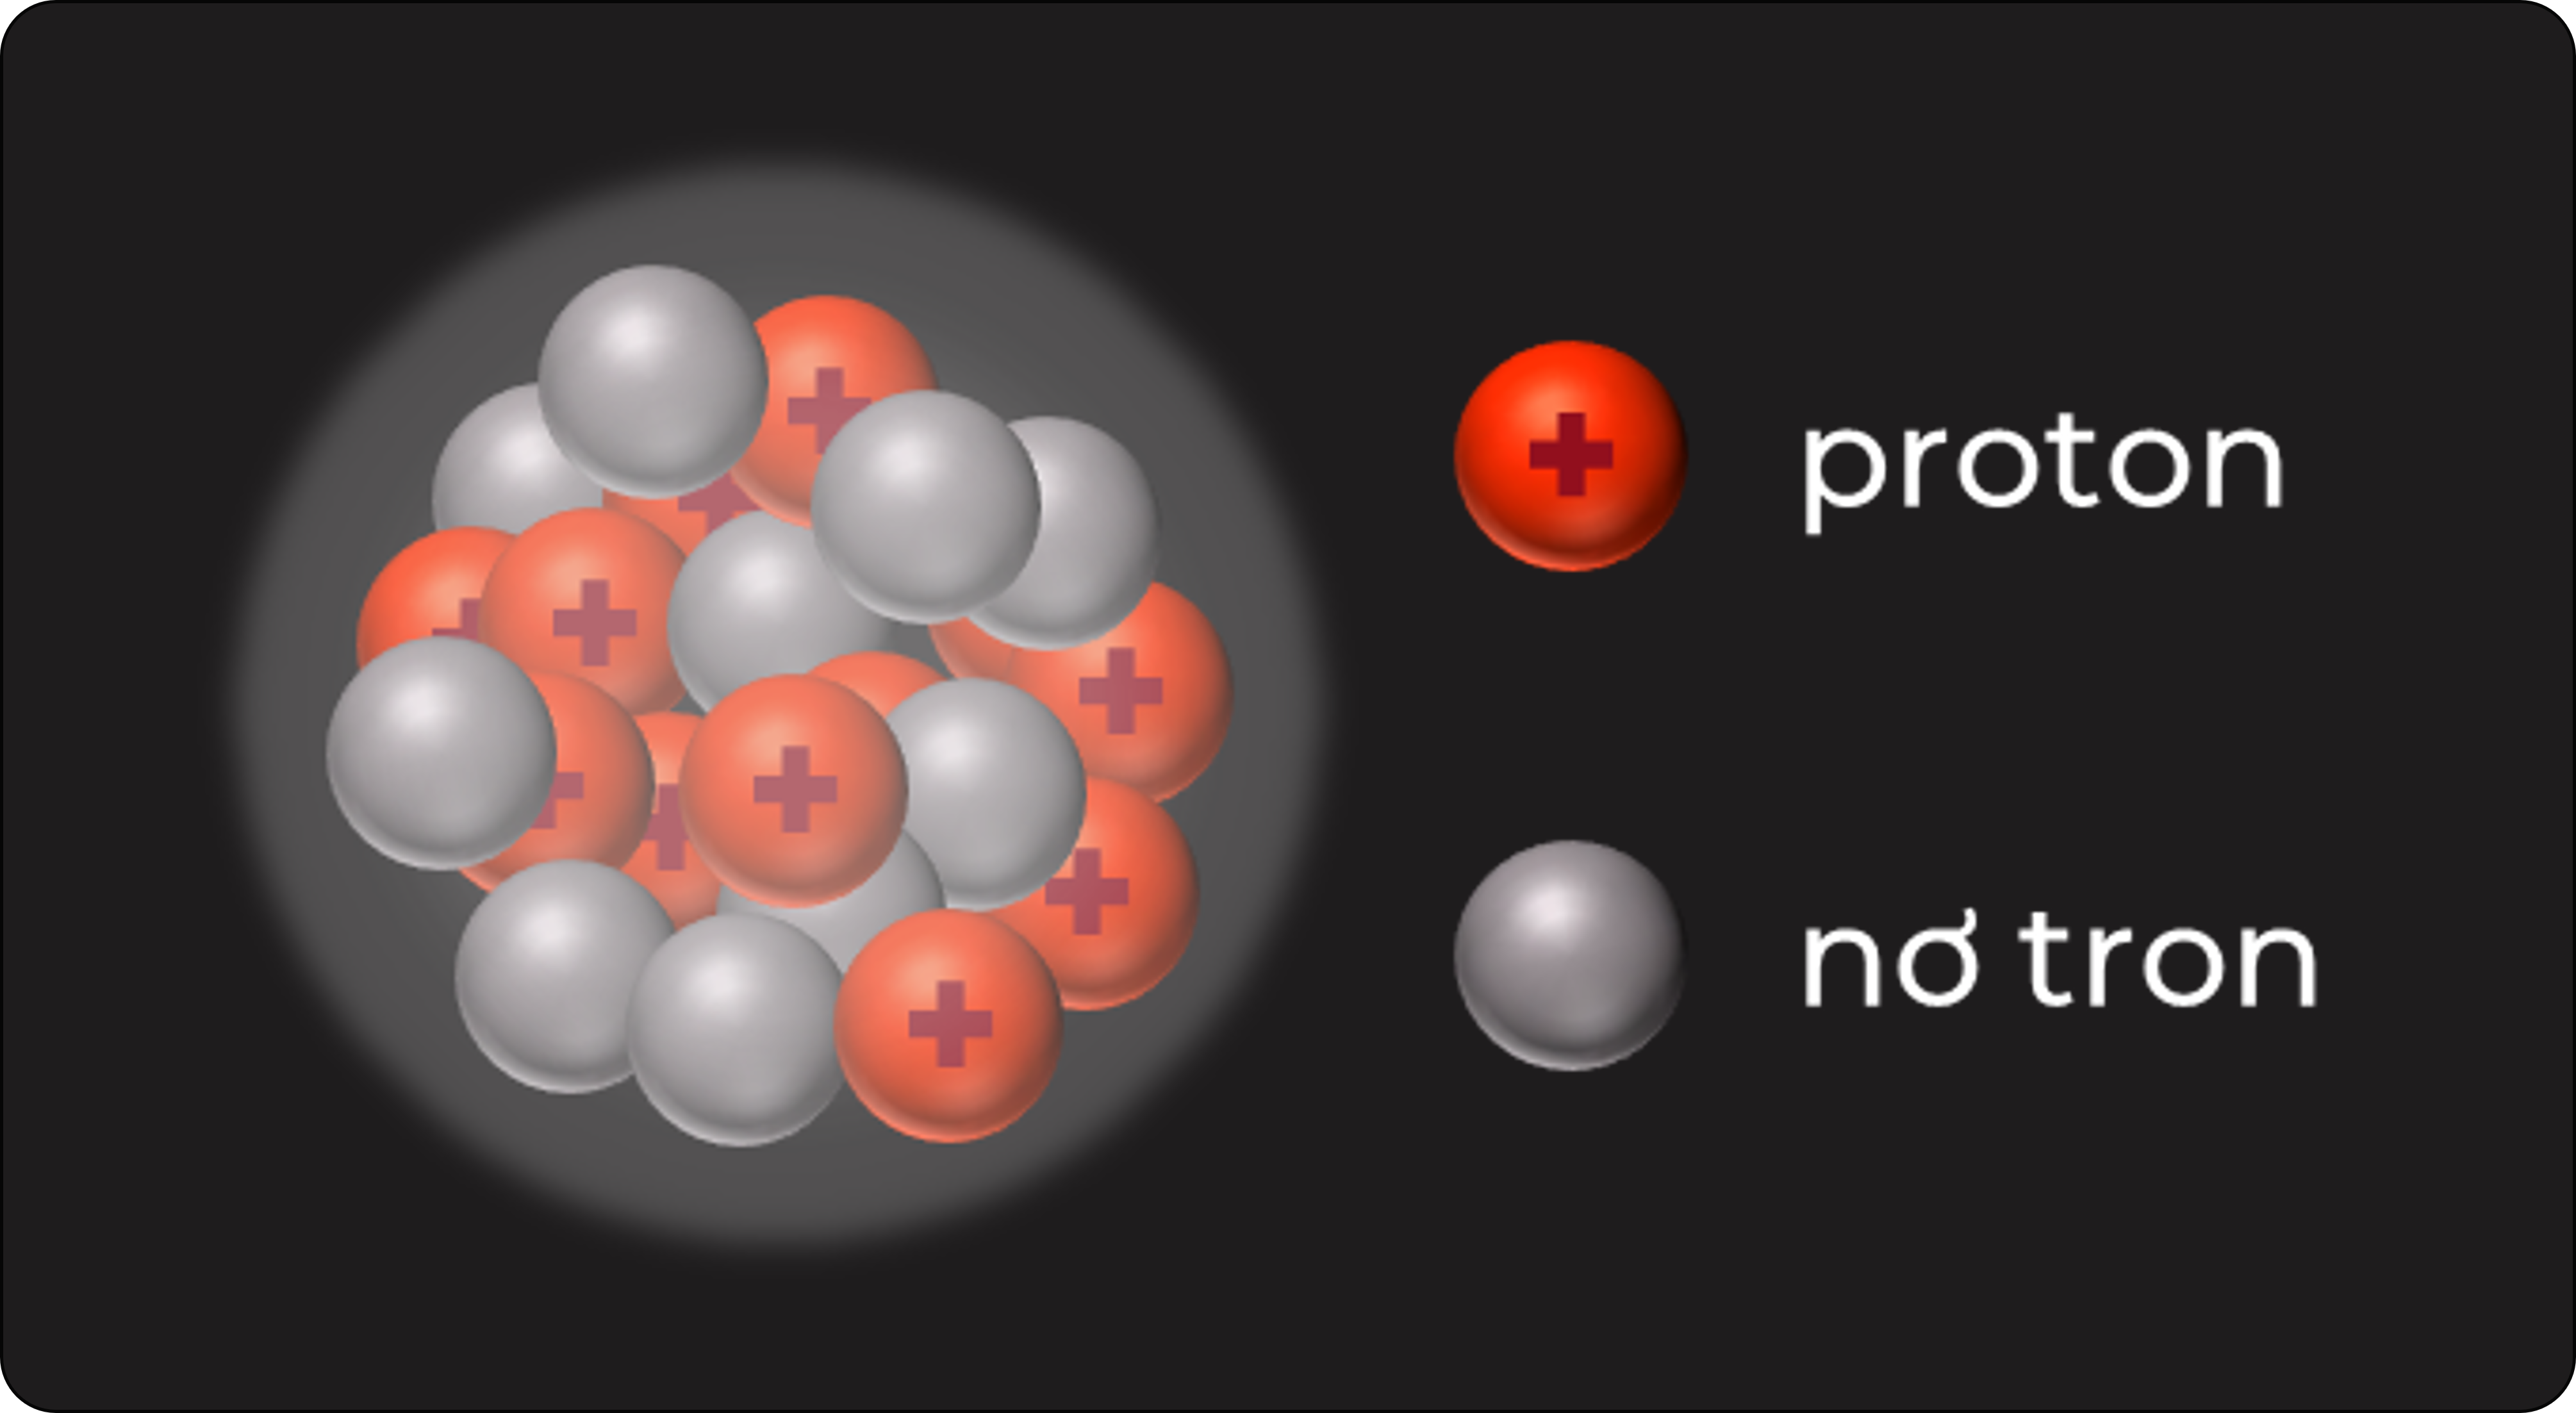
\includegraphics[width=9cm]{CAUTAOHATNHAN}\\
	\captionof{figure}{Thành phần của hạt nhân}
	\label{fig:hinh6}
\end{center}
\begin{hoivadap}
	Quan sát hình \ref{fig:hinh6} và kết hợp SGK , các bạn hãy nêu thành phần của hạt nhân
\end{hoivadap}
\begin{hoplythuyet}
	Proton, neutron và electron là các hạt cấu tạo nên nguyên tử.
\end{hoplythuyet}
\begin{tongket}
	Thành phần cấu tạo của nguyên tử gồm:
\begin{itemize}
	\item  Hạt nhân (nucleus): ở tâm của nguyên tử, chứa các proton mang điện tích dương và các neutron không mang điện.
	\item Vỏ nguyên tử: chứa các electron mang điện tích âm, chuyển động rất nhanh xung quanh hạt nhân.
	\item Trong nguyên tử, số proton bằng số electron nên nguyên tử trung hoà điện.
	\item Khối lượng của electron rất nhỏ, không đáng kể so với khối lượng của proton hay neutron nên khối lượng của nguyên tử tập trung hầu hết ở hạt nhân.
\end{itemize}
\end{tongket}


\begin{longtable}{|c|c|c|c|c|c|}
		\caption{\indam[\maunhan]{Khối lượng, điện tích của các loại hạt cấu tạo nên nguyên tử}}
		\label{tab:table1}\\
\hline
\rowcolor{dnxanh!25} \indam[dnxanh]{Hạt} & \indam[dnxanh]{Kí hiệu} & $\begin{array}{c}\text {\indam[dnxanh]{Khối lượng} } \\
		\text {\indam[dnxanh]{(kg)}  }\end{array}$ & \indam[dnxanh]{Khối lượng (amu)} & $\begin{array}{c}\text { \indam[dnxanh]{Điện tích} } \\
		\text { \indam[dnxanh]{(C)} }\end{array}$ & $\begin{array}{l}\text { \indam[dnxanh]{Điện tích} } \\
		\text { \indam[dnxanh]{tương đối} }\end{array}$ \\
\hline\endhead
\rowcolor{dnvang!15} Proton & $p$ & $1,672 \cdot 10^{-27}$ & $\approx 1$ & $1,602 \cdot 10^{-19}$ & +1 \\
\hline
\rowcolor{dnvang!15} Neutron & $\mathrm{n}$ & $1,675 \cdot 10^{-27}$ & $\approx 1$ & 0 & 0 \\
\hline\rowcolor{dnvang!15} Electron & e & $9,109 \cdot 10^{-31}$ & $\begin{array}{c}
		~ \\
		\dfrac{1}{1837} \approx 0,00055\\
		~ \\
	\end{array}$ & $-1,602 \cdot 10^{-19}$ & -1 \\
	\hline
	\end{longtable}
\paragraph{KíCH THƯỚC VÀ KHỐI LƯợNG NGUYÊN TỬ}
\begin{center}
	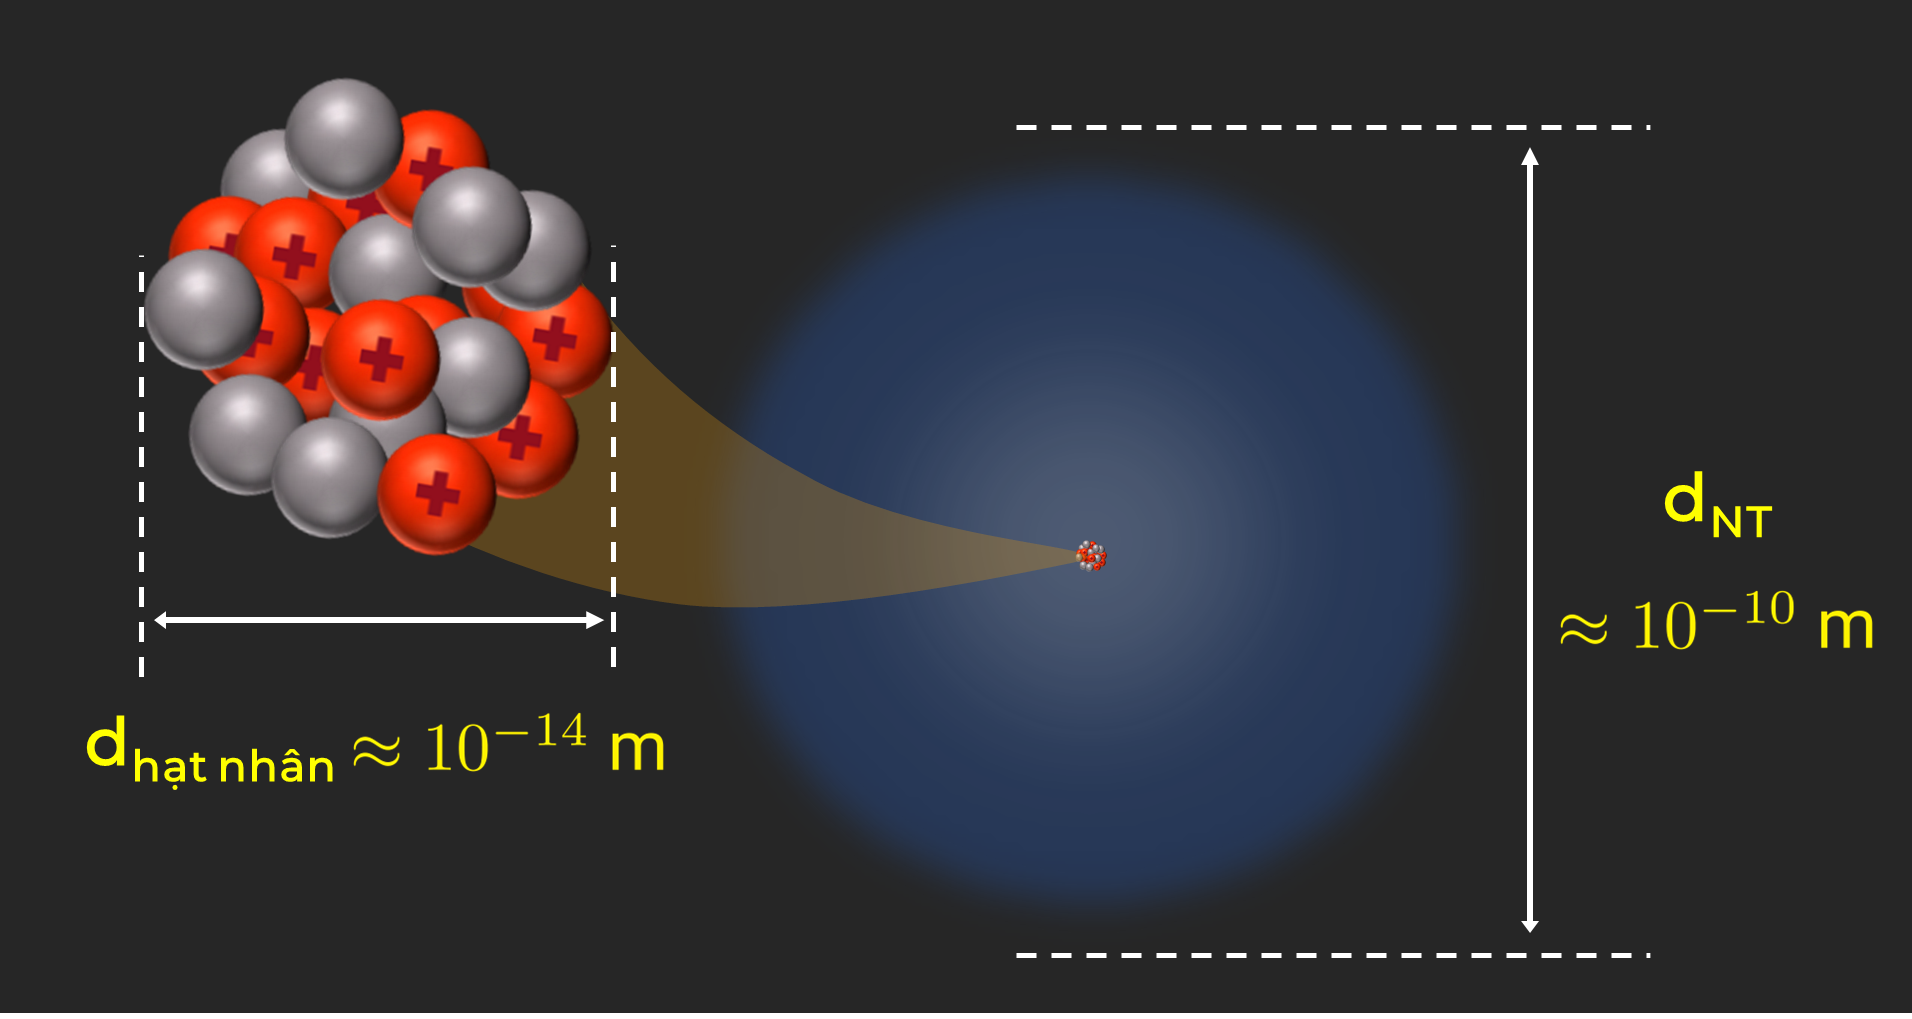
\includegraphics[width=9cm]{ktnt}\\
	\captionof{figure}{So sánh kích thước hạt nhân , nguyên tử}
	\label{fig:hinh7}
\end{center}
\begin{notegsnd}
		\begin{itemize}
\item Đơn vị kích thước thường dùng của nguyên tử là Angstron ($ A^0 $) hoặc nano mét (nm)			
	$$1 \mathrm{~nm}=10^{-9}~\mathrm{m} ; 1 A^0=10^{-10}~\mathrm{~m} ; 1 \mathrm{~nm}=10 A^0; 1 A^0=10^{2}~\mathrm{pm}$$
	\begin{center}
	\tcbox[width=5cm,colframe=\maunhan]{$ \dfrac{d_{\text{NT}}}{d_{\text{hạt nhân}}}\approx \dfrac{10^{-10}}{10^{-14}} \approx 10^4~\mathrm{\text{lần}} $}
	\end{center}
		\item Đơn vị của khối lương nguyên tử là amu (atomic mass unit),
		$$
		1 \mathrm{amu}=1,6605 \times 10^{-27} \mathrm{~kg} \text {. }
		$$
		\item Đơn vi của điện tích các hạt cơ bản là $\mathrm{e}_0$ (điện tích nguyên tố),
		$$
		1 \mathrm{e}_0=1,602 \times 10^{-19} \mathrm{C} \text {. }
		$$
	\end{itemize}
\end{notegsnd}
\newpage
\vspace*{3pt}

\ntd{BÀI TẬP TRẮC NGHIỆM}:
\begin{dangntd}{LÝ THUYẾT VỀ CẤU TẠO NGUYÊN TỬ}
\giaibaitap{Phương pháp giải}
\begin{itemize}
	\item Nắm vững về cấu tạo nguyên tử
	\item Nắm vững kết quả thí nghiệm của Thomson,Rutherford
\end{itemize}
\end{dangntd}
\Opensolutionfile{ansbook}[DAPAN/BTTLH10CO102tachLG]
\Opensolutionfile{ans}[DAPAN/BTTLH10CO102]
\begin{ex}[1]
	Các hạt cơ bản của hầu hết các nguyên tử là?
	\choice
{%
electron
}
{%
	electron và proton
}
{%
 proton và notron
}
{%
\True electron, proton và notron
}
%\sodongkeex[5]
\huongdan{

}
\end{ex}


\begin{ex}[1]
	Hạt nhân của hầu hết các nguyên tử gồm có?
	\choice
	{%
		electron
	}
	{%
		electron và proton
	}
	{%
	\True proton và notron
	}
	{%
		 electron, proton và notron
	}
%\sodongkeex[5]
\huongdan{
	
}
\end{ex}

\begin{ex}[2]
Trong thí nghiệm của Thomson, phát biểu nào sau đây sai với kết quả thí nghiệm ta quan sát được?
	\choice
{%
 Tia âm cực là các chùm hạt electron di chuyển từ cực âm sang cực dương
}
{%
	Tia âm cực là chùm hạt mang điện tích âm
}
{%
\True	Tia âm cực bị lệch về phía bản cực âm của nguồn điện
}
{%
	Tia âm cực bị lệch hướng khi ta đặt nó trong từ trường
}
%\sodongkeex[5]
\huongdan{
	
}
\end{ex}

\begin{ex}[2]
Theo mô hình bánh pudding mận của Thomson, phát biểu nào sau đây là đúng?
\choice
{%
Nguyên tử có cấu tạo rỗng gồm hạt nhân mang điện tích dương và vỏ là các electron chuyển động xung quanh hạt nhân.
}
{%
Nguyên tử có cấu tạo rỗng gồm hạt nhân mang điện tích dương và vỏ là các electron chuyển dộng xung quanh hạt nhân theo những quỹ đạo có kích thước và năng lượng cố định
}
{%
\True	nguyên tử bao gồm các electron nằm rải rác trong một đám mây hình cầu mang điện tích dương.
}
{%
	các electron  quay quanh hạt nhân không theo một quỹ đạo xác định, mà chúng tạo thành các đám mây điện tích mà tại đó xác suất tìm thấy electron là lớn nhất
}
%\sodongkeex[5]
\huongdan{
	
}
\end{ex}
\begin{ex}[2]
Cho các phát biểu sau:
\begin{enumerate}[(1)]
\item Tất cả các hạt nhân nguyên tử đều được cấu tạo từ các hạt proton và neutron.
\item Khối lượng nguyên tử tập trung phần lớn ở lớp vỏ.
\item Trong nguyên tử, số electron bằng số proton.
\item Trong hạt nhân nguyên tử, hạt mang điện là proton và electron.
\item Trong nguyên tử, hạt electron có khối lượng không đáng kể so với các hạt còn lại.
\end{enumerate}
Số phát biểu đúng là
\choice
{%
	1
}
{%
\True 2
}
{%
3
}
{%
4
}
\huongdan{%
Phát biểu đúng là:
Trong hạt nhân nguyên tử, hạt mang điện là proton và electron.\\
Trong nguyên tử, hạt electron có khối lượng không đáng kể so với các hạt còn lại
}

\end{ex}

\begin{ex}[2]
Điều nào sau đây đúng theo mô hình nguyên tử của Thomson?
\choice
{%
Nguyên tử không trung hòa về điện
}
{%
\True Nguyên tử là quả cầu mang điện tích dương có chứa các êlectron bên trong
}
{%
Điện tích âm và điện tích dương trong nguyên tử có độ lớn bằng nhau
}
 {%
 Không có điều nào ở trên
 }
%\sodongkeex[5]
\huongdan{
	
}
\end{ex}


\begin{ex}[3]
	Trong hiện tượng xả điện qua khí ở áp suất thấp, sự tỏa sáng màu trong ống xuất hiện là kết quả của:
	\choice
	{% 
\True va chạm giữa các hạt mang điện được phát ra từ cực âm và nguyên tử của khí
	}
{% 
	va chạm giữa các electron khác nhau của các nguyên tử trong khí
}
{% 
	kích thích các electron trong các nguyên tử
}	
{% 
va chạm giữa các nguyên tử của khí
}	
%\sodongkeex[5]
\huongdan{
	
}	
\end{ex}

\begin{ex}[2]
Mô hình đầu tiên về nguyên tử được đưa ra bởi:
\choice
{%
N. Bohr
}
{% 
	E. Goldstein
}
{% 
	Rutherford
}
{% 	
\True J.J. Thomson
}
%\sodongkeex[5]
\huongdan{
	
}
\end{ex}

\begin{ex}[2]
Nếu đường kính của nguyên tử khoảng $10^2 \mathrm{pm}$ thì đường kính của hạt nhân khoảng
\choice
{%
$10^2 \mathrm{pm}$
}
{%
$10^{-4} \mathrm{pm}$
}
{%
\True	$10^{-2} \mathrm{pm}$
}
{
$10^4 \mathrm{pm}$
}
%\sodongkeex[5]
\huongdan{
	
}
\end{ex}
\Closesolutionfile{ans}
\Closesolutionfile{ansbook}


\newpage
\giaibaitap{BÀI TẬP TỰ LUẬN}
\Opensolutionfile{ansbt}[DAPAN/BT_H10C0102]
\begin{btex}[2]
	Trong thí nghiệm của Rutherford, khi sử dụng các hạt alpha (ion $\mathrm{He}^{2+}$, kí hiệu là $\mathrm{a}$ ) bắn vào lá vàng thì:
	\begin{itemize}
	\item Hầu hết các hạt a xuyên thẳng qua lá vàng.
	\item Một số ít hạt a bị lệch quỹ đạo so với ban đầu.
	\item Một số rất ít hạt a bị bật ngược trở lại.
	\end{itemize}
	Từ kết quả này, em có nhận xét gì về cấu tạo nguyên tử?
	\loigiai{
	Trong thí nghiệm của Rutherford, khi sử dụng các hạt alpha (ion $\mathrm{He}^{2+}$, kí hiệu là a) bắn vào lá vàng thì:
	\begin{itemize}
	\item Hầu hết các hạt a xuyên thẳng qua lá vàng chứng tỏ nguyên tử có cấu tạo rỗng.
	\item Một số ít hạt a bị lệch quỹ đạo so với ban đầu chứng tỏ hạt nhân nguyên tử cùng điện tích dương như hạt hạt alpha (ion $\mathrm{He}^{2+}$, kí hiệu là $ \alpha $).
	\item Một số rất ít hạt a bị bật ngược trở lại chứng tỏ kích thước hạt nhân nhỏ hơn rất nhiều so với kích thước của nguyên tử và khối lượng nguyên tử tập trung chủ yếu ở hạt nhân.
	\end{itemize}

}
\end{btex}

\begin{btex}[2]
Viết lại bảng sau vào vở và điền thông tin còn thiếu vào các ô trống:\\
\begin{tabular}{|c|c|c|c|c|c|c|}
\rowcolor{dnxanh!25} 
\hline \indam[dnxanhdam]{Nguyên tố} & \indam[dnxanhdam]{Kí hiệu} & \color{dnxanhdam} {$\mathbf{Z}$} & \indam[dnxanhdam]{Số e} & \indam[dnxanhdam]{Số p} & \indam[dnxanhdam]{Số n} & \indam[dnxanhdam]{Số khối} \\
\rowcolor{dnvang!25} 
\hline \indam[dnxanhdam]{Carbon} & $\mathrm{C}$ & 6 & 6 & $?$ & 6 & $?$ \\
\rowcolor{dnvang!25} 
\hline \indam[dnxanhdam]{Nitrogen} & $\mathrm{N}$ & 7 & $?$ & 7 & $?$ & 14 \\
\rowcolor{dnvang!25} 
\hline \indam[dnxanhdam]{Oxygen} & $\mathrm{O}$ & 8 & 8 & $?$ & 8 & $?$ \\
\rowcolor{dnvang!25} 
\hline \indam[dnxanhdam]{Sodium (natri)} & $\mathrm{Na}$ & 11 & $?$ & 11 & $?$ & 23 \\
\rowcolor{dnvang!25}
\hline \indam[dnxanhdam]{Aluminium (nhôm)} & $\mathrm{Al}$ & $?$ & 13 & $?$ & $?$ & 27 \\
\hline
\end{tabular}
\huongdan{
\taodongke{5}
}
\end{btex}

\Closesolutionfile{ansbt}

\newpage
\begin{dangntd}{Bài tập về khối lượng, kích thước nguyên tử}	
	\giaibaitap{Phương pháp giải}\\
	\tieumuc{Các công thức liên quan khối lượng}
	\begin{itemize}
		\item $ m _{\text{nguyên tử}=m_{p}+m_{n} + m_{e} } $ (tính chính xác); $ m _{\text{nguyên tử}} \approx  m_{p} + m_{n} \approx m_{\text{hạt nhân}} $ (tính gần đúng)
		\item Khối lượng tính ra kg của 1 nguyên tử carbon-12 là $ 19,926 . 10^{27}~\mathrm{kg}$.
		\item 1 amu được định nghĩa bằng $\dfrac{1}{12}$ khối lượng 1 nguyên tử carbon-12:
		\item$1 \mathrm{amu}=\dfrac{19,926 \cdot 10^{-27} \mathrm{~kg}}{12}=1,661 \cdot 10^{-27} \mathrm{~kg}$
		\item$1 \mathrm{mol}$ chứa $ 6,02.10^{23} $ nguyên tử, phân tử, ion.
	\end{itemize}
	\tieumuc{Các công thức liên quan kích thước}
	\begin{itemize}
		\item Thể tích của hình cầu:
		$ V=\dfrac{4}{3}\pi r^3 $
		\item Phần trăm thể tích các nguyên tử trong tinh thể $ = \dfrac{V_{\text{các nguyên tử}}}{V_{\text{tinh thể}}}\cdot 100\% $
		\item Một số đơn vị đo: 
		$\left\{\begin{array}{l}
			1~\mathrm{nm} = 10^{-9}~\mathrm{m}\\
			1~\mathrm{A^{0}} = 10^{-10}~\mathrm{m}\\
			1~\mathrm{pm} = 10^{-12}~\mathrm{m}	
		\end{array}\right.$
	\end{itemize}
\end{dangntd}
\begin{vdm}{Ví dụ mẫu}
\end{vdm}

%Câu 1: Khối lượng của nguyên tử magnesium là $39,8271 \cdot 10^{-27} \mathrm{~kg}$. Khối lượng của magnesium theo amu là
%A. 23,978
%B. $66,133 \cdot 10^{-51}$.
%C. 24,000 .
%D. $23,985 \cdot 10^{-3}$.

\begin{vdex}[2]	
	Khối lượng của nguyên tử magnesium là $39,8271 \cdot 10^{-27} \mathrm{~kg}$. Khối lượng của magnesium theo amu là
	\choice
	{%
		\True $ 23,978 $
	}
	{%
		$66,133 \cdot 10^{-51}$
	}
	{%
		$23,985 \cdot 10^{-3}$
	}
	{%
		$ 24,000 $
	}
	\huongdan{
		
	}	
\end{vdex}

\begin{vdex}[2]
	Khối lượng tuyệt đối của một nguyên tử oxygen bằng $26,5595.10^{-27} \mathrm{~kg}$. Hãy tính khối lượng nguyên tử (theo amu) và khối lượng mol nguyên tử (theo g) của nguyên tử này.
	\loigiai
	{%
		$
		1 \mathrm{amu}=1,661 \cdot 10^{-27} \mathrm{~kg}
		$\\
		
		
		Khối lượng của nguyên tử oxygen theo amu là:
		$
		\dfrac{26,5595 \cdot 10^{-27}}{1,661 \cdot 10^{-27}} \approx 15,99~ \mathrm{amu}
		$\\
		
		$1 \mathrm{mol}$ chứa $ 6,02.10^{23} $ nguyên tử\\
		$\Rightarrow$ Khối lượng mol của oxygen là  $=26,5595.10^{-24}.6,02.10^{23}= 15,99~ \mathrm{gam} $
		
	}
\end{vdex}

%Câu 3: Nguyên tử helium có 2 proton, 2 neutron và 2 electron. Khối lượng của các electron chiếm baoo nhiêu $\%$ khối lượng nguyên tử helium?
%A. $2,72 \%$.
%B. $0,272 \%$.
%C. $0,0272 \%$.
%D. $0,0227 \%$.

\begin{vdex}[2]
	Nguyên tử helium có 2 proton, 2 neutron và 2 electron. Khối lượng của các electron chiếm bao nhiêu $\%$ khối lượng nguyên tử helium?
	\choice
{%
	$2,72 \%$
}
{%
	$0,272 \%$
}
{%
\True	$0,0272 \%$
}
{%
	$0,0227 \%$
}
	\huongdan
	{%
		Khối lượng nguyên tử helium là:\\ $ m_{NT} = 2m_{p} + 2m_{n} + 2m_{e} = 2.1,672.10^{-27} + 2.1,675.10^{-27} + 2 .9,109.10^{-31} = 6.696.10^{-27}~\mathrm (kg) $\\
		Phần trăm khối lượng của electron trong nguyên tử helium là:\\
		$ \%m_{e}=\dfrac{2 .9,109.10^{-31}}{5.51941.10^{-27}}.100\%=0,0272 \%$
		
	}
\end{vdex}



\begin{vdex}[2]
	Khối lượng riêng của canxi kim loại  là $ 1,55 g/cm^3 $. Giả thiết rằng , trong tinh thể canxi các nguyên tử là những hình cầu chiếm $ 74\% $ thể tích tinh thể, phần còn lại là khe rỗng.Bán kính nguyên tử tính theo lý thuyết là
	\choice
	{%
		$0,185~\mathrm{nm}$
	}
	{%
	\True	$0,196~\mathrm{nm}$
	}
	{%
		$0,155~\mathrm{nm}$
	}
	{%
		$0,168~\mathrm{nm}$
	}
	\huongdan
	{%
		Lấy 1 mol Ca\\
		Ta có: $ D_{Ca}=\dfrac{m_{Ca}}{V_{\scriptsize\text{tinh thể Ca}}}=\dfrac{M_{Ca}.1}{V_{\scriptsize\text{tinh thể Ca}}}\Rightarrow V_{\scriptsize\text{tinh thể Ca}} = \dfrac{M_{Ca}}{D_{Ca}} ~\mathrm{cm^{3}} $\\
		Thể tích 1 mol ca là: $ V_{\scriptsize\text{ 1 mol Ca} } = \dfrac{74}{100} \cdot V_{\scriptsize\text{tinh thể Ca}} = \dfrac{74}{100} \cdot \dfrac{M_{Ca}}{D_{Ca}} $\\
		Thể tích một nguyên tử Canxi là:
		$V_{\scriptsize\text{1 NT Ca}} = \dfrac{V_{\scriptsize\text{ 1 mol Ca}}}{6,02.10^{23}}=\dfrac{74.M_{Ca}}{6,02.10^{23}.100.D_{Ca}} $\\
		$ \Rightarrow \dfrac{4}{3}\pi r^{3} = \dfrac{74.M_{Ca}}{6,02.10^{23}.100.D_{Ca}} \Rightarrow \dfrac{4}{3}\pi r^{3} = \dfrac{74.40}{6,02.10^{23}.100.1,55} \Rightarrow r= 1,96.10^{-8}~\mathrm{cm}=0,196 ~\mathrm{nm} $ 
	}
\end{vdex}

\begin{bttl}{Bài tập tự luyện}
\end{bttl}
\ntd{Bài tập trắc nghiệm}
\Opensolutionfile{ans}[DAPAN/BTTLH10C010202]
\setcounter{tcb@cnt@exbox}{0}
\begin{ex}[2]
	Bán kính nguyên tử và khối lượng mol của nguyên tử $ Fe $ lần lượt là $ 1,28 A^{0} $ và $ 56  $ gam/mol . Biết rằng trong tinh thể $ Fe $ chỉ chiếm $ 74\% $ về thể tích, còn lại là rỗng. Khối lượng riêng của sắt là
	\choice
{%
\True	$ 7,84 ~\mathrm{gam /cm^{3}}$
}
{%
   $ 8,74 ~\mathrm{gam /cm^{3}}$
}
{%
	$ 4,78 ~\mathrm{gam /cm^{3}}$
}
{%
	$ 7,48 ~\mathrm{gam /cm^{3}}$
}
\end{ex}


\begin{ex}[3]
	Bán kính nguyên tử và khối lượng mol của nguyên tử $ Fe $ lần lượt là $ 1,28 A^{0} $ và $ 56  $ gam/mol . Biết rằng trong tinh thể $ Fe $ chỉ chiếm $ 74\% $ về thể tích, còn lại là rỗng. Khối lượng riêng của sắt là
	\choice
	{%
		\True	$ 7,84 ~\mathrm{gam /cm^{3}}$
	}
	{%
		$ 8,74 ~\mathrm{gam /cm^{3}}$
	}
	{%
		$ 4,78 ~\mathrm{gam /cm^{3}}$
	}
	{%
		$ 7,48 ~\mathrm{gam /cm^{3}}$
	}
\end{ex}

\Closesolutionfile{ans}

\ntd{Bài tập tự luận}
\Opensolutionfile{ansbt}[DAPAN/BTTL_H10C010202_TL]

\begin{btex}[2]
	Nguyên tử aluminium (nhôm) gồm 13 proton và 14 neutron. Tính khối lượng proton, neutron, electron có trong $27 \mathrm{~g}$ nhôm.
	\loigiai{
Ta có : $ n_{Al}=\dfrac{m_{Al}}{M_{Al}}= \dfrac{27}{27}=1~\mathrm{mol}\\ $	
$ \Rightarrow $ Khối lượng proton là: $ 13.1,672.10^{-24}.6,02.10^{23} =13,0972 ~\mathrm{gam} $\\
Khối lượng neutron là: $14 \cdot 1,675 \cdot 10^{-24} \cdot 6,022 \cdot 10^{23}=14,1216(\mathrm{~g})$.\\
Khối lượng electron là: $13 \cdot 9,109 \cdot 10^{-28} \cdot 6,022 \cdot 10^{23}=7,131 \cdot 10^{-3}(\mathrm{~g})$.\
}
\end{btex}

\begin{btex}[3]
	Nguyên tử $\mathrm{Fe}$ ở $20^{\circ} \mathrm{C}$ có khối lượng riêng là $7,87 \mathrm{~g} / \mathrm{cm}^3$. Với giả thiết này, tinh thể nguyên tử Fe là những hình cầu chiếm $75 \%$ thể tích tinh thể, phần còn lại là những khe rỗng giữa các quả cầu. Cho biết khối lượng nguyên tử của Fe là 55,847 . Tính bán kính nguyên tử gần đúng của $\mathrm{Fe}$.
\loigiai
{%
	\noindent Lấy 1 mol Fe
	Ta có: $ D_{Fe}=\dfrac{m_{Fe}}{V_{\scriptsize\text{tinh thể Fe}}}=\dfrac{M_{Fe}.1}{V_{\scriptsize\text{tinh thể Fe}}}\Rightarrow V_{\scriptsize\text{tinh thể Fe}} = \dfrac{M_{Fe}}{D_{Fe}} ~\mathrm{cm^{3}} $\\
	Thể tích 1 mol Fe là: $ V_{\scriptsize\text{ 1 mol Fe} } = \dfrac{75}{100} \cdot V_{\scriptsize\text{tinh thể Fe}} = \dfrac{75}{100} \cdot \dfrac{M_{Fe}}{D_{Fe}} $\\
	Thể tích một nguyên tử Fe là:
	$V_{\scriptsize\text{1 NT Ca}} = \dfrac{V_{\scriptsize\text{ 1 mol Fe}}}{6,02.10^{23}}=\dfrac{75.M_{Fe}}{6,02.10^{23}.100.D_{Fe}} $\\
	$ \Rightarrow \dfrac{4}{3}\pi r^{3} = \dfrac{75.M_{Fe}}{6,02.10^{23}.100.D_{Fe}} \Rightarrow \dfrac{4}{3}\pi r^{3} = \dfrac{75.55,847}{6,02.10^{23}.100.7,87} \Rightarrow r= 1,28.10^{-8}~\mathrm{cm}=0,128 ~\mathrm{nm} $ 
}
\end{btex}

\begin{btex}[3]
	Nguyên tử kẽm $(\mathrm{Zn})$ có nguyên tử khối bằng 65 . Thực tế hầu như toàn bộ khối lượng nguyên tử tập trung ở hạt nhân, với bán kinh $r=2 \times 10^{-15} \mathrm{~m}$. Khối lượng riêng của hạt nhân nguyên tử kẽm là bao nhiêu tấn trên một centimet khối (tấn/cm³)?
	\loigiai{
		\noindent Đổi $\mathrm{r}=2 \times 10^{-15} \mathrm{~m}=2 \times 10^{-13} \mathrm{~cm}$.\\
		Thể tích hạt nhân nguyên tử Zn:$ =\dfrac{4}{3}\pi r^{3} =\dfrac{4}{3}\pi (2x10^{-13})^{3}=3,349.10^{-38}~\mathrm{cm^{3}} $\\
		Ta có $1 \mathrm{u}=1,66.10^{-27} \mathrm{~kg}=1,66.10^{-30}$ tấn.\\
		Khối lượng riêng của hạt nhân nguyên tử Zn là:
		$
		d=\dfrac{65.1,66 \cdot 10^{-30}}{3,349 \cdot 10^{-38}}=3,22.10^9\left(\text { tấn } / \mathrm{cm}^3\right. \text { ) }
		$
	}
\end{btex}


\Closesolutionfile{ansbt}

\newpage
\begin{dangntd}{Bài tập về các loại hạt}
	\giaibaitap{Phương pháp giải}\\
	\tieumuc{Các loại hạt của nguyên tử}\\
	\begin{itemize}
		\item	Xét nguyyên tử X. Gọi Z là số proton của Z
		$ \Rightarrow $ Số electron của X là Z.
		Gọi N  là số nơtron của X.
		\begin{itemize}
			\item Số hạt mang điện của nguyên tử X là \indam[\maunhan]{$ \mathbf= $ số p $\mathbf + $ số e $\mathbf = 2Z +N $}
			\item Số hạt mang điện dương của nguyên tử X là \indam[\maunhan]{$\mathbf = $ số p $ \mathbf = Z  $}
			\item Số hạt mang điện âm của nguyên tử X là \indam[\maunhan]{ {$ \mathbf = $} số e $\mathbf = $ số p $\mathbf  = Z  $}
		\end{itemize}
		\item Đối với các nguyên tố có số proton từ 2 đến 82 $ (2<Z<82) $.Ta luôn có : \indam[\maunhan]{$\mathbf{1<\dfrac{N}{Z} <1,5} $}
		\item Xét hợp chất $ M $ có công thức là $ X_{n}Y_{m} $
		\begin{itemize}
			\item Số proton của $ M $ là $ n.Z_{X} + m.Z_{Y} $
			\item Số electron của $ M $ là $ n.Z_{X} + m.Z_{Y} $
			\item Số nơtron của $ M $ là $ n.N_{X} + m.N_{Y} $
		\end{itemize}
	\end{itemize}
	\tieumuc{Các loại hạt của ion}\\
	\begin{itemize}
		\item Nguyên tử trung hòa về điện khi  mất bớt electron trở thành ion dương (cation)
		\begin{center}
			\tcbox[colback=\maunhan!15,frame hidden,colframe=\maunhan]{$X  \longrightarrow X^{n+} + ne $}
		\end{center}
		\begin{itemize}
			\item Số proton của $ X^{n+} = Z $.
			\item Số electron của $ X^{n+} = Z-n $.
			\item Số nơtron của $ X^{n+} = N $.
		\end{itemize}
		
		\item Nguyên tử trung hòa về điện khi nhận thêm electron trở thành ion âm (anion)
		\begin{center}
			\tcbox[colback=\maunhan!15,frame hidden,colframe=\maunhan]{$ X + me \longrightarrow X^{m+} $}
		\end{center}
		\begin{itemize}
			\item Số proton của $ X^{m-} = Z $.
			\item Số electron của $ X^{m-} = Z+m $.
			\item Số nơtron của $ X^{m-} = N $.
		\end{itemize}
	\end{itemize}
\end{dangntd}
\begin{vdm}{Ví dụ mẫu}
\end{vdm}

\begin{vdex}[2]
	Nguyên tử nguyên tố X có tổng số hạt cơ bản là 40. Trong đó số hạt mang điện nhiều hơn số hạt không mang điện là 12. Nguyên tố X là:
	\choice
	{%
\True	Al
}
	{%
	Na
}
	{%
	Ca
}
	{%
	F
}
\huongdan{
Gọi Z là số proton và N là số nơtron có trong nguyên tử X.\\
Theo đề bài nguyên tử X có tổng số hạt cơ bản là $ 40 $ nên ta có:
$ P + E + N = 40  $\\
Vì P=E nên:
\begin{equation}
\Rightarrow 2Z + N = 40 \label{eq:1}
\end{equation} 

 Mặt khác số hạt mang điện  nhiều hơn số hạt không mang điện là 12, nên ta có: 
  \begin{equation}
  2Z-N=12 \label{eq:2}
  \end{equation}

 Từ \eqref{eq:1} và \eqref{eq:2} ta có hệ phương trình:
 $ \begin{cases}
 	2Z+N=40\\
 	2Z-N =12
 \end{cases} $
$ \Rightarrow  
\begin{cases}
	Z=13\\
	N =14
\end{cases} $ 
Vậy X là nguyên tố Al (nhôm)
}

\end{vdex}

\begin{vdex}[2]
	Tổng số hạt proton,nơtron, electron trong nguyên tử của nguyên tố X là 46. Biết rằng công thức oxit của X có dạng $ X_{2}O_{5} $.X là nguyên tố
	\choice
{%
	N
}
{%
\True	P
}
{%
	O
}
{%
	S
}
\huongdan{
}
\end{vdex}


\begin{vdex}[2]
	Tổng số hạt proton,nơtron, electron trong nguyên tử của nguyên tố X là 46. Biết rằng công thức oxit của X có dạng $ X_{2}O_{5} $.X là nguyên tố
	\choice
	{%
		N
	}
	{%
		\True	P
	}
	{%
		O
	}
	{%
		S
	}
	\huongdan{
	}
\end{vdex}

\begin{bttl}{Bài tập tự luyện}
\end{bttl}
\Opensolutionfile{ans}[DAPAN/BTTL_H10C010203]
\setcounter{tcb@cnt@exbox}{0}
\begin{ex}[2]
	Nguyên tử của một nguyên tố X có tổng số hạt cơ  bản là 82.Biết Số hạt mang điện nhiều hơn số hạt không mang điện là 22. Tổng số proton và nơtron của X là :
	\choice
	{%
	58
}
	{%
	57
}
	{%
\True	56
}
	{%
	55
}

\end{ex}


\begin{ex}[2]
	Tổng số hạt trong cation $ R^{2+} $ là 58. Trong nguyên tử R số hạt mang điện nhiều hơn số hạt không mang điện là 20 hạt. Số electron của cation $ R^{2+} $ là
	\choice
	{%
	\True	18
	}
	{%
		22
	}
	{%
		20
	}
	{%
		16
	}
\end{ex}

\begin{ex}[2]
	Nguyên tử của nguyên tố Y có tổng số hạt là 16. Số electron của nguyên tử Y là
	\choice
	{%
		7
	}
	{%
		6
	}
	{%
	\True	5
	}
	{%
		8
	}
\end{ex}

\begin{ex}[3]
	Tổng số electron trong ion $ AB_{3}^{-} $ là $ 32 $ hạt. Số hạt mang điện trong nguyên tử A nhiều hơn số hạt trong hạt nhân nguyên tử B là 6 hạt. Số proton của A và B lần lượt là:
	\choice
	{%
		6 và 7
	}
	{%
	\True	7 và 8
	}
	{%
		8 và 9
	}
	{%
		5 và 6
	}
\end{ex}
\Closesolutionfile{ans}
\Opensolutionfile{ansbt}[DAPAN/BTTL_H10C010203_TL]
\begin{btex}[2][Bài tập 1.11 SBT hóa 10 KNTT]
	Hợp kim chứa nguyên tố $\mathrm{X}$ nhẹ và bền, dùng chế tạo vỏ máy bay, tên lửa. Nguyên tố $\mathrm{X}$ còn được sử dụng trong xây dựng, ngành điện và đồ gia dụng. Nguyên tử của nguyên tố $\mathrm{X}$ có tổng số hạt (proton, electron, neutron) là 40 . Tổng số hạt mang điện nhiều hơn tổng số hạt không mang điện là 12 .
\begin{enumerate}[a)]
\item Tính số mỗi loại hạt (proton, electron, neutron) trong nguyên tử $\mathrm{X}$.
\item Tính số khối của nguyên tử $\mathrm{X}$.
\end{enumerate}
\loigiai{
	\begin{enumerate}
	\item Gọi Z, P lần lượt là số proton và nơtron của nguyên tử X.\\
	Nguyên tử trung hòa về điện nên $p=$ e.
	Theo bài ra ta có: $p+e+n=40$ hay 
	\begin{equation}
		2 Z+N=40 \label{eq:pt3}
	\end{equation}
	và 
	\begin{equation}
		2 Z-N=12  \label{eq:pt4}
	\end{equation}
	Từ \eqref{eq:pt3} và \eqref{eq:pt4} ta có hệ phương trình:
	$ \left\{
	\begin{array}{l}
		2 Z+N=40\\
		2 Z-N=12
	\end{array}
	\right.$ 
	$\Leftrightarrow  $
	$ \left\{
	\begin{array}{l}
		Z=13\\
		N=14
	\end{array}
	\right. $
	
  $\Rightarrow  p=e=13 $ và $ n=14 $
\item Số khối của X là:$ A_{X} =Z + N=13+14 =27$
	\end{enumerate}
}
\end{btex}
\Closesolutionfile{ansbt}

\newpage
\subsection{ĐÁP ÁN BÀI TẬP TỰ LUYỆN}
\thongtin{ĐÁP ÁN BÀI TẬP TRẮC NGHIỆM DẠNG 1}
\bangdapan{BTTLH10CO102}
\thongtin{Lời giải chi tiết bài tập tự luận dạng 1}
\input{DAPAN/BT_H10C0102}
\thongtin{ĐÁP ÁN BÀI TẬP TRẮC NGHIỆM DẠNG 2}
\bangdapan{BTTLH10C010202}
\thongtin{Lời giải chi tiết bài tập tự luận dạng 2}
\input{DAPAN/BTTL_H10C010202_TL}
\thongtin{ĐÁP ÁN BÀI TẬP TRẮC NGHIỆM DẠNG 3}
\bangdapan{BTTL_H10C010203}
\thongtin{Lời giải chi tiết bài tập tự luận dạng 3}
\input{DAPAN/BTTL_H10C010203_TL}
%%%==========Nội dung file thứ 8===============%%%
\chapter{CẤU TẠO NGUYÊN TỬ}
\section{Thành phần nguyên tử}
\subsection{NỘI DUNG BÀI HỌC}
\subsubsection{SỰ PHÁT TRIỂN MÔ HÌNH NGUYÊN TỬ}
\begin{hoplythuyet}
	\begin{minipage}[htp!]{0.5\textwidth}
		Từ thời cổ Hy Lạp,nhà triết học Democritous (Đê-mô-crít) (Hình \ref{fig:Democritus})
		Mọi thứ trên thế giới đều được tạo ra từ các hạt nhỏ không thể chia nhỏ được nữa được gọi là \textbf{“nguyên tử”}, có nghĩa là \textbf{“không thể thay đổi được”}
	\end{minipage}
	\begin{minipage}[htp!]{0.5\textwidth}
		\begin{center}
			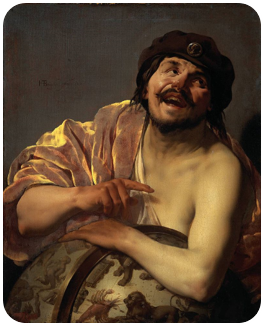
\includegraphics[width=3cm]{DEMOCRITUS}
			\captionof{figure}{Democritus (460 - 370,Hy Lạp)\label{fig:Democritus} }
		\end{center}
	\end{minipage}
	
	\begin{center}
		\includegraphics[width=12cm]{Historyatom}
		\captionof{figure}{Lịch sử phát triển mô hình nguyên tử \label{fig:Historyatom} }
	\end{center}
\end{hoplythuyet}
\subsubsection{Thành phần và cấu trúc của nguyên tử}
\paragraph{Thành phần}
\begin{hoplythuyet}
	Nguyên tử gồm hạt nhân chứa proton, neutron và vỏ nguyên tử chứa electron.
	\begin{center}
		\includegraphics[width=9cm]{mohinhnguyentu}
		\captionof{figure}{Mô hình nguyên tử}
	\end{center}
\end{hoplythuyet}
\paragraph{Sự tìm ra electron}
\ntd{Thí nghiệm khám phá tia âm cực của Thomson}\\
Năm 1897, J. J. Thomson (Tôm-xơn, người Anh) thực hiện thí nghiệm phóng điện qua không khí loãng đã phát hiện ra chùm tia phát ra từ cực âm.(xem hình \ref{fig:hinh3} ) và link video bằng mã QR ở bên dưới.\\ 
\hinhphai{\begin{center}
		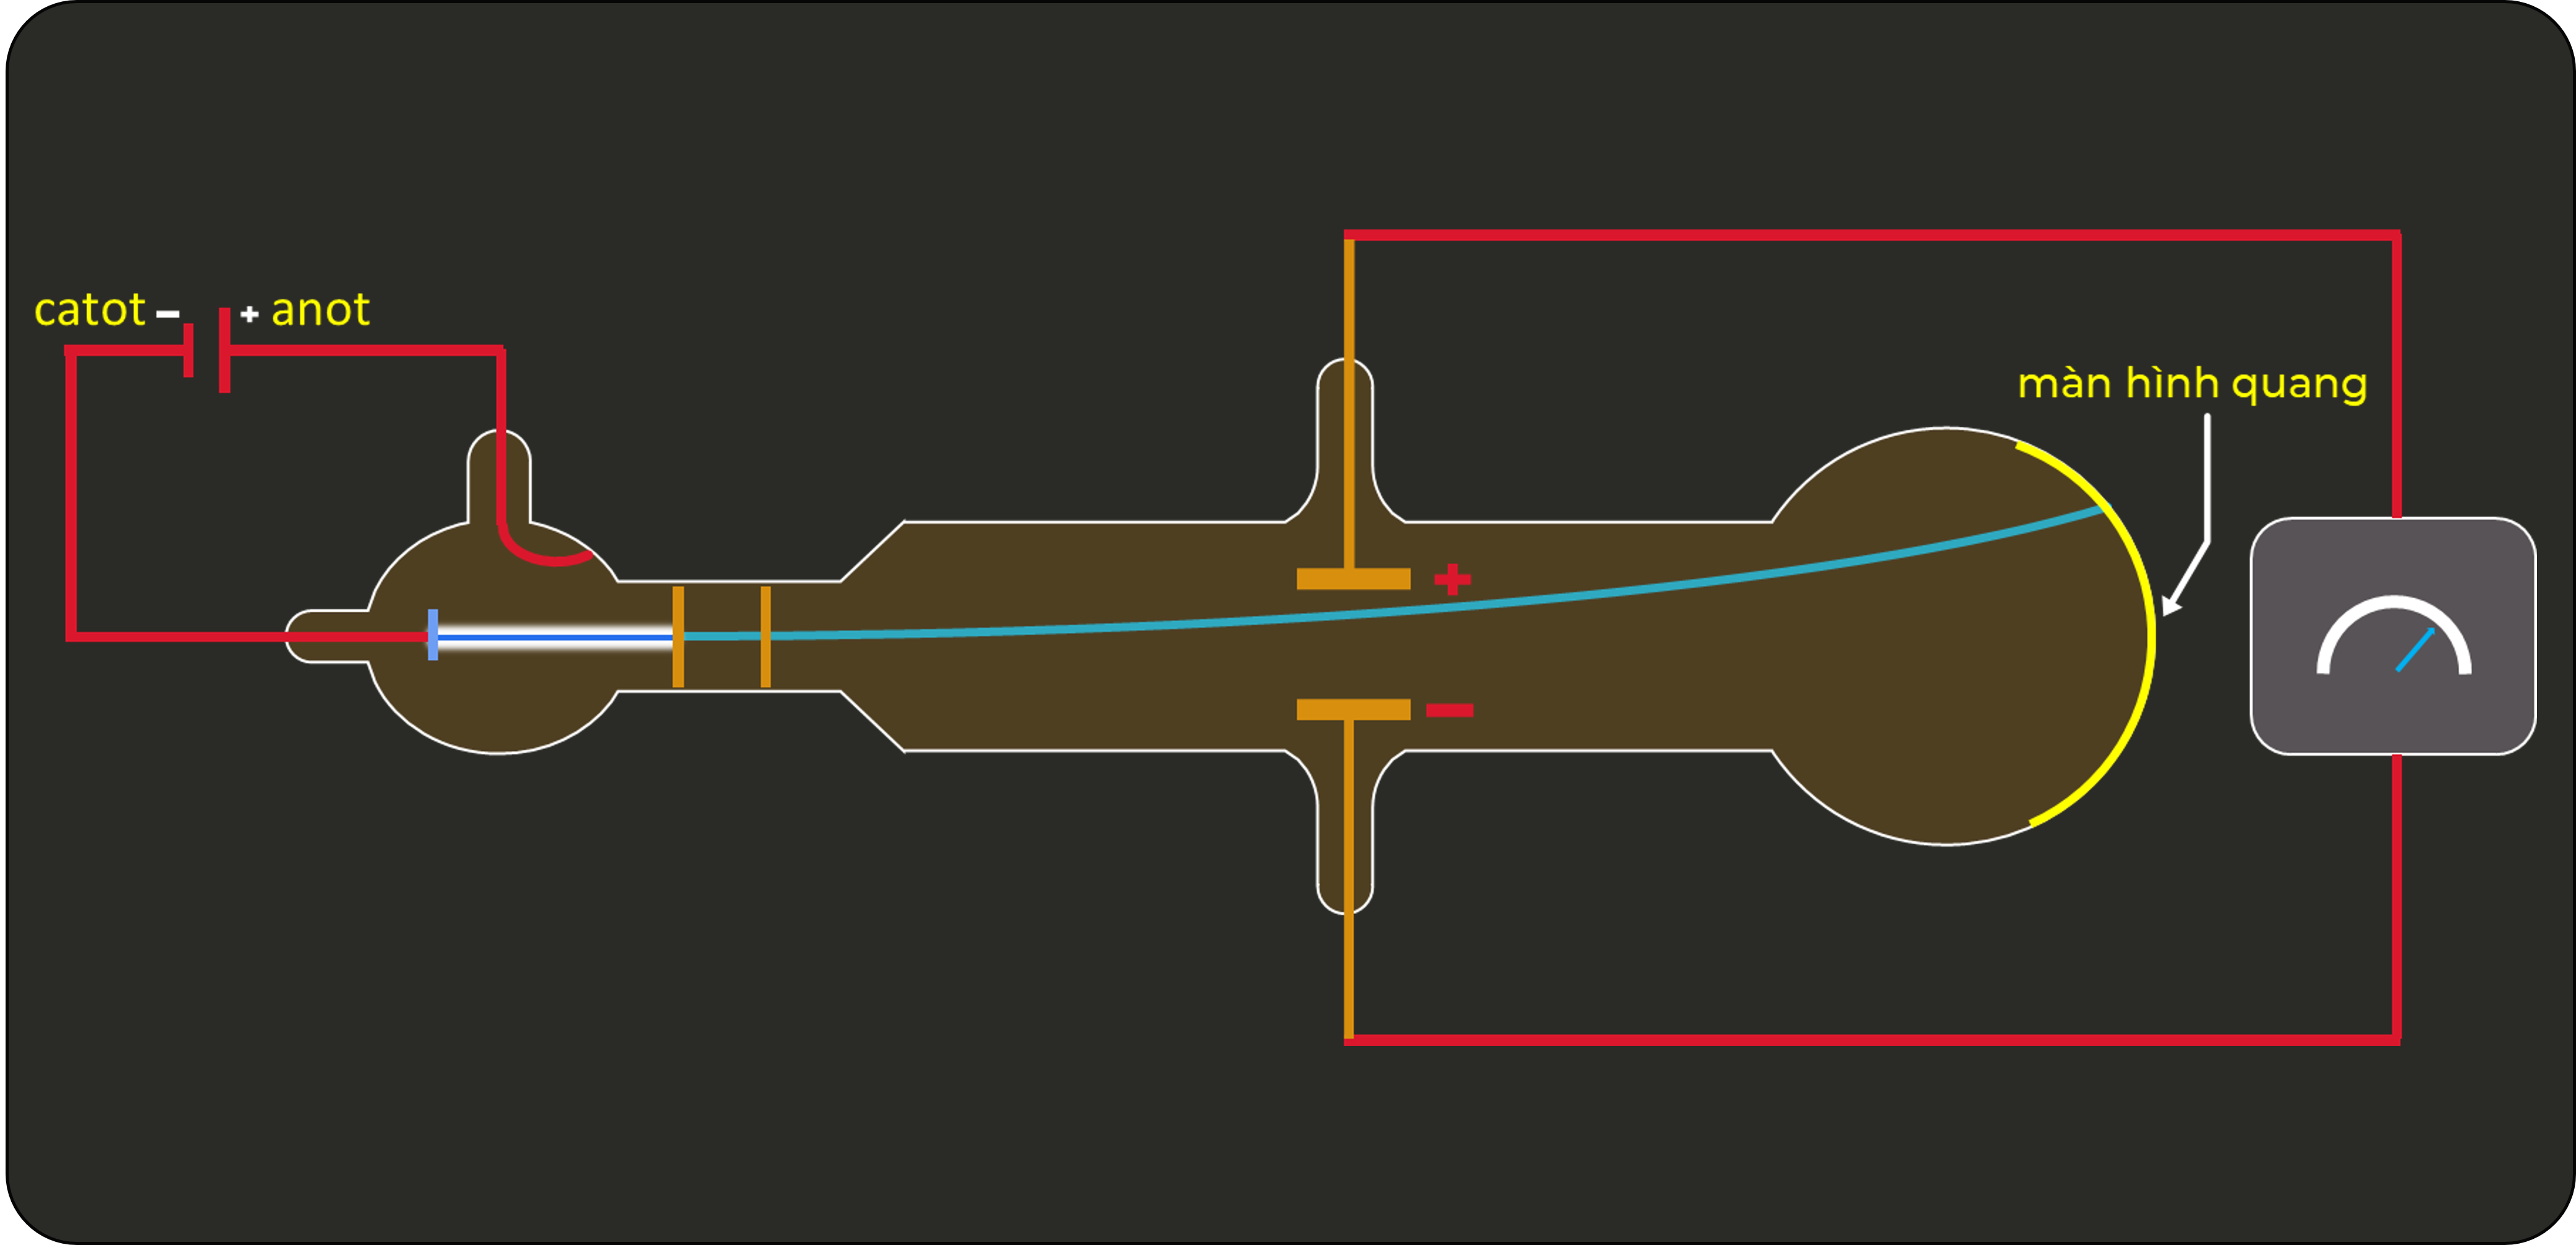
\includegraphics[width=9cm]{TNTHOMSON}\\
		\captionof{figure}{Thí nghiệm của Thomson}
		\label{fig:hinh3}
\end{center}}{\begin{tikzpicture}
		\path (0,0)  node (QRCODE) {\qrcode[height=2.0cm]{https://youtu.be/y2uswXtC5O8}}
		(QRCODE.south) node[anchor=north]{(\fmmfamily Các bạn  dùng ~\rotatebox{-15}{\faMobile}~quét mã QR để xem video TN nhé!)}
		;
\end{tikzpicture}}






\begin{hoivadap}
	Vai trò của lớp bột huỳnh quang trong thí nghiệm ở hình \ref{fig:hinh3}
	\huongdan{\taodongke{10}}
\end{hoivadap}

\begin{hoivadap}
	Quan sát Hình \ref{fig:hinh3} và video , giải thích vì sao tia âm cực bị hút về cực dương của trường điện.
	\huongdan{\taodongke{10}}
\end{hoivadap}

\begin{hoivadap}
	Nếu đặt một chong chóng nhẹ trên đường đi của tia âm cực thì chong chóng sẽ quay. Từ hiện tượng đó, hãy nêu kết luận về tính chất của tia âm cực.
	\huongdan{\taodongke{5}}
\end{hoivadap}
\newpage
\vspace*{6pt}
\begin{emcobiet}
	Mô hình Thomson còn gọi là mô hình \lq\lq bánh pudding mận".Theo Thomson:
	\begin{enumerate}
		\item Nguyên tử là quả cầu mang điện tích dương, bên trong chứa các êlectron.
		\item Nguyên tử trung hòa về điện.
	\end{enumerate}
	
\end{emcobiet}


\paragraph{Sự khám phá hạt nhân nguyên tử}
\ntd{Tìm hiểu thí nghiệm của Rutherford}\\
Năm 1911, E. Rutherford (Ro-dơ-pho, người Niu Di-lân) thực hiện thí nghiệm bắn phá lá vàng rất mỏng bằng chùm hạt $ \alpha $ \footnote{Hạt $\alpha$ : hạt nhân helium, mang điện tích dương.} (xem hình \ref{fig:hinh4})
\begin{center}
	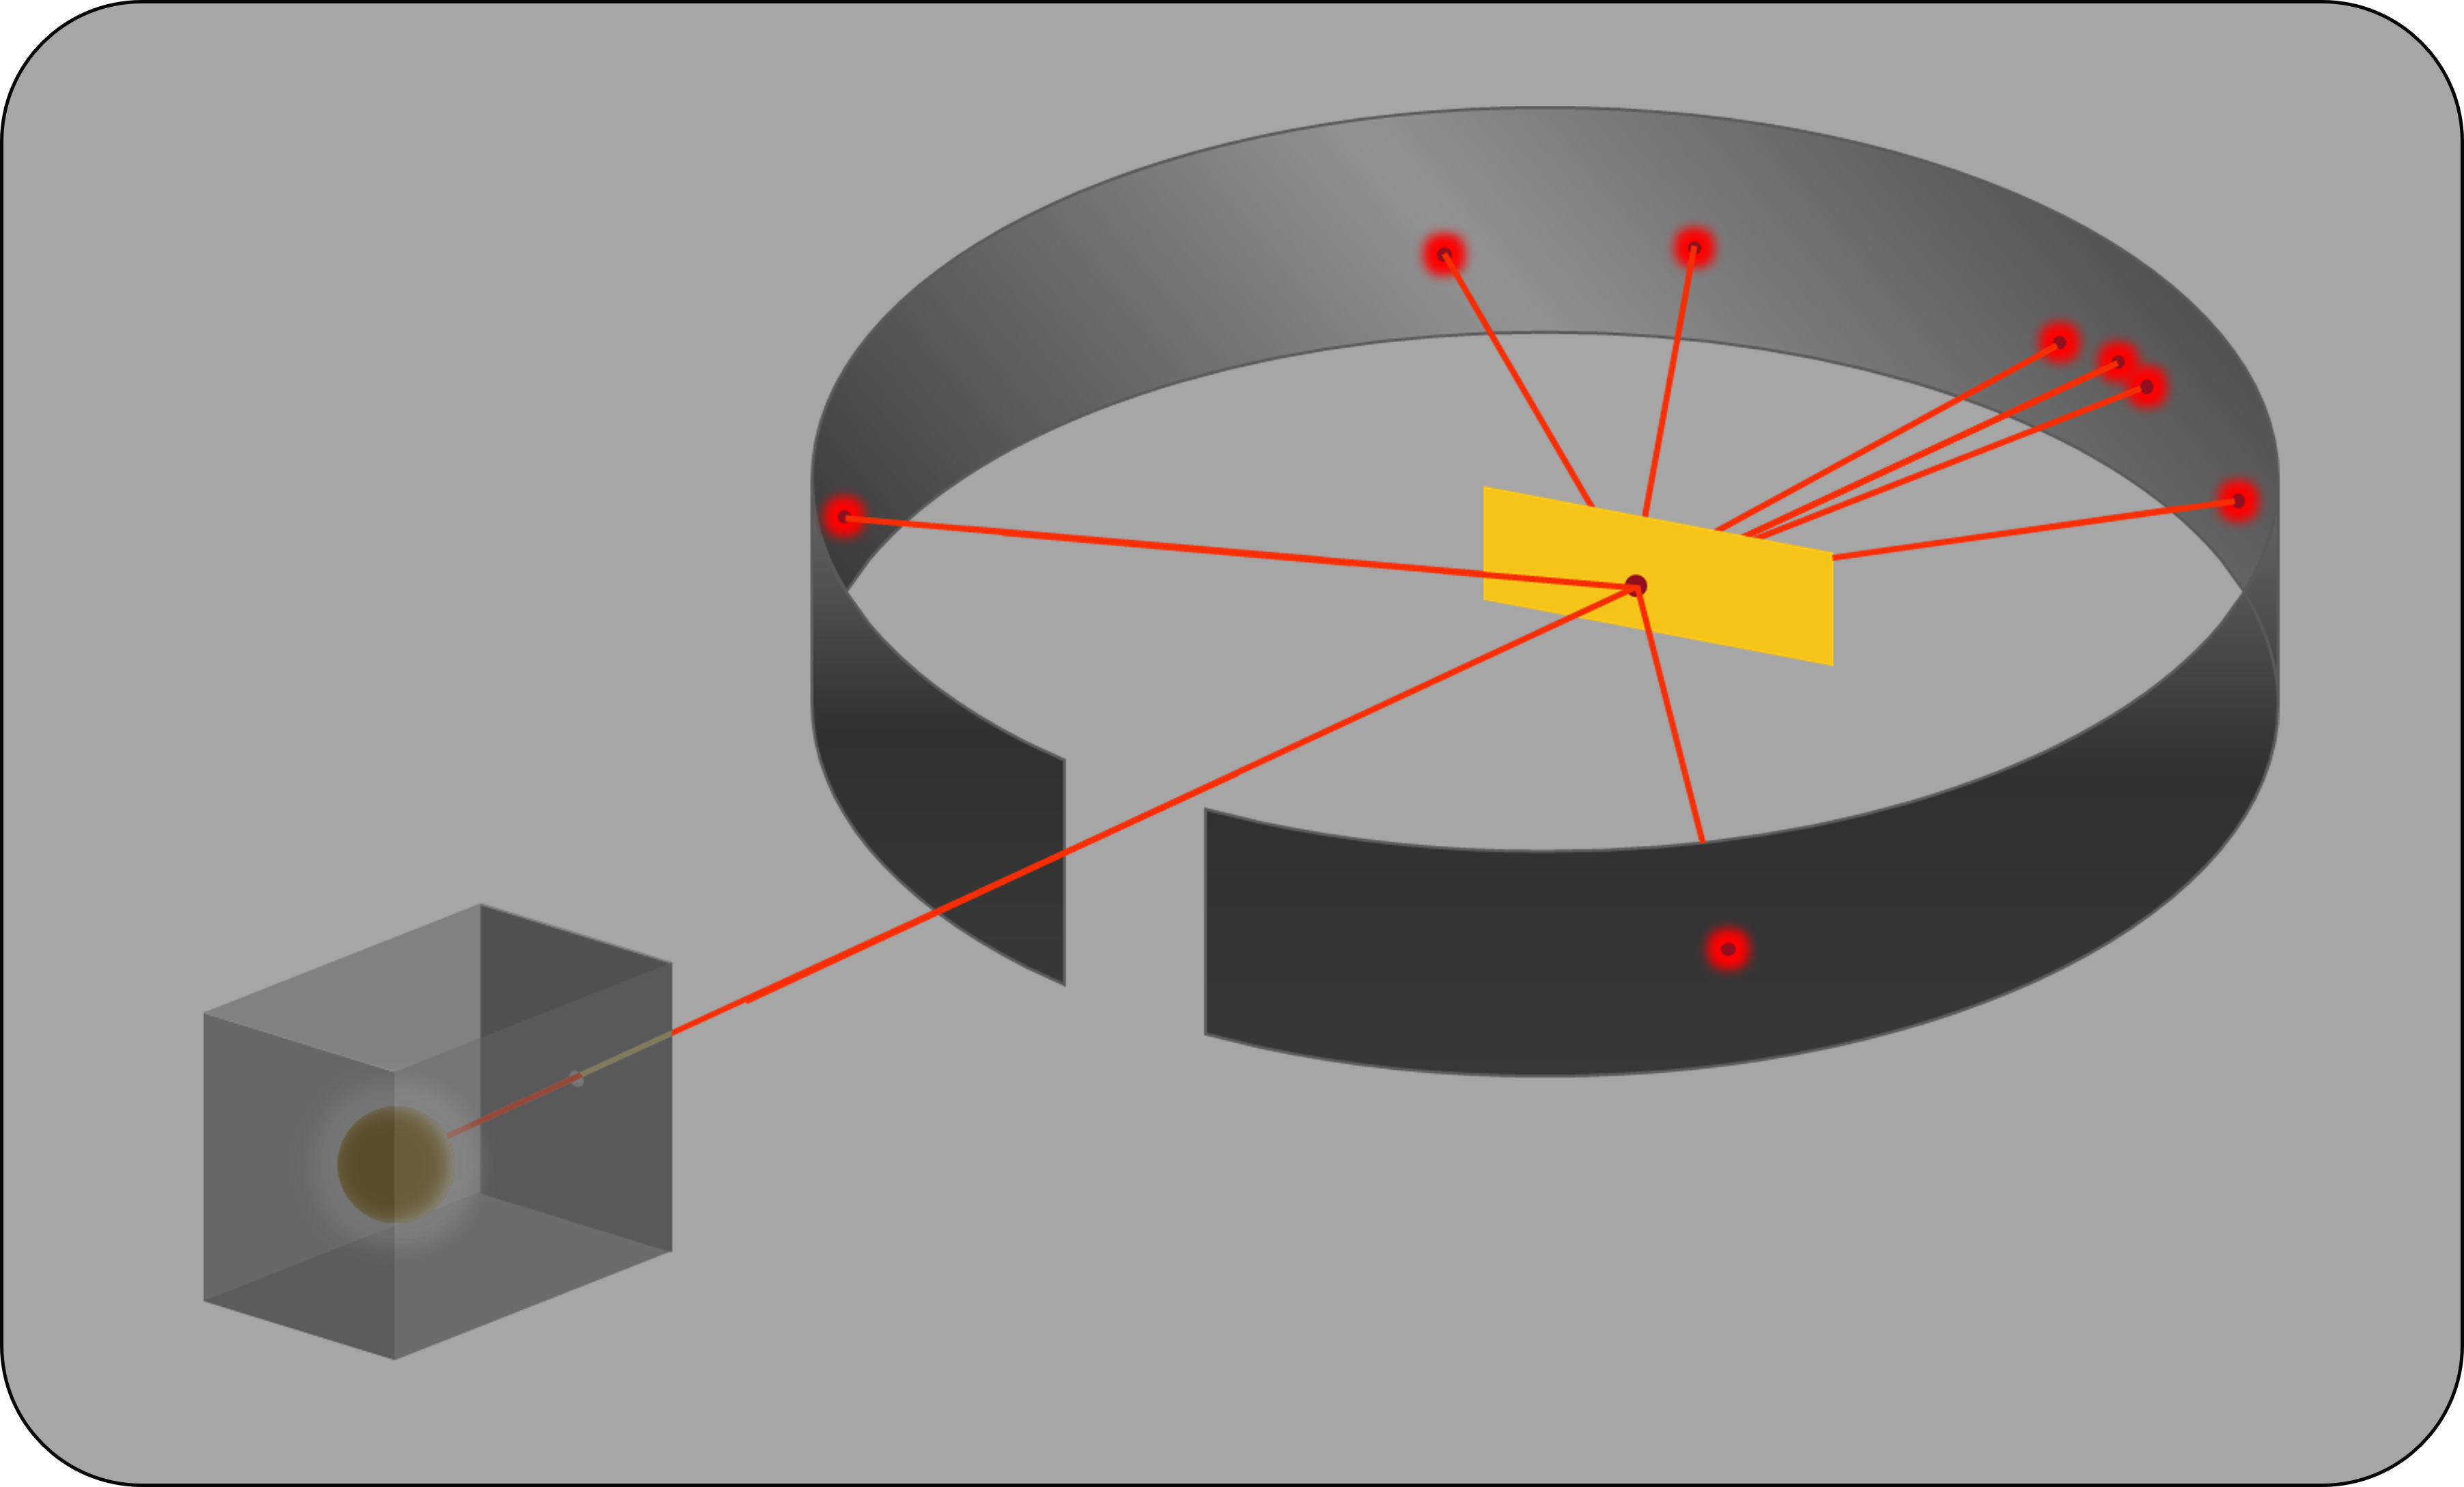
\includegraphics[width=9cm]{TNRUTHERFORT}\\
	\captionof{figure}{Thí nghiệm của Rutherford}
	\label{fig:hinh4}
\end{center}

\begin{center}
	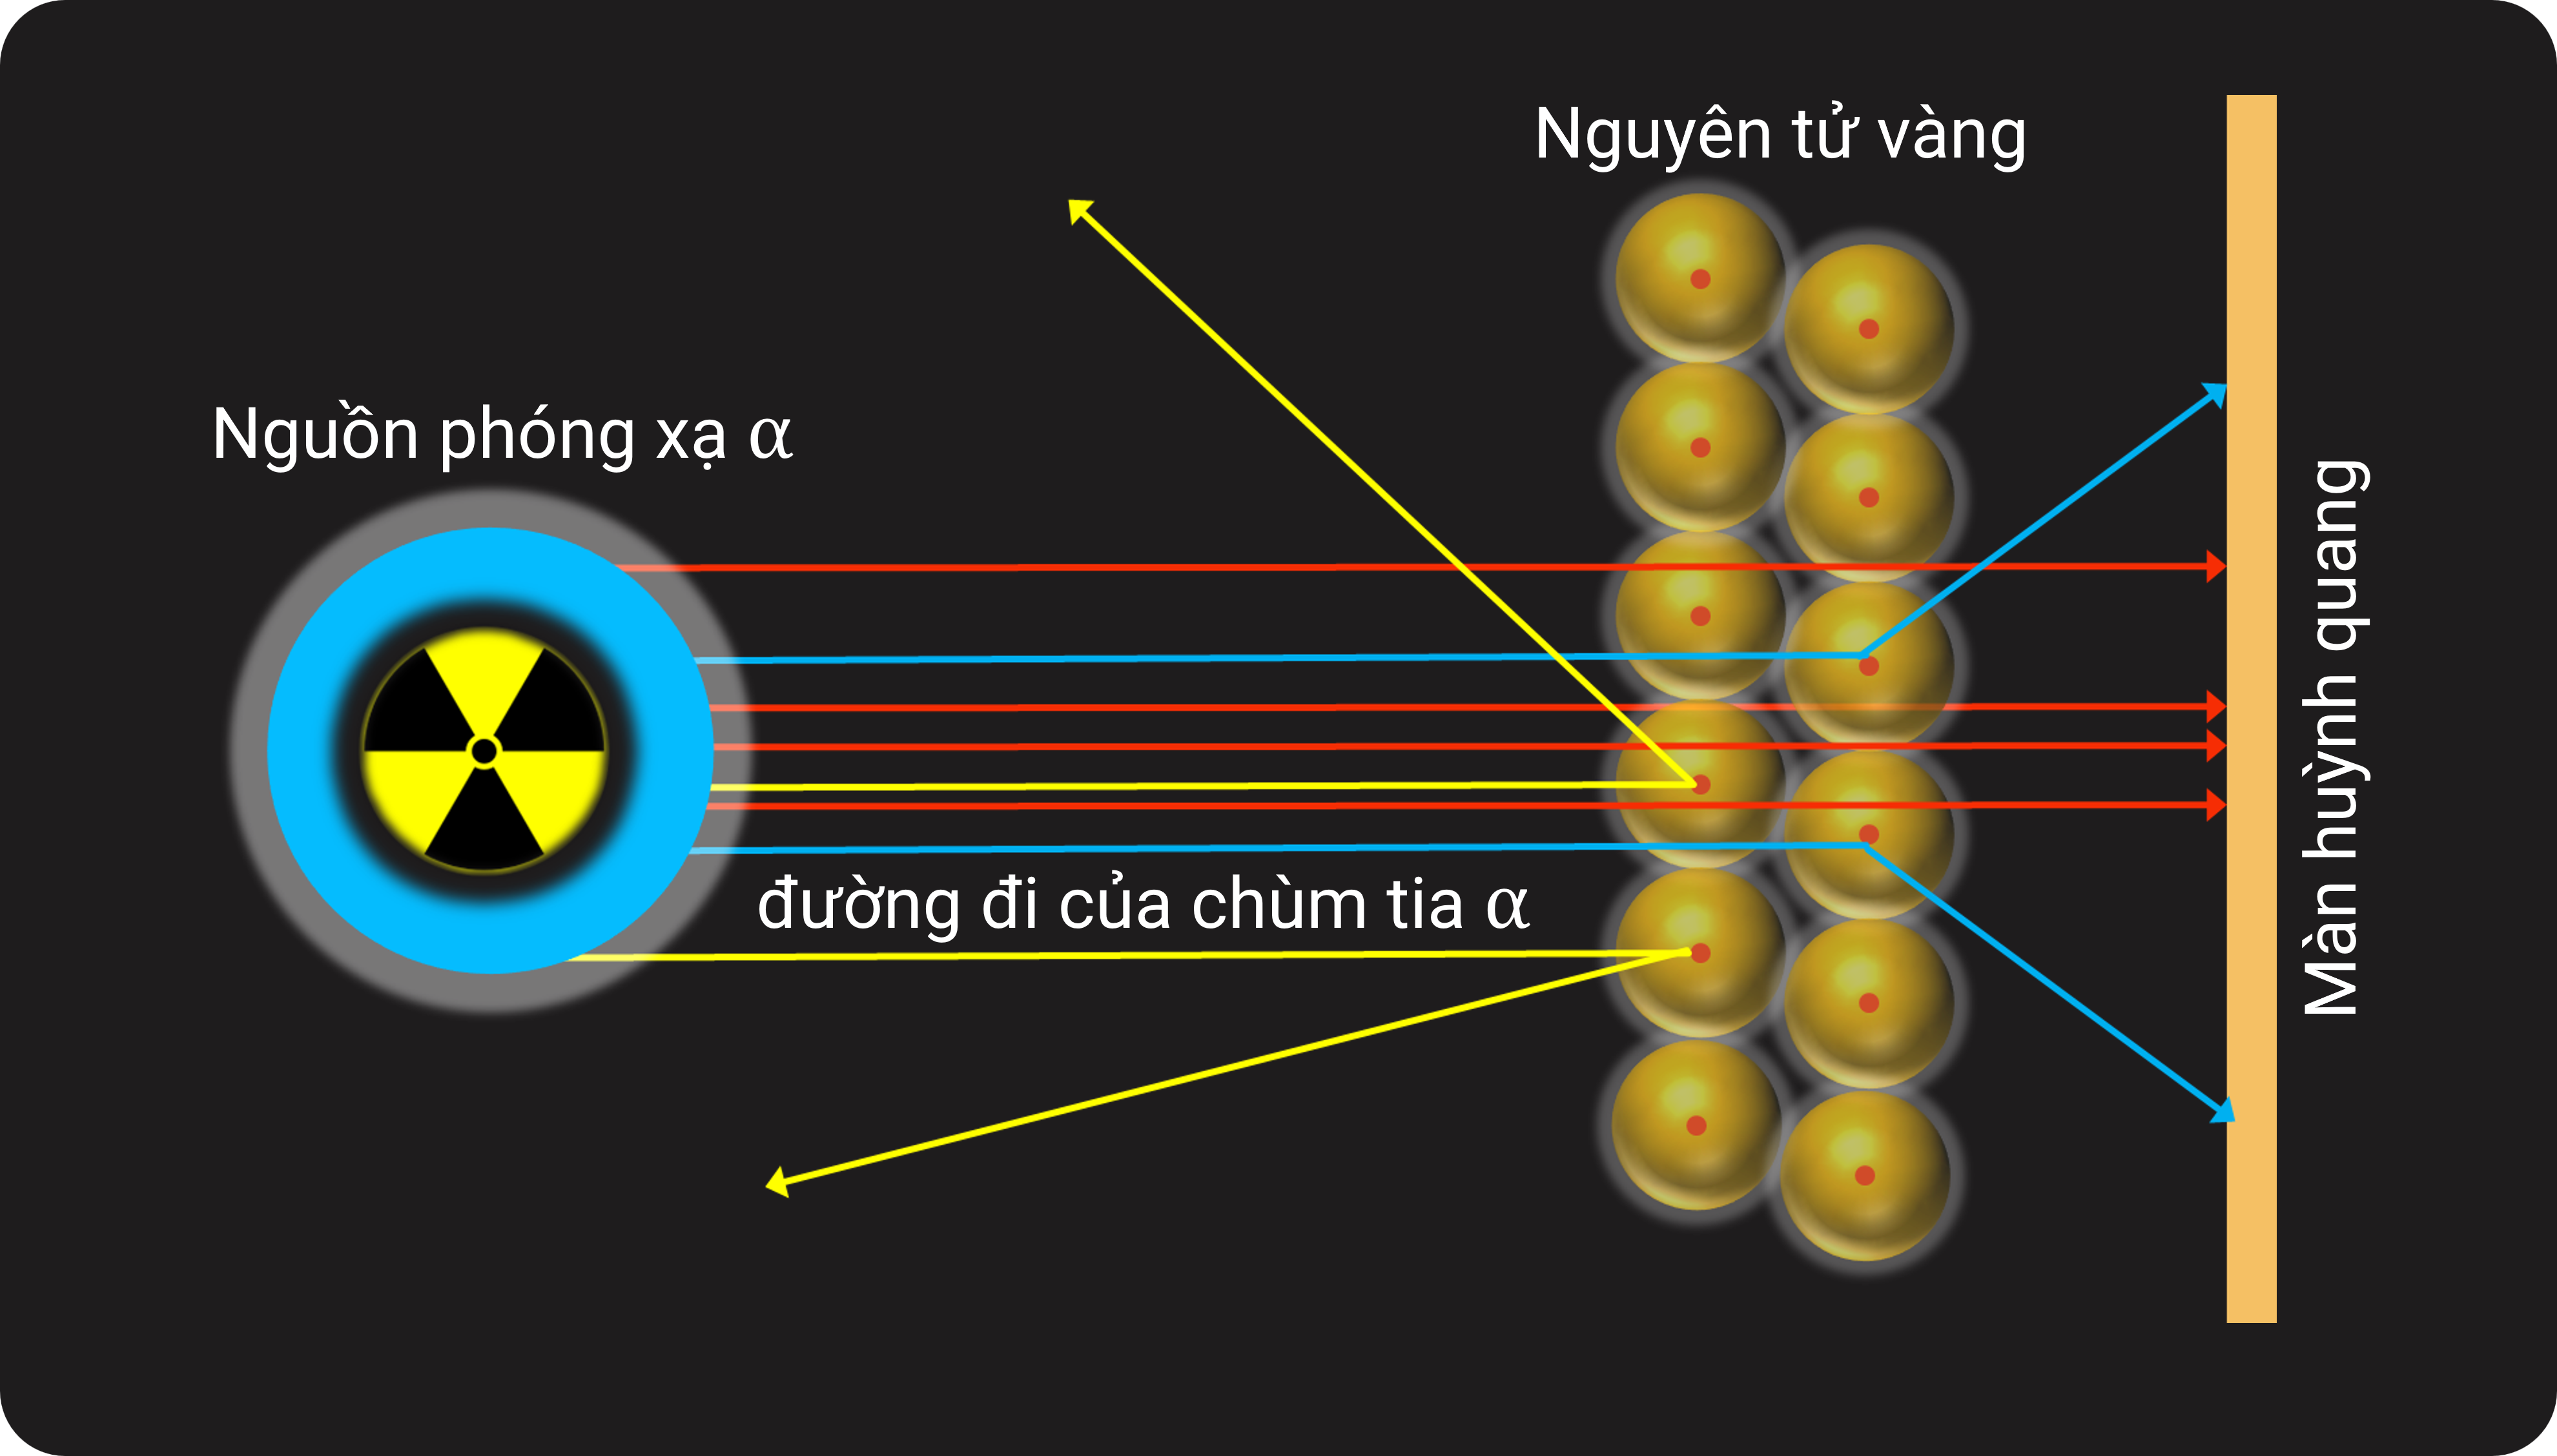
\includegraphics[width=9cm]{KQTN}\\
	\captionof{figure}{Kết quả thí nghiệm của Rutherford}
	\label{fig:hinh5}
\end{center}

\begin{hoivadap}
	Quan sát hình \ref{fig:hinh4}, cho biết các hạt $\alpha$ có đường đi như thế nào. Dựa vào Hình \ref{fig:hinh5} , giải thich kết quả thí nghiệm thu được.
	\huongdan{\taodongke{5}}
\end{hoivadap}
\vspace*{6pt}
\begin{hoplythuyet}
	{\bfseries{Kết luận}}
	\begin{itemize}
		\item Nguyên tử có cấu tạo rỗng, gồm hạt nhân ở trung tâm và lớp vỏ là các electron chuyển động xung quanh hạt nhân.
		\item Nguyên tử trung hoà về điện: số đơn vị điện tích dương của hạt nhân bằng số đơn vị điện tích âm của các electron trong nguyên tử.
	\end{itemize}
\end{hoplythuyet}
\paragraph{Cấu tạo hạt nhân nguyên tử}
\begin{center}
	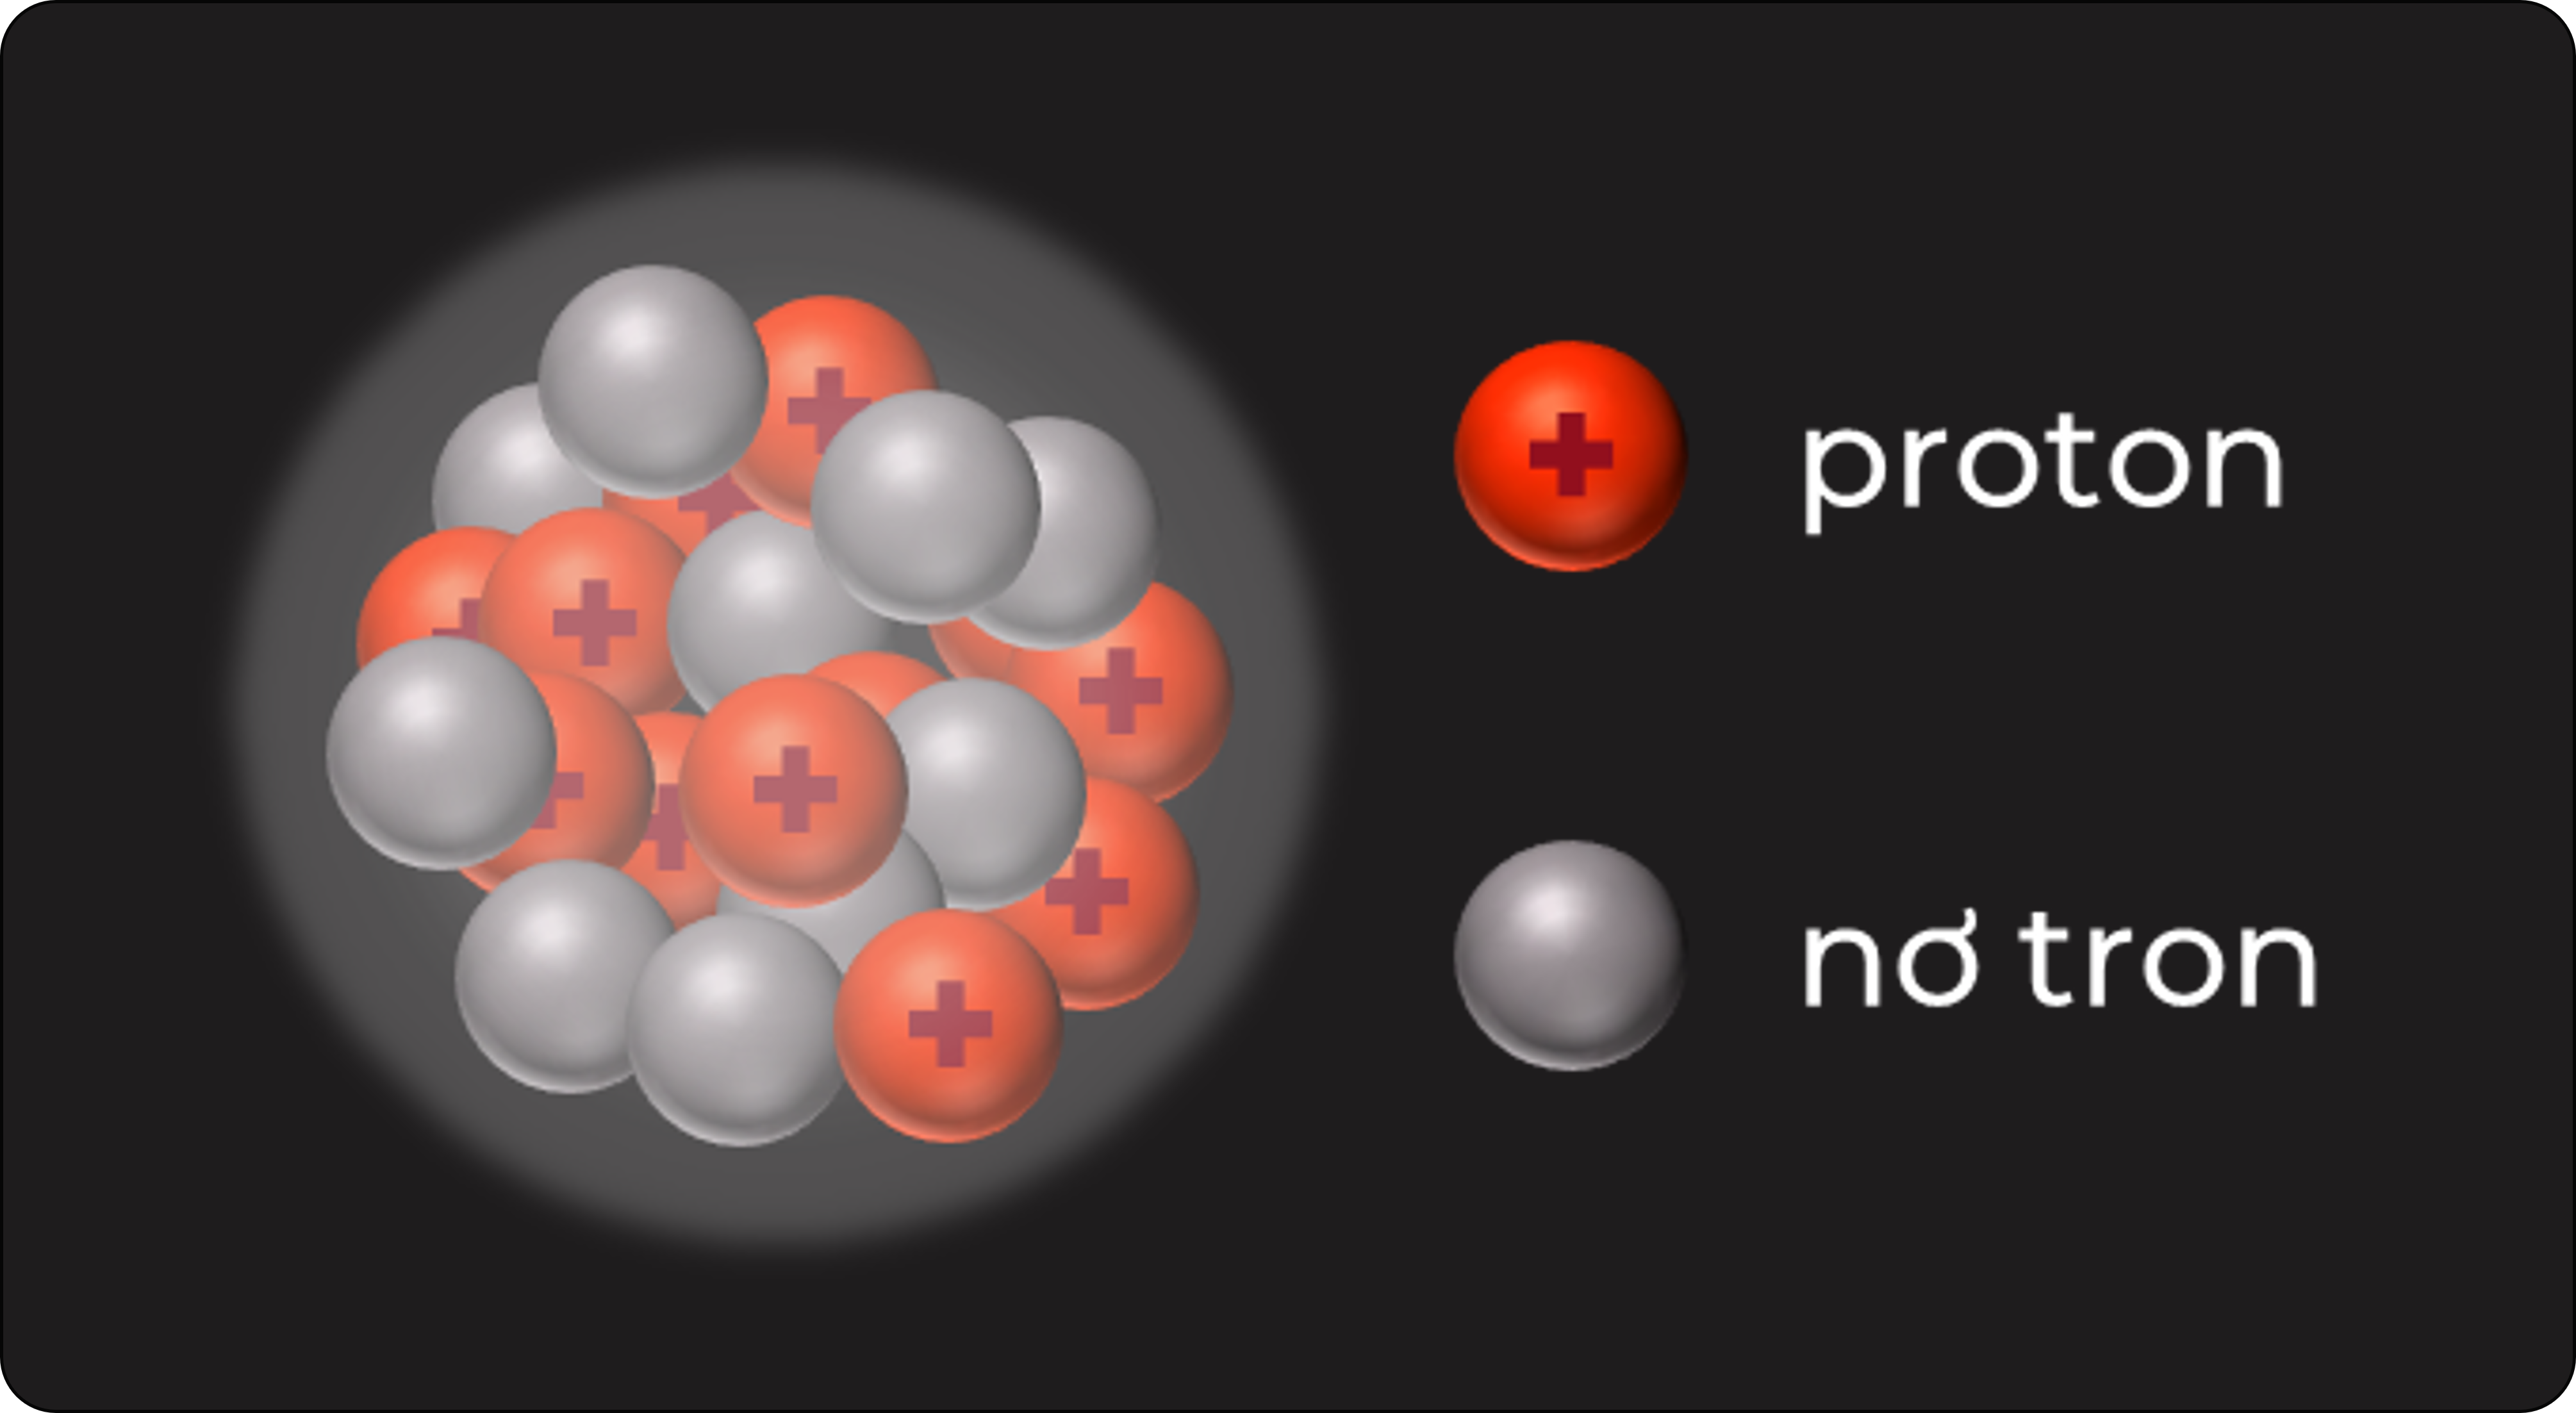
\includegraphics[width=9cm]{CAUTAOHATNHAN}\\
	\captionof{figure}{Thành phần của hạt nhân}
	\label{fig:hinh6}
\end{center}
\begin{hoivadap}
	Quan sát hình \ref{fig:hinh6} và kết hợp SGK , các bạn hãy nêu thành phần của hạt nhân
\end{hoivadap}
\begin{hoplythuyet}
	Proton, neutron và electron là các hạt cấu tạo nên nguyên tử.
\end{hoplythuyet}
\begin{tongket}
	Thành phần cấu tạo của nguyên tử gồm:
	\begin{itemize}
		\item  Hạt nhân (nucleus): ở tâm của nguyên tử, chứa các proton mang điện tích dương và các neutron không mang điện.
		\item Vỏ nguyên tử: chứa các electron mang điện tích âm, chuyển động rất nhanh xung quanh hạt nhân.
		\item Trong nguyên tử, số proton bằng số electron nên nguyên tử trung hoà điện.
		\item Khối lượng của electron rất nhỏ, không đáng kể so với khối lượng của proton hay neutron nên khối lượng của nguyên tử tập trung hầu hết ở hạt nhân.
	\end{itemize}
\end{tongket}


\begin{longtable}{|c|c|c|c|c|c|}
	\caption{\indam[dndo]{Khối lượng, điện tích của các loại hạt cấu tạo nên nguyên tử}}
	\label{tab:table1}\\
	\hline
	\rowcolor{dnxanh!25} \indam[dnxanh]{Hạt} & \indam[dnxanh]{Kí hiệu} & $\begin{array}{c}\text {\indam[dnxanh]{Khối lượng} } \\
		\text {\indam[dnxanh]{(kg)}  }\end{array}$ & \indam[dnxanh]{Khối lượng (amu)} & $\begin{array}{c}\text { \indam[dnxanh]{Điện tích} } \\
		\text { \indam[dnxanh]{(C)} }\end{array}$ & $\begin{array}{l}\text { \indam[dnxanh]{Điện tích} } \\
		\text { \indam[dnxanh]{tương đối} }\end{array}$ \\
	\hline\endhead
	\rowcolor{dnvang!15} Proton & $p$ & $1,672 \cdot 10^{-27}$ & $\approx 1$ & $1,602 \cdot 10^{-19}$ & +1 \\
	\hline
	\rowcolor{dnvang!15} Neutron & $\mathrm{n}$ & $1,675 \cdot 10^{-27}$ & $\approx 1$ & 0 & 0 \\
	\hline\rowcolor{dnvang!15} Electron & e & $9,109 \cdot 10^{-31}$ & $\begin{array}{c}
		~ \\
		\dfrac{1}{1837} \approx 0,00055\\
		~ \\
	\end{array}$ & $-1,602 \cdot 10^{-19}$ & -1 \\
	\hline
\end{longtable}
\paragraph{KíCH THƯỚC VÀ KHỐI LƯợNG NGUYÊN TỬ}
\begin{center}
	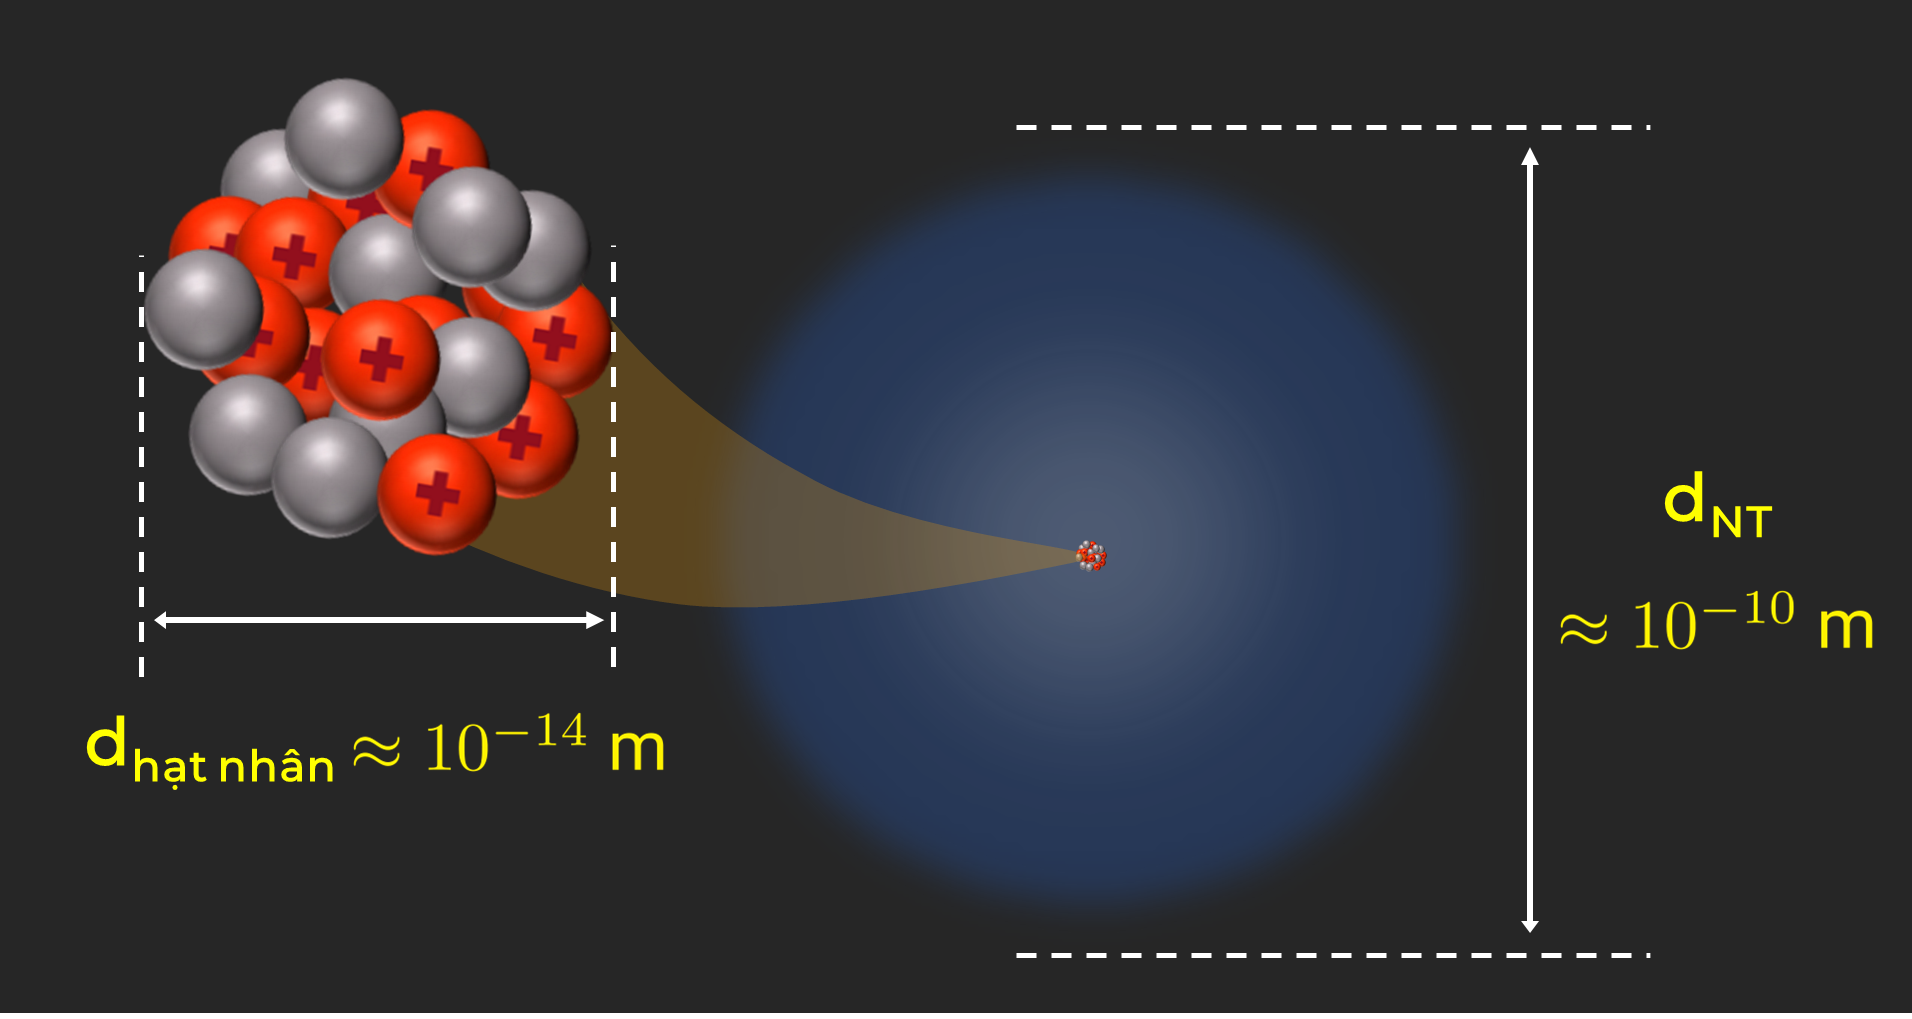
\includegraphics[width=9cm]{ktnt}\\
	\captionof{figure}{So sánh kích thước hạt nhân , nguyên tử}
	\label{fig:hinh7}
\end{center}
\begin{notegsnd}
	\begin{itemize}
		\item Đơn vị kích thước thường dùng của nguyên tử là Angstron ($ A^0 $) hoặc nano mét (nm)			
		$$1 \mathrm{~nm}=10^{-9}~\mathrm{m} ; 1 A^0=10^{-10}~\mathrm{~m} ; 1 \mathrm{~nm}=10 A^0; 1 A^0=10^{2}~\mathrm{pm}$$
		\begin{center}
			\tcbox[width=5cm,colframe=dndo]{$ \dfrac{d_{\text{NT}}}{d_{\text{hạt nhân}}}\approx \dfrac{10^{-10}}{10^{-14}} \approx 10^4~\mathrm{\text{lần}} $}
		\end{center}
		\item Đơn vị của khối lương nguyên tử là amu (atomic mass unit),
		$$
		1 \mathrm{amu}=1,6605 \times 10^{-27} \mathrm{~kg} \text {. }
		$$
		\item Đơn vi của điện tích các hạt cơ bản là $\mathrm{e}_0$ (điện tích nguyên tố),
		$$
		1 \mathrm{e}_0=1,602 \times 10^{-19} \mathrm{C} \text {. }
		$$
	\end{itemize}
\end{notegsnd}
\newpage
\vspace*{3pt}

\ntd{BÀI TẬP TRẮC NGHIỆM}:
\begin{dangntd}{LÝ THUYẾT VỀ CẤU TẠO NGUYÊN TỬ}
	\giaibaitap{Phương pháp giải}
	\begin{itemize}
		\item Nắm vững về cấu tạo nguyên tử
		\item Nắm vững kết quả thí nghiệm của Thomson,Rutherford
	\end{itemize}
\end{dangntd}
\Opensolutionfile{ansbook}[DAPAN/BTTLH10CO102tachLG]
\Opensolutionfile{ans}[DAPAN/BTTLH10CO102]
\begin{ex}[1]
	Các hạt cơ bản của hầu hết các nguyên tử là?
	\choice
	{%
		electron
	}
	{%
		electron và proton
	}
	{%
		proton và notron
	}
	{%
		\True electron, proton và notron
	}
	\sodongkeex[5]
\end{ex}


\begin{ex}[1]
	Hạt nhân của hầu hết các nguyên tử gồm có?
	\choice
	{%
		electron
	}
	{%
		electron và proton
	}
	{%
		\True proton và notron
	}
	{%
		electron, proton và notron
	}
	\sodongkeex[5]
\end{ex}

\begin{ex}[2]
	Trong thí nghiệm của Thomson, phát biểu nào sau đây sai với kết quả thí nghiệm ta quan sát được?
	\choice
	{%
		Tia âm cực là các chùm hạt electron di chuyển từ cực âm sang cực dương
	}
	{%
		Tia âm cực là chùm hạt mang điện tích âm
	}
	{%
		\True	Tia âm cực bị lệch về phía bản cực âm của nguồn điện
	}
	{%
		Tia âm cực bị lệch hướng khi ta đặt nó trong từ trường
	}
	\sodongkeex[5]
\end{ex}

\begin{ex}[2]
	Theo mô hình bánh pudding mận của Thomson, phát biểu nào sau đây là đúng?
	\choice
	{%
		Nguyên tử có cấu tạo rỗng gồm hạt nhân mang điện tích dương và vỏ là các electron chuyển động xung quanh hạt nhân.
	}
	{%
		Nguyên tử có cấu tạo rỗng gồm hạt nhân mang điện tích dương và vỏ là các electron chuyển dộng xung quanh hạt nhân theo những quỹ đạo có kích thước và năng lượng cố định
	}
	{%
		\True	nguyên tử bao gồm các electron nằm rải rác trong một đám mây hình cầu mang điện tích dương.
	}
	{%
		các electron  quay quanh hạt nhân không theo một quỹ đạo xác định, mà chúng tạo thành các đám mây điện tích mà tại đó xác suất tìm thấy electron là lớn nhất
	}
	\sodongkeex[5]
\end{ex}
\begin{ex}[2]
	Cho các phát biểu sau:
	\begin{enumerate}[(1)]
		\item Tất cả các hạt nhân nguyên tử đều được cấu tạo từ các hạt proton và neutron.
		\item Khối lượng nguyên tử tập trung phần lớn ở lớp vỏ.
		\item Trong nguyên tử, số electron bằng số proton.
		\item Trong hạt nhân nguyên tử, hạt mang điện là proton và electron.
		\item Trong nguyên tử, hạt electron có khối lượng không đáng kể so với các hạt còn lại.
	\end{enumerate}
	Số phát biểu đúng là
	\choice
	{%
		1
	}
	{%
		\True 2
	}
	{%
		3
	}
	{%
		4
	}
	\huongdan{%
		Phát biểu đúng là:
		Trong hạt nhân nguyên tử, hạt mang điện là proton và electron.\\
		Trong nguyên tử, hạt electron có khối lượng không đáng kể so với các hạt còn lại
	}
	
\end{ex}

\begin{ex}[2]
	Điều nào sau đây đúng theo mô hình nguyên tử của Thomson?
	\choice
	{%
		Nguyên tử không trung hòa về điện
	}
	{%
		\True Nguyên tử là quả cầu mang điện tích dương có chứa các êlectron bên trong
	}
	{%
		Điện tích âm và điện tích dương trong nguyên tử có độ lớn bằng nhau
	}
	{%
		Không có điều nào ở trên
	}
	\sodongkeex[5]
\end{ex}


\begin{ex}[3]
	Trong hiện tượng xả điện qua khí ở áp suất thấp, sự tỏa sáng màu trong ống xuất hiện là kết quả của:
	\choice
	{% 
		\True va chạm giữa các hạt mang điện được phát ra từ cực âm và nguyên tử của khí
	}
	{% 
		va chạm giữa các electron khác nhau của các nguyên tử trong khí
	}
	{% 
		kích thích các electron trong các nguyên tử
	}	
	{% 
		va chạm giữa các nguyên tử của khí
	}	
	\sodongkeex[5]	
\end{ex}

\begin{ex}[2]
	Mô hình đầu tiên về nguyên tử được đưa ra bởi:
	\choice
	{%
		N. Bohr
	}
	{% 
		E. Goldstein
	}
	{% 
		Rutherford
	}
	{% 	
		\True J.J. Thomson
	}
	\sodongkeex[5]
\end{ex}

\begin{ex}[2]
	Nếu đường kính của nguyên tử khoảng $10^2 \mathrm{pm}$ thì đường kính của hạt nhân khoảng
	\choice
	{%
		$10^2 \mathrm{pm}$
	}
	{%
		$10^{-4} \mathrm{pm}$
	}
	{%
		\True	$10^{-2} \mathrm{pm}$
	}
	{
		$10^4 \mathrm{pm}$
	}
	\sodongkeex[5]
\end{ex}
\Closesolutionfile{ans}
\Closesolutionfile{ansbook}


\newpage
\giaibaitap{BÀI TẬP TỰ LUẬN}
\Opensolutionfile{ansbt}[DAPAN/BT_H10C0102]
\begin{btex}[2]
	Trong thí nghiệm của Rutherford, khi sử dụng các hạt alpha (ion $\mathrm{He}^{2+}$, kí hiệu là $\mathrm{a}$ ) bắn vào lá vàng thì:
	\begin{itemize}
		\item Hầu hết các hạt a xuyên thẳng qua lá vàng.
		\item Một số ít hạt a bị lệch quỹ đạo so với ban đầu.
		\item Một số rất ít hạt a bị bật ngược trở lại.
	\end{itemize}
	Từ kết quả này, em có nhận xét gì về cấu tạo nguyên tử?
	\loigiai{
		Trong thí nghiệm của Rutherford, khi sử dụng các hạt alpha (ion $\mathrm{He}^{2+}$, kí hiệu là a) bắn vào lá vàng thì:
		\begin{itemize}
			\item Hầu hết các hạt a xuyên thẳng qua lá vàng chứng tỏ nguyên tử có cấu tạo rỗng.
			\item Một số ít hạt a bị lệch quỹ đạo so với ban đầu chứng tỏ hạt nhân nguyên tử cùng điện tích dương như hạt hạt alpha (ion $\mathrm{He}^{2+}$, kí hiệu là $ \alpha $).
			\item Một số rất ít hạt a bị bật ngược trở lại chứng tỏ kích thước hạt nhân nhỏ hơn rất nhiều so với kích thước của nguyên tử và khối lượng nguyên tử tập trung chủ yếu ở hạt nhân.
		\end{itemize}
		
	}
\end{btex}

\begin{btex}[2]
	Viết lại bảng sau vào vở và điền thông tin còn thiếu vào các ô trống:\\
	\begin{tabular}{|c|c|c|c|c|c|c|}
		\rowcolor{dnxanh!25} 
		\hline \indam[dnxanhdam]{Nguyên tố} & \indam[dnxanhdam]{Kí hiệu} & \color{dnxanhdam} {$\mathbf{Z}$} & \indam[dnxanhdam]{Số e} & \indam[dnxanhdam]{Số p} & \indam[dnxanhdam]{Số n} & \indam[dnxanhdam]{Số khối} \\
		\rowcolor{dnvang!25} 
		\hline \indam[dnxanhdam]{Carbon} & $\mathrm{C}$ & 6 & 6 & $?$ & 6 & $?$ \\
		\rowcolor{dnvang!25} 
		\hline \indam[dnxanhdam]{Nitrogen} & $\mathrm{N}$ & 7 & $?$ & 7 & $?$ & 14 \\
		\rowcolor{dnvang!25} 
		\hline \indam[dnxanhdam]{Oxygen} & $\mathrm{O}$ & 8 & 8 & $?$ & 8 & $?$ \\
		\rowcolor{dnvang!25} 
		\hline \indam[dnxanhdam]{Sodium (natri)} & $\mathrm{Na}$ & 11 & $?$ & 11 & $?$ & 23 \\
		\rowcolor{dnvang!25}
		\hline \indam[dnxanhdam]{Aluminium (nhôm)} & $\mathrm{Al}$ & $?$ & 13 & $?$ & $?$ & 27 \\
		\hline
	\end{tabular}
	\huongdan{
		\taodongke{5}
	}
\end{btex}

\Closesolutionfile{ansbt}










\newpage
\begin{dangntd}{Bài tập về khối lượng, kích thước nguyên tử}	
	\giaibaitap{Phương pháp giải}\\
	\tieumuc{Các công thức liên quan khối lượng}
	\begin{itemize}
		\item $ m _{\text{nguyên tử}=m_{p}+m_{n} + m_{e} } $ (tính chính xác); $ m _{\text{nguyên tử}} \approx  m_{p} + m_{n} \approx m_{\text{hạt nhân}} $ (tính gần đúng)
		\item Khối lượng tính ra kg của 1 nguyên tử carbon-12 là $ 19,926 . 10^{27}~\mathrm{kg}$.
		\item 1 amu được định nghĩa bằng $\dfrac{1}{12}$ khối lượng 1 nguyên tử carbon-12:
		\item$1 \mathrm{amu}=\dfrac{19,926 \cdot 10^{-27} \mathrm{~kg}}{12}=1,661 \cdot 10^{-27} \mathrm{~kg}$
		\item$1 \mathrm{mol}$ chứa $ 6,02.10^{23} $ nguyên tử, phân tử, ion.
	\end{itemize}
	\tieumuc{Các công thức liên quan kích thước}
	\begin{itemize}
		\item Thể tích của hình cầu:
		$ V=\dfrac{4}{3}\pi r^3 $
		\item Phần trăm thể tích các nguyên tử trong tinh thể $ = \dfrac{V_{\text{các nguyên tử}}}{V_{\text{tinh thể}}}\cdot 100\% $
		\item Một số đơn vị đo: 
		$\left\{\begin{array}{l}
			1~\mathrm{nm} = 10^{-9}~\mathrm{m}\\
			1~\mathrm{A^{0}} = 10^{-10}~\mathrm{m}\\
			1~\mathrm{pm} = 10^{-12}~\mathrm{m}	
		\end{array}\right.$
	\end{itemize}
\end{dangntd}
\begin{vdm}{Ví dụ mẫu}
\end{vdm}

%Câu 1: Khối lượng của nguyên tử magnesium là $39,8271 \cdot 10^{-27} \mathrm{~kg}$. Khối lượng của magnesium theo amu là
%A. 23,978
%B. $66,133 \cdot 10^{-51}$.
%C. 24,000 .
%D. $23,985 \cdot 10^{-3}$.

\begin{vdex}[2]	
	Khối lượng của nguyên tử magnesium là $39,8271 \cdot 10^{-27} \mathrm{~kg}$. Khối lượng của magnesium theo amu là
	\choice
	{%
		\True $ 23,978 $
	}
	{%
		$66,133 \cdot 10^{-51}$
	}
	{%
		$23,985 \cdot 10^{-3}$
	}
	{%
		$ 24,000 $
	}
	\huongdan{
		
	}	
\end{vdex}

\begin{vdex}[2]
	Khối lượng tuyệt đối của một nguyên tử oxygen bằng $26,5595.10^{-27} \mathrm{~kg}$. Hãy tính khối lượng nguyên tử (theo amu) và khối lượng mol nguyên tử (theo g) của nguyên tử này.
	\loigiai
	{%
		$
		1 \mathrm{amu}=1,661 \cdot 10^{-27} \mathrm{~kg}
		$\\
		
		
		Khối lượng của nguyên tử oxygen theo amu là:
		$
		\dfrac{26,5595 \cdot 10^{-27}}{1,661 \cdot 10^{-27}} \approx 15,99~ \mathrm{amu}
		$\\
		
		$1 \mathrm{mol}$ chứa $ 6,02.10^{23} $ nguyên tử\\
		$\Rightarrow$ Khối lượng mol của oxygen là  $=26,5595.10^{-24}.6,02.10^{23}= 15,99~ \mathrm{gam} $
		
	}
\end{vdex}

%Câu 3: Nguyên tử helium có 2 proton, 2 neutron và 2 electron. Khối lượng của các electron chiếm baoo nhiêu $\%$ khối lượng nguyên tử helium?
%A. $2,72 \%$.
%B. $0,272 \%$.
%C. $0,0272 \%$.
%D. $0,0227 \%$.

\begin{vdex}[2]
	Nguyên tử helium có 2 proton, 2 neutron và 2 electron. Khối lượng của các electron chiếm bao nhiêu $\%$ khối lượng nguyên tử helium?
	\choice
	{%
		$2,72 \%$
	}
	{%
		$0,272 \%$
	}
	{%
		\True	$0,0272 \%$
	}
	{%
		$0,0227 \%$
	}
	\huongdan
	{%
		Khối lượng nguyên tử helium là:\\ $ m_{NT} = 2m_{p} + 2m_{n} + 2m_{e} = 2.1,672.10^{-27} + 2.1,675.10^{-27} + 2 .9,109.10^{-31} = 6.696.10^{-27}~\mathrm (kg) $\\
		Phần trăm khối lượng của electron trong nguyên tử helium là:\\
		$ \%m_{e}=\dfrac{2 .9,109.10^{-31}}{5.51941.10^{-27}}.100\%=0,0272 \%$
		
	}
\end{vdex}



\begin{vdex}[2]
	Khối lượng riêng của canxi kim loại  là $ 1,55 g/cm^3 $. Giả thiết rằng , trong tinh thể canxi các nguyên tử là những hình cầu chiếm $ 74\% $ thể tích tinh thể, phần còn lại là khe rỗng.Bán kính nguyên tử tính theo lý thuyết là
	\choice
	{%
		$0,185~\mathrm{nm}$
	}
	{%
		\True	$0,196~\mathrm{nm}$
	}
	{%
		$0,155~\mathrm{nm}$
	}
	{%
		$0,168~\mathrm{nm}$
	}
	\huongdan
	{%
		Lấy 1 mol Ca\\
		Ta có: $ D_{Ca}=\dfrac{m_{Ca}}{V_{\scriptsize\text{tinh thể Ca}}}=\dfrac{M_{Ca}.1}{V_{\scriptsize\text{tinh thể Ca}}}\Rightarrow V_{\scriptsize\text{tinh thể Ca}} = \dfrac{M_{Ca}}{D_{Ca}} ~\mathrm{cm^{3}} $\\
		Thể tích 1 mol ca là: $ V_{\scriptsize\text{ 1 mol Ca} } = \dfrac{74}{100} \cdot V_{\scriptsize\text{tinh thể Ca}} = \dfrac{74}{100} \cdot \dfrac{M_{Ca}}{D_{Ca}} $\\
		Thể tích một nguyên tử Canxi là:
		$V_{\scriptsize\text{1 NT Ca}} = \dfrac{V_{\scriptsize\text{ 1 mol Ca}}}{6,02.10^{23}}=\dfrac{74.M_{Ca}}{6,02.10^{23}.100.D_{Ca}} $\\
		$ \Rightarrow \dfrac{4}{3}\pi r^{3} = \dfrac{74.M_{Ca}}{6,02.10^{23}.100.D_{Ca}} \Rightarrow \dfrac{4}{3}\pi r^{3} = \dfrac{74.40}{6,02.10^{23}.100.1,55} \Rightarrow r= 1,96.10^{-8}~\mathrm{cm}=0,196 ~\mathrm{nm} $ 
	}
\end{vdex}

\begin{bttl}{Bài tập tự luyện}
\end{bttl}
\ntd{Bài tập trắc nghiệm}
\Opensolutionfile{ans}[DAPAN/BTTLH10C010202]
\setcounter{tcb@cnt@exbox}{0}
\begin{ex}[2]
	Bán kính nguyên tử và khối lượng mol của nguyên tử $ Fe $ lần lượt là $ 1,28 A^{0} $ và $ 56  $ gam/mol . Biết rằng trong tinh thể $ Fe $ chỉ chiếm $ 74\% $ về thể tích, còn lại là rỗng. Khối lượng riêng của sắt là
	\choice
	{%
		\True	$ 7,84 ~\mathrm{gam /cm^{3}}$
	}
	{%
		$ 8,74 ~\mathrm{gam /cm^{3}}$
	}
	{%
		$ 4,78 ~\mathrm{gam /cm^{3}}$
	}
	{%
		$ 7,48 ~\mathrm{gam /cm^{3}}$
	}
\end{ex}


\begin{ex}[3]
	Bán kính nguyên tử và khối lượng mol của nguyên tử $ Fe $ lần lượt là $ 1,28 A^{0} $ và $ 56  $ gam/mol . Biết rằng trong tinh thể $ Fe $ chỉ chiếm $ 74\% $ về thể tích, còn lại là rỗng. Khối lượng riêng của sắt là
	\choice
	{%
		\True	$ 7,84 ~\mathrm{gam /cm^{3}}$
	}
	{%
		$ 8,74 ~\mathrm{gam /cm^{3}}$
	}
	{%
		$ 4,78 ~\mathrm{gam /cm^{3}}$
	}
	{%
		$ 7,48 ~\mathrm{gam /cm^{3}}$
	}
\end{ex}

\Closesolutionfile{ans}

\ntd{Bài tập tự luận}
\Opensolutionfile{ansbt}[DAPAN/BTTL_H10C010202_TL]

\begin{btex}[2]
	Nguyên tử aluminium (nhôm) gồm 13 proton và 14 neutron. Tính khối lượng proton, neutron, electron có trong $27 \mathrm{~g}$ nhôm.
	\loigiai{
		Ta có : $ n_{Al}=\dfrac{m_{Al}}{M_{Al}}= \dfrac{27}{27}=1~\mathrm{mol}\\ $	
		$ \Rightarrow $ Khối lượng proton là: $ 13.1,672.10^{-24}.6,02.10^{23} =13,0972 ~\mathrm{gam} $\\
		Khối lượng neutron là: $14 \cdot 1,675 \cdot 10^{-24} \cdot 6,022 \cdot 10^{23}=14,1216(\mathrm{~g})$.\\
		Khối lượng electron là: $13 \cdot 9,109 \cdot 10^{-28} \cdot 6,022 \cdot 10^{23}=7,131 \cdot 10^{-3}(\mathrm{~g})$.\
	}
\end{btex}

\begin{btex}[3]
	Nguyên tử $\mathrm{Fe}$ ở $20^{\circ} \mathrm{C}$ có khối lượng riêng là $7,87 \mathrm{~g} / \mathrm{cm}^3$. Với giả thiết này, tinh thể nguyên tử Fe là những hình cầu chiếm $75 \%$ thể tích tinh thể, phần còn lại là những khe rỗng giữa các quả cầu. Cho biết khối lượng nguyên tử của Fe là 55,847 . Tính bán kính nguyên tử gần đúng của $\mathrm{Fe}$.
	\loigiai
	{%
		\noindent Lấy 1 mol Fe
		Ta có: $ D_{Fe}=\dfrac{m_{Fe}}{V_{\scriptsize\text{tinh thể Fe}}}=\dfrac{M_{Fe}.1}{V_{\scriptsize\text{tinh thể Fe}}}\Rightarrow V_{\scriptsize\text{tinh thể Fe}} = \dfrac{M_{Fe}}{D_{Fe}} ~\mathrm{cm^{3}} $\\
		Thể tích 1 mol Fe là: $ V_{\scriptsize\text{ 1 mol Fe} } = \dfrac{75}{100} \cdot V_{\scriptsize\text{tinh thể Fe}} = \dfrac{75}{100} \cdot \dfrac{M_{Fe}}{D_{Fe}} $\\
		Thể tích một nguyên tử Fe là:
		$V_{\scriptsize\text{1 NT Ca}} = \dfrac{V_{\scriptsize\text{ 1 mol Fe}}}{6,02.10^{23}}=\dfrac{75.M_{Fe}}{6,02.10^{23}.100.D_{Fe}} $\\
		$ \Rightarrow \dfrac{4}{3}\pi r^{3} = \dfrac{75.M_{Fe}}{6,02.10^{23}.100.D_{Fe}} \Rightarrow \dfrac{4}{3}\pi r^{3} = \dfrac{75.55,847}{6,02.10^{23}.100.7,87} \Rightarrow r= 1,28.10^{-8}~\mathrm{cm}=0,128 ~\mathrm{nm} $ 
	}
\end{btex}

\begin{btex}[3]
	Nguyên tử kẽm $(\mathrm{Zn})$ có nguyên tử khối bằng 65 . Thực tế hầu như toàn bộ khối lượng nguyên tử tập trung ở hạt nhân, với bán kinh $r=2 \times 10^{-15} \mathrm{~m}$. Khối lượng riêng của hạt nhân nguyên tử kẽm là bao nhiêu tấn trên một centimet khối (tấn/cm³)?
	\loigiai{
		\noindent Đổi $\mathrm{r}=2 \times 10^{-15} \mathrm{~m}=2 \times 10^{-13} \mathrm{~cm}$.\\
		Thể tích hạt nhân nguyên tử Zn:$ =\dfrac{4}{3}\pi r^{3} =\dfrac{4}{3}\pi (2x10^{-13})^{3}=3,349.10^{-38}~\mathrm{cm^{3}} $\\
		Ta có $1 \mathrm{u}=1,66.10^{-27} \mathrm{~kg}=1,66.10^{-30}$ tấn.\\
		Khối lượng riêng của hạt nhân nguyên tử Zn là:
		$
		d=\dfrac{65.1,66 \cdot 10^{-30}}{3,349 \cdot 10^{-38}}=3,22.10^9\left(\text { tấn } / \mathrm{cm}^3\right. \text { ) }
		$
	}
\end{btex}


\Closesolutionfile{ansbt}

\newpage
\begin{dangntd}{Bài tập về các loại hạt}
	\giaibaitap{Phương pháp giải}\\
	\tieumuc{Các loại hạt của nguyên tử}\\
	\begin{itemize}
		\item	Xét nguyyên tử X. Gọi Z là số proton của Z
		$ \Rightarrow $ Số electron của X là Z.
		Gọi N  là số nơtron của X.
		\begin{itemize}
			\item Số hạt mang điện của nguyên tử X là \indam[dndo]{$ \mathbf= $ số p $\mathbf + $ số e $\mathbf = 2Z +N $}
			\item Số hạt mang điện dương của nguyên tử X là \indam[dndo]{$\mathbf = $ số p $ \mathbf = Z  $}
			\item Số hạt mang điện âm của nguyên tử X là \indam[dndo]{ {$ \mathbf = $} số e $\mathbf = $ số p $\mathbf  = Z  $}
		\end{itemize}
		\item Đối với các nguyên tố có số proton từ 2 đến 82 $ (2<Z<82) $.Ta luôn có : \indam[dndo]{$\mathbf{1<\dfrac{N}{Z} <1,5} $}
		\item Xét hợp chất $ M $ có công thức là $ X_{n}Y_{m} $
		\begin{itemize}
			\item Số proton của $ M $ là $ n.Z_{X} + m.Z_{Y} $
			\item Số electron của $ M $ là $ n.Z_{X} + m.Z_{Y} $
			\item Số nơtron của $ M $ là $ n.N_{X} + m.N_{Y} $
		\end{itemize}
	\end{itemize}
	\tieumuc{Các loại hạt của ion}\\
	\begin{itemize}
		\item Nguyên tử trung hòa về điện khi  mất bớt electron trở thành ion dương (cation)
		\begin{center}
			\tcbox[colback=dndo!15,frame hidden,colframe=dndo]{$X  \longrightarrow X^{n+} + ne $}
		\end{center}
		\begin{itemize}
			\item Số proton của $ X^{n+} = Z $.
			\item Số electron của $ X^{n+} = Z-n $.
			\item Số nơtron của $ X^{n+} = N $.
		\end{itemize}
		
		\item Nguyên tử trung hòa về điện khi nhận thêm electron trở thành ion âm (anion)
		\begin{center}
			\tcbox[colback=dndo!15,frame hidden,colframe=dndo]{$ X + me \longrightarrow X^{m+} $}
		\end{center}
		\begin{itemize}
			\item Số proton của $ X^{m-} = Z $.
			\item Số electron của $ X^{m-} = Z+m $.
			\item Số nơtron của $ X^{m-} = N $.
		\end{itemize}
	\end{itemize}
\end{dangntd}
\begin{vdm}{Ví dụ mẫu}
\end{vdm}

\begin{vdex}[2]
	Nguyên tử nguyên tố X có tổng số hạt cơ bản là 40. Trong đó số hạt mang điện nhiều hơn số hạt không mang điện là 12. Nguyên tố X là:
	\choice
	{%
		\True	Al
	}
	{%
		Na
	}
	{%
		Ca
	}
	{%
		F
	}
	\huongdan{
		Gọi Z là số proton và N là số nơtron có trong nguyên tử X.\\
		Theo đề bài nguyên tử X có tổng số hạt cơ bản là $ 40 $ nên ta có:
		$ P + E + N = 40  $\\
		Vì P=E nên:
		\begin{equation}
			\Rightarrow 2Z + N = 40 \label{eq:1}
		\end{equation} 
		
		Mặt khác số hạt mang điện  nhiều hơn số hạt không mang điện là 12, nên ta có: 
		\begin{equation}
			2Z-N=12 \label{eq:2}
		\end{equation}
		
		Từ \eqref{eq:1} và \eqref{eq:2} ta có hệ phương trình:
		$ \begin{cases}
			2Z+N=40\\
			2Z-N =12
		\end{cases} $
		$ \Rightarrow  
		\begin{cases}
			Z=13\\
			N =14
		\end{cases} $ 
		Vậy X là nguyên tố Al (nhôm)
	}
	
\end{vdex}

\begin{vdex}[2]
	Tổng số hạt proton,nơtron, electron trong nguyên tử của nguyên tố X là 46. Biết rằng công thức oxit của X có dạng $ X_{2}O_{5} $.X là nguyên tố
	\choice
	{%
		N
	}
	{%
		\True	P
	}
	{%
		O
	}
	{%
		S
	}
	\huongdan{
	}
\end{vdex}


\begin{vdex}[2]
	Tổng số hạt proton,nơtron, electron trong nguyên tử của nguyên tố X là 46. Biết rằng công thức oxit của X có dạng $ X_{2}O_{5} $.X là nguyên tố
	\choice
	{%
		N
	}
	{%
		\True	P
	}
	{%
		O
	}
	{%
		S
	}
	\huongdan{
	}
\end{vdex}

\begin{bttl}{Bài tập tự luyện}
\end{bttl}
\Opensolutionfile{ans}[DAPAN/BTTL_H10C010203]
\setcounter{tcb@cnt@exbox}{0}
\begin{ex}[2]
	Nguyên tử của một nguyên tố X có tổng số hạt cơ  bản là 82.Biết Số hạt mang điện nhiều hơn số hạt không mang điện là 22. Tổng số proton và nơtron của X là :
	\choice
	{%
		58
	}
	{%
		57
	}
	{%
		\True	56
	}
	{%
		55
	}
	
\end{ex}


\begin{ex}[2]
	Tổng số hạt trong cation $ R^{2+} $ là 58. Trong nguyên tử R số hạt mang điện nhiều hơn số hạt không mang điện là 20 hạt. Số electron của cation $ R^{2+} $ là
	\choice
	{%
		\True	18
	}
	{%
		22
	}
	{%
		20
	}
	{%
		16
	}
\end{ex}

\begin{ex}[2]
	Nguyên tử của nguyên tố Y có tổng số hạt là 16. Số electron của nguyên tử Y là
	\choice
	{%
		7
	}
	{%
		6
	}
	{%
		\True	5
	}
	{%
		8
	}
\end{ex}

\begin{ex}[3]
	Tổng số electron trong ion $ AB_{3}^{-} $ là $ 32 $ hạt. Số hạt mang điện trong nguyên tử A nhiều hơn số hạt trong hạt nhân nguyên tử B là 6 hạt. Số proton của A và B lần lượt là:
	\choice
	{%
		6 và 7
	}
	{%
		\True	7 và 8
	}
	{%
		8 và 9
	}
	{%
		5 và 6
	}
\end{ex}

\begin{bt}[2][Bài tập 1.11 SBT hóa 10 KNTT]
	Hợp kim chứa nguyên tố $\mathrm{X}$ nhẹ và bền, dùng chế tạo vỏ máy bay, tên lửa. Nguyên tố $\mathrm{X}$ còn được sử dụng trong xây dựng, ngành điện và đồ gia dụng. Nguyên tử của nguyên tố $\mathrm{X}$ có tổng số hạt (proton, electron, neutron) là 40 . Tổng số hạt mang điện nhiều hơn tổng số hạt không mang điện là 12 .
	\begin{enumerate}[a)]
		\item Tính số mỗi loại hạt (proton, electron, neutron) trong nguyên tử $\mathrm{X}$.
		\item Tính số khối của nguyên tử $\mathrm{X}$.
	\end{enumerate}
%\sodongkebt[5]
\huongdan{
\taodongke{5}
}
\end{bt}
\Closesolutionfile{ans}
%%%==========Nội dung file thứ 9===============%%%
\newpage
\section{Nguyên tố hóa học}
\subsection{NỘI DUNG BÀI HỌC}
\subsubsection{Hạt nhân nguyên tử}
\begin{hoplythuyet}
	\begin{enumerate}
		\item Số đơn vị điện tích hạt nhân $(\mathrm{Z})=$ số proton $(\mathrm{P})=$ số electron (E).
		\item Điện tích hạt nhân $=+$ Z .
	\end{enumerate}
\end{hoplythuyet}

\begin{longtable}{|c|c|c|c|c|c|}
	\caption{\indam[\maunhan]{Số lượng các hạt cơ bản và số khối của nguyên tử một số nguyên tố}}
	\label{tab:table2}\\
	\hline 
	\rowcolor{\mauphu!25}$ \textbf { Tên nguyên tố } $ & $ \textbf { Kí hiệu } $ & $ \textbf{P} $ & $ \textbf{N} $ & $ \textbf { Số khối  (A) } $ & $ \textbf{E} $\\
	\hline 
	$ \text { Helium } $ & $ \text { He } $ & 2 & 2 & 4 & 2 \\
	\hline 
	$ \text { Lithium } $ & $ \text { Li } $ & 3 & 4 & 7 & ? \\
	\hline 
	$ \text { Nitrogen } $ & \text { N } & 7 & ? & 14 & 7 \\
	\hline
	$ \text { 0xygen }$ & 0 & 8 & 8 & ? & 8 \\
	\hline
\end{longtable}
\begin{hoivadap}
	Bổ sung các số liệu còn thiếu ở (Bảng \ref{tab:table2})
	\huongdan{%
	\taodongke{5}
}
\end{hoivadap}
\subsubsection{Nguyên tố hóa học}
\begin{kngsnd}
	\indam[\maunhan]{Nguyên tố hóa học} là tập hợp những nguyên tử có cùng số proton trong hạt nhân.
\end{kngsnd}
\GSND[\sffamily\bfseries][\faArrows][\maunhan]{Ví dụ:}Tập hợp những nguyên tử có hạt nhân chứa 6 proton được xếp vào nguyên tố cacbon
\begin{kngsnd}
	\begin{itemize}
	\item Số proton trong một hạt nhân nguyên tử được gọi là \indam[\maunhan]{số hiệu nguyên tử}, kí hiệu là Z.
	\item Tổng số proton (Z) và neutron $(N)$ trong một hạt nhân nguyên tử được gọi là \indam[\maunhan]{số khối}, kí hiệu là $A$.
	\end{itemize}
 \centering\tcbox[width=.25\textwidth,colback=\mycolor!10,colframe=\maunhan]{\NTDtext[\fontsize{25pt}{6pt}\fontfamily{qag}\selectfont][\bfseries][\maunhan]{A = Z + N}}
\end{kngsnd}
\begin{note}
\taodongke{6}
\end{note}
\begin{notegsnd}
Số khối	$  \approx  $ nguyên tử khối (tính gần đúng)
\end{notegsnd}
\begin{kngsnd}
	\indam[\maunhan]{Kí hiệu nguyên tử} ${ }_Z^A X$ cho biết kí hiệu hoá học của nguyên tố $(X)$, số hiệu nguyên tử $(Z)$ và số khối $(A)$.
\end{kngsnd}

\subsubsection{Đồng vị}
\begin{kngsnd}
	Các nguyên tử của cùng một nguyên tố hóa học có hạt nhân khác nhau về số neutron là \indam[\maudam]{đồng vị} của nhau.
\end{kngsnd}
\subsubsection{Nguyên tử khối và nguyên tử khối trung bình}
\begin{kngsnd}
	\begin{itemize}
		\item \indam[\maunhan]{Nguyên tử khối} là khối lượng tương đối của một nguyên tử, cho biết khối lượng của một nguyên tử nặng gấp bao nhiêu lần \indam[\maudam]{đơn vị khối lượng nguyên tử} ($1\mathrm{amu} $).
		\item Mỗi một nguyên tố có nhiều đồng vị do đó người ta sử dụng \indam[\maunhan]{nguyên tử khối trung bình}
	\end{itemize}
\end{kngsnd}
\begin{hoplythuyet}
	Công thức tính nguyên tử khối trung bình của nguyên tố $\mathrm{X}$ :
	$$
	\overline{A x}=\frac{a_1 \times A_1+a_2 \times A_2+\ldots+a_i \times A_i}{100}
	$$
	\begin{itemize}
\item $\overline{\mathrm{A} x}$ là nguyên tử khối trung bình của $\mathrm{X}$.
\item $A_1$ là nguyên tử khối đổng vị thứ $i$.
\item a là tỉ lệ \% số nguyên tử đông vị thứ i.
	\end{itemize}
\end{hoplythuyet}
\begin{hoivadap}
	Trong tự nhiên, nguyên tố copper có hai đồng vị với phần trăm số nguyên tử tương ứng
	là ${ }_{29}^{63} \mathrm{Cu} \quad(69,15 \%)$ và ${ }_{29}^{65} \mathrm{Cu}$
	(30,85\%). Hãy tính nguyên tử
	khối trung bình của nguyên tố copper.
	\huongdan{
	\taodongke{5}
}
\end{hoivadap}

\subsection{Bài tập trắc nghiệm}

\Opensolutionfile{ans}[DAPAN/H10C01B02_BTTN]

%%%=============== CauEX_1 ===============%%%
\begin{ex}[2]
	Phát biểu nào sau đây \indam{không} đúng?
	\choice
	{ Số hiệu nguyên tử bằng số đơn vị điện tích hạt nhân nguyên tử.}
	{ Số khối của hạt nhân bằng tổng số proton và số neutron.}
	{ \True Trong nguyên tử, số đơn vị điện tích hạt nhân bằng số proton và bằng số neutron}
	{ Nguyên tố hoá học là những nguyên tử có cùng số đơn vị điện tích hạt nhân}
	\loigiai{%
	}
\end{ex}
%%%***********EndEX***********%%%
%%%%=============== CauEX_2 ===============%%%
\begin{ex}[2]
	Số hiệu nguyên tử cho biết thông tin nào sau đây?
	\choice
	{\True Số proton}
	{ Số neutron}
	{ Số khối}
	{ Nguyên tử khối}
	\loigiai{%
	}
\end{ex}
%%%%***********EndEX***********%%%
%%%=============== CauEX_3 ===============%%%
\begin{ex}[2]
	Dãy nào sau đây gồm các đồng vị của cùng một nguyên tố hoá học?
	\choice
	{ ${ }_6^{14} \mathrm{X},{ }_7^{14} \mathrm{Y},{ }_8^{14} \mathrm{Z}$}
	{ ${ }_9^{19} \mathrm{X},{ }_{10}^{19} \mathrm{Y},{ }_{10}^{20} \mathrm{Z}$.}
	{\True ${ }_{14}^{28} \mathrm{X},{ }_{14}^{29} \mathrm{Y},{ }_{14}^{30} \mathrm{Z}$.}
	{ ${ }_{18}^{40} \mathrm{X},{ }_{19}^{40} \mathrm{Y},{ }_{20}^{40} \mathrm{Z}$}
	\loigiai{%
	}
\end{ex}
%%%%***********EndEX***********%%%
%%%=============== CauEX_4 ===============%%%
\begin{ex}[2]
	Kí hiệu nguyên tử nào sau đây viết đúng?
	\choice
	{ \True ${ }_7^{15} \mathrm{~N}$.}
	{ ${ }^{16} \mathrm{O}$.}
	{ ${ }_{16} \mathrm{~S}$.}
	{ $\mathrm{Mg}_{12}^{24}$}
	\loigiai{%
	}
\end{ex}
%%%%***********EndEX***********%%%
%%%%=============== CauEX_5 ===============%%%
\begin{ex}[2]
	Thông tin nào sau đây không đúng về ${ }_{82}^{206} \mathrm{~Pb}$?
	\choice
	{ Số đơn vị điện tỉch hạt nhân là 82.}
	{ \True Số proton và neutron là 82.}
	{ Số neutron là 124.}
	{ Số khối là 206}
	\loigiai{%
	}
\end{ex}
%%%%***********EndEX***********%%%
%%%%=============== CauEX_6 ===============%%%
\begin{ex}[2]
	Cho kí hiệu các nguyên tử sau:
	$$
	{ }_6^{14} \mathrm{X},{ }_7^{14} \mathrm{Y},{ }_8^{16} \mathrm{Z},{ }_9^{19} \mathrm{~T},{ }_8^{17} \mathrm{Q},{ }_9^{16} \mathrm{M},{ }_{10}^{19} \mathrm{E},{ }_7^{16} \mathrm{G},{ }_8^{18} \mathrm{~L}.
	$$
	Dãy nào sau đây gồm các nguyên tử thuộc cùng một nguyên tố hoá học?
	\choice
	{ ${ }_6^{14} \mathrm{X},{ }_7^{14} \mathrm{Y},{ }_8^{16} \mathrm{Z}$}
	{ ${ }_8^{16} \mathrm{Z},{ }_9^{16} \mathrm{M},{ }_7^{16} \mathrm{G}$}
	{ ${ }_8^{17} \mathrm{Q},{ }_9^{16} \mathrm{M},{ }_{10}^{19} \mathrm{E}$}
	{ \True ${ }_8^{16} \mathrm{Z},{ }_8^{17} \mathrm{Q},{ }_8^{18} \mathrm{~L}$}
	\loigiai{%
	}
\end{ex}
%%%%***********EndEX***********%%%
%%%%=============== CauEX_7 ===============%%%
\begin{ex}[2]
	Nitrogen có hai đồng vị bền là ${ }_7^{14} \mathrm{~N}$ và ${ }_7^{15} \mathrm{~N}$. Oxygen có ba đồng vị bền là ${ }_8^{16} \mathrm{O},{ }_8^{17} \mathrm{O}$ và ${ }_8^{18} \mathrm{O}$. Số hợp chất $\mathrm{NO}_2$ tạo bởi các đồng vị trên là
	\choice
	{ 3.}
	{ 6.}
	{ 9.}
	{ 12}
	\loigiai{%
	}
\end{ex}
%%%%***********EndEX***********%%%
%%%%=============== CauEX_8 ===============%%%
\begin{ex}[2]
	Trong tự nhiên, bromine có hai đồng vị bền là ${ }_{35}^{79} \mathrm{Br}$ chiếm $50,69 \%$ số nguyên tử và ${ }_{35}^{81} \mathrm{Br}$ chiếm $49,31 \%$ số nguyên tử. Nguyên tử khối trung bình của bromine là
	\choice
	{ 80,00}
	{ 80,112}
	{ 80,986}
	{ 79,986}
	\loigiai{%
	}
\end{ex}
%%%%***********EndEX***********%%%
%%%=============== CauEX_9 ===============%%%
\begin{ex}[2]
	Oxygen có ba đồng vị với tỉ lệ \% số nguyên tử tương ứng là ${ }^{16} \mathrm{O}(99,757 \%)$, ${ }^{17} \mathrm{O}(0,038 \%),{ }^{18} \mathrm{O}(0,205 \%)$. Nguyên tử khối trung bình của oxygen là
	\choice
	{ 16,0.}
	{ 16,2.}
	{ 17,0.}
	{ 18,0}
	\loigiai{%
	}
\end{ex}
%%%%***********EndEX***********%%%
%%%%=============== CauEX_10 ===============%%%
\begin{ex}[2]
	Nguyên tố R có hai đồng vị, nguyên tử khối trung bình là 79,91. Một trong hai đồng vị là ${ }^{79} \mathrm{R}$ (chiếm $54,5 \%$). Nguyên tử khối của đồng vị thứ hai là
	\choice
	{ 80}
	{ 81}
	{ 82}
	{ 80,5}
	\loigiai{%
	}
\end{ex}
%%%%***********EndEX***********%%%
%%%%=============== CauEX_11 ===============%%%
\begin{ex}[2]
	Boron là nguyên tố có nhiều tác dụng đối với cơ thể người như: làm lành vết thương, điều hoà nội tiết sinh dục, chống viêm khớp,... Do ngọn lửa cháy có màu lục đặc biệt nên boron vô định hình được dùng làm pháo hoa. Boron có hai đồng vị là ${ }^{10} \mathrm{~B}$ và ${ }^{11} \mathrm{~B}$, nguyên tử khối trung bình là $10,81$. Tính phần trăm số nguyên tử mỗi đồng vị của boron
\loigiai{%
}
\end{ex}
%%%%***********EndEX***********%%%
%%%%=============== CauEX_12 ===============%%%
\begin{ex}[2]
Đồng vị phóng xạ cobalt (Co-60) phát ra tia $\gamma$ có khả năng đâm xuyên mạnh, dùng điều trị các khối u ở sâu trong cơ thể. Cobalt có ba đồng vị: ${ }_{27}^{59} \mathrm{Co}$ (chiếm $98 \%$), ${ }_{27}^{58} \mathrm{Co}$ và ${ }_{27}^{60} \mathrm{Co}$; nguyên tử khối trung bình là 58,982. Xác định hàm lượng $\%$ của đồng vị phóng xạ Co-60
\loigiai{%
}
\end{ex}
%%%%***********EndEX***********%%%

\Closesolutionfile{ans}
%%%==========Nội dung file thứ 10===============%%%
\def\x{210}
\setcounter{bt}{0}
\setcounter{ex}{0}
%%%Tùy chọn 1: Kì thi(có thể bỏ trống)
%%%Tùy chọn 3: lớp (có thể bỏ trống)
%%%Tùy chọn 4: Sở/Phòng (có thể bỏ trống)
%%%Tùy chọn 5: Ngày thi (không được bỏ trống)
\begin{name}[][][][]{Trường THCS }{2023 - 2024}
\end{name}
\sttde{1}
\Opensolutionfile{ansbt}[LOIGIAITN/KTGIUAKI1/LGTN_DE1]
\Opensolutionfile{ans}[Ans/KTGIUAKI1/DAPAN_DE1]
%%%============EX_1==============%%%
\begin{ex}
	Đối tượng nào sau đây là đối tượng nghiên cứu của hóa học?
	\choice{Sự quay của Trái Đất}
	{Sự sinh trưởng và phát triển của thực vật}
	{Chất và sự biến đổi về chất}
	{Tác dụng của thuốc với cơ thể người}
\end{ex}
%%%============EX_2==============%%%
\begin{ex}
	Cho các phương pháp: lý thuyết, thực hành, vẽ hình họa, mỹ thuật. Có bao nhiêu phương pháp được sử dụng để học tập hóa học?
	\choice{1}
	{2}
	{3}
	{4}
\end{ex}
%%%============EX_3==============%%%
\begin{ex}
	Ngành nào sau đây không liên quan đến hóa học?
	\choice{Mĩ phẩm}
	{Năng lượng}
	{Dược phẩm}
	{Vũ trụ}
\end{ex}
%%%============EX_4==============%%%
\begin{ex}
	Trong hạt nhân nguyên tử có chứa những loại hạt nào?
	\choice{proton, neutron}
	{electron, neutron}
	{electron, proton}
	{proton, neutron, electron}
\end{ex}
%%%============EX_5==============%%%
\begin{ex}
	Hạt nào sau đây mang điện tích âm?
	\choice{Proton}
	{Hạt nhân}
	{Electron}
	{Neutron}
\end{ex}
%%%============EX_6==============%%%
\begin{ex}
	Khối lượng của một proton bằng
	\choice{0,00055 amu}
	{0,1 amu}
	{$1 \mathrm{amu}$}
	{0,0055 amu}
\end{ex}
%%%============EX_7==============%%%
\begin{ex}
	Nguyên tố hóa học là những nguyên tử có cùng
	\choice{số neutron}
	{nguyên tử khối}
	{số khổi}
	{số proton}
\end{ex}
%%%============EX_8==============%%%
\begin{ex}
	Số hiệu nguyên tử (Z) của nguyên tố hóa học không bằng giá trị nào sau đây?
	\choice{Số hạt proton}
	{Số hạt electron}
	{Số điện tích dương}
	{Số hạt neutron}
\end{ex}
%%%============EX_9==============%%%
\begin{ex}
	Đồng vị là những nguyên tử có
	\choice{cùng số proton, khác số neutron}
	{cùng số neutron}
	{cùng số khối}
	{cùng số proton, cùng số neutron}
\end{ex}
%%%============EX_10==============%%%
\begin{ex}
	Lớp Kcó mấy phân lớp?
	\choice{1}
	{3}
	{5}
	{7}
\end{ex}
%%%============EX_11==============%%%
\begin{ex}
	Số electron tối đa trong lớp Mlà bao nhiêu?
	\choice{2}
	{8}
	{32}
	{18}
\end{ex}
%%%============EX_12==============%%%
\begin{ex}
	Phân lớp nào sau đây kí hiệu sai?
	\choice{$1 \mathrm{~s}$ }
	{$3 p$}
	{$3 \mathrm{~d}$}
	{$2 \mathrm{~d}$}
\end{ex}
%%%============EX_13==============%%%
\begin{ex}
	Sự phóng xạ là quá trình xảy ra do yếu tố nào?
	\choice{Sự tác động của bên ngoài}
	{Sự tác động của con người}
	{Sự tự phát}
	{Do từ trường trái đất}
\end{ex}
%%%============EX_14==============%%%
\begin{ex}
	Trong bảng tuần hoàn, số thứ tự của ô nguyên tố không được tính bằng
	\choice{số proton}
	{số electron}
	{số hiệu nguyên tử}
	{số khối}
\end{ex}
%%%============EX_15==============%%%
\begin{ex}
	Cho biết, khối lượng của một proton bằng $1 \mathrm{amu}$ của một electron bằng $0,00055 \mathrm{amu}$ Tỉ lệ về khối lượng giữa hạt proton và hạt electron có giá trị bằng khoảng
	\choice{181,8}
	{1818}
	{18,18}
	{1,818}
\end{ex}
%%%============EX_16==============%%%
\begin{ex}
	Kích thước hạt nhân so với kích thước nguyên tử bằng khoảng bao nhiêu lần?
	\choice{$10^6$ lần}
	{$10^7$ lần}
	{$10^{-4}-10^{-3}$ lần}
	{$10^{-5}-10^{-4}$ lần}
\end{ex}
%%%============EX_17==============%%%
\begin{ex}
	Một nguyên tử có chứa 8 proton trong hạt nhân. Số hiệu nguyên tử của nguyên tử này là
	\choice{8}
	{9}
	{16}
	{4}
\end{ex}
%%%============EX_18==============%%%
\begin{ex}
	Nguyên tử $X$ có chứa 7 proton và 8 neutron. Kí hiệu nguyên tử của $X$ là
	\choice{$_7^8 X$}
	{$_7^{15} X$}
	{$_8^7 X$}
	{$_{15}^7 X$}
\end{ex}
%%%============EX_19==============%%%
\begin{ex}
	Cặp nguyên tử nào sau đây là đồng vị của nhau?
	\choice{$_6^{12} X,_5^{10} Y$}
	{$_1^1 M,_2^4 G$}
	{$_8^{16} D,_8^{17} E$}
	{$_9^{17} \mathrm{~L},_1^3 \mathrm{~T}$}
\end{ex}
%%%============EX_20==============%%%
\begin{ex}
	Cho các nguyên tử với các giá trị trong bảng sau:\par
	\begin{center}
		\begin{tabular}{lllll}
		\hline Nguyên tử & X& Y& G& T\\
		\hline Tổng hạt $(p, n, e)$ & 82 & 24 & 40 & 26 \\
		\hline Số khối & 56 & 16 & 27 & 18 \\
		\hline
		\end{tabular}\par
	\end{center}
	Những nguyên từ nào là đồng vị của nhau?
	\choice{Xvà $Y$}
	{$Y$ và $G$}
	{Gvà T}
	{Yvà T}
\end{ex}
%%%============EX_21==============%%%
\begin{ex}
	Electron chuyển từ lớp gần hạt nhân ra lớp xa hạt nhân thì sẽ
	\choice{thu năng lượng}
	{giải phóng năng lượng}
	{không thay đổi năng lượng}
	{vừa thu vừa giải phóng năng lượng}
\end{ex}
%%%============EX_22==============%%%
\begin{ex}
	Theo em, xác suất tìm thấy electron trong toàn phần không gian bên ngoài đám mây là khoảng bao nhiêu phần trăm?
	\choice{$0 \%$}
	{$100 \%$}
	{khoảng $90 \%$}
	{khoảng $50 \%$}
\end{ex}
%%%============EX_23==============%%%
\begin{ex}
	Kí hiệu cấu hình electron nào sau đây viết sai?
	\choice{$2 s^2$}
	{$3 p^5$}
	{$1 \mathrm{~s}^3$}
	{$3 d^2$}
\end{ex}
%%%============EX_24==============%%%
\begin{ex}
	Cấu hình electron nào sau đây là của nguyên tử Oxygen $(Z=8)$ ?
	\choice{$1 s^2 2 s^3 2 p^3$}
	{$1 s^2 2 s^4 2 p^2$}
	{$1 s^2 2 s^1 2 p^5$}
	{$1 s^2 2 s^2 2 p^4$}
\end{ex}
%%%============EX_25==============%%%
\begin{ex}
	Cho các cấu hình electron sau:
	(1) $1 s^2$
	(2) $1 s^2 2 s^2 2 p^3$
	(3) $1 s^2 2 s^2 2 p^6$
	(4) $1 s^2 2 s^2 2 p^6 3 s^2 3 p^1$
	(5) $1 s^2 2 s^2 2 p^6 3 s^2$
	(6) $1 s^2 2 s^2 2 p^6 3 s^2 3 p^6 4 s^1$
	Có bao nhiêu cấu hình electron trong các cấu hình cho trên là của nguyên tử kim loại?
	\choice{2}
	{3}
	{4}
	{5}
\end{ex}
\Closesolutionfile{ans}
\Closesolutionfile{ansbt}
\label{\x}
%%%==========Nội dung file thứ 11===============%%%
\def\x{210}
\setcounter{bt}{0}
\setcounter{ex}{0}
%%%Tùy chọn 1: Kì thi(có thể bỏ trống)
%%%Tùy chọn 3: lớp (có thể bỏ trống)
%%%Tùy chọn 4: Sở/Phòng (có thể bỏ trống)
%%%Tùy chọn 5: Ngày thi (không được bỏ trống)
\begin{name}[][Hóa][10][]{Trường THCS}{2023 - 2024}
\end{name}

\Opensolutionfile{ansbt}[LOIGIAITN/KTGIUAKI1/LGTN_DE1]
\Opensolutionfile{ans}[Ans/KTGIUAKI1/DAPAN_DE1]
%%%%=============EX_1=============%%%
\begin{ex}
	Đối tượng nào sau đây là đối tượng nghiên cứu của hóa học?
	\choice{Sự quay của Trái Đất}
	{Sự sinh trưởng và phát triển của thực vật}
	{Chất và sự biến đổi về chất}
	{Tác dụng của thuốc với cơ thể người}
	\loigiai{}
\end{ex}
%%%%=============EX_2=============%%%
%\begin{ex}
%	Cho các phương pháp: lý thuyết, thực hành, vẽ hình họa, mỹ thuật. Có bao nhiêu phương pháp được sử dụng để học tập hóa học?
%	\choice{1}
%	{2}
%	{3}
%	{4}
%	\loigiai{}
%\end{ex}
%%%%=============EX_3=============%%%
%\begin{ex}
%	Ngành nào sau đây không liên quan đến hóa học?
%	\choice{Mĩ phẩm}
%	{Năng lượng}
%	{Dược phẩm}
%	{Vũ trụ}
%	\loigiai{}
%\end{ex}
%%%%=============EX_4=============%%%
%\begin{ex}
%	Trong hạt nhân nguyên tử có chứa những loại hạt nào?
%	\choice{proton, neutron}
%	{electron, neutron}
%	{electron, proton}
%	{proton, neutron, electron}
%	\loigiai{}
%\end{ex}
%%%%=============EX_5=============%%%
%\begin{ex}
%	Hạt nào sau đây mang điện tích âm?
%	\choice{Proton}
%	{Hạt nhân}
%	{Electron}
%	{Neutron}
%	\loigiai{}
%\end{ex}
%%%%=============EX_6=============%%%
%\begin{ex}
%	Khối lượng của một proton bằng
%	\choice{0,00055 amu}
%	{0,1 amu}
%	{$1 \mathrm{amu}$}
%	{0,0055 amu}
%	\loigiai{}
%\end{ex}
%%%%=============EX_7=============%%%
%\begin{ex}
%	Nguyên tố hóa học là những nguyên tử có cùng
%	\choice{số neutron}
%	{nguyên tử khối}
%	{số khổi}
%	{số proton}
%	\loigiai{}
%\end{ex}
%%%%=============EX_8=============%%%
%\begin{ex}
%	Số hiệu nguyên tử (Z) của nguyên tố hóa học không bằng giá trị nào sau đây?
%	\choice{Số hạt proton}
%	{Số hạt electron}
%	{Số điện tích dương}
%	{Số hạt neutron}
%	\loigiai{}
%\end{ex}
%%%%=============EX_9=============%%%
%\begin{ex}
%	Đồng vị là những nguyên tử có
%	\choice{cùng số proton, khác số neutron}
%	{cùng số neutron}
%	{cùng số khối}
%	{cùng số proton, cùng số neutron}
%	\loigiai{}
%\end{ex}
%%%%=============EX_10=============%%%
%\begin{ex}
%	Lớp Kcó mấy phân lớp?
%	\choice{1}
%	{3}
%	{5}
%	{7}
%	\loigiai{}
%\end{ex}
%%%%=============EX_11=============%%%
%\begin{ex}
%	Số electron tối đa trong lớp Mlà bao nhiêu?
%	\choice{2}
%	{8}
%	{32}
%	{18}
%	\loigiai{}
%\end{ex}
%%%%=============EX_12=============%%%
%\begin{ex}
%	Phân lớp nào sau đây kí hiệu sai?
%	\choice{$1 \mathrm{~s}$}
%	{$3 p$}
%	{$3 \mathrm{~d}$}
%	{$2 \mathrm{~d}$}
%	\loigiai{}
%\end{ex}
%%%%=============EX_13=============%%%
%\begin{ex}
%	Sự phóng xạ là quá trình xảy ra do yếu tố nào?
%	\choice{Sự tác động của bên ngoài}
%	{Sự tác động của con người}
%	{Sự tự phát}
%	{Do từ trường trái đất}
%	\loigiai{}
%\end{ex}
%%%%=============EX_14=============%%%
%\begin{ex}
%	Trong bảng tuần hoàn, số thứ tự của ô nguyên tố không được tính bằng
%	\choice{số proton}
%	{số electron}
%	{số hiệu nguyên tử}
%	{số khối}
%	\loigiai{}
%\end{ex}
%%%%=============EX_15=============%%%
%\begin{ex}
%	Cho biết, khối lượng của một proton bằng $1 \mathrm{amu}$ của một electron bằng $0,00055 \mathrm{amu}$ Tỉ lệ về khối lượng giữa hạt proton và hạt electron có giá trị bằng khoảng
%	\choice{181,8}
%	{1818}
%	{18,18}
%	{1,818}
%	\loigiai{}
%\end{ex}
%%%%=============EX_16=============%%%
%\begin{ex}
%	Kích thước hạt nhân so với kích thước nguyên tử bằng khoảng bao nhiêu lần?
%	\choice{$10^6$ lần}
%	{$10^7$ lần}
%	{$10^{-4}-10^{-3}$ lần}
%	{$10^{-5}-10^{-4}$ lần}
%	\loigiai{}
%\end{ex}
%%%%=============EX_17=============%%%
%\begin{ex}
%	Một nguyên tử có chứa 8 proton trong hạt nhân. Số hiệu nguyên tử của nguyên tử này là
%	\choice{8}
%	{9}
%	{16}
%	{4}
%	\loigiai{}
%\end{ex}
%%%%=============EX_18=============%%%
%\begin{ex}
%	Nguyên tử $X$ có chứa 7 proton và 8 neutron. Kí hiệu nguyên tử của $X$ là
%	\choice{$_7^8 X$}
%	{$_7^{15} X$}
%	{$_8^7 X$}
%	{$_{15}^7 X$}
%	\loigiai{}
%\end{ex}
%%%%=============EX_19=============%%%
%\begin{ex}
%	Cặp nguyên tử nào sau đây là đồng vị của nhau?
%	\choice{$_6^{12} X,_5^{10} Y$}
%	{$_1^1 M,_2^4 G$}
%	{$_8^{16} D,_8^{17} E$}
%	{$_9^{17} \mathrm{~L},_1^3 \mathrm{~T}$}
%	\loigiai{}
%\end{ex}
%%%%=============EX_20=============%%%
%\begin{ex}
%	Cho các nguyên tử với các giá trị trong bảng sau:\par
%	\begin{center}
%		\begin{tabular}{lllll}
%			\hline Nguyên tử & X& Y& G& T\\
%			\hline Tổng hạt $(p, n, e)$ & 82 & 24 & 40 & 26\\
%			\hline Số khối & 56 & 16 & 27 & 18\\
%			\hline
%		\end{tabular}\par
%	\end{center}
%	Những nguyên từ nào là đồng vị của nhau?
%	\choice{Xvà $Y$}
%	{$Y$ và $G$}
%	{Gvà T}
%	{Yvà T}
%	\loigiai{}
%\end{ex}
%%%%=============EX_21=============%%%
%\begin{ex}
%	Electron chuyển từ lớp gần hạt nhân ra lớp xa hạt nhân thì sẽ
%	\choice{thu năng lượng}
%	{giải phóng năng lượng}
%	{không thay đổi năng lượng}
%	{vừa thu vừa giải phóng năng lượng}
%	\loigiai{}
%\end{ex}
%%%%=============EX_22=============%%%
%\begin{ex}
%	Theo em, xác suất tìm thấy electron trong toàn phần không gian bên ngoài đám mây là khoảng bao nhiêu phần trăm?
%	\choice{$0 \%$}
%	{$100 \%$}
%	{khoảng $90 \%$}
%	{khoảng $50 \%$}
%	\loigiai{}
%\end{ex}
%%%%=============EX_23=============%%%
%\begin{ex}
%	Kí hiệu cấu hình electron nào sau đây viết sai?
%	\choice{$2 s^2$}
%	{$3 p^5$}
%	{$1 \mathrm{~s}^3$}
%	{$3 d^2$}
%	\loigiai{}
%\end{ex}
%%%%=============EX_24=============%%%
%\begin{ex}
%	Cấu hình electron nào sau đây là của nguyên tử Oxygen $(Z=8)$ ?
%	\choice{$1 s^2 2 s^3 2 p^3$}
%	{$1 s^2 2 s^4 2 p^2$}
%	{$1 s^2 2 s^1 2 p^5$}
%	{$1 s^2 2 s^2 2 p^4$}
%	\loigiai{}
%\end{ex}
%%%%=============EX_25=============%%%
%\begin{ex}
%	Cho các cấu hình electron sau:
%	\begin{enumerate}[(1)]
%		\begin{multicols}{2}
%			\item $1 s^2$
%			\item $1 s^2 2 s^2 2 p^3$
%			\item $1 s^2 2 s^2 2 p^6$
%			\item $1 s^2 2 s^2 2 p^6 3 s^2 3 p^1$
%			\item $1 s^2 2 s^2 2 p^6 3 s^2$
%			\item $1 s^2 2 s^2 2 p^6 3 s^2 3 p^6 4 s^1$
%		\end{multicols}
%	\end{enumerate}
%	Có bao nhiêu cấu hình electron trong các cấu hình cho trên là của nguyên tử kim loại?
%	\choice{2}
%	{3}
%	{4}
%	{5}
%	\loigiai{}
%\end{ex}
%\newpage
%%%============EX_26==============%%%
\setcounter{ex}{25}
\begin{ex}
	Cho điện tích hạt nhân $O(Z=8), \mathrm{Na}(Z=11), \mathrm{Mg}(Z=12), \mathrm{Al}(Z=13)$ và các hạt vi mô: $O^{2-}, \mathrm{Al}^{3+}, \mathrm{Al}, \mathrm{Na}, \mathrm{Mg}^{2+}, \mathrm{Mg}$. Dãy nào sau đây được xếp đúng thứ tự bán kính hạt?
	\choice{$\mathrm{Al}^{3+} < \mathrm{Mg}^{2+} < O^{2-} < \mathrm{Al} < \mathrm{Mg} < \mathrm{Na}$}
	{$\mathrm{Al}^{3+} < \mathrm{Mg}^{2+} < \mathrm{Al} < \mathrm{Mg} < \mathrm{Na} < O^{2-}$}
	{$\mathrm{Na} < \mathrm{Mg} < \mathrm{Al} < \mathrm{Al}^{3+} < \mathrm{Mg}^{2+} < O^{2-}$}
	{$\mathrm{Na} < \mathrm{Mg} < \mathrm{Mg}^{2+} < \mathrm{Al}^{3+} < \mathrm{Al} < O^{2-}$}
	\loigiai{}
\end{ex}
%%%==============EX-27=================%%%
\begin{ex}
	Cho điện tích hạt nhân $O(Z=8), \mathrm{F}(Z=9), \mathrm{Mg}(Z=12), \mathrm{Al}(Z=13),\mathrm{S}(Z=16),\mathrm{Cl}(Z=17),\mathrm{K}(Z=19),\mathrm{Ca}(Z=20)$.Hãy sắp xếp dãy các ion sau: $\mathrm{S}^{2-},\mathrm{Cl}^{-},\mathrm{K}^{+},\mathrm{Ca}^{2+},\mathrm{Al}^{3+},\mathrm{Mg}^{2+},\mathrm{O}^{2-},\mathrm{F}^{-} $ theo chiều tăng dần của bán kính?
	\choice{$\mathrm{Al}^{3+} < \mathrm{Mg}^{2+} < O^{2-} < \mathrm{Al} < \mathrm{Mg} < \mathrm{Na}$}
	{$\mathrm{Al}^{3+} < \mathrm{Mg}^{2+} < \mathrm{Al} < \mathrm{Mg} < \mathrm{Na} < O^{2-}$}
	{$\mathrm{Na} < \mathrm{Mg} < \mathrm{Al} < \mathrm{Al}^{3+} < \mathrm{Mg}^{2+} < O^{2-}$}
	{$\mathrm{Na} < \mathrm{Mg} < \mathrm{Mg}^{2+} < \mathrm{Al}^{3+} < \mathrm{Al} < O^{2-}$}
	\loigiai{}
\end{ex}
\Closesolutionfile{ans}
\Closesolutionfile{ansbt}
\label{\x}